%%%%%%%%%%%%%%%%%%%%%%%%%%%%%%%%%%%%%%%%%
% Wenneker Assignment
% LaTeX Template
% Version 2.0 (12/1/2019)
%
% This template originates from:
% http://www.LaTeXTemplates.com
%
% Authors:
% Vel (vel@LaTeXTemplates.com)
% Frits Wenneker
%
% License:
% CC BY-NC-SA 3.0 (http://creativecommons.org/licenses/by-nc-sa/3.0/)
%
%%%%%%%%%%%%%%%%%%%%%%%%%%%%%%%%%%%%%%%%%

%----------------------------------------------------------------------------------------
%	PACKAGES AND OTHER DOCUMENT CONFIGURATIONS
%----------------------------------------------------------------------------------------

\documentclass[11pt]{scrartcl} % Font size

%%%%%%%%%%%%%%%%%%%%%%%%%%%%%%%%%%%%%%%%%
% Wenneker Assignment
% Structure Specification File
% Version 2.0 (12/1/2019)
%
% This template originates from:
% http://www.LaTeXTemplates.com
%
% Authors:
% Vel (vel@LaTeXTemplates.com)
% Frits Wenneker
%
% License:
% CC BY-NC-SA 3.0 (http://creativecommons.org/licenses/by-nc-sa/3.0/)
% 
%%%%%%%%%%%%%%%%%%%%%%%%%%%%%%%%%%%%%%%%%

%----------------------------------------------------------------------------------------
%	PACKAGES AND OTHER DOCUMENT CONFIGURATIONS
%----------------------------------------------------------------------------------------

\usepackage{amsmath, amsfonts, amsthm} % Math packages

\usepackage{listings} % Code listings, with syntax highlighting

\usepackage[english]{babel} % English language hyphenation

\usepackage{graphicx} % Required for inserting images
\graphicspath{{Figures/}{./}} % Specifies where to look for included images (trailing slash required)

\usepackage{booktabs} % Required for better horizontal rules in tables

\numberwithin{equation}{section} % Number equations within sections (i.e. 1.1, 1.2, 2.1, 2.2 instead of 1, 2, 3, 4)
\numberwithin{figure}{section} % Number figures within sections (i.e. 1.1, 1.2, 2.1, 2.2 instead of 1, 2, 3, 4)
\numberwithin{table}{section} % Number tables within sections (i.e. 1.1, 1.2, 2.1, 2.2 instead of 1, 2, 3, 4)

\setlength\parindent{0pt} % Removes all indentation from paragraphs

\usepackage{enumitem} % Required for list customisation
\setlist{noitemsep} % No spacing between list items

%----------------------------------------------------------------------------------------
%	DOCUMENT MARGINS
%----------------------------------------------------------------------------------------

\usepackage{geometry} % Required for adjusting page dimensions and margins

\geometry{
	paper=a4paper, % Paper size, change to letterpaper for US letter size
	top=2.5cm, % Top margin
	bottom=3cm, % Bottom margin
	left=3cm, % Left margin
	right=3cm, % Right margin
	headheight=0.75cm, % Header height
	footskip=1.5cm, % Space from the bottom margin to the baseline of the footer
	headsep=0.75cm, % Space from the top margin to the baseline of the header
	%showframe, % Uncomment to show how the type block is set on the page
}

%----------------------------------------------------------------------------------------
%	FONTS
%----------------------------------------------------------------------------------------

\usepackage[utf8]{inputenc} % Required for inputting international characters
\usepackage[T1]{fontenc} % Use 8-bit encoding

\usepackage{fourier} % Use the Adobe Utopia font for the document

%----------------------------------------------------------------------------------------
%	SECTION TITLES
%----------------------------------------------------------------------------------------

\usepackage{sectsty} % Allows customising section commands

\sectionfont{\vspace{6pt}\centering\normalfont\scshape} % \section{} styling
\subsectionfont{\normalfont\bfseries} % \subsection{} styling
\subsubsectionfont{\normalfont\itshape} % \subsubsection{} styling
\paragraphfont{\normalfont\scshape} % \paragraph{} styling

%----------------------------------------------------------------------------------------
%	HEADERS AND FOOTERS
%----------------------------------------------------------------------------------------

\usepackage{scrlayer-scrpage} % Required for customising headers and footers

\ohead*{} % Right header
\ihead*{} % Left header
\chead*{} % Centre header

\ofoot*{} % Right footer
\ifoot*{} % Left footer
\cfoot*{\pagemark} % Centre footer
 % Include the file specifying the document structure and custom commands

%----------------------------------------------------------------------------------------
%	TITLE SECTION
%----------------------------------------------------------------------------------------

\title{	
	\normalfont\normalsize
	\textsc{University of Connecticut, Department of Statistics}\\ % Your university, school and/or department name(s)
	\vspace{25pt} % Whitespace
	\rule{\linewidth}{0.5pt}\\ % Thin top horizontal rule
	\vspace{20pt} % Whitespace
	{\huge Data analysis on the CT Crash Dataset}\\ % The assignment title
	\vspace{12pt} % Whitespace
	\rule{\linewidth}{2pt}\\ % Thick bottom horizontal rule
	\vspace{12pt} % Whitespace
}

\author{\LARGE Jianmin Chen, Jun Jin} % Your name

\date{\normalsize\today} % Today's date (\today) or a custom date

\begin{document}

\maketitle % Print the title

%----------------------------------------------------------------------------------------
%	FIGURE EXAMPLE
%----------------------------------------------------------------------------------------

\tableofcontents


\section{Abstract}

In this paper, the group conducts the exploratory data analysis and statistical inferences on the CT crash data, judging that whether the variables such as type of intersections, presence of lighting, presence of a left-turn lane, presence of a right-turn lane and others could post great effects on the crash counts and exploring that how they work. The research might be useful for the government as a reference when designing the intersections in Connecticut.


\section{Introduction and Description of Data}

In this paper, the group will take advantage of "CT Crash Data", which is the crash data for rural two-lane intersections and segments in Connecticut are collected in order to study highway safety. There 3 types of crash categories: PDO (property damage only), or B+C (possible injury or nonincapacitating injury), or K+A (fatal or incapacitating injury) crashes. And the intersection is also aggregated into 3 types with one dataset for each. Dataset 3ST Intersections CT.csv consists of n = 385 cases for 3ST (three-way stop controlled) intersections. Dataset 4ST Intersections CT.csv consists of n = 61 cases for 4ST (four-way stop controlled) intersections. Dataset 4SG Intersections CT.csv consists of n = 102 cases for 4SG (four-way signalized) intersections. Each dataset includes the following variables: Intersection ID, Annual Average Daily Traffic (AADT) for major roads and minor roads, three dummy variables to indicate presence of lighting, presence of a left-turn lane, and presence of a right-turn lane, followed by skew angle, and then the counts of PDO, KA, and BC crashes.  We combine the three data sets together for our analysis.

\subsection{Research proposing}

In this paper, we are going to explore and confirm the following questions:
\begin{itemize}
	\item Do these different types of intersection affect the number of crashes? (Regardless of other features.)
	\item If we control the types of intersection, whether other features (e.g. skewed angle, lighting, approaching turns, AADT major and minor) affect the number of crashes?
	\item And we may want to explore what kind of relationship (negative or positive) between the features we mentioned previously with the number of crashes.
\end{itemize}

\subsection{Qualitative and Quantitative}

Qualitative: Lighting, Approach-Left, Approach-Right.

Quantitative: AADT major, AADT minor, Skew Angle, PDO crashing number, KA crashing number, BC crashing number.

\section{Exploratory Data Analysis}
We first rearranged the 3 data set and combined them into 1 single data set. One column is added to specify the intersection type, denoted as INTERTYPE. It has 3 values, "3ST","4ST" and "4SG". Then we have 548 observations in total.

A new dummy variable is constructed with "1" standing for there exists crash and "0" standing for no crash. This variable is denoted as "crash" and it is used as a candidate response variable when we want to analyze the data with mixed types of crash.

In this part, we will do exploratory data analysis to first find some insight of the data.

\subsection{Overall Distribution}

First, let us see overall distribution of the 3 types of crashes and the distribution across intersection types.

For the PDO(property damage only) crashes, overall, around 38\% of the intersections have 0 PDO crash. The overall distribution of PDO is spread out with some extreme values larger than 15. The distribution across different intersections shows some variations. The distribution is similar to the overall distribution in the 3ST type, while in 4SG and 4ST types, there are fewer zero counts and the data has larger variance with more non-zero counts had hence heavier tails. These infer that 4-way intersections tend to have more PDO crashes, especially the 4-way signalized intersection.

\begin{figure}[H]
\begin{minipage}[t]{0.5\linewidth}
\centering
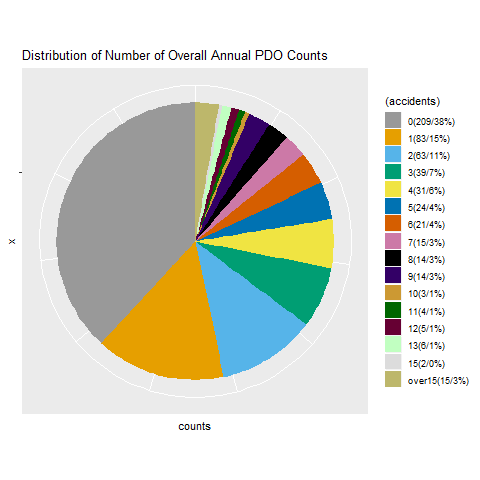
\includegraphics[width=3in]{image/p111.png}
\small
\end{minipage}
\begin{minipage}[t]{0.5\linewidth}
\centering
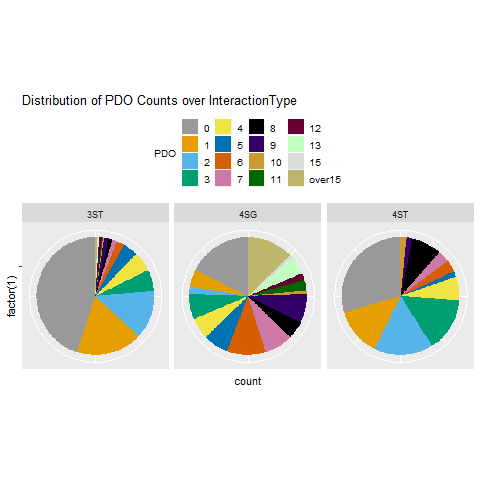
\includegraphics[width=3in]{image/p121_PDO.png}
\small
\end{minipage}
\caption{Pie chart of PDO}
\end{figure}

For the BC(possible injury or non-incapacitating injury) crashes, over one-half(59\%) of the intersections have 0 crash and 76\% of all intersections have less than 2 crashes. Like PDO, 4-way intersections tend to have larger number of BC crashes.

\begin{figure}[H]
\begin{minipage}[t]{0.5\linewidth}
\centering
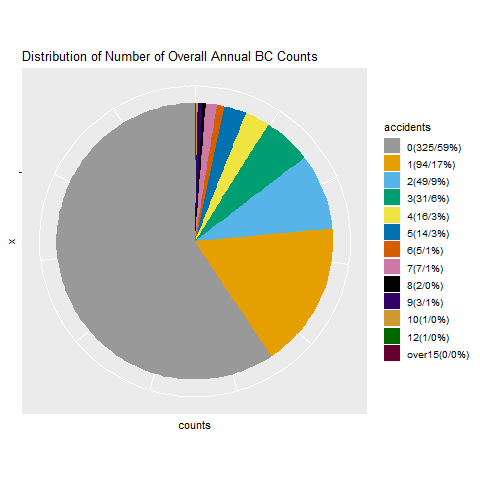
\includegraphics[width=3in]{image/p113.png}
\small
\end{minipage}
\begin{minipage}[t]{0.5\linewidth}
\centering
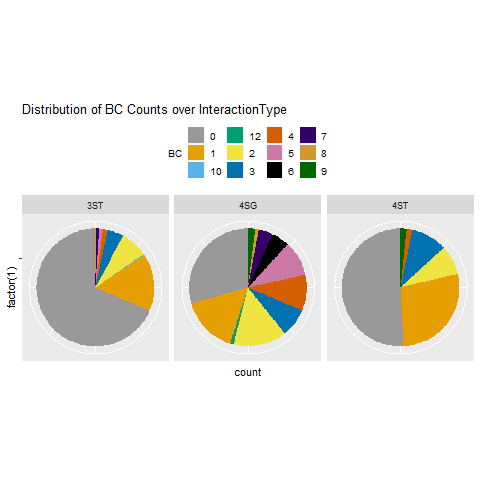
\includegraphics[width=3in]{image/p121_BC.png}
\small
\end{minipage}
\caption{Pie chart of BC}
\end{figure}

For the KA(fatal or incapacitating injury) crashes, only 0,1 and 2 crashes are observed. We can infer that Poisson or Negative Binomial distribution may not be suitable to fit the KA data. Quite similar to the conclusion above, 4SG and 4ST types have larger proportion of intersection with crashes.

\begin{figure}[H]
\begin{minipage}[t]{0.5\linewidth}
\centering
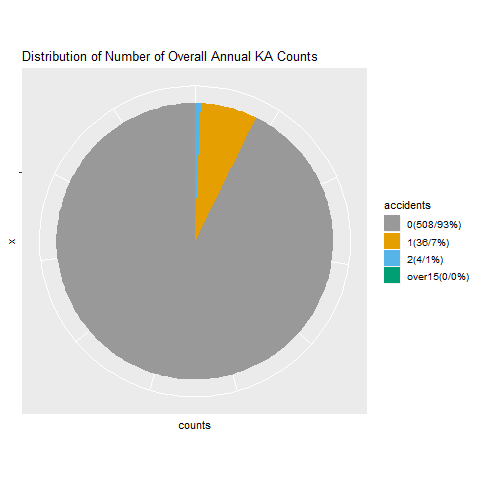
\includegraphics[width=3in]{image/p112.png}
\small
\end{minipage}
\begin{minipage}[t]{0.5\linewidth}
\centering
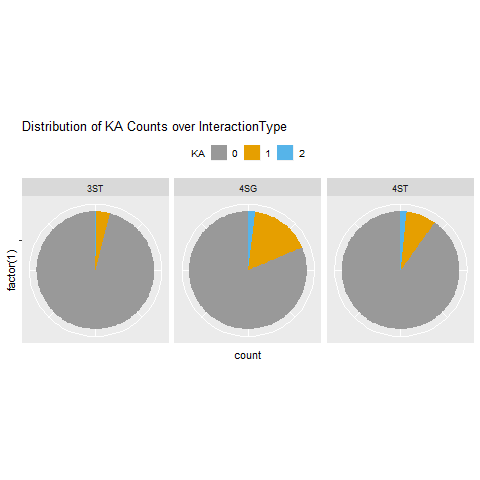
\includegraphics[width=3in]{image/p121_KA.png}
\small
\end{minipage}
\caption{Pie chart of KA}
\end{figure}

Comparing the overall distribution of 3 types of crashes, we can see that for all 3 types, 0 crash has the maximum proportion in all 548 intersection. PDO and BC have more possible count values with larger dispersions, which is a hint that it is not plausible to mix PDO, KA and BC observations together when we want to model the distribution of crashes. Also, variance exists between types of intersections. Since intersection type is a more fixed factor that is hard to change in real traffic, in the following parts, we will analyze the data controlling intersection type to get some plausible suggestions to reduce crashes based on other variables.

\subsection{Crash vs Qualitative Variables}

Next, we find some interesting relationship between crash and the 3 categorical variables, LIGHTING, APPROACH-LEFTTURN, and APPROACH-RIGHTTURNk.

\subsubsection{Lighting}

First, let's see the relationship between LIGHTING and crashes. There are 197 intersections without lighting in all 548(around 36\%) intersections. Overall, when not controlling intersection type, intersection without lighting tends to have fewer crashes than intersection with lighting in all 3 types of crashes. We can compare the proportion of 0 counts in the following bar chart of PDO. The bar chart of BC and KA has similar tendency which are contained in Appendix1.

When controlling intersection type, there are some interesting findings.

For PDO, in 3ST and 4SG types, partitioned data has same tendency with whole data while for 4ST group, there is lower proportion of observations with crash when there is lighting, which is opposite to the whole data. For BC and KA, partitioning with intersection type generates same result in each group as the whole set.

The plots infer that there might be a relationship between lighting and crash, but the effect is not very obvious from the plots. We will not take 4ST PDO group out for special consideration as these group has a quite small number of observations which may cause larger randomness.

\begin{figure}[H]
\begin{minipage}[t]{0.5\linewidth}
\centering
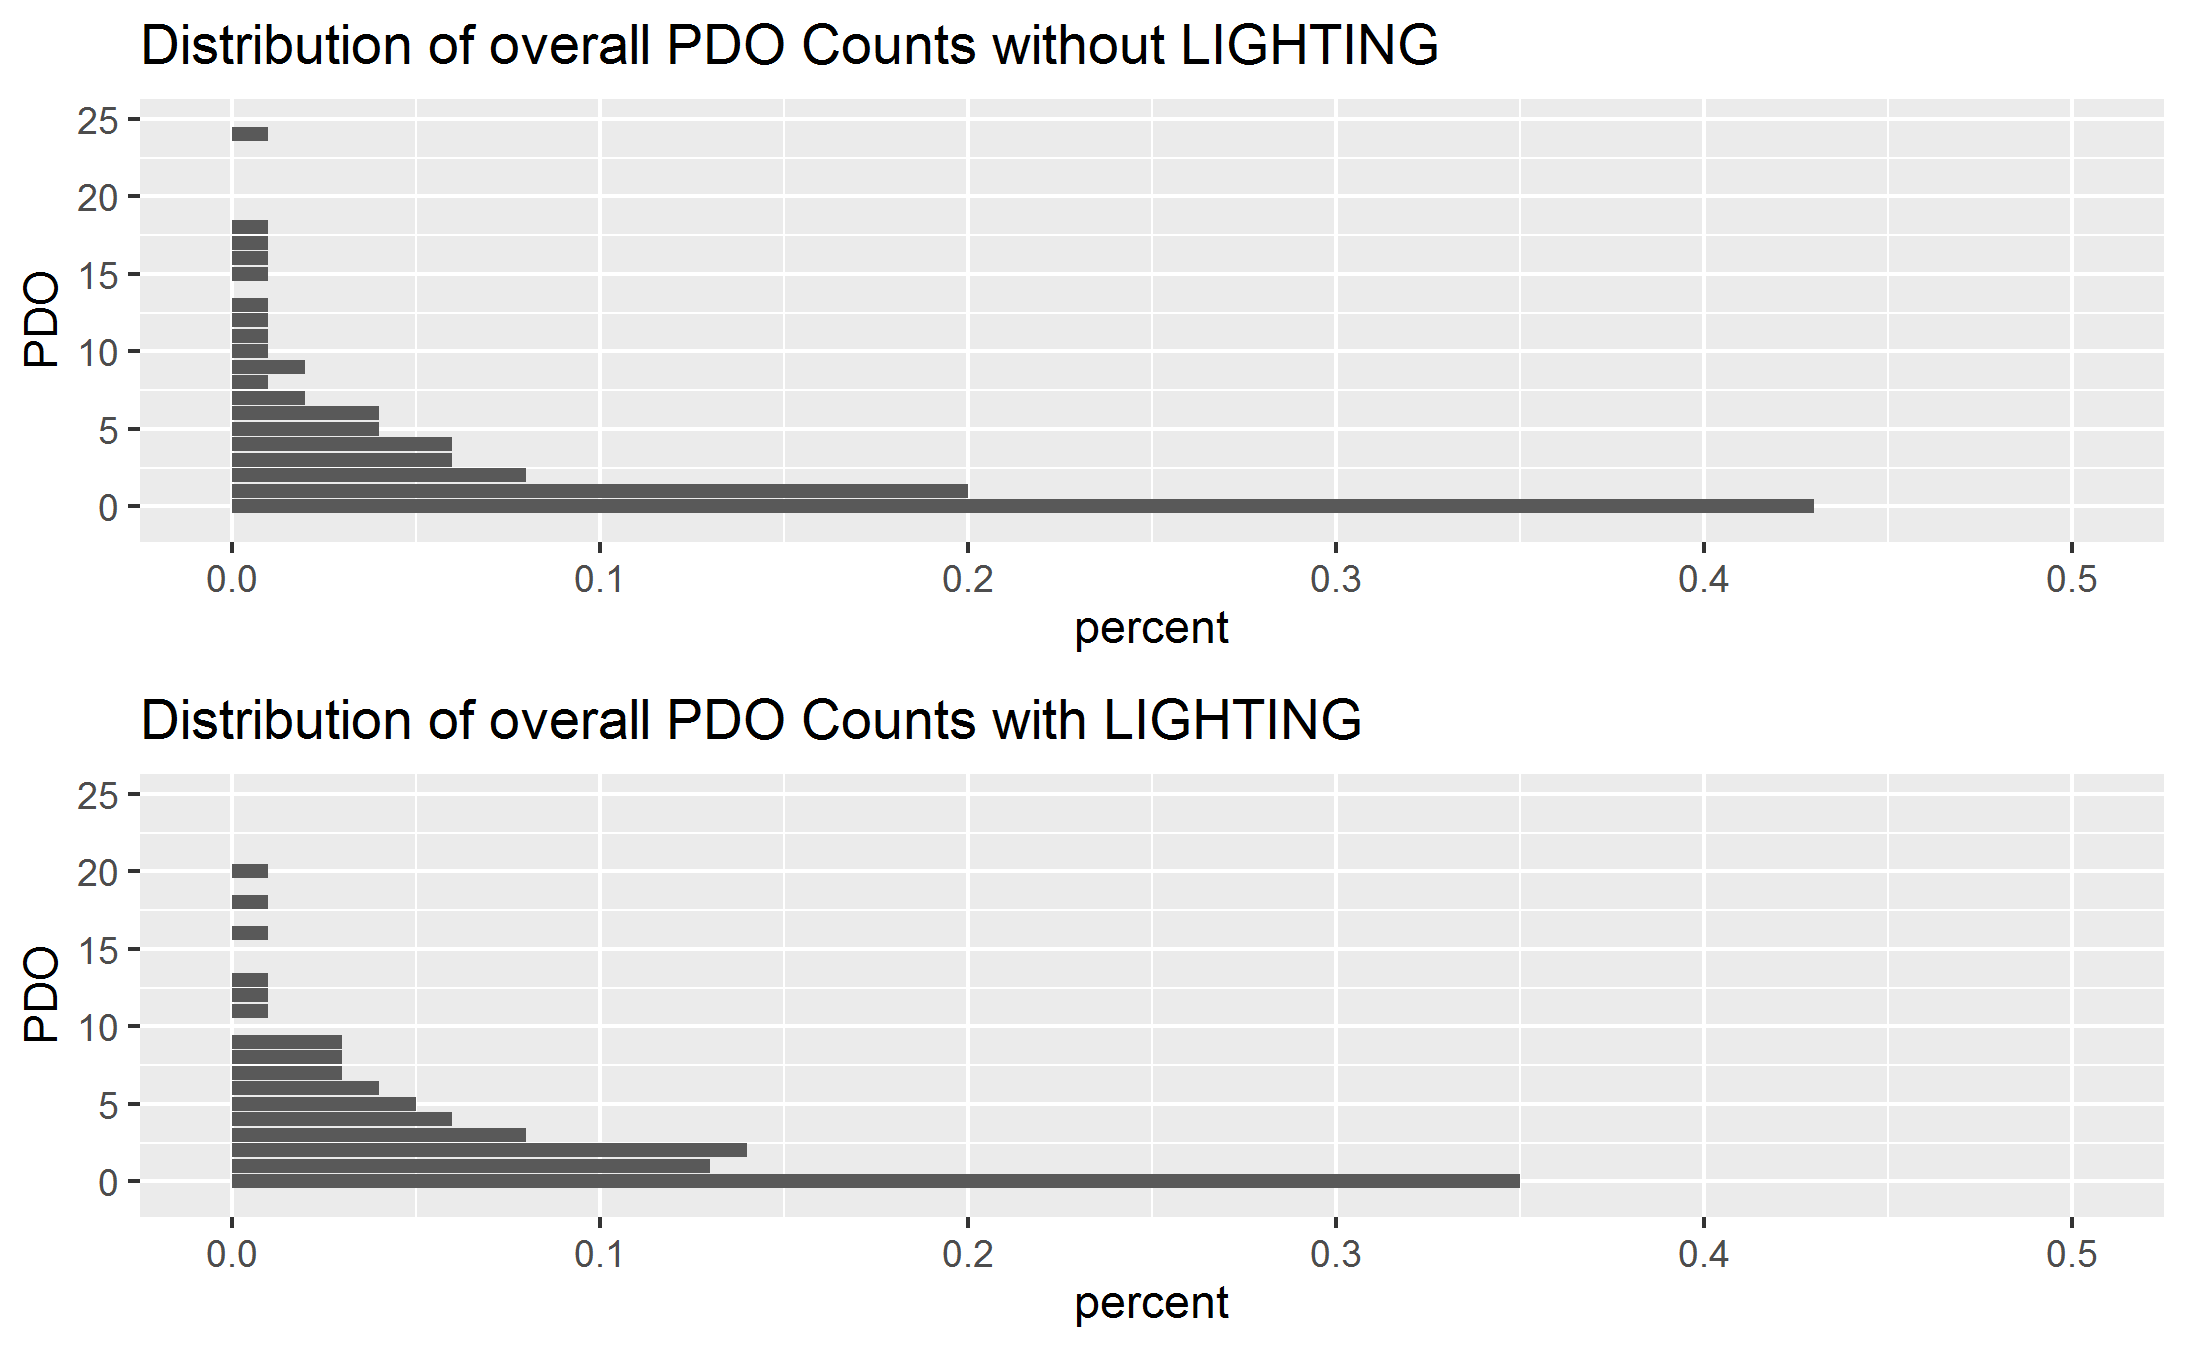
\includegraphics[width=3in]{image/LIGHTING_all_PDO.png}
\small
\end{minipage}
\begin{minipage}[t]{0.5\linewidth}
\centering
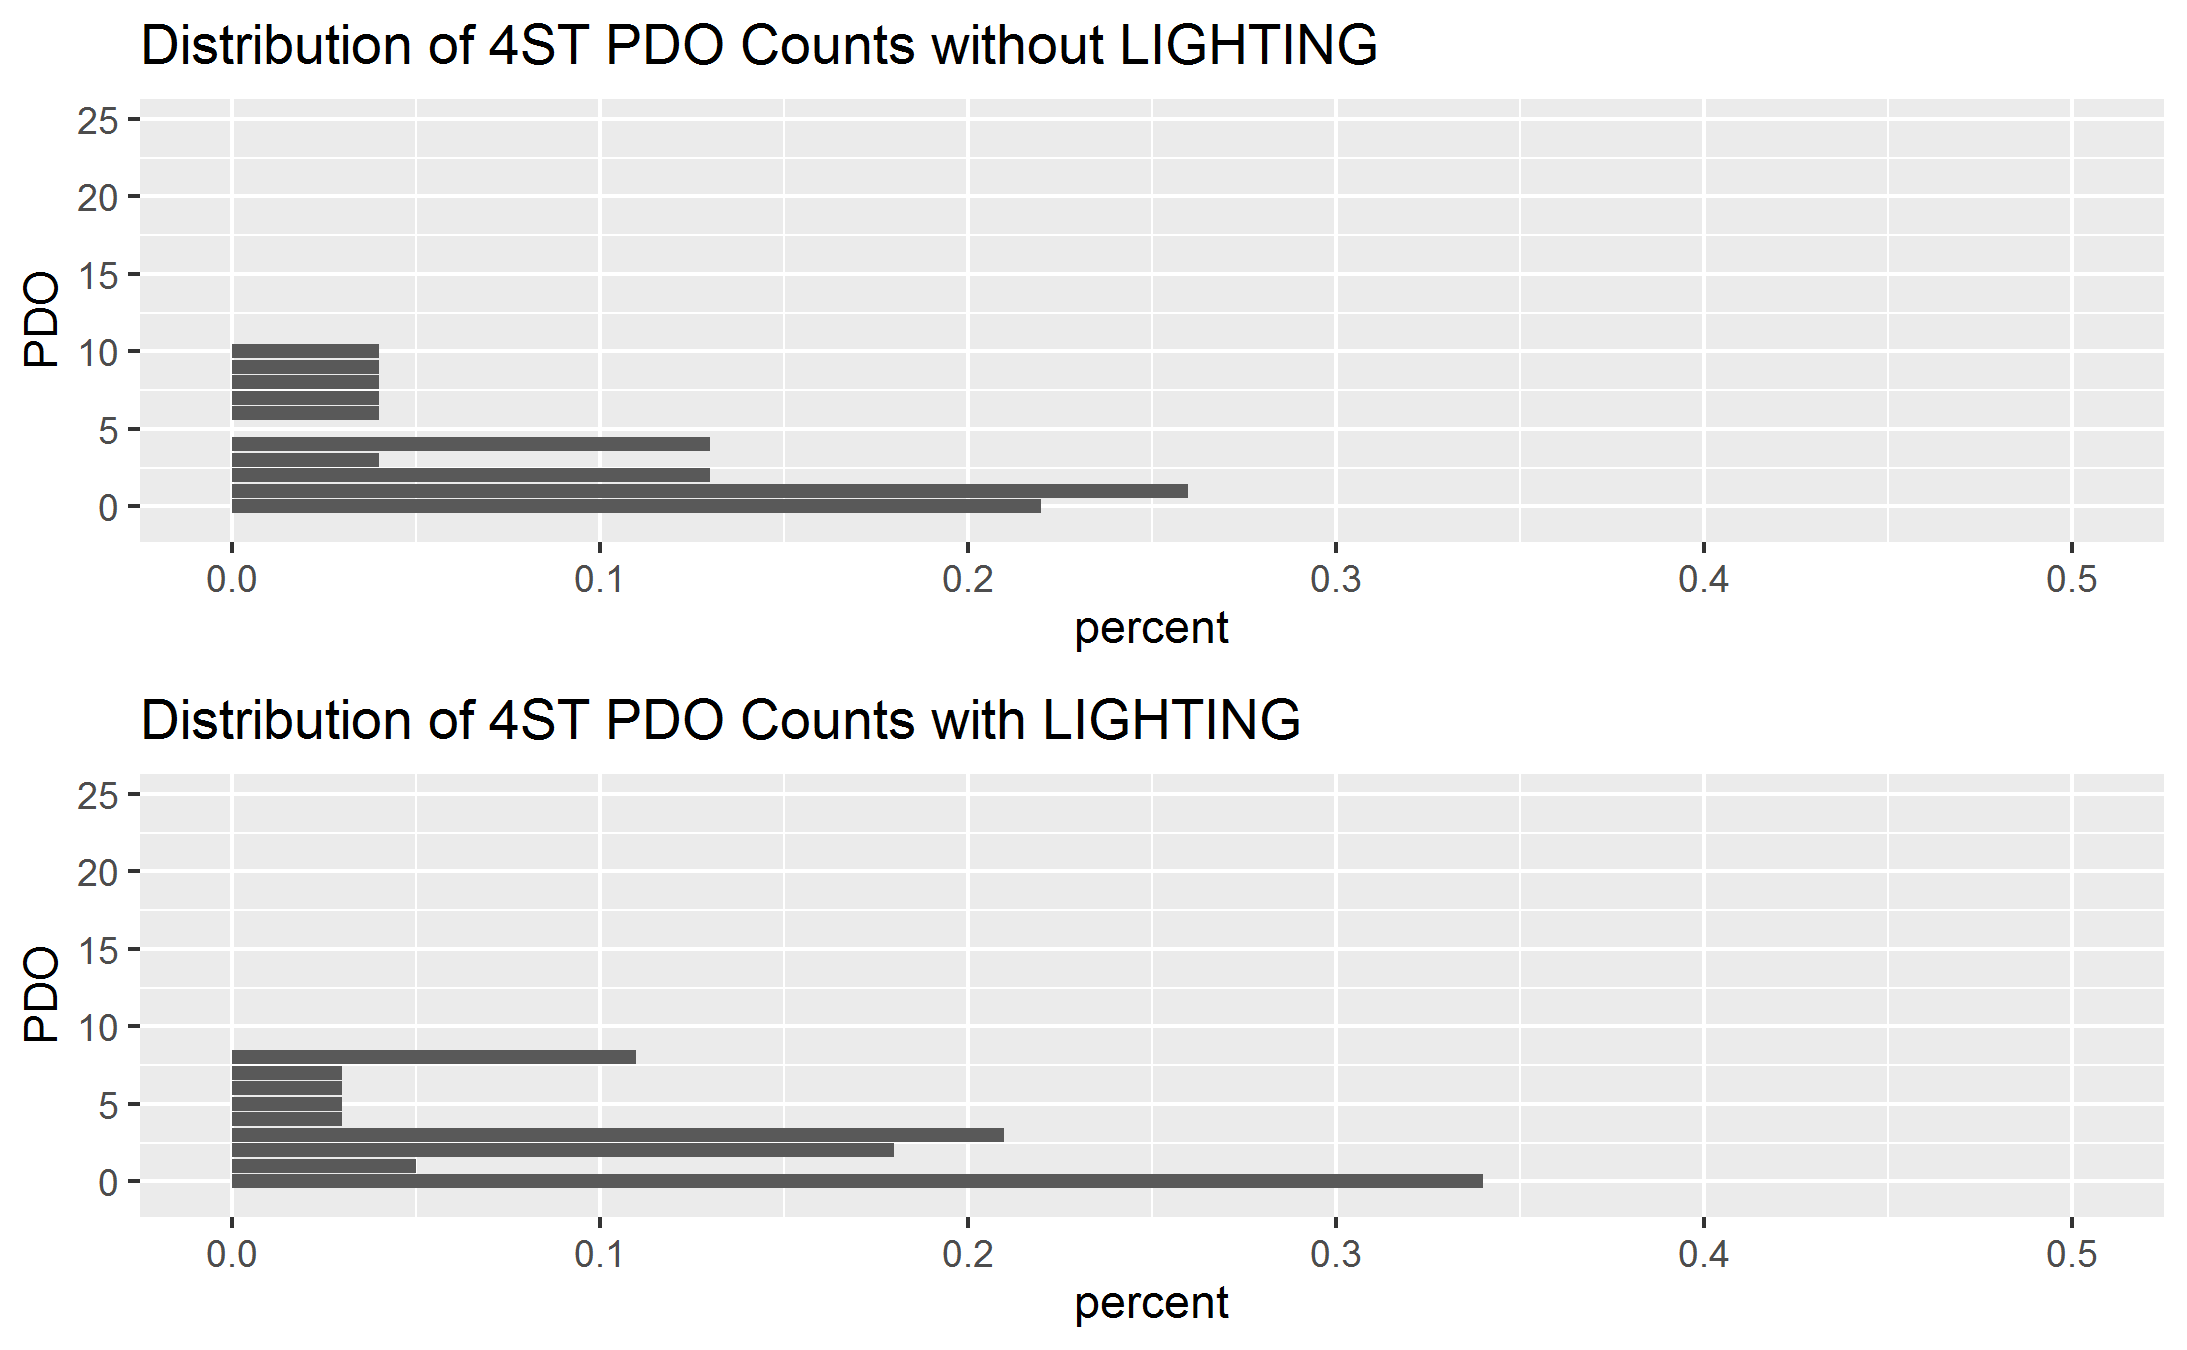
\includegraphics[width=3in]{image/LIGHTING_4ST_PDO.png}
\small
\end{minipage}
\caption{Bar Chart of Lighting}
\end{figure}

\subsubsection{Approach Left Turn and Approach Right Turn}

There are only 65 intersections with approach left-turn. When partitioning with intersection type, we get the following contingency table. From the table we can see that the counts get even smaller when separated into 3 type, there is not much sense to analyze with data further separated by crash type. There is similar problem with approach right-turn. Hence, we will not control crash type here and only care whether there is crash or not. So later discussion will be based on the generated binary columns "crash".

We observed similar association between these 2 variables and crash. Overall, when not controlling intersection type, intersection with approach left-turn or right turn lane has a higher crash rate, which infers that approach turn lane may has a positive relationship with car crashes. However, when we look into data grouped by intersection type, it is  shown that approach turn lane does not have big effect with 3ST and 4SG intersections, even shown slightly negative relationship. The effect is only obvious in 4ST groups, where the number of observations with left or right turn lane are quite small. Hence, the result of overall data and 4ST data may not be reliable.

Further, as same patterns are observed with right-turn and left-turn, we combine these 2 variables into a new binary variable, denoted as "TURN", where "1" stands for there exists an approaching turn and "0" else. The follow graph is made with combined column. (Separated result is in Appendix.)

\begin{table}[H]
\caption{Intersection vs Turns}
\centering
\begin{tabular}{|c|c|c|c|}
\hline
Observations      & 3ST & 4ST & 4SG \\
\hline
Without Left-turn & 368 & 58  & 57  \\
\hline
With Left-turn    & 17  & 44  & 4   \\
\hline
\end{tabular}
\end{table}


\begin{figure}[H]
\begin{minipage}[t]{0.5\linewidth}
\centering
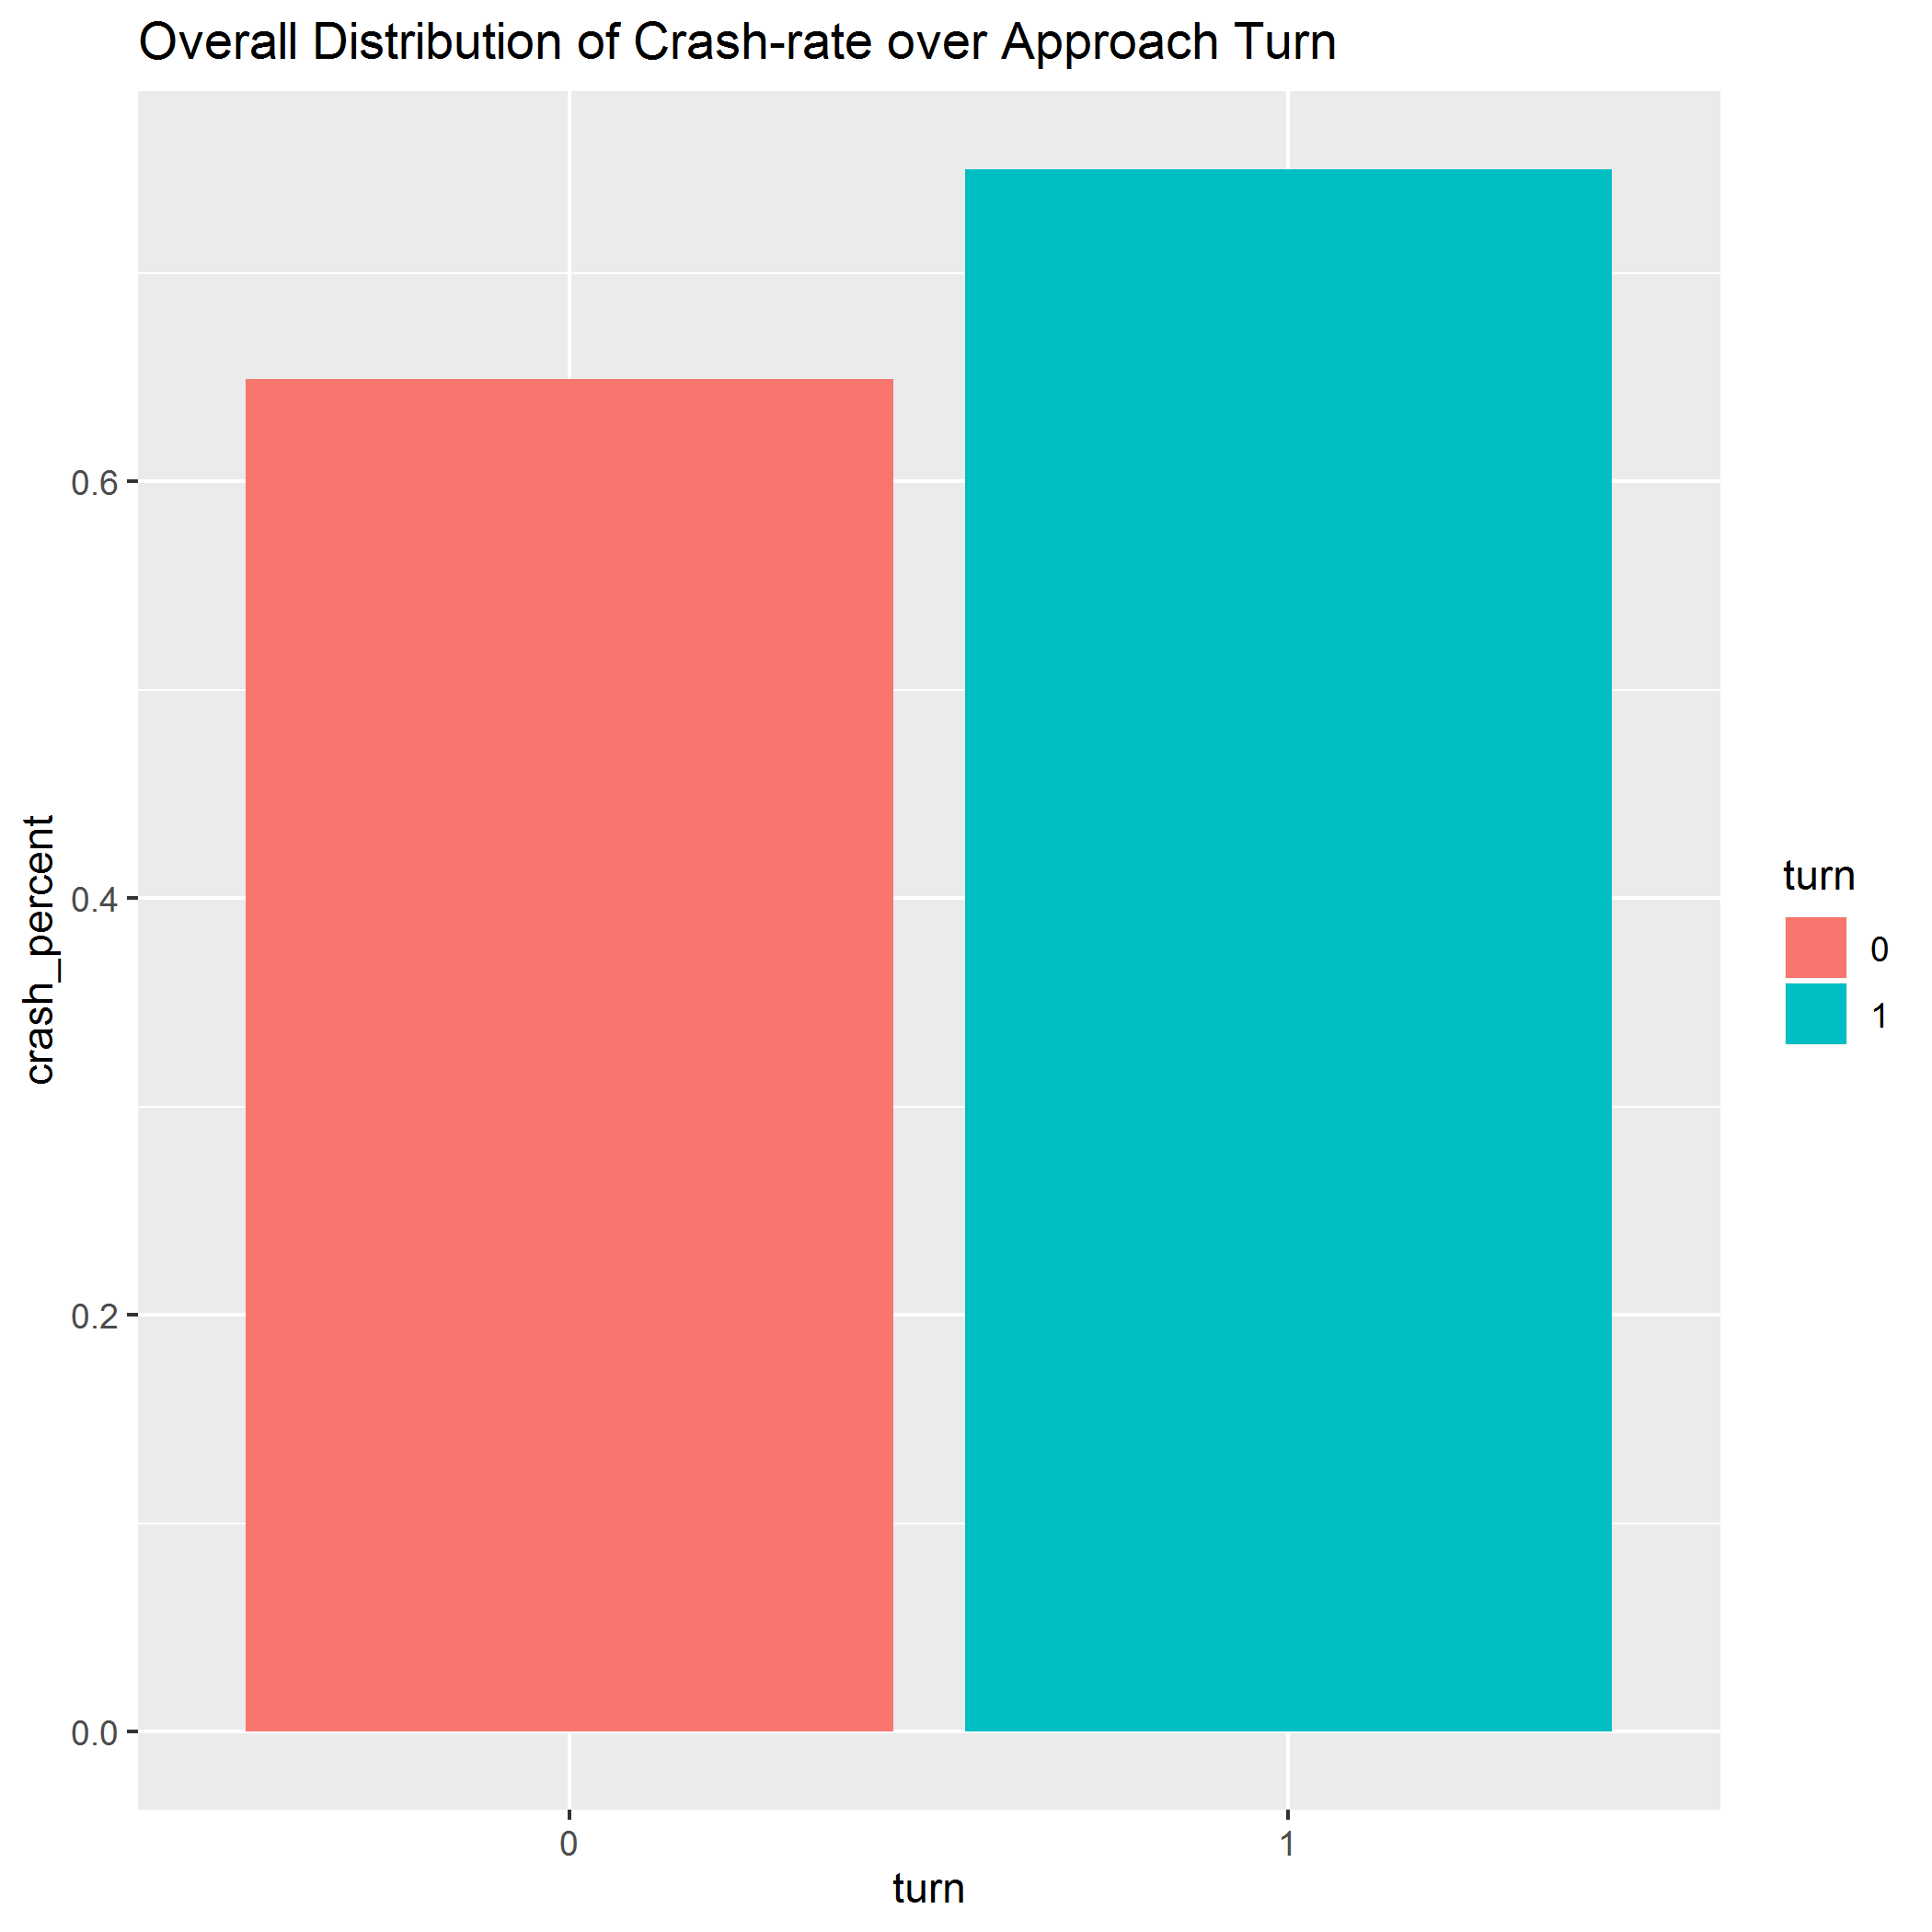
\includegraphics[width=3in]{image/approach-turn-all.png}
\small
\end{minipage}
\begin{minipage}[t]{0.5\linewidth}
\centering
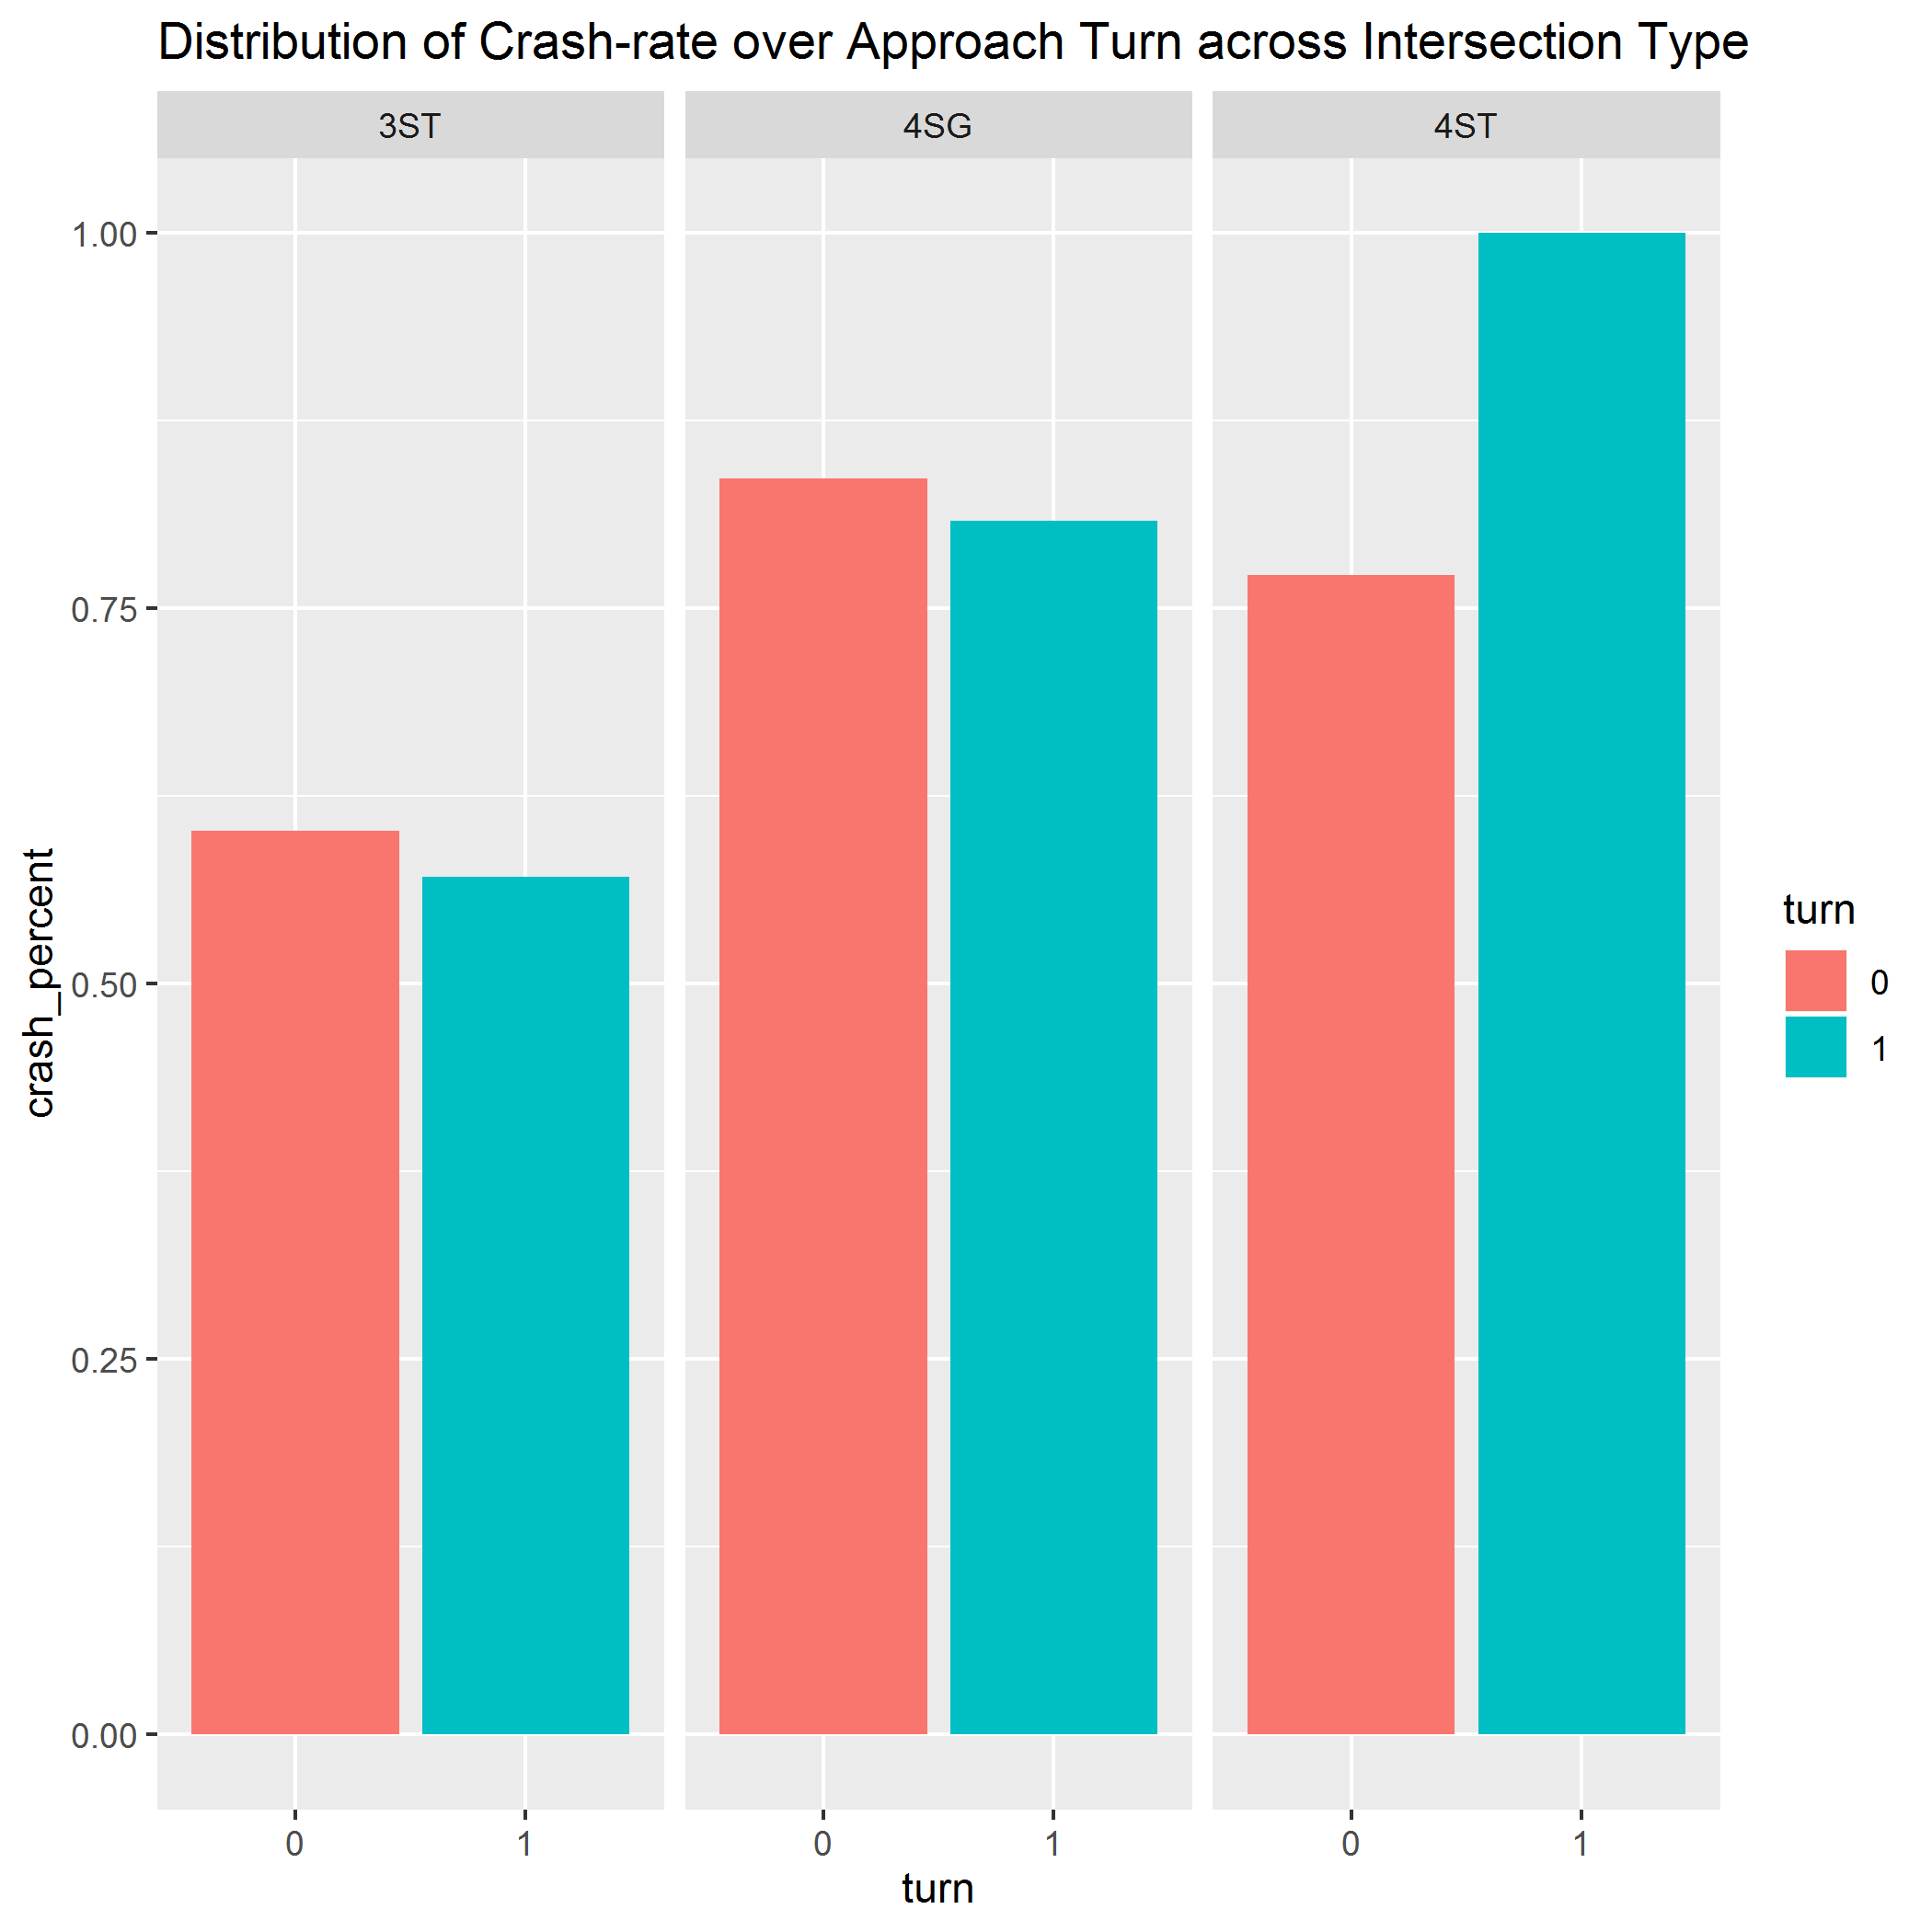
\includegraphics[width=3in]{image/approach-turn.png}
\small
\end{minipage}
\caption{Bar Chart of Approach Left Turn}
\end{figure}

\subsection{Crash vs Quantitative Variables}

Also, there is likely to exist some association between AADT-MAJOR, AADT-MINOR, SKEW-ANGLE and crash.

\subsubsection{AADT-MAJOR and AADT-MINOR}

Selected graphs are shown in this part.

We mainly apply the notched box-plot here to compare the distribution of AADT in intersection of crashes with intersection with no crash. The discussion is separated for each crash type. The first 3 box plots below show significant difference on median of overall distribution as the notches do not overlap. This infers that generally, the intersections with crash has higher level of AADT-Major in all 3 types of crashes.

After controlling the intersection type, all partitioned data shows same pattern that higher AADT-Major appears in group with crash. However, for PDO and BC, the difference is only significant in 3ST group and for KA, no difference is significant.

\begin{figure}[H]
\begin{minipage}[t]{0.5\linewidth}
\centering
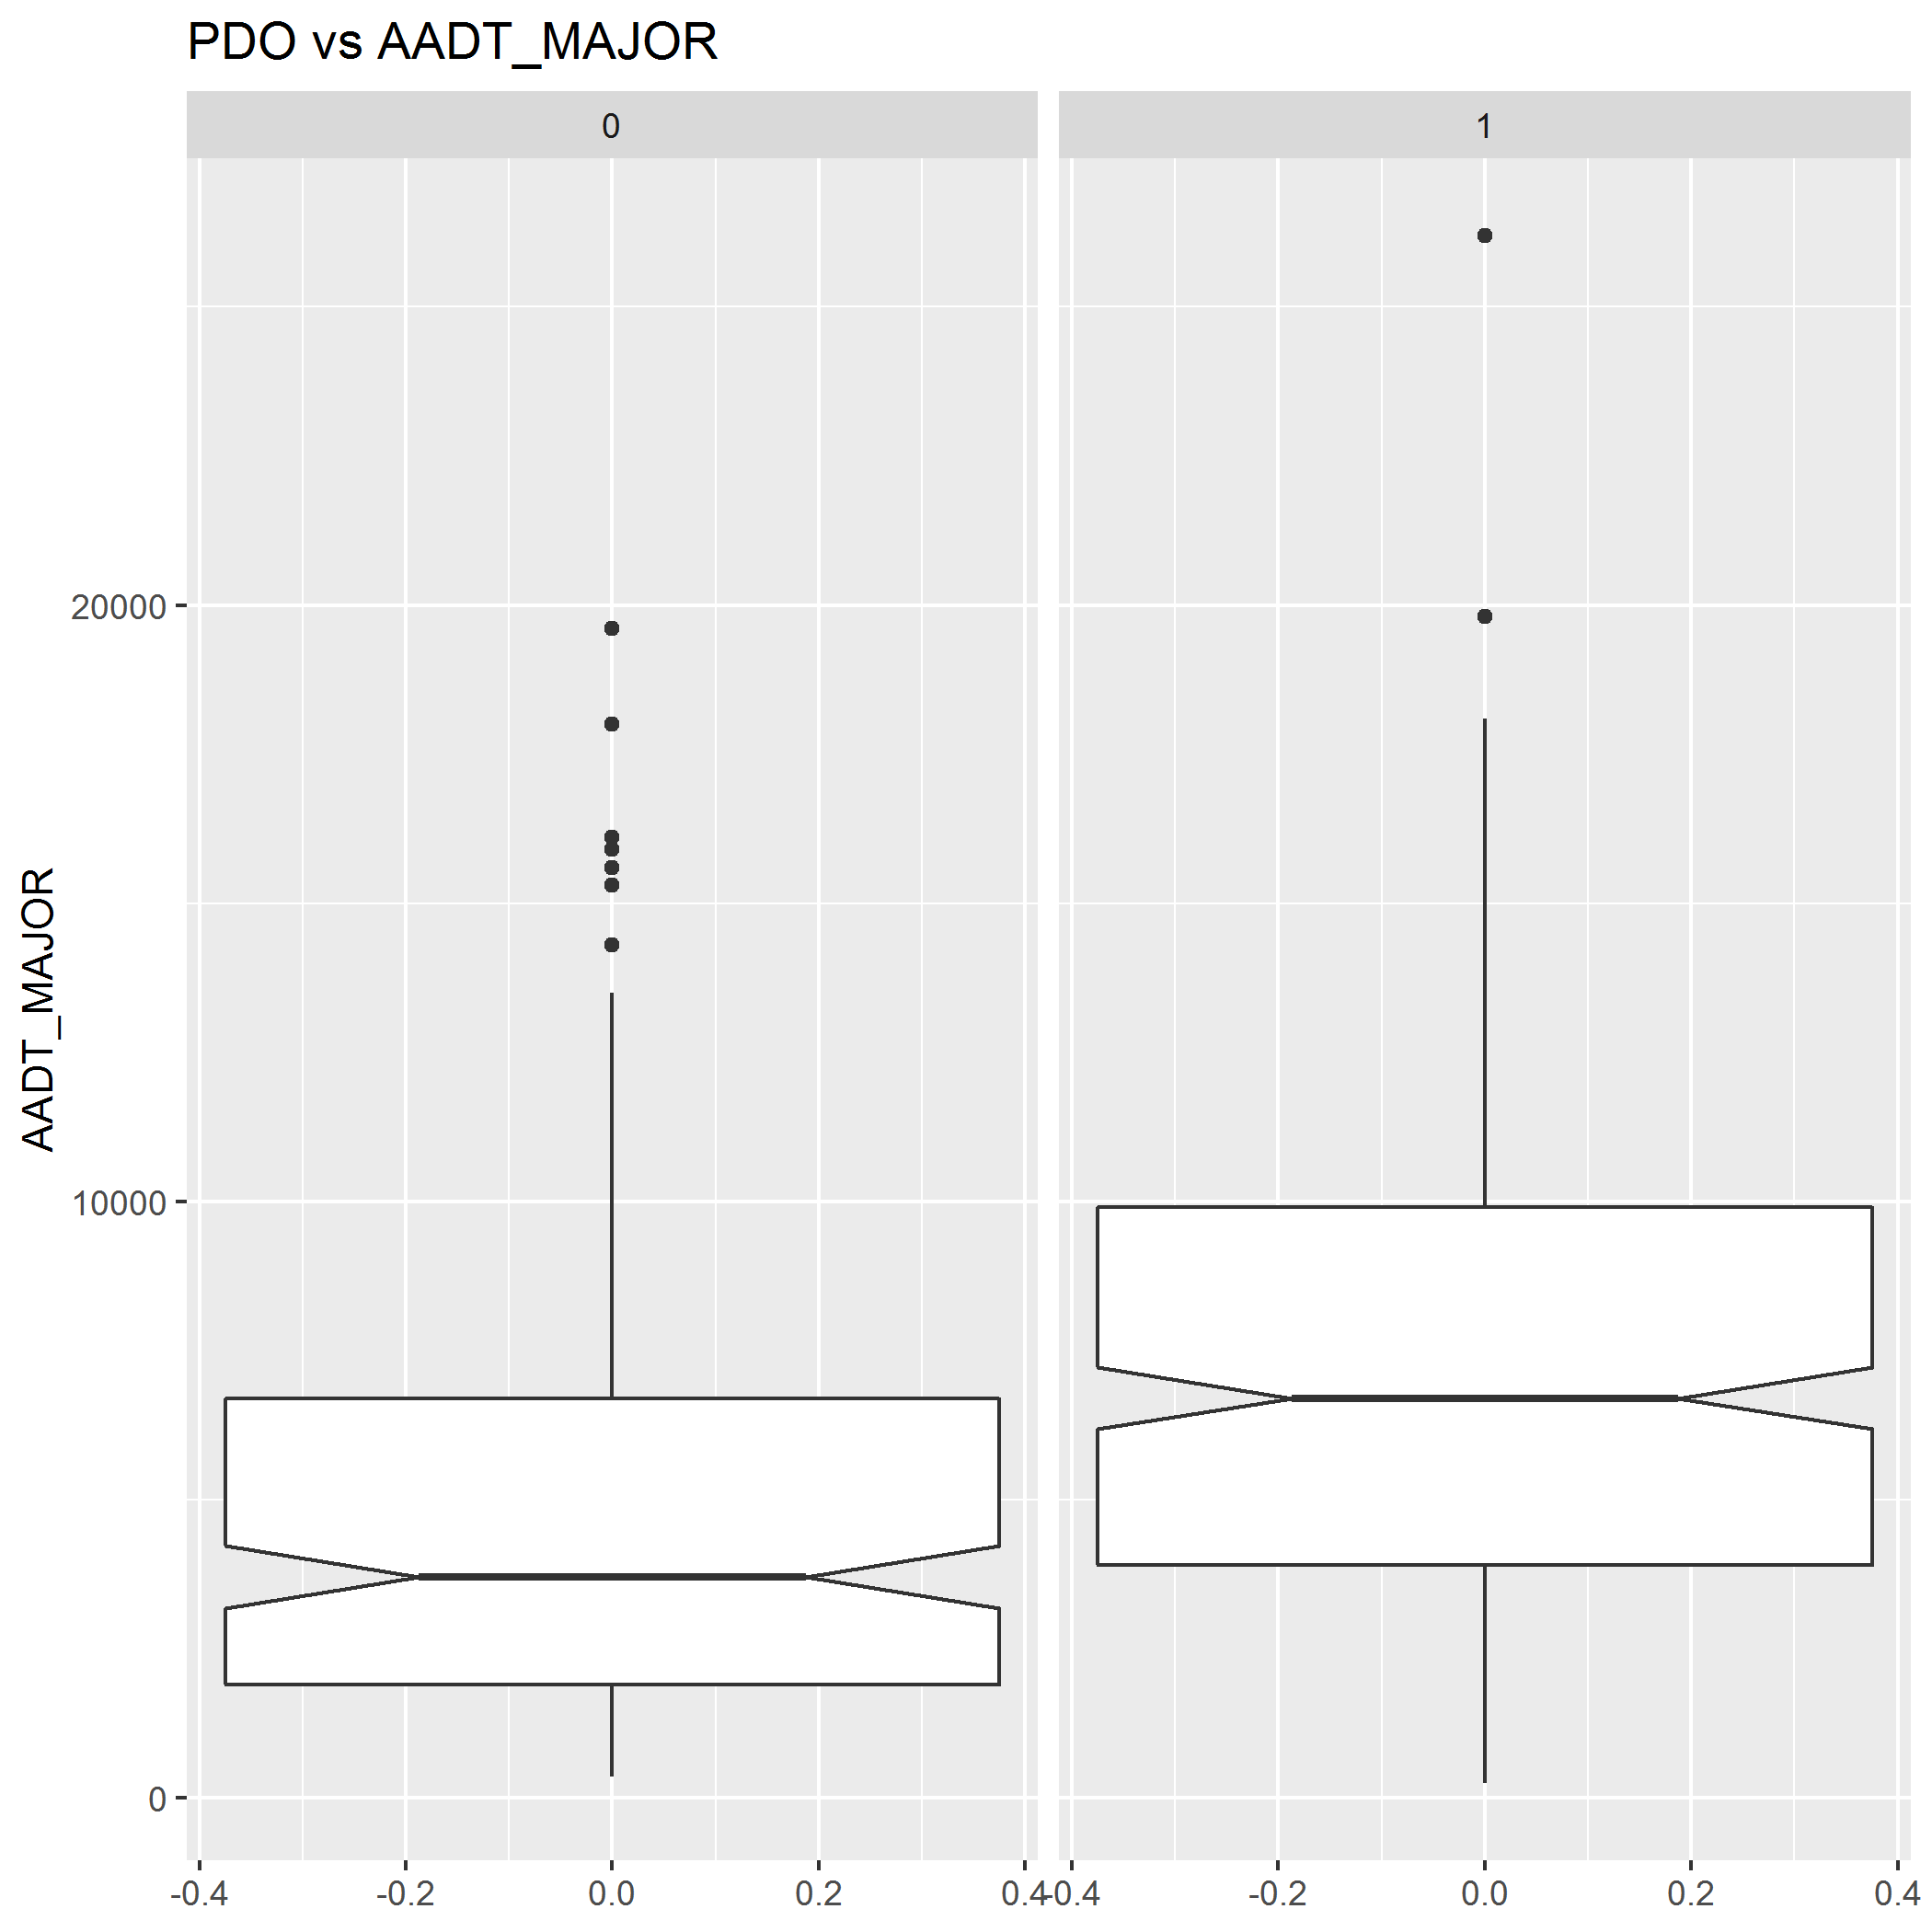
\includegraphics[width=3in]{image/major_all_pdo.png}
\small
\end{minipage}
\begin{minipage}[t]{0.5\linewidth}
\centering
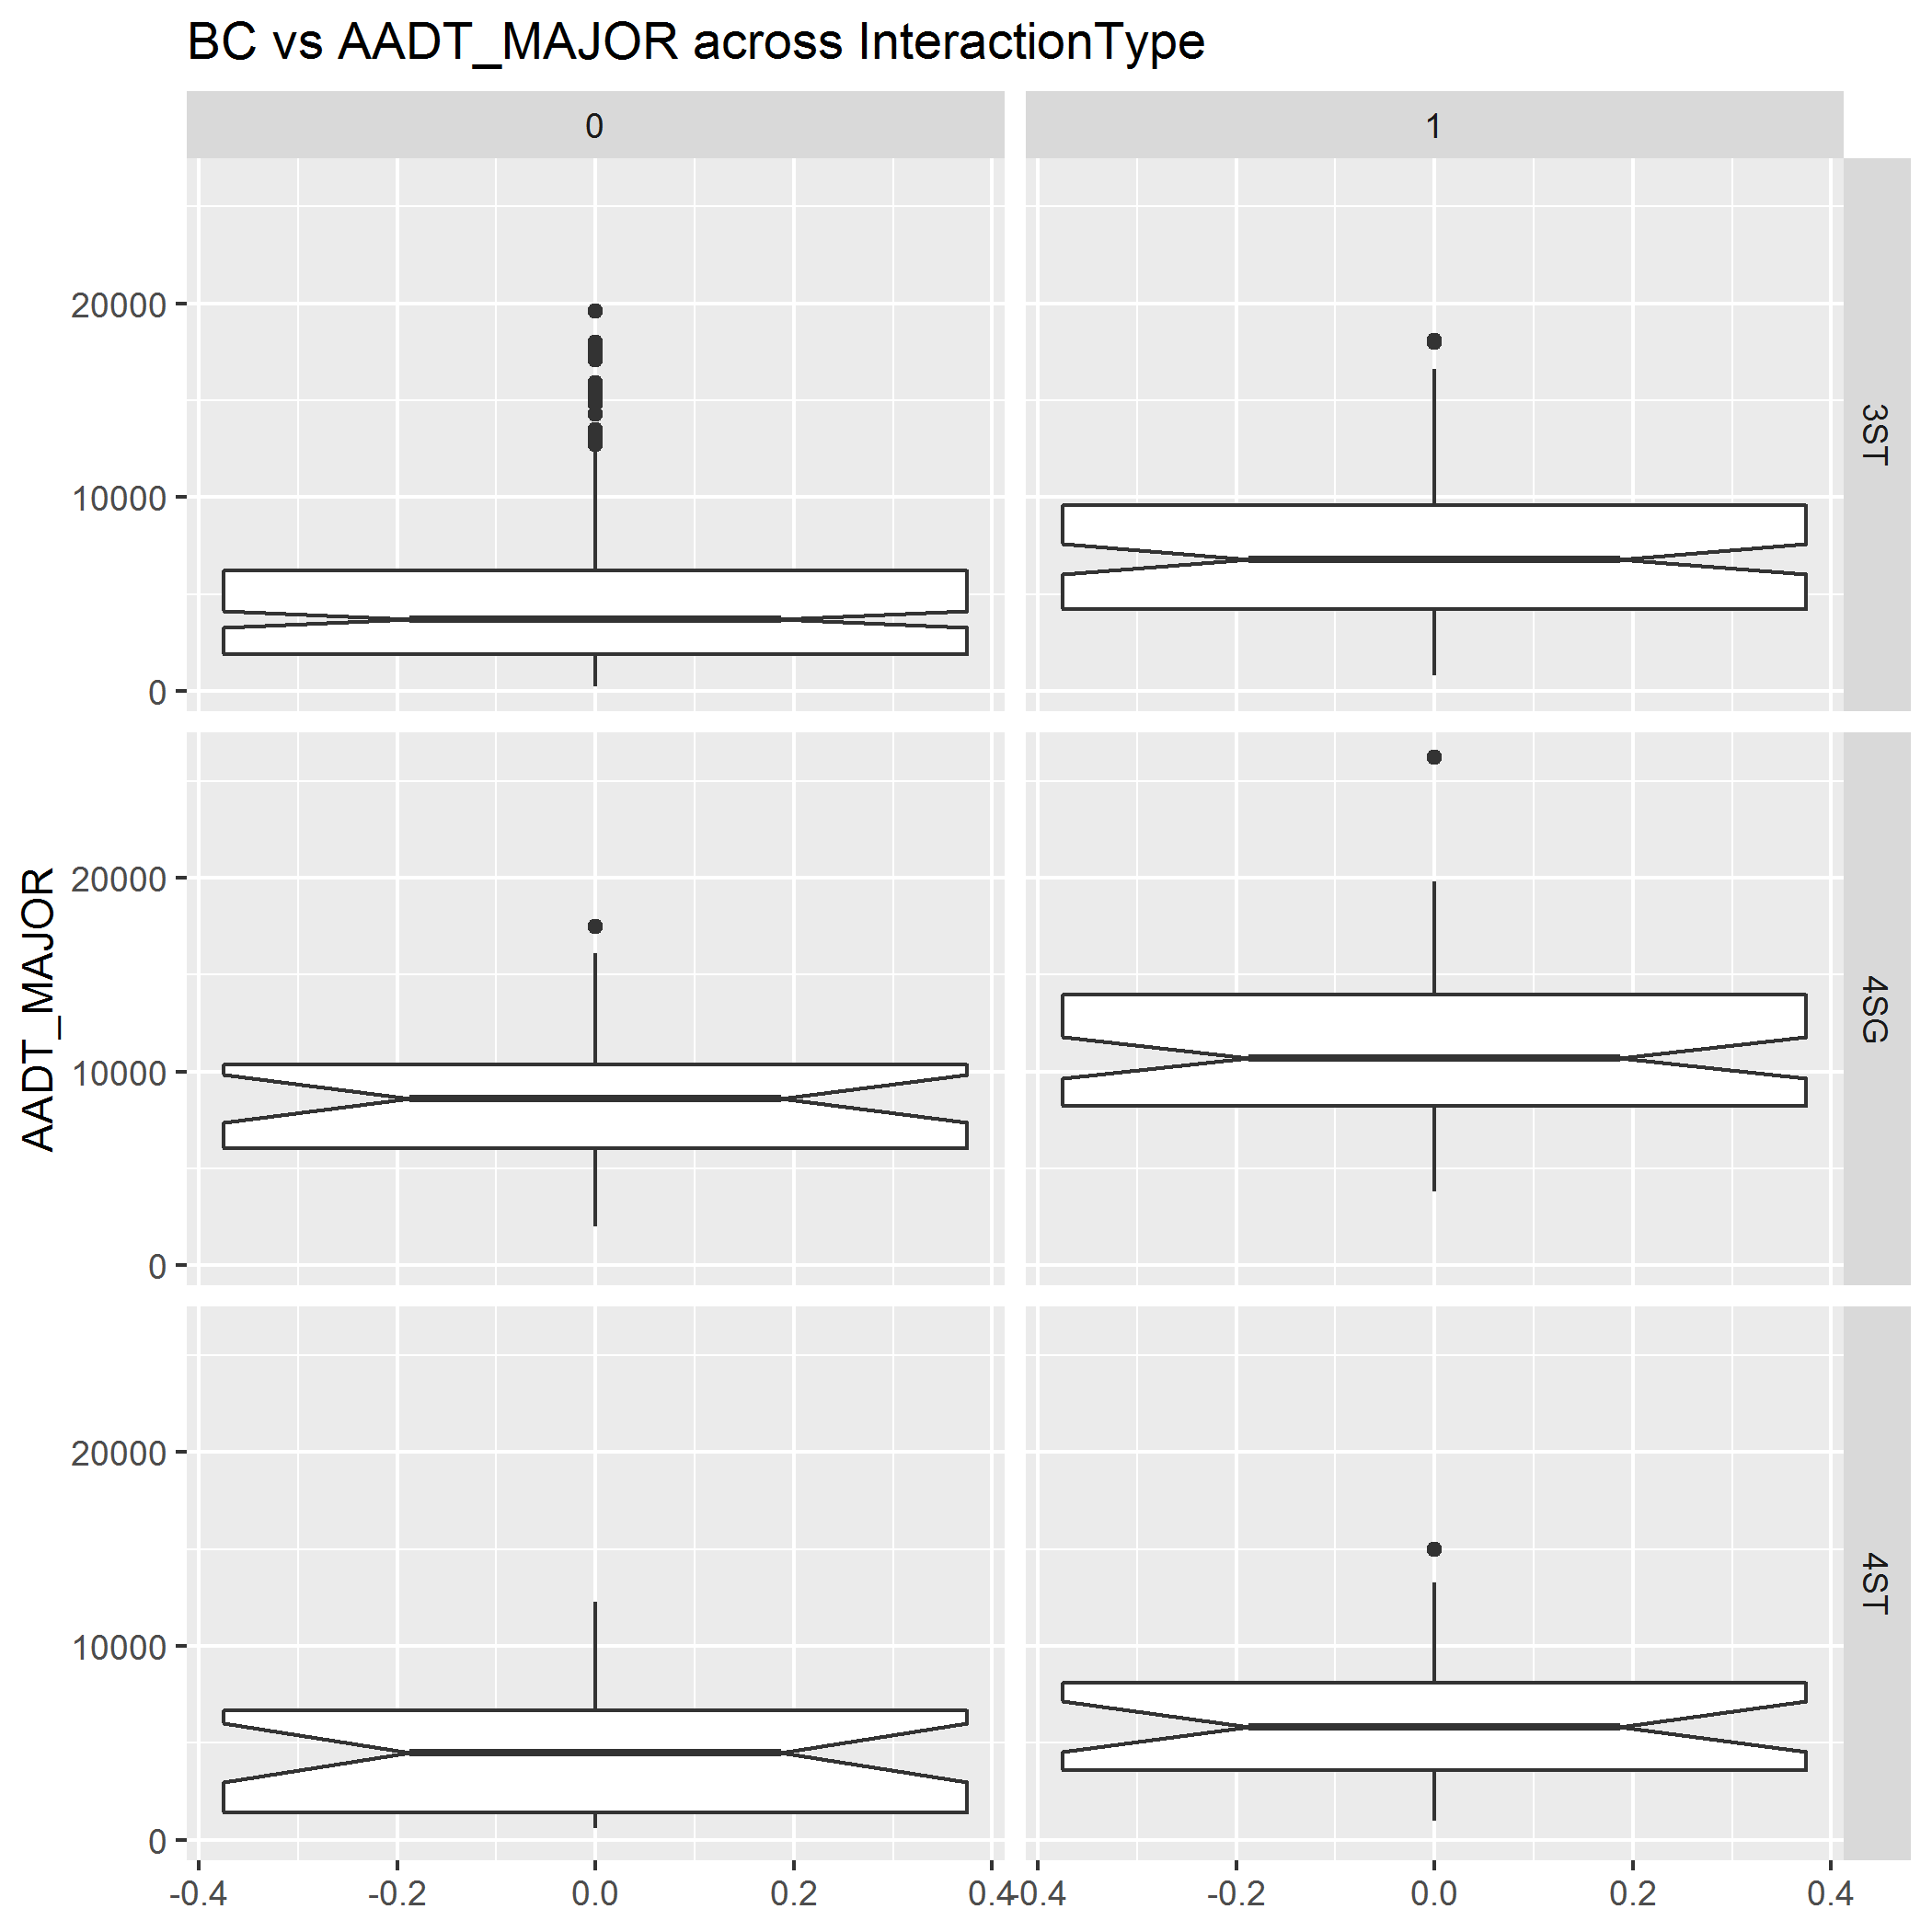
\includegraphics[width=3in]{image/major_bc.png}
\small
\end{minipage}
\caption{Boxplot of AADT-Major}
\end{figure}

For AADT-Minor, AADT-Minor is significantly larger in intersection with crash when exploring overall data for all of PDO, KA and BC. When taking intersection type into consideration, for 3ST group, same patterns are observed as overall data that the difference are all significant. However, opposite pattern occurs in 4SG group that intersection with crash has a lower AADT-MINOR value. The opposite difference of sample median between the with-crash and without-crash group is significant in PDO crash. For 4ST group, all difference in median is not significant.

\begin{figure}[H]
\begin{minipage}[t]{0.5\linewidth}
\centering
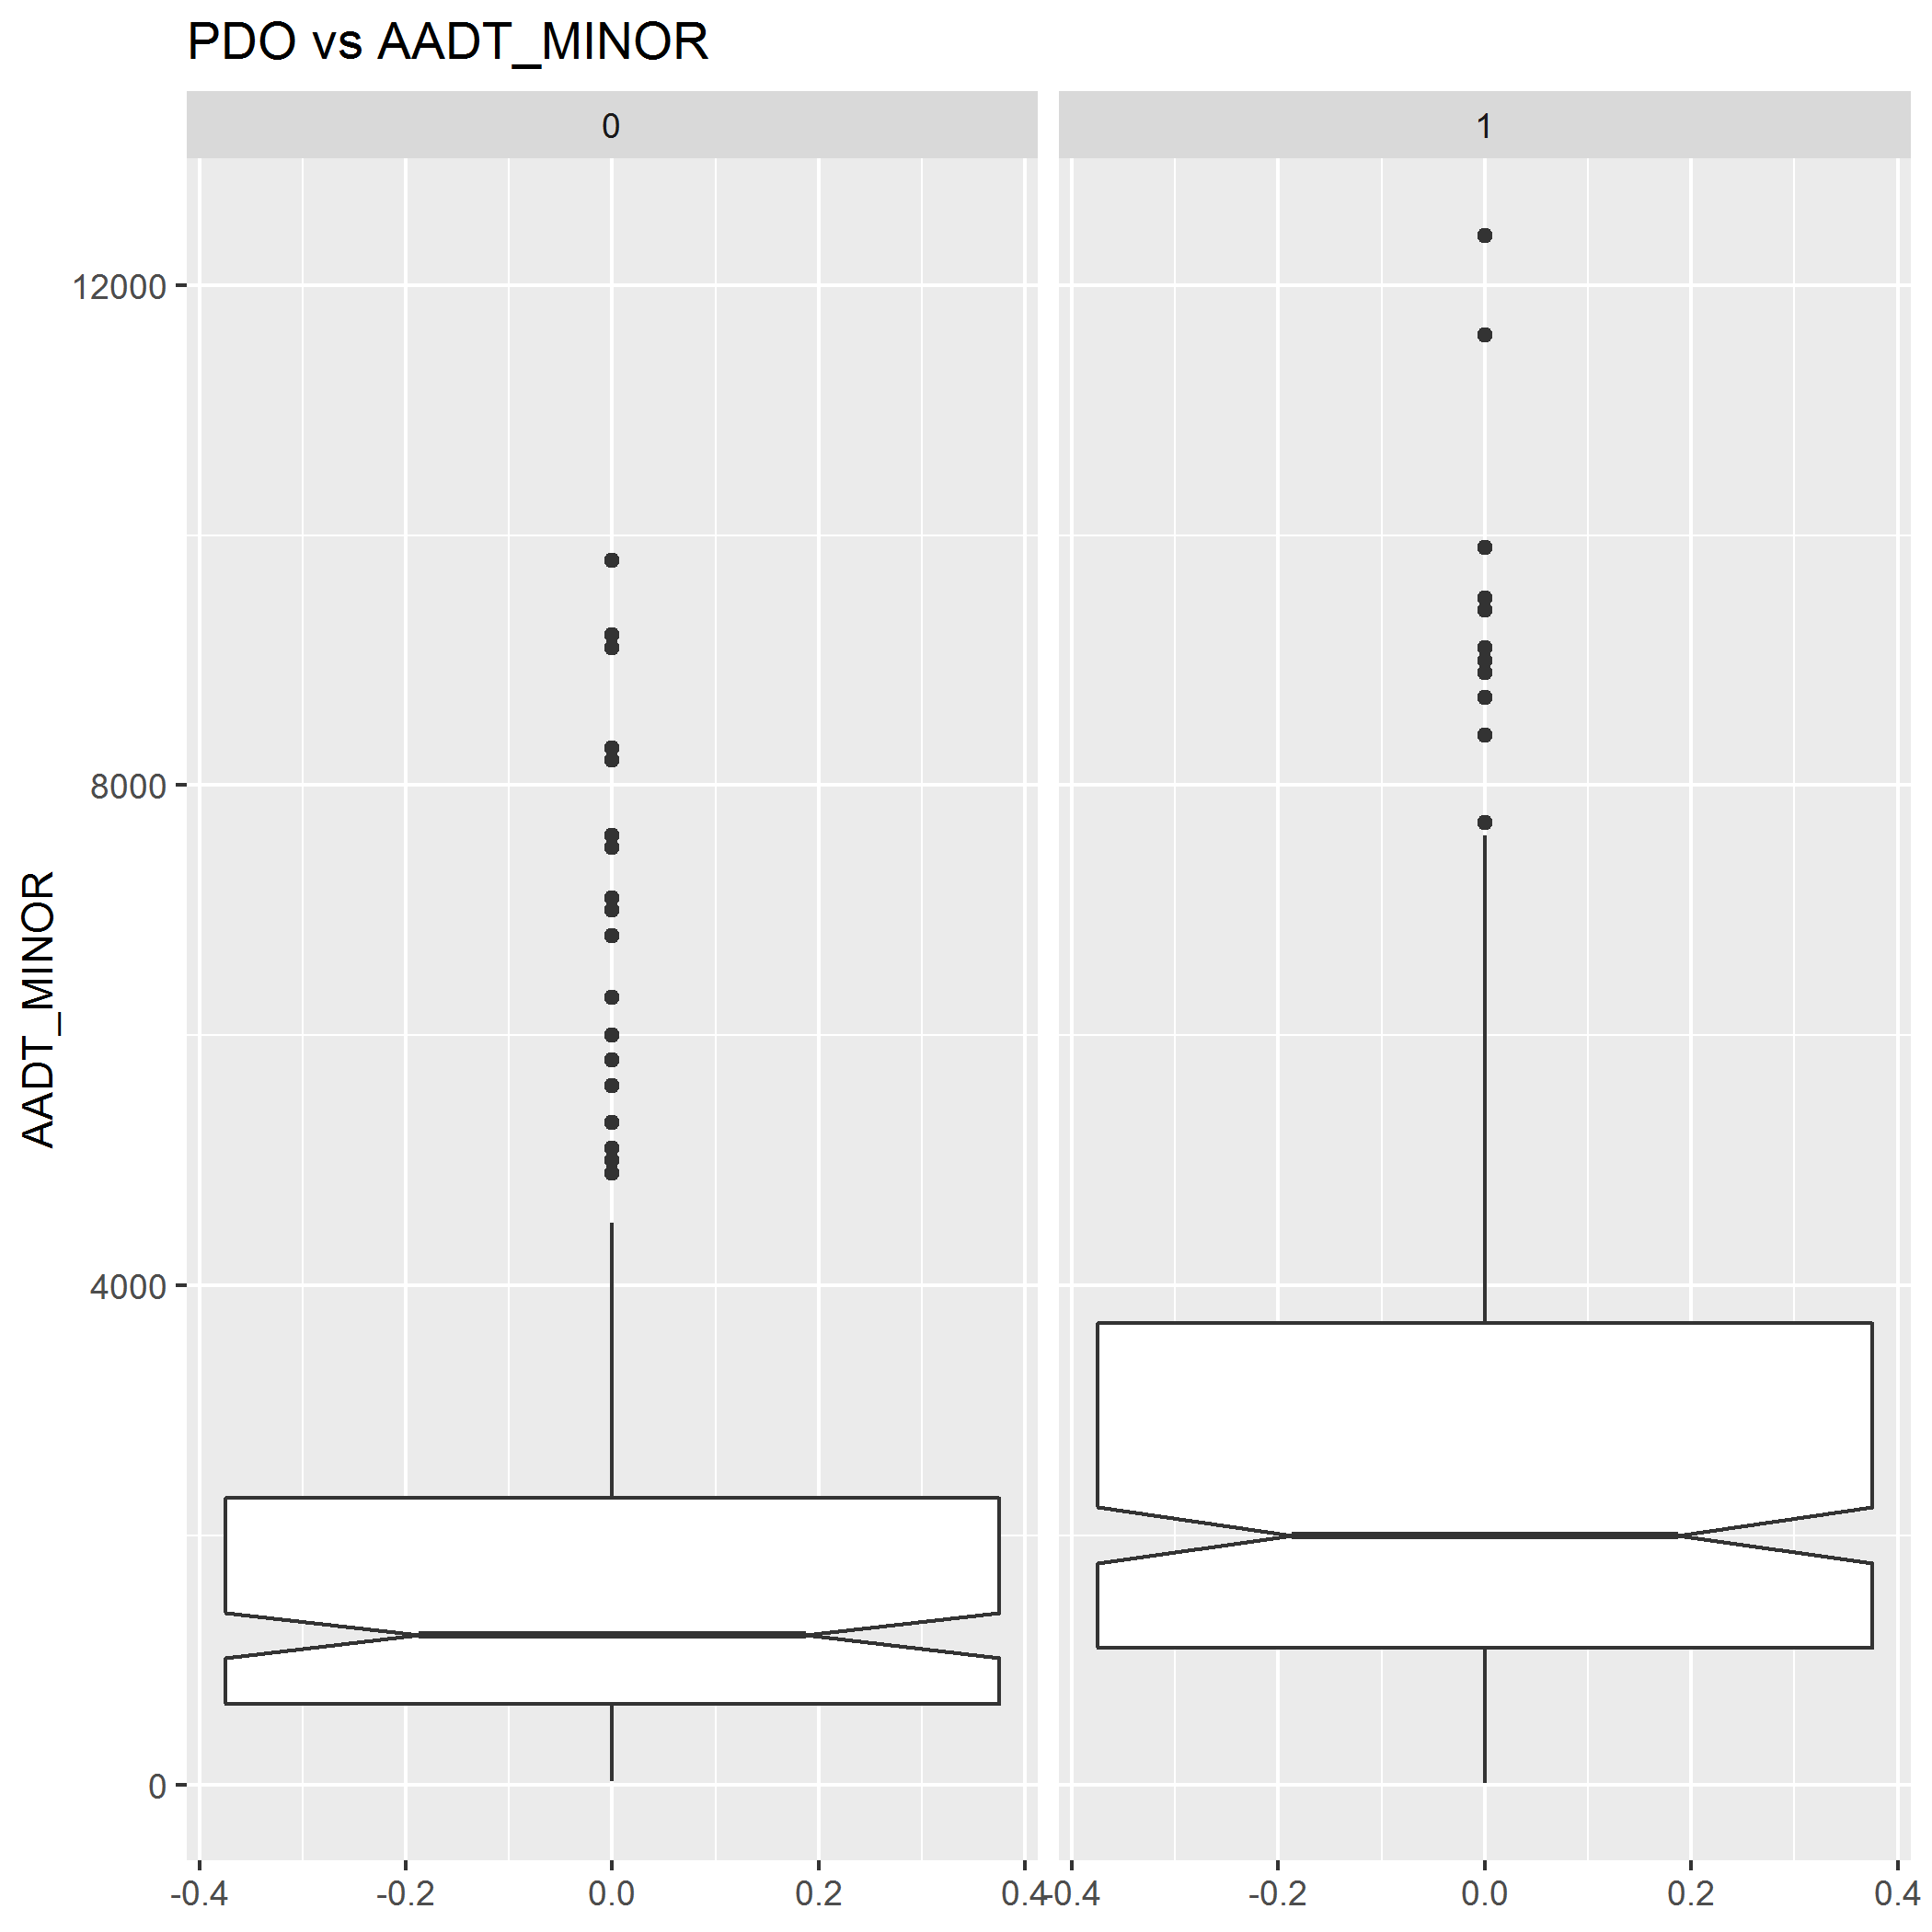
\includegraphics[width=3in]{image/minor_all_pdo.png}
\small
\end{minipage}
\begin{minipage}[t]{0.5\linewidth}
\centering
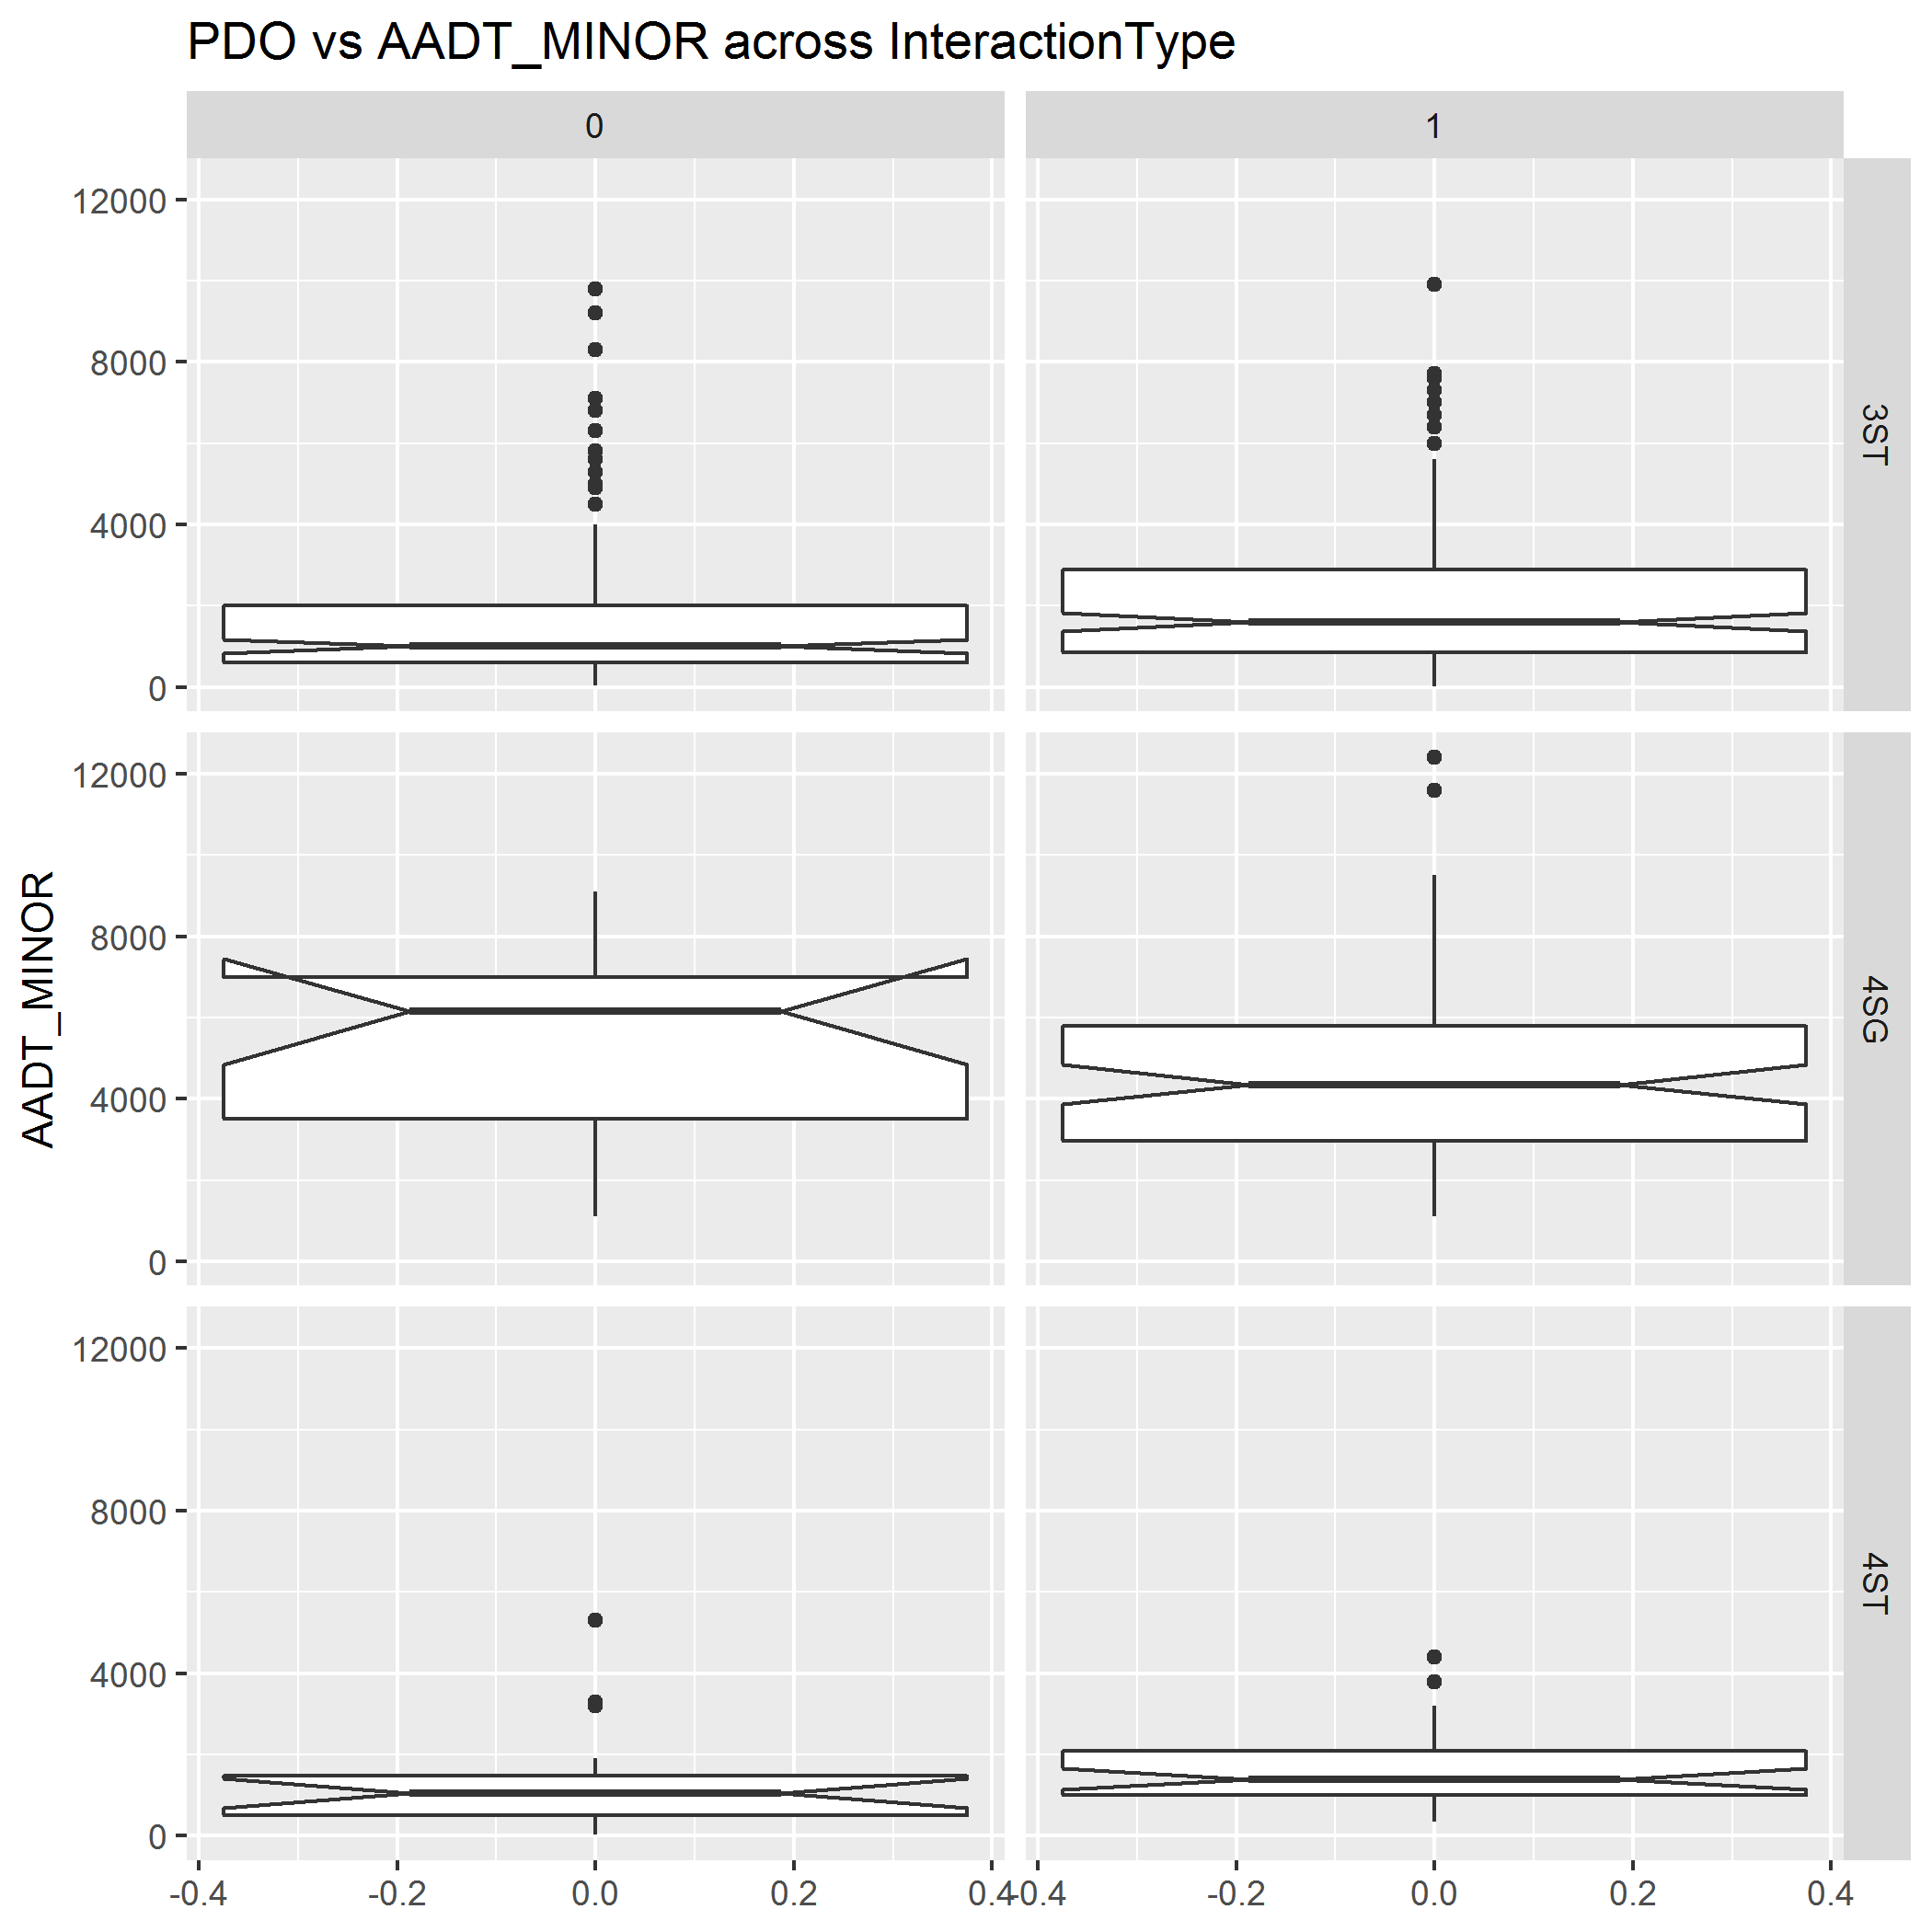
\includegraphics[width=3in]{image/minor_pdo.png}
\small
\end{minipage}
\caption{Boxplot of AADT-Minor}
\end{figure}

\subsubsection{Skew Angle}

For Skew Angle, we apply notched box plot also. In all 3 types of crash, groups with crash have smaller median for skew angle while the difference is only significant in KA crash type. When controlling intersection type, only the 3ST intersection and PDO crash group shows significant larger skew angle median in no crash group. All other are insignificant. 4SG group get insignificant opposite pattern in PDO and BC crash.

\begin{figure}[H]
\begin{minipage}[t]{0.5\linewidth}
\centering
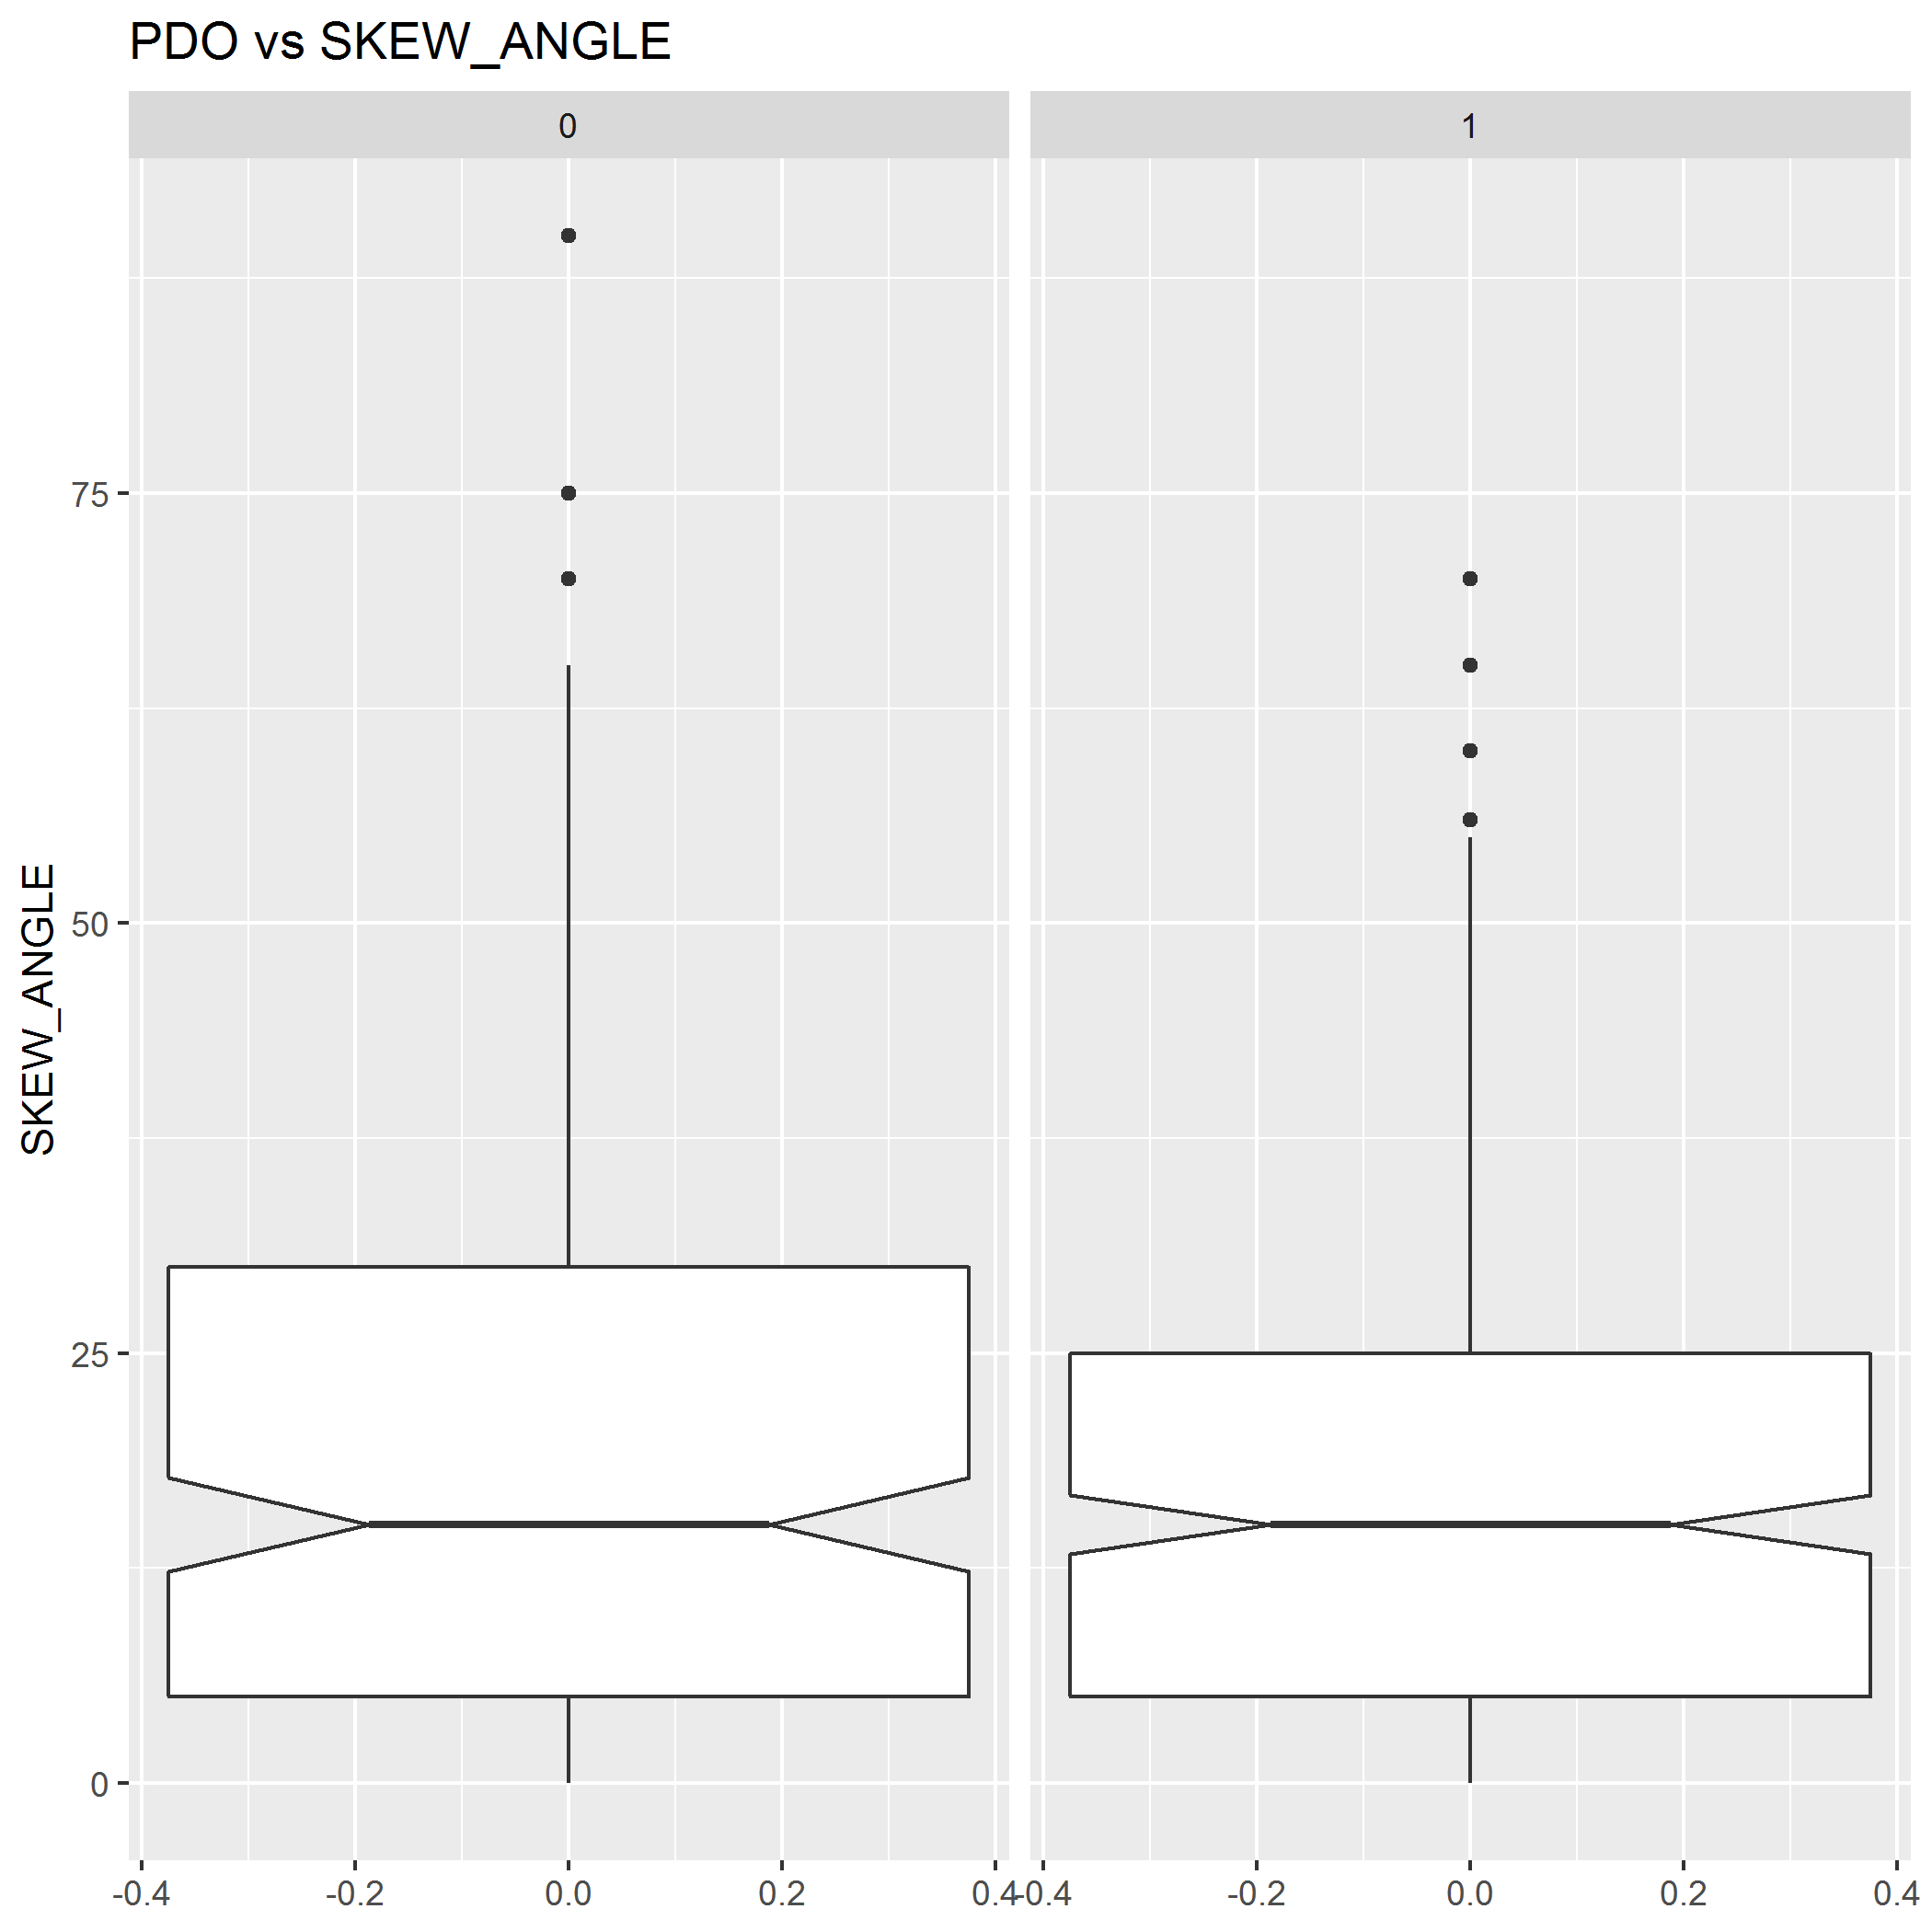
\includegraphics[width=3in]{image/angle_all_pdo.png}
\small
\end{minipage}
\begin{minipage}[t]{0.5\linewidth}
\centering
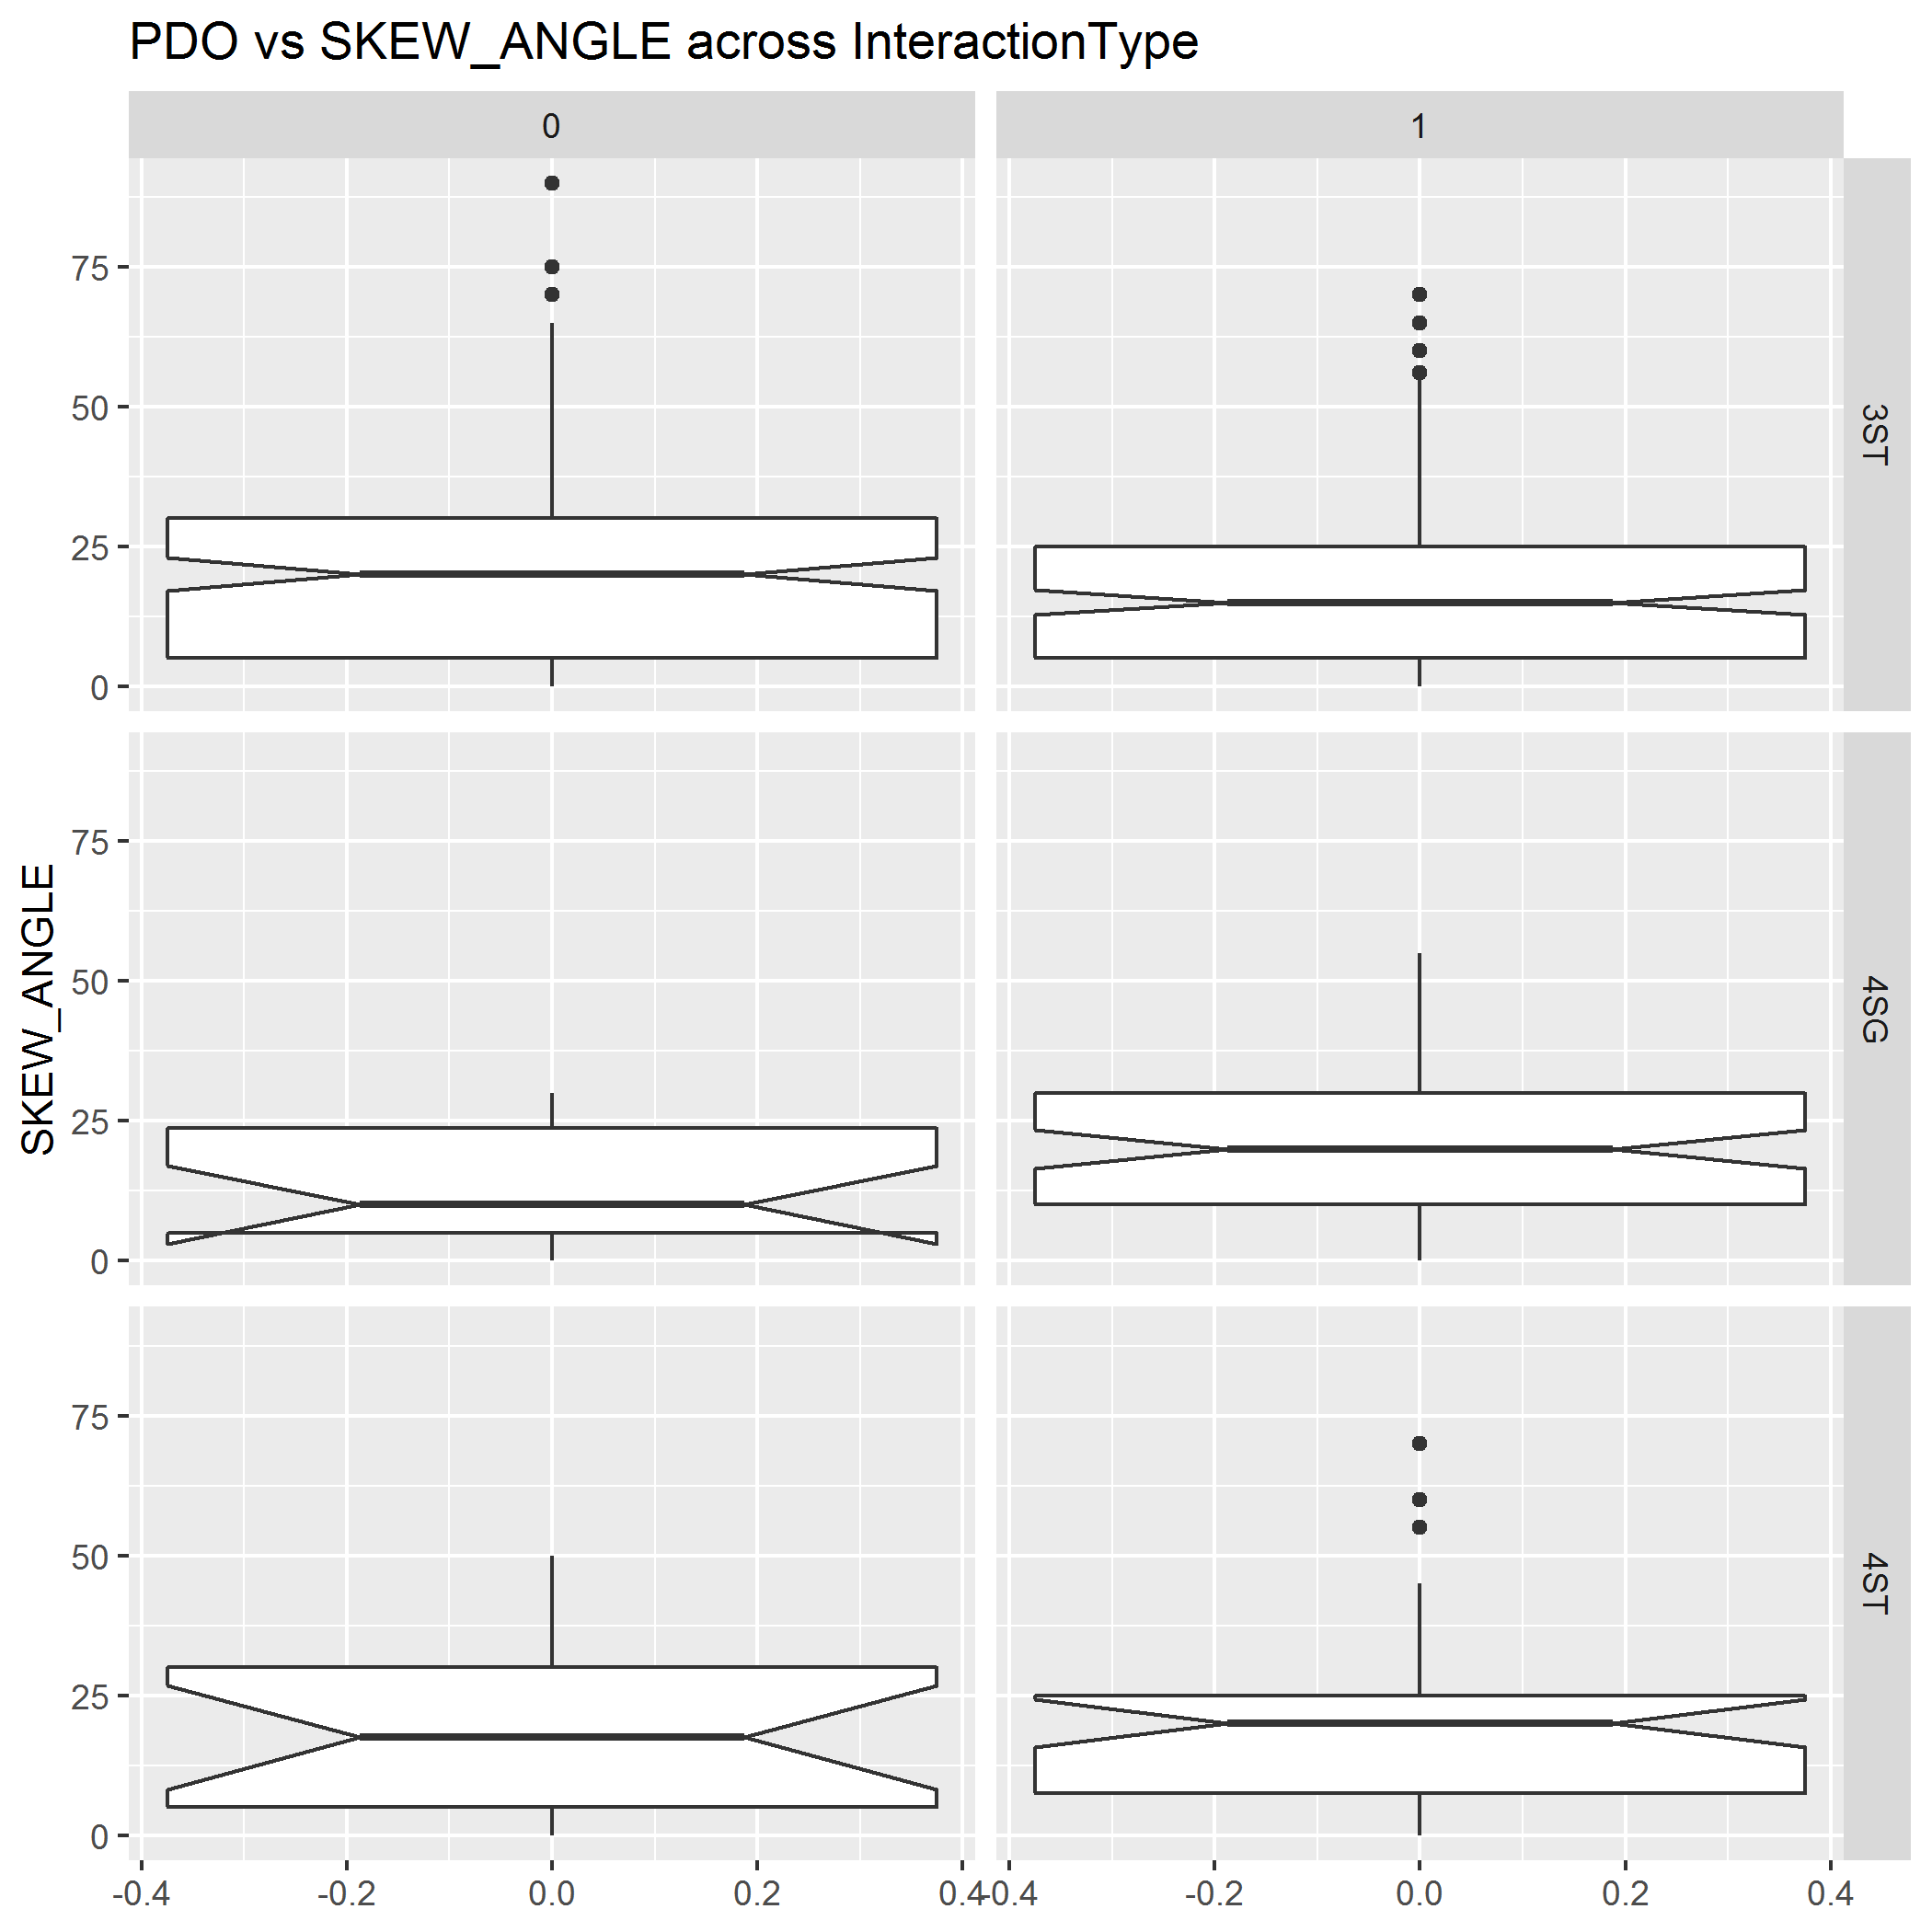
\includegraphics[width=3in]{image/angle_pdo.png}
\small
\end{minipage}
\caption{Boxplot of Skew Angle}
\end{figure}

\subsection{EDA Conclusion}

We get the following guess from the EDA part and the verification will be shown in the next inference part.

1. PDO, BC and KA has different distribution features.

2. Intersection type is a vital factor to crash counts. Four-way intersections have a higher probability for all 3 types of crash.

3. Intersection without lighting has a lower rate for all 3 types of crash. Controlling intersection type, same results are yielded except the PDO, 4ST group which has a lower crash rate when there is lighting. These results are kind of opposite to common sense.

4. Approach (left or right) turn lane has negative effect on overall crash rate, which infers that when there is an approach turn lane, the crash rate goes down. The result is reasonable only for 3ST and 4ST group individually, as 4SG group has a small number of observations.

5. AADT-Major and AADT-Minor is at a higher level in intersections with crash for whole data set. When controlling intersection, However, for AADT-Major, the tendency is only significant in 3ST group with PDO and BC. For AADT-Minor, opposite significant pattern occurs in 4SG group of PDO crash.

6. Skew angle may not act as a vital factor to crash on overall data, but may has negative effect for crash in 3ST intersections.

\section{Statistical Inference}

\subsection{One v.s. PDO crashing independence test}

We first test the relationship between crash and intersection type for 3 types of crash separately. We mainly use 3 types of methods here. When treating crash count as qualitative, normality assumption and same dispersion assumption are checked in each paired sample. Since none of the pairs satisfies normal assumption, we use Mann-Whitney test when paired sample has same dispersion. When we get different dispersion, we calculate Bootstrap confidence interval for difference of sample mean to check whether the interval contains 0 or not. If the interval contains 0, we infer that there is not obvious difference on the sample mean. (Since there is still randomness in Bootstrap, the Bootstrap CI cannot be related to test significance seriously.) Re-sampling time is set as 1000 in Bootstrap method. The same dispersion tests are carried out by Ansari-Bradley nonparametric test here. Whether the impact is positive or negative can be directly get from the tests above.

When treating turning crash counts into binary variable as 1: crash, 0: nocrash, Pearson Chi-square test is applied to check independence.

For Intersection Type vs PDO crash, only the 4ST vs 4SG group pass the same dispersion test. For 3ST vs 4ST and 3ST vs 4SG, 95\% Bootstrap Confidence Interval of difference of sample mean is calculate instead of testing. The result is shown in the table below. It infers that there is strong evidence that 4SG intersections have more PDO crash than 3ST. 4ST also has a higher level of crash than 3ST but not that strong.

\begin{table}[H]
\caption{Bootstrap Confidence Interval for PDO crash counts mean difference}
\centering
\begin{tabular}{|c|c|c|c|}
\hline
Difference of Mean  & Lower Bound & Upper Bound & Contain 0 \\
\hline
3ST-4ST & -1.652 & -0.019 & F(not obvious) \\
\hline
3ST-4SG   & -6.670  & -4.112  & F \\
\hline
\end{tabular}
\end{table}

Although some of the paired does not pass same dispersion test, we still conduct the Mann-Whitney tests on all pairs to see the results. the test may lose some power when the assumptions are violated. The test procedure is listed below. For two data sequence ${X_A}$ and ${X_B}$, the null hypothesis and alternative will be

\begin{equation*}
\begin{array}{l}
{H_0}:{q_A} = {q_B}\\
{H_1}:{q_A} > {q_B}\begin{array}{*{20}{c}}
{or}&{{q_B} > {q_A}}
\end{array}
\end{array}
\end{equation*}


where $q$ is the median, and the statistic will be

\begin{equation}
\frac{{W - E\left( W \right)}}{{\sqrt {Var\left( W \right)} }}
\end{equation}

where

\begin{equation}
\label{mw-stat}
\begin{array}{l}
W = \sum\limits_{j = 1}^n {{R_j}} \\
E\left( W \right) = \frac{{n\left( {n + m + 1} \right)}}{2}\\
Var\left( W \right) = \frac{{mn}}{{12}}\left\{ {\left( {n + m + 1} \right) - \frac{1}{{\left( {m + n} \right)\left( {m + n - 1} \right)}}\sum\limits_{j = 1}^g {{t_j}\left( {t_j^2 - 1} \right)} } \right\}
\end{array}
\end{equation}


\par

For PDO crashing between 3ST intersections and 4ST intersections, the ${q_A}$ represents the median PDO crashing for 3ST intersections, AND $q_B$ represents the median PDO crashing for 4ST intersections. Plus, in the statistic, $n$ is PDO crashing sample size for 4ST intersection; $m$ is PDO crashing sample size for 3ST intersection; $R_j$ is the $j-$th sample rank for PDO crashing rank of 4ST intersection samples; $g$ is the tie group numbers and $t_j$ is the tie group size for $j-$th tie group. According to the code in Appendix 2, our conclusion is ${{q_B} > {q_A}}$, i.e. the 4ST intersection is more likely to happen PDO crash than 3ST intersection.

\par

For PDO crashing between 4ST intersections and 4ST intersections, which the paired sample pass the same dispersion test, the ${q_A}$ represents the median PDO crashing for 4ST intersections, $q_B$ represents the median PDO crashing for 4SG intersections. Plus, in the statistic, $n$ is PDO crashing sample size for 4SG intersection; $m$ is PDO crashing sample size for 4ST intersection; $R_j$ is the $j-$th sample rank for PDO crashing rank of 4SG intersection samples; $g$ is the tie group numbers and $t_j$ is the tie group size for $j-$th tie group. According to the code in Appendix 2, our conclusion is ${{q_B} > {q_A}}$, i.e. the 4SG intersection is more likely to happen PDO crash than 4ST intersection.

\par

For PDO crashing between 3ST intersections and 4SG intersections, and the ${q_A}$ represents the median PDO crashing for 3ST intersections, $q_B$ represents the median PDO crashing for 4SG intersections. Plus, in the statistic, $n$ is PDO crashing sample size for 4SG intersection; $m$ is PDO crashing sample size for 3ST intersection; $R_j$ is the $j-$th sample rank for PDO crashing rank of 4SG intersection samples; $g$ is the tie group numbers and $t_j$ is the tie group size for $j-$th tie group. According to the code in Appendix 2, our conclusion is ${{q_B} > {q_A}}$, i.e. the 4SG intersection is more likely to happen PDO crash than 3ST intersection.

\par

According to the conclusions above, we have:

\begin{equation*}
{q_A} < {q_B} < {q_C}
\end{equation*}
where $q_A$ represents the median number of PDO crashes of 3ST intersection, $q_B$ represents the median number of PDO crashes of 4ST intersection, $q_C$ represents the median number of PDO crashes of 4ST intersection.

\par
We can use another method - Pearson test in categorical analysis - to analyze this dependence. We fistly, transform the PDO crashing number into dummy variable. If the crashing number equals to 0, then we denote it as "noncrash", while if the crashing number is greater than 0, then we denote it as "crash". Thus, we can form the following table:

\begin{table}[H]
\caption{Intersection VS Crash}
\centering
\begin{tabular}{|c|c|c|c|c|}
\hline
      & 3ST & 4ST & 4SG & Total \\
\hline
Nocrash & 173 & 18  & 18 & 209 \\
\hline
Crash    & 212  & 43  & 84  & 339 \\
\hline
Total    & 385  & 61  & 102  & 548 \\
\hline
\end{tabular}
\end{table}

Then our hypothesis will be

\begin{equation*}
\begin{array}{l}
{H_0}:{p_{ij}} = {p_i}{p_j}\\
{H_1}:{p_{ij}} \ne {p_i}{p_j}
\end{array}
\end{equation*}

and our statistic is:

\begin{equation*}
{Q_P} = \frac{{\sum\limits_{i = 1}^2 {\sum\limits_{j = 1}^3 {{{\left( {{n_{ij}} - {n_{i \cdot }}{n_{ \cdot j}}/n} \right)}^2}} } }}{{{n_{i \cdot }}{n_{ \cdot j}}/n}}
\end{equation*}

and it approximately obeys a ${\chi ^2}\left( 1 \right)$ distribution. Thus, according to the code in Appendix 2, our conclusion is: they are dependence.

\subsection{One v.s. BC and KA crashing independence test}

We next conduct the independence test for BC crashes and KA crashes similar with the way we conduct for PDO test, so the testing procedures are omitted (codes are in Appendix 2).

For 3 paired sample in KA crash, none of the pairs pass the Ansari-Bradley test. Hence, we construct Bootstrap Confidence Interval here.

\begin{table}[H]
\caption{Bootstrap Confidence Interval for KA crash counts mean difference}
\centering
\begin{tabular}{|c|c|c|c|}
\hline
Difference of Mean  & Lower Bound & Upper Bound & Contain 0 \\
\hline
3ST-4ST & -1.180 & 0.014 & Y(not obvious) \\
\hline
3ST-4SG   & -0.267  & -0.078  & F(not obvious) \\
\hline
4ST-4SG   & -0.209  & 0.047 & Y(not obvious) \\
\hline
\end{tabular}
\end{table}

For 3 paired sample in BC crash, none of the pairs pass the Ansari-Bradley test. Hence, we also construct Bootstrap Confidence Interval here.

\begin{table}[H]
\caption{Bootstrap Confidence Interval for BC crash counts mean difference}
\centering
\begin{tabular}{|c|c|c|c|}
\hline
Difference of Mean  & Lower Bound & Upper Bound & Contain 0 \\
\hline
3ST-4ST & -0.716 & 0.070 & Y(not obvious) \\
\hline
3ST-4SG   & -2.376  & -1.361  & F \\
\hline
4ST-4SG   & -2.164  & -0.930 & F \\
\hline
\end{tabular}
\end{table}

The Mann Whitney tests are still done and generate the result below. The order of median is the same as the shown in the Bootstrap confidence interval. However, the Bootstrap interval show some evidence that some of the inequality signs are not strictly holds.

\begin{itemize}
	\item ${q_A} < {q_B} < {q_C}$, where $q_A$ represents the median number of BC crashes of 3st intersection, $q_B$ represents the median number of BC crashes of 4st intersection, $q_C$ represents the median number of BC crashes of 4sg intersection.
	\item ${q_A} < {q_B} = {q_C}$, where $q_A$ represents the median number of KA crashes of 3st intersection, $q_B$ represents the median number of KA crashes of 4st intersection, $q_C$ represents the median number of KA crashes of 4sg intersection.
\end{itemize}

The Pearson tests are also applied. And finally both of these two Pearson tests show dependence. Two categorical tables are:

\begin{table}[H]
\caption{Categorical table for BC crash}
\centering
\begin{tabular}{|c|c|c|c|c|}
\hline
      & 3ST & 4ST & 4SG & Total \\
\hline
Nocrash & 264 & 31  & 30 & 325 \\
\hline
Crash    & 121  & 30  & 72  & 223 \\
\hline
Total    & 385  & 61  & 102  & 548 \\
\hline
\end{tabular}
\end{table}

\begin{table}[H]
\caption{Categorical table for KA crash}
\centering
\begin{tabular}{|c|c|c|c|c|}
\hline
      & 3ST & 4ST & 4SG & Total \\
\hline
Nocrash & 370 & 55  & 83 & 508 \\
\hline
Crash    & 15  & 6  & 19  & 50 \\
\hline
Total    & 385  & 61  & 102  & 548 \\
\hline
\end{tabular}
\end{table}

From the discussion between intersection type and crash counts, we can draw the follow conclusion:

(1) There are dependent between intersection type and crash counts for all 3 types of crashes by Pearson tests.

(2) By Mann-whitney test, for PDO, 4SG intersection is more likely to happen PDO crash than 4ST intersection.

(3) As there is still randomness in Bootstrap method, some intervals constructed above have bounds close to 0, which may change sign in other realizations. Hence, here we take |x|>0.1 as an obvious difference from 0. From the tables above and combine with Mann-whitney test results, we can claim that for PDO, 4SG has obvious more crash than 3ST; for BC, 4SG has obvious more crash than 3ST and 4ST; for KA, there is likely to be no obvious pattern. However, all intervals constructed have the tendency to be at the left side of 0, which infers that there might be a tendency that the unit number of crash in all 3 types of crash follow the order 3ST<4ST<4SG.

\subsection{Two v.s. crashing independence test}

\subsubsection{Crossing type + Skewed Angle v.s. Crashing}

As we the skewed angle holds little choices of values, we decide to transform skewed angle into categorical data and also transform PDO crashing number as our previous method, forming the categorical table below. We settle a standard: let $s$ denote the skewed angle, if $0 \le s \le 30$, then we record it as ``1''; If $31 \le s \le 60$, then we record it as ``2''; If $61 \le s \le 90$, then we record it as ``3''. The effect is tested with interaction category across intersection types and skew angle. The 2-by-n tables are shown below.

\begin{table}[H]
\caption{Discrete skew v.s. PDO crash}
\centering
\begin{tabular}{|c|c|c|c|c|c|c|c|c|c|}
\hline
      & 3ST\_1 & 3ST\_2 & 3ST\_3 & 4ST\_1 & 4ST\_2 & 4ST\_3 & 4SG\_1 & 4SG\_2 & Total \\
\hline
Nocrash & 131 & 31  & 11 & 14 & 4 & 0 & 18 & 0 & 209\\
\hline
Crash    & 168  & 39  & 5  & 36 & 6 & 1 & 71 & 13 & 339\\
\hline
Total    & 299  & 70  & 16  & 50 & 10 & 1 & 89 & 13 & 548 \\
\hline
\end{tabular}
\end{table}

\begin{table}[H]
\caption{Discrete skew v.s. BC crash}
\centering
\begin{tabular}{|c|c|c|c|c|c|c|c|c|c|}
\hline
      & 3ST\_1 & 3ST\_2 & 3ST\_3 & 4ST\_1 & 4ST\_2 & 4ST\_3 & 4SG\_1 & 4SG\_2 & Total \\
\hline
Nocrash & 203 & 46  & 15 & 25 & 6 & 0 &  29 & 1 & 325\\
\hline
Crash    & 96  & 24  & 1  &  25 & 4 & 1 & 60 & 12 & 223\\
\hline
Total    & 299  & 70  & 16  & 50 & 10 & 1 & 89 & 13 & 548 \\
\hline
\end{tabular}
\end{table}

\begin{table}[H]
\caption{Discrete skew v.s. KA crash}
\centering
\begin{tabular}{|c|c|c|c|c|c|c|c|c|c|}
\hline
      & 3ST\_1 & 3ST\_2 & 3ST\_3 & 4ST\_1 & 4ST\_2 & 4ST\_3 & 4SG\_1 & 4SG\_2 & Total \\
\hline
Nocrash &  285  & 69  & 16 & 44 & 10 &  1 &  71 & 12 &  508\\
\hline
Crash    & 14  & 1  & 0  &  6 & 0 & 0 & 18 & 1 & 40\\
\hline
Total    & 299  & 70  & 16  & 50 & 10 & 1 & 89 & 13 & 548 \\
\hline
\end{tabular}
\end{table}

Then, the Pearson test shows that there exists a dependence for all three kinds of crashes (codes are in Appendix 2.) and we have also conducted the association test for separate single one vs one group as following, the p-value table shows:

\begin{table}[H]
\caption{P-value for skew angle vs Crash}
\centering
\begin{tabular}{|c|c|c|c|c|c|c|c|c|c|}
\hline
p-value & 3ST & 4ST & 4SG  \\
\hline
PDO & 0.1472 & 0.6058 & 0.2026 \\
\hline
BC & 0.0806 & 0.5006 & 0.1840\\
\hline
KA & 0.3197  & 0.4809 & 0.5556 \\
\hline
Mixed & 0.0496 & 0.2618 & 0.2026 \\
\hline
\end{tabular}
\end{table}

The one vs one test show no significance except 3ST with mixed data, which is opposite to the overall test.


\subsubsection{Crossing type + Lighting vs Crashing}

As the lighting itself is a dummy variable, we can form the following categorical table:

\begin{table}[H]
\caption{Crossing type + Lighting v.s. PDO crash}
\centering
\begin{tabular}{|c|c|c|c|c|c|c|c|}
\hline
      & 3ST\_0 & 3ST\_1 & 4ST\_0 & 4ST\_1 & 4SG\_0 & 4SG\_1 & Total \\
\hline
Nocrash & 74 & 99 & 5 & 13 & 6 & 12 & 209\\
\hline
Crash    & 76  & 136  & 18 & 25 & 28 & 66 & 339\\
\hline
Total    & 150  & 235  & 23  & 38 & 24 & 78 & 548 \\
\hline
\end{tabular}
\end{table}

Then, the Pearson test shows that there exists a dependence (codes are in Appendix 2.)

One vs one tests are also done here.

We also use the three 2-by-2 contingency tables between Lighting and crash with PDO crash for each intersection type, which can directly get from table above.  Same table are generated for KA and BC. For all 2-by-2 table, only table of KA, 4ST has cell counts less than 5. For this one, we apply Fisher-exact test. For others, we conduct individual Pearson test on each table. None of the above tests reject the Null hypothesis. P-value are shown in table below. When testing the overall effect across table, in the Mantel-Haenszel test cannot reject the Null in all 3 types of crashes. Hence, no dependence of Lighting and crash are observed here.

When we mix 3 types of crash together and still construct 2-by-2 table across intersections, same results are generated.

In all, we conclude that there is no effect of Lighting on crash when controlling intersection type.

\begin{table}[H]
\caption{P-value for Lighting vs Crash}
\centering
\begin{tabular}{|c|c|c|c|c|c|c|c|c|c|}
\hline
p-value & 3ST & 4ST & 4SG  \\
\hline
PDO & 0.1657 & 0.3006 & 0.7644 \\
\hline
KA & 0.6484 & 0.0746 & 0.7509\\
\hline
BC & 0.247  & 0.4883 & 0.976 \\
\hline
Mixed & 0.0879 & 0.9494 & 0.5732 \\
\hline
\end{tabular}
\end{table}

Again,the one vs one test show opposite result to the overall test.

\subsubsection{Crossing type + turns for Turn vs Crashing}

Based on the results from the EDA part, we combine Approach Left Turn and Approach Right Turn as one dummy variable where 1 stands for there is an approach turn and 0 stands for not. Even then, approach turn existence is still a rare event in all intersection types.  Also, if we continuing partitioning the data by crash type to form contingency table, we will have cells with extremely small counts equal to 0. Hence, we only analyses with mixed data with all crashes types mixed. We can form the following contingency table:

\begin{table}[H]
\caption{Overall Crossing type + turns v.s. crash}
\centering
\tiny
\begin{tabular}{|c|c|c|c|c|c|c|c|c|c|c|c|c|}
\hline
      & 3ST\_00 & 3ST\_01 & 3ST\_10 & 3ST\_11 & 4ST\_00 & 4ST\_10 & 4ST\_11 & 4SG\_00 & 4SG\_01 & 4SG\_10 & 4SG\_11 & Total \\
\hline
Nocrash & 164  & 2 & 3 & 4 & 18 & 0 & 0 & 9 & 1 & 4 & 4 & 209\\
\hline
Crash   & 200  & 2 & 7 & 3 & 39 & 3 & 1 & 46 & 2 & 18 & 18 & 339 \\
\hline
Total   & 364  & 4 & 10 & 7 & 57 & 3 & 1 & 55 & 3 & 22 & 22 & 548\\
\hline
\end{tabular}
\end{table}

where ``00'' represents no left approach or right approach; ``01'' represents no left approach but a right approach; ``10'' represents no right approach but left approach; ``11'' represents a left approach and right approach. Then, the Pearson test shows that there exists a dependence (codes are in Appendix 2.)

One vs one tests are also applied with 2-by-2 tables from above larger table for each intersection type separately. We do both Mantel-Haenszel test and 3 individual tests to test for independence between column and row.

For the 3 individual test, for 3ST and 4SG, we have all cell counts larger than 5. We apply Pearson Chi-square tests and get p-value as 0.7834 and 0.713, which infers there is no dependency. For 4ST, we use the Fisher-exact test as counts are rather small and get p-value of 0.3729. The individual tests show no relationship between Crash and Turns.

For the Mantel-Haenszel test, although we get the result that there is no overall effect of Turn on crash when controlling intersection type, the assumptions are not all satisfied due to small cell counts. But, it can still be some kind of evidence that there is no relationship.

Again, we get difference result between overall test and one vs one test.

\subsubsection{Crossing type + AADT major VS Crashing}

We firstly partition the full samples into 6 parts: 3ST intersection + crash; 3ST intersection + noncrash; 4ST intersection + crash; 4ST intersection + noncrash; 4SG intersection + crash; 4SG intersection + noncrash. And we carry out a Shapiro normality test on these 6 sample pieces, however, few of them pass the test. Hence, once again, we need to turn to the Mann-Whitney test.

\par

Comparing the AADT major and controlling the intersection type in 3st, we have the following hypotheses:

\begin{equation*}
\begin{array}{l}
{H_0}:{q_A} = {q_B}\\
{H_1}:{q_A} < {q_B}\begin{array}{*{20}{c}}
{or}&{{q_A} > {q_B}}
\end{array}
\end{array}
\end{equation*}

where $q_A$ represents the median of AADT major in PDO noncrash situation in 3ST intersection, while $q_B$ represents the median of AADT major with PDO crash situation in 3ST intersection. And the statistic is similar with \eqref{mw-stat}. And our final conclusion (codes are in Appendix 2) is:

\begin{equation*}
{q_A} < {q_B}.
\end{equation*}

\par

Comparing the AADT major and controlling the intersection type in 4ST, we have the following hypotheses:

\begin{equation*}
\begin{array}{l}
{H_0}:{q_A} = {q_B}\\
{H_1}:{q_A} < {q_B}\begin{array}{*{20}{c}}
{or}&{{q_A} > {q_B}}
\end{array}
\end{array}
\end{equation*}

where $q_A$ represents the median of AADT major in PDO noncrash situation in 4ST intersection, while $q_B$ represents the median of AADT major with PDO crash situation in 4ST intersection. And the statistic is similar with \eqref{mw-stat}. And our final conclusion (codes are in Appendix 2) is:

\begin{equation*}
{q_A} = {q_B}.
\end{equation*}

\par

Comparing the AADT major and controlling the intersection type in 4SG, we have the following hypotheses:

\begin{equation*}
\begin{array}{l}
{H_0}:{q_A} = {q_B}\\
{H_1}:{q_A} < {q_B}\begin{array}{*{20}{c}}
{or}&{{q_A} > {q_B}}
\end{array}
\end{array}
\end{equation*}

where $q_A$ represents the median of AADT major in PDO noncrash situation in 4SG intersection , while $q_B$ represents the median of AADT major with PDO crash situation in 4SG intersection. And the statistic is similar with \eqref{mw-stat}. And our final conclusion (codes are in Appendix 2) is:

\begin{equation*}
{q_A} = {q_B}.
\end{equation*}

By same Mann-Whitney tests, for KA crash, AADT-Major only has significant effect at 3ST intersection. Larger AADT-Major intersection has higher crash rate. For BC crash, significant impact is observed both in 3ST and 4ST. In both case, larger AADT-Major is related to higher crash rate.

\subsubsection{Crossing type + AADT minor vs Crashing}

With the same partition made for AADT major,we also carry out a Shapiro normality test on these 6 sample pieces for AADT minor, however, few of them pass the test. Hence, once again, we need to turn to the Mann-Whitney test.

\par

Comparing the AADT minor and controlling the intersection type in 3ST, we have the following hypotheses:

\begin{equation*}
\begin{array}{l}
{H_0}:{q_A} = {q_B}\\
{H_1}:{q_A} < {q_B}\begin{array}{*{20}{c}}
{or}&{{q_A} > {q_B}}
\end{array}
\end{array}
\end{equation*}

where $q_A$ represents the median of AADT minor in PDO noncrash situation in 3st intersection, while $q_B$ represents the median of AADT minor with PDO crash situation in 3ST intersection. And the statistic is similar with \eqref{mw-stat}. And our final conclusion (codes are in Appendix 2) is:

\begin{equation*}
{q_A} < {q_B}.
\end{equation*}

\par

Comparing the AADT minor and controlling the intersection type in 4ST, we have the following hypotheses:

\begin{equation*}
\begin{array}{l}
{H_0}:{q_A} = {q_B}\\
{H_1}:{q_A} < {q_B}\begin{array}{*{20}{c}}
{or}&{{q_A} > {q_B}}
\end{array}
\end{array}
\end{equation*}

where $q_A$ represents the median of AADT minor in PDO noncrash situation in 4ST intersection, while $q_B$ represents the median of AADT minor with PDO crash situation in 4ST intersection. And the statistic is similar with \eqref{mw-stat}. And our final conclusion (codes are in Appendix 2) is:

\begin{equation*}
{q_A} = {q_B}.
\end{equation*}

\par

Comparing the AADT minor and controlling the intersection type in 4SG, we have the following hypotheses:

\begin{equation*}
\begin{array}{l}
{H_0}:{q_A} = {q_B}\\
{H_1}:{q_A} < {q_B}\begin{array}{*{20}{c}}
{or}&{{q_A} > {q_B}}
\end{array}
\end{array}
\end{equation*}

where $q_A$ represents the median of AADT minor in PDO noncrash situation in 4SG intersection , while $q_B$ represents the median of AADT minor with PDO crash situation in 4SG intersection. And the statistic is similar with \eqref{mw-stat}. And our final conclusion (codes are in Appendix 2) is:

\begin{equation*}
{q_A} = {q_B}.
\end{equation*}

By same Mann-Whitney tests, for KA crash, no significant effects is observed. For BC crash, positive effect on crash rate is observed in 3ST intersection. For 4ST group, the AADT-Minor in crash and noncrash group do not pass the same dispersion test. We again carry out the Bootstrap Confidence Interval method on the difference of sample mean. The 95\% interval for mean(crash)-mean(noncrash) is (100,1051.25). Hence, there is obvious positive effect of AADT-Minor on crash rate in 4ST.

\section{Discussion of Results and Concluding Remarks}

\subsection{Conclusions}

From all the discussion above, we can draw the conclusion below:

For Intersection Type vs crash counts only: Intersection type affects the probability of all 3 types of crash. There is a tendency that the crash probability in 3 types of intersection follows that order 3ST<4ST<4SG. The tendency is obvious in PDO,4SG vs 4ST and BC, 3ST vs 4ST vs 4SG. We may recommend to pay much more attention when coming across a 4SG intersection.

Controlling intersection type:

(1) Skew angle and Lighting: The effect of skew angle is not significant when controlling intersection type, while the interaction effect between intersection and skew angle is tested to be significant.

(2) Turns: Discussions only focus on data with 3 types of crashes mixed together due to lack of observations. Again, we have insignificant effect of turns with significant interaction effect between turns and intersection types.

(3) AADT-Major and AADT-Minor: Only positive impact of AADT-Major and AADT-Minor is observed on crash rate. For PDO, 3ST intersection with higher AADT-Major level or higher AADT-Minor level tends to has higher crash rate. For KA, same impact observed in 3ST. For BC, such positive effect occurs in 3ST and 4ST. The result infers that controlling AADT at a lower level might be a good method to reduce crash rate at 3ST and 4ST intersection, but might not help for 4SG intersections.

The results in (1) and (2) need further discussion as the existence of contradict between main effect and interaction effect. Overall, there is no common suggestion based on skew angle, lighting and turns towards crash.


\subsection{Further Discussion}

For all the analysis above, we mainly apply 3 types of technique: data visualization, confidence interval construction and hypothesis testing on location and scale. Here are some other probable methods that can be applied to explore the data set.

\subsubsection{Logistic regression}

All the methods used can hardly predict the crash rate or crash counts. Also, the impact of certain variable when controlling 2 or more other variables cannot be discusses with current technique. Since we have counts as response variable and also many 0 in the data set, logistic models are a good option here to fit the data, either with normal family(predict crash rate) or with poisson/negative-binomial family(predict crash counts). Then we can get prediction of crash and also further explore the effect of regressors in the full model.

\subsubsection{Sufficient dimension reduction}

In statistical fields, there is a special topic - sufficient dimension reduction - which is used to select most relative variable to the response. Mathematically, for $Y$ as response and $X$ as a $p-$dimension predictor, we'd like to find a $p \times d\left( {d < p} \right)$ vector $\eta $ such that

\begin{equation*}
Y \bot X\left| {{\eta ^T}X}. \right.
\end{equation*}

where ${\eta ^T}X$ is denoted as the central subspace ${S_{Y\left| X \right.}}$. Proposed by Li et. al.\cite{li2011principal}, the principal support vector machines is a popular sufficient dimension reduction method. The estimation procedure can be divided into three steps:

\begin{itemize}
	\item 1. Compute the sample mean $\bar X$ and sample variance matrix $\hat \Sigma $.
	\item 2. (Optimization) Let ${q_r},r = 1, \ldots ,h - 1$ be $h-1$ dividing points,equally spaced sample percentiles of $\left\{ {{Y_1}, \ldots ,{Y_n}} \right\}$. Let
	\begin{equation*}
	\tilde Y_i^r = I\left( {{Y_i} > {q_r}} \right) - I\left( {{Y_i} \le {q_r}} \right).
	\end{equation*}
	Then let $\left( {{{\hat \beta }_r},{{\hat t}_r}} \right)$ be the minimizer of
	\begin{equation*}
	{\beta ^T}\hat \sum \beta  + \lambda {E_n}{\left\{ {1 - {{\tilde Y}^r}\left[ {{{\left( {X - \bar X} \right)}^T}\beta  - t} \right]} \right\}^ + }.
	\end{equation*}
	\item 3. (Estimation)  Let ${\hat v_1}, \ldots ,{\hat v_d}$ be the d leading eigenvectors of matrix
	\begin{equation*}
	{\hat M_n} = \sum\nolimits_{r = 1}^{h - 1} {{{\hat \beta }_r}\hat \beta _r^T}.
	\end{equation*}
	Then we use subspace spanned by $\hat v = \left( {{{\hat v}_1}, \ldots ,{{\hat v}_d}} \right)$ to estimate ${S_{Y\left| X \right.}}$.
\end{itemize}

By the way, proposed by Xia et. al.\cite{xia2015consistently}, the eigenvector number $d$ can be selected by the jump ratio of eigenvalues. That is, if ${\lambda _1}, \ldots ,{\lambda _p}$ is $p$ eigenvalues of the matrix in descending order, then we forming the $p-1$ jump ratio by
\begin{equation*}
\left\{ {{J_1}, \ldots ,{J_{p - 1}}} \right\},{J_i} = \frac{{{\lambda _i}}}{{{\lambda _{i + 1}}}},
\end{equation*}

then we select $d$ as

\begin{equation*}
d = \mathop {\arg \max }\limits_i {J_i}.
\end{equation*}



Geometrically, the following figure shows the principal.

\begin{figure}[H]
\centering
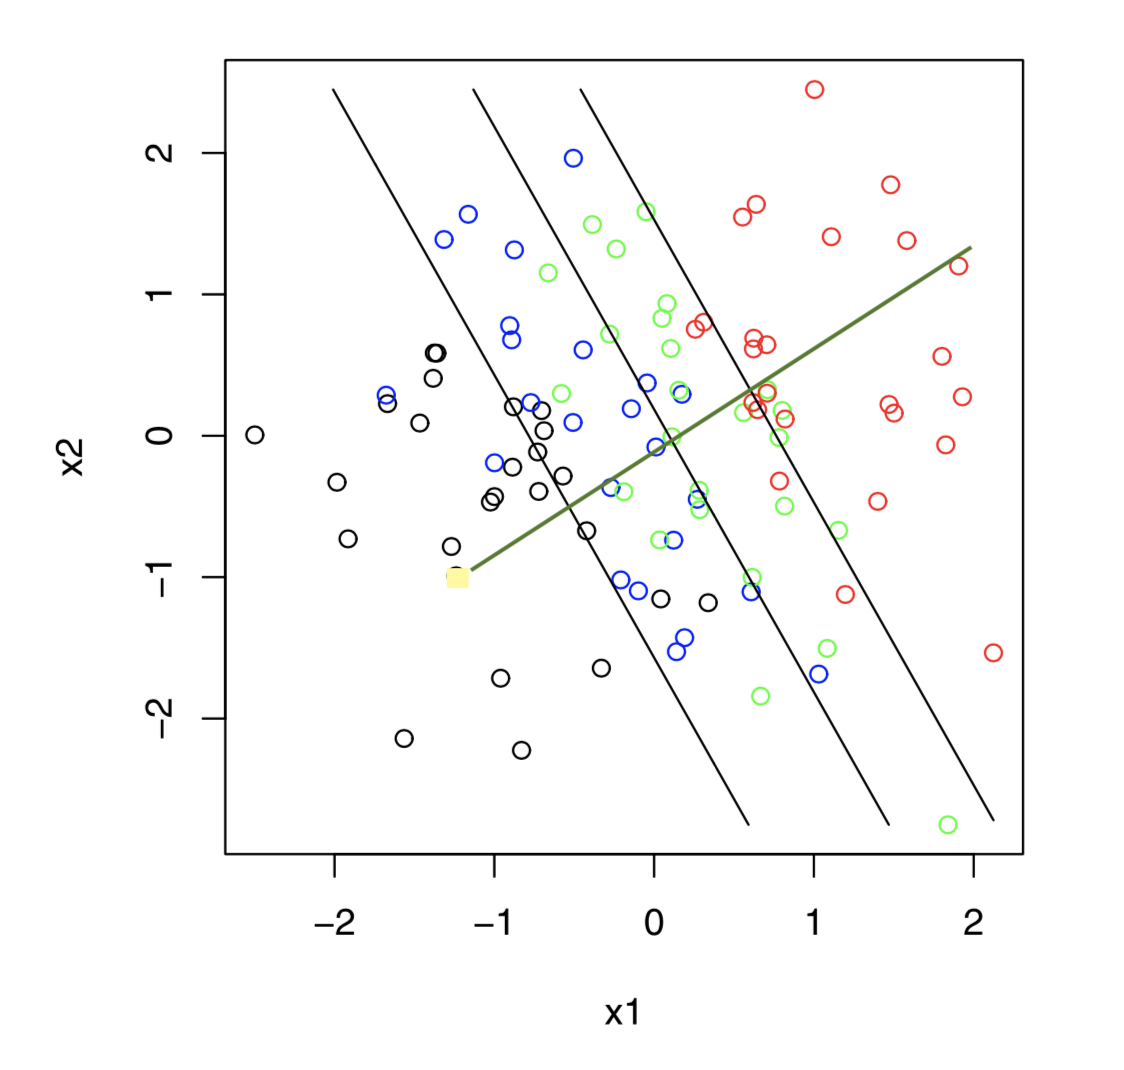
\includegraphics[width=3in]{image/psvm.png}
\small
\caption{2 dimension SVM surfaces and their normal line}
\end{figure}

In the figure, if the colors represent the value, from red (4th quantile part) to black (1st quantile part), the value $Y$ descends. Then, three black surface is the SVM boundary for its four quantile parts. Finally, the green line - the normal direction of its SVM boundary - can perfectly delineate a path (forming by the weights of $x_1$ and $x_2$) where the $Y$ value grows fastest.

\par

Implementing this algorithm by Python (code is in Appendix 2), we get the central subspace for PDO crashing number as response:

\begin{lstlisting}
array([[ 0.00000000e+00, -6.28336625e-03, -3.44987939e-04, -1.54542490e-04],
       [ 9.99807242e-01, -1.96296091e-02, -3.32648777e-04, -1.63439760e-04],
       [-9.52640689e-04, -2.96027569e-02, -9.24611159e-01, -3.78741274e-01],
       [-1.67939885e-04, -7.34446402e-03, -2.37055602e-01, 6.33323237e-01],
       [-7.19757840e-05, -6.52082837e-03, -2.96534802e-01, 6.74871829e-01],
       [ 1.96096296e-02,  9.99300962e-01, -3.10761591e-02, -2.16533571e-03]])
\end{lstlisting}

\par

It shows that for PDO crashing number, there are totally 4 factors which may significantly affects it. The AADT major holds a positive effect ( 9.99807242e-01) to PDO crash; The skewed angle holds a positve effect (9.99300962e-01) to PDO crash; The lighting holds a negative effect (-9.24611159e-01) to PDO crash; The right-turn approach holds positive effect (6.74871829e-01) to PDO crash.

\par

Similarly, for BC crashing number as response, the central subspace will be:

\begin{lstlisting}
array([[ 4.00994989e-05,  1.88638392e-05,  2.29261861e-04],
       [-2.92592349e-05, -2.48004596e-06, -4.20608685e-05],
       [-9.87266764e-01, -1.21357177e-02, -1.58483896e-01],
       [-1.53212888e-01,  3.38178083e-01,  9.28526411e-01],
       [ 4.23293850e-02,  9.41003883e-01, -3.35737815e-01],
       [-6.19423106e-03,  1.07378434e-05, -1.27455844e-03]])
\end{lstlisting}

It can also reveal three key and relative factor: lighting for negative effect, left-turn and right-turn approaches for positive effect. And certainly we can do the same procedure on the KA crashing easily, so we omit it here.

\section{Appendix}

\subsection{Extra Plots}

Extra support plots for AADT-Major:

\begin{figure}[H]
\begin{minipage}[t]{0.5\linewidth}
\centering
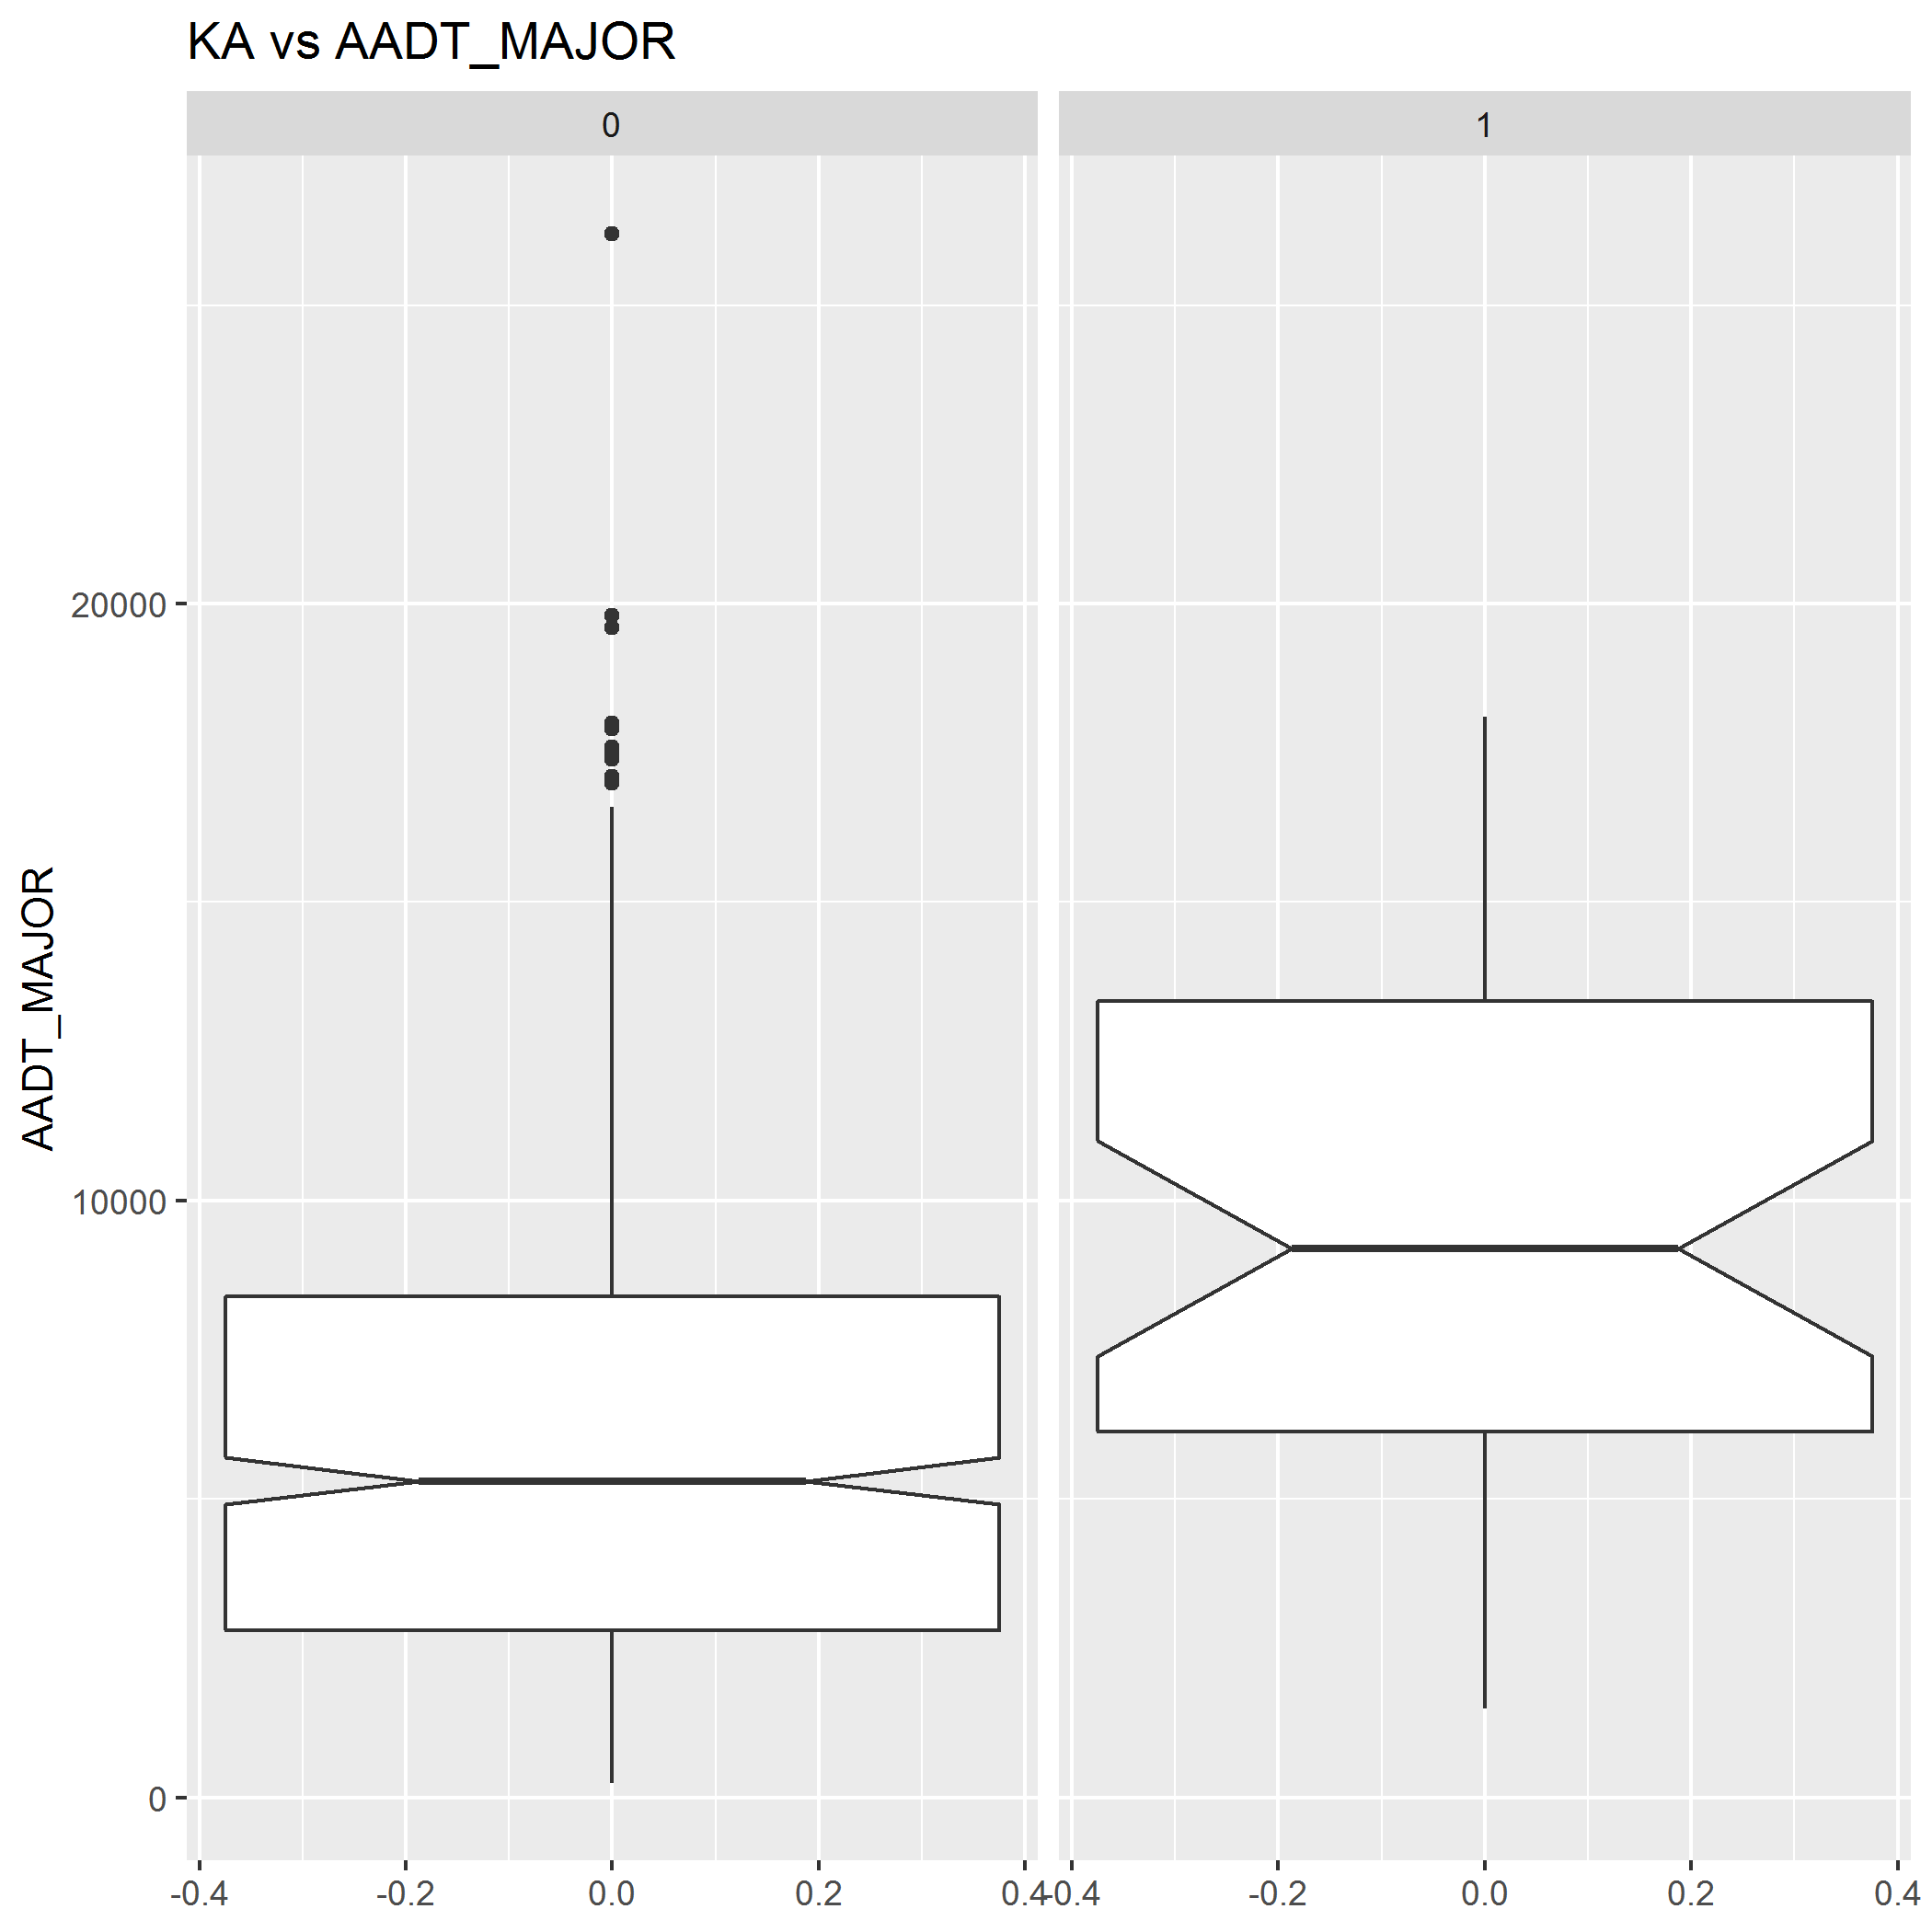
\includegraphics[width=3in]{image/extra1.png}
\small
\end{minipage}
\begin{minipage}[t]{0.5\linewidth}
\centering
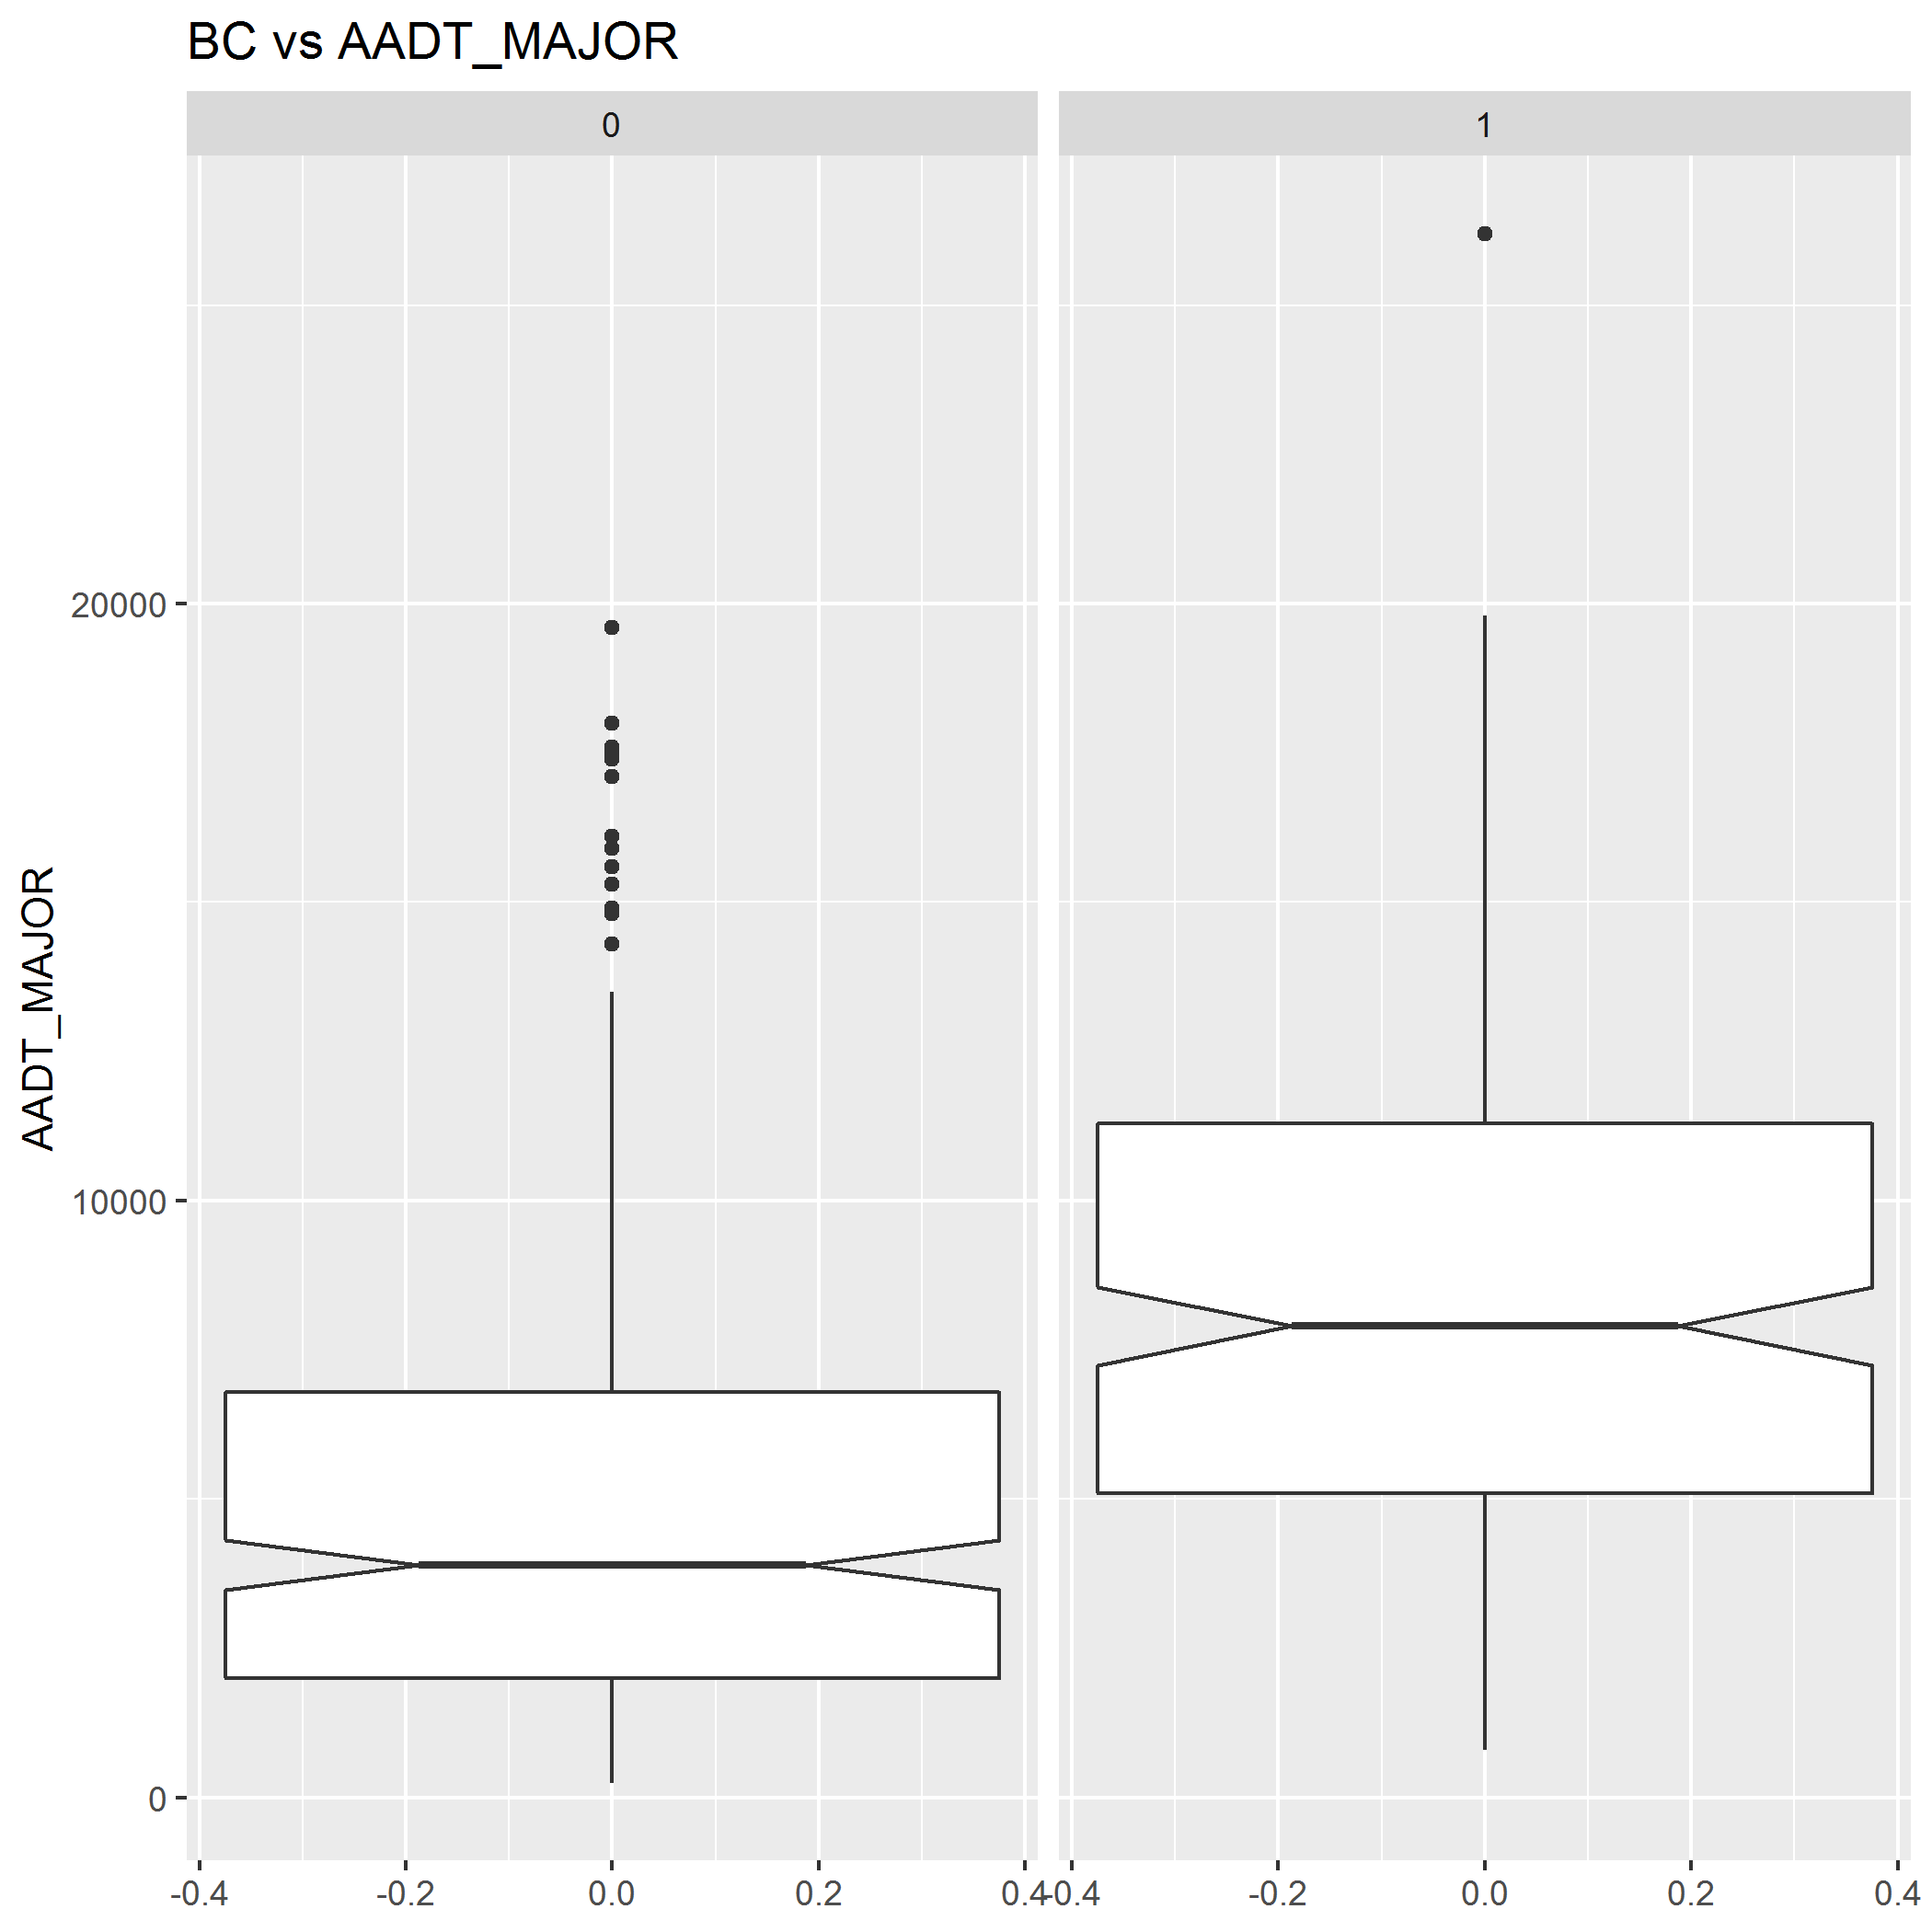
\includegraphics[width=3in]{image/extra2.png}
\small
\end{minipage}
\begin{minipage}[t]{0.5\linewidth}
\centering
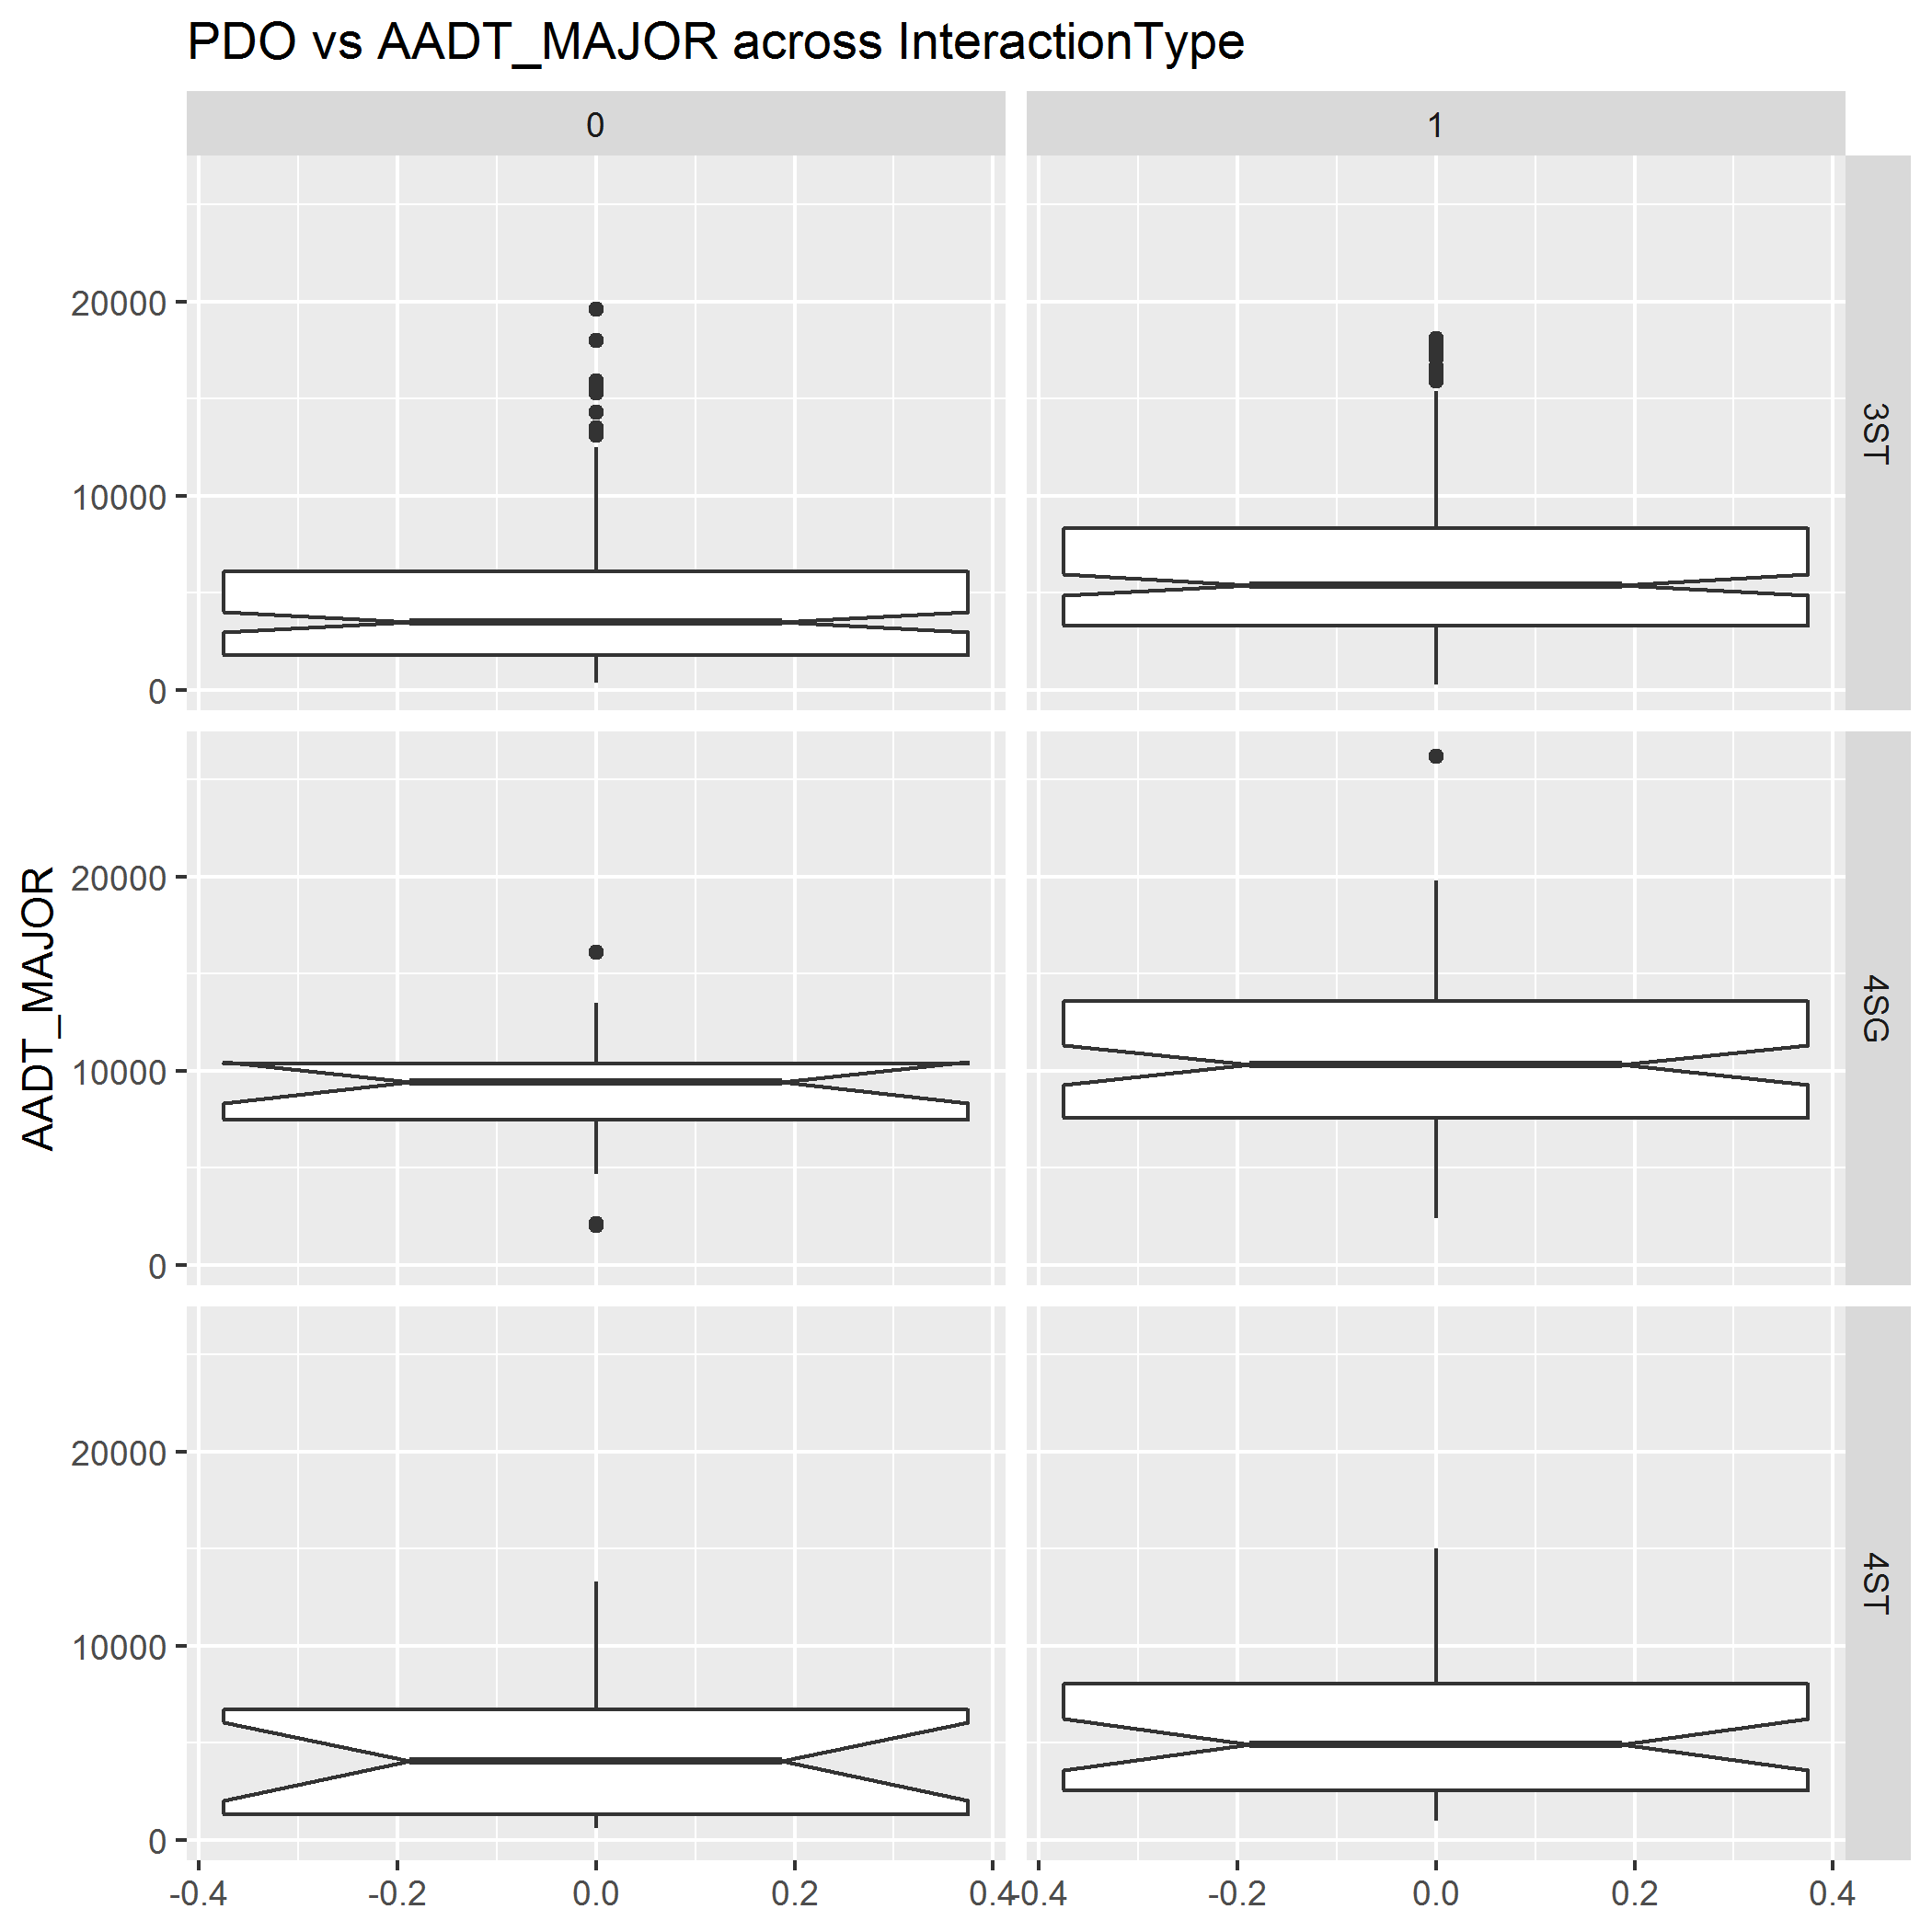
\includegraphics[width=3in]{image/extra3.png}
\small
\end{minipage}
\begin{minipage}[t]{0.5\linewidth}
\centering
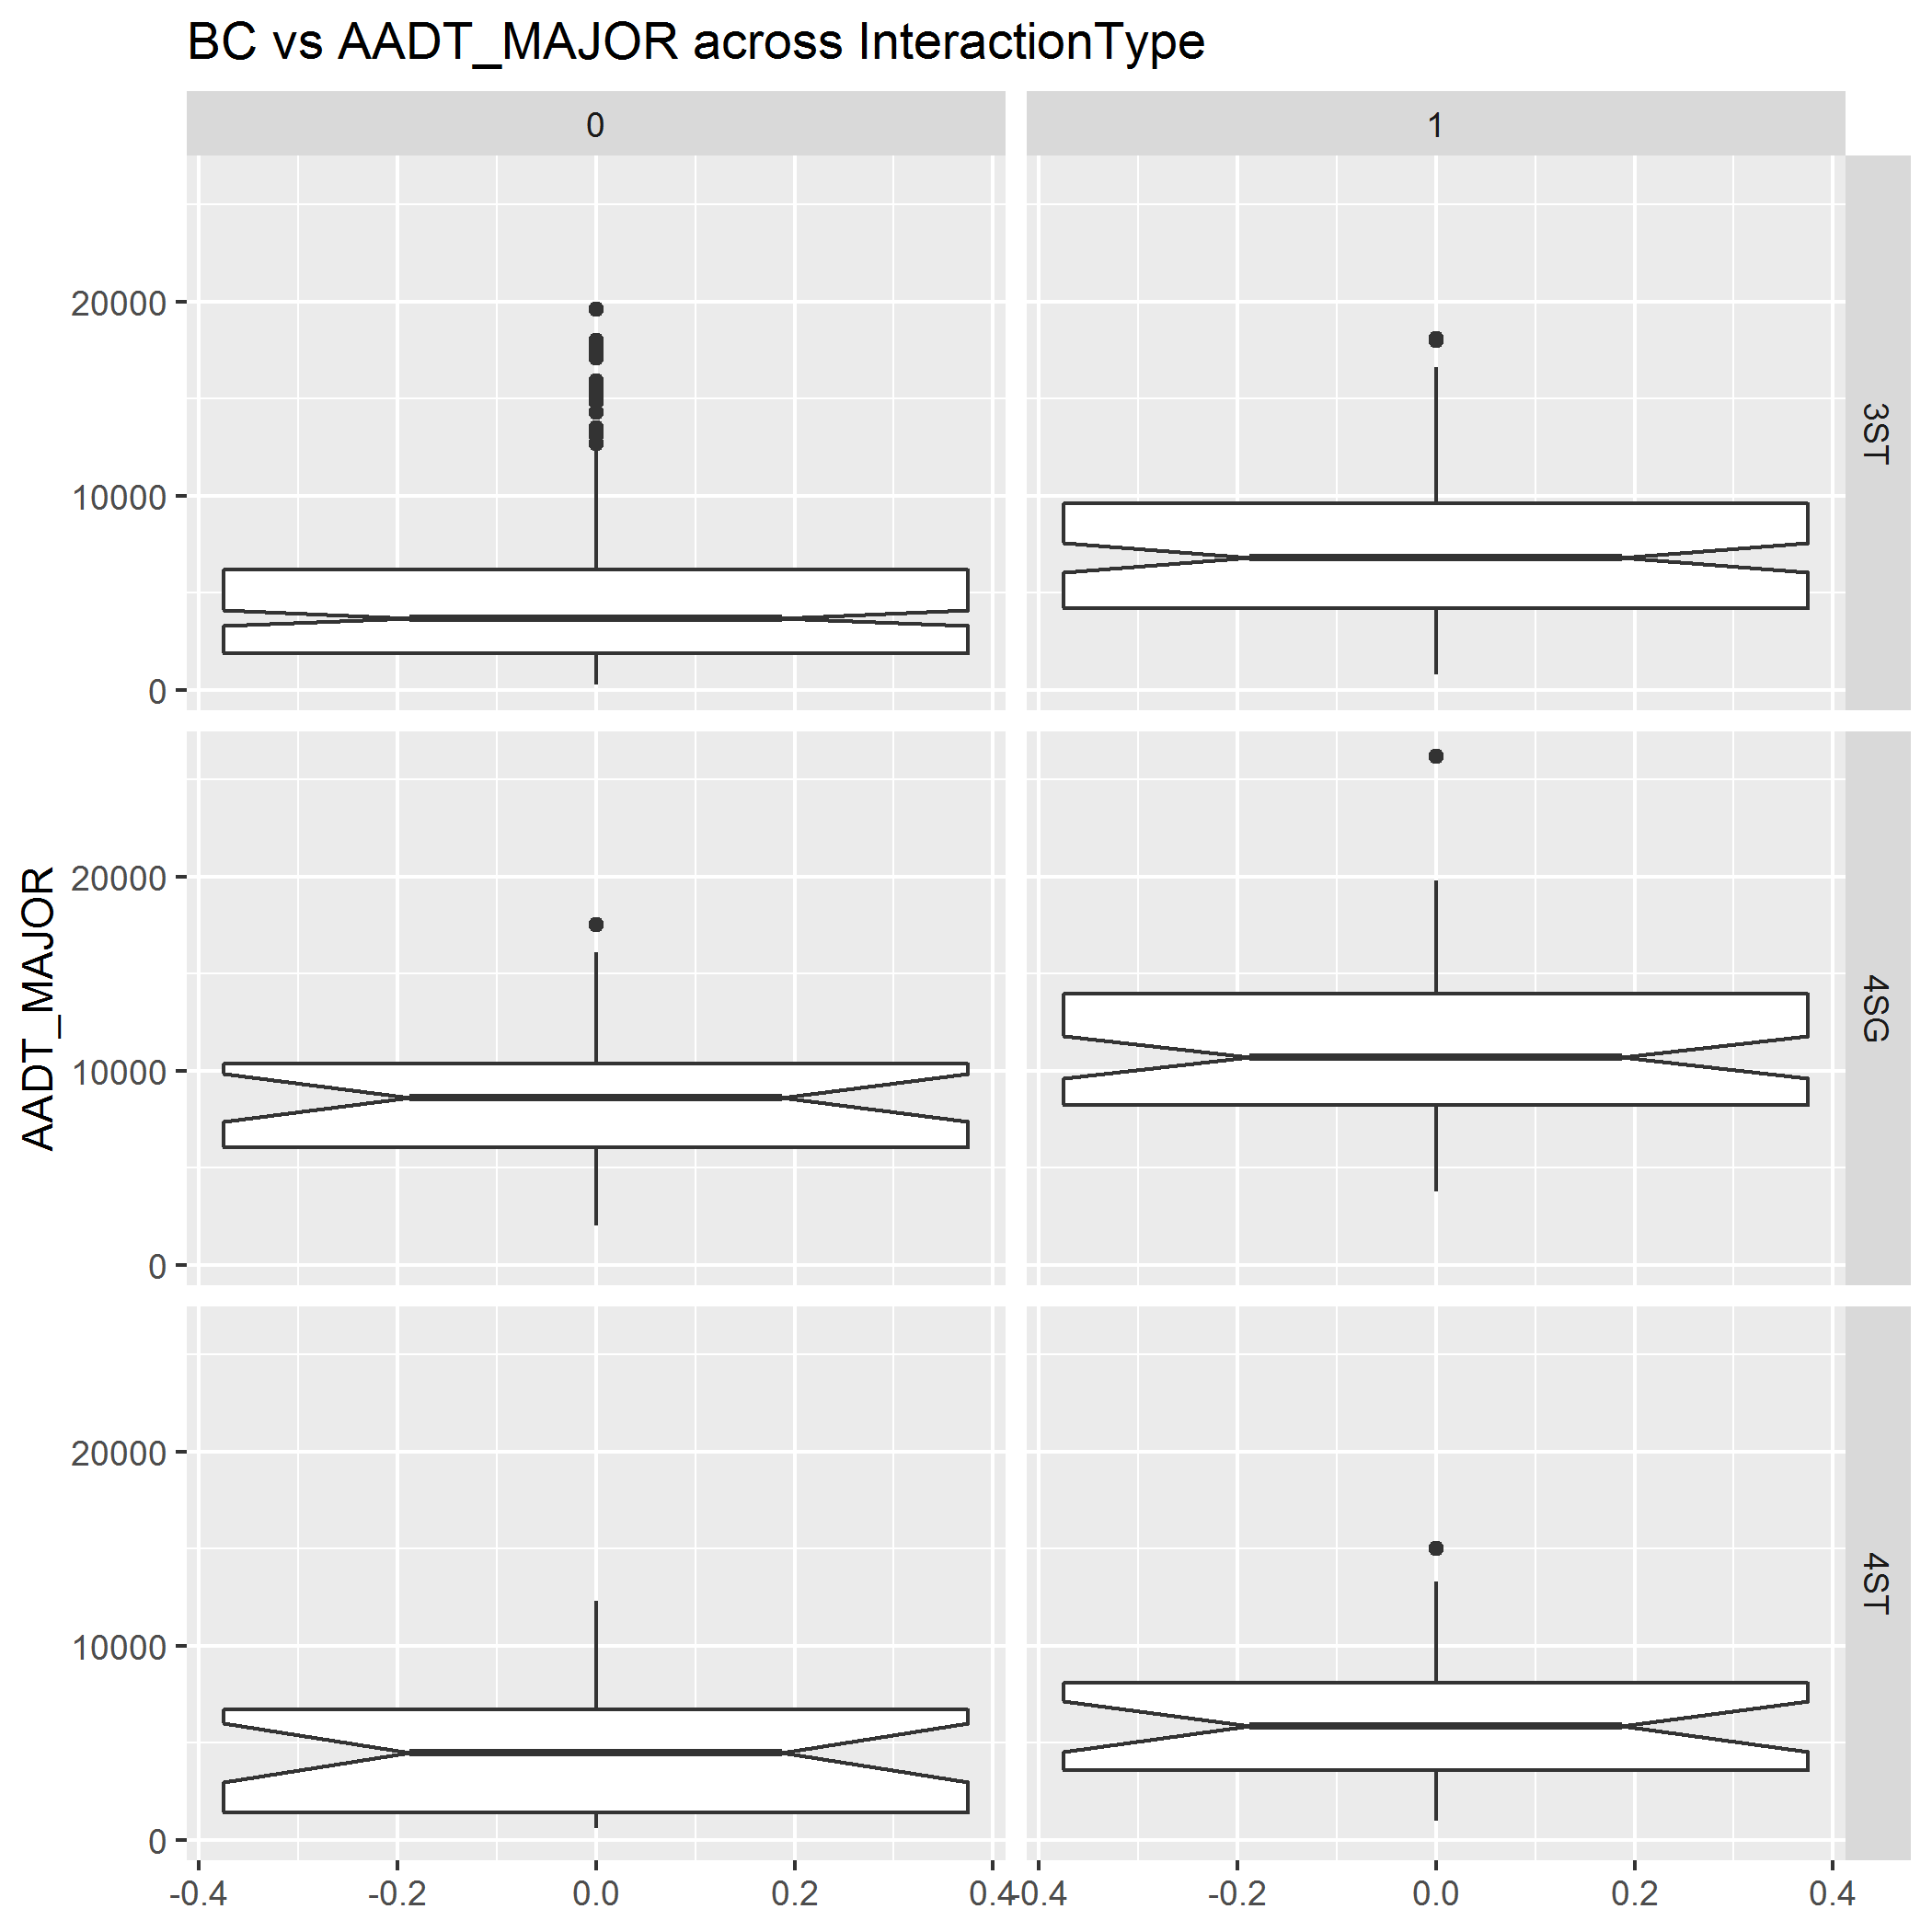
\includegraphics[width=3in]{image/extra4.png}
\small
\end{minipage}
\caption{Extra plots for AADT-Major}
\end{figure}

Extra support plots for AADT-Minor:

\begin{figure}[H]
\begin{minipage}[t]{0.5\linewidth}
\centering
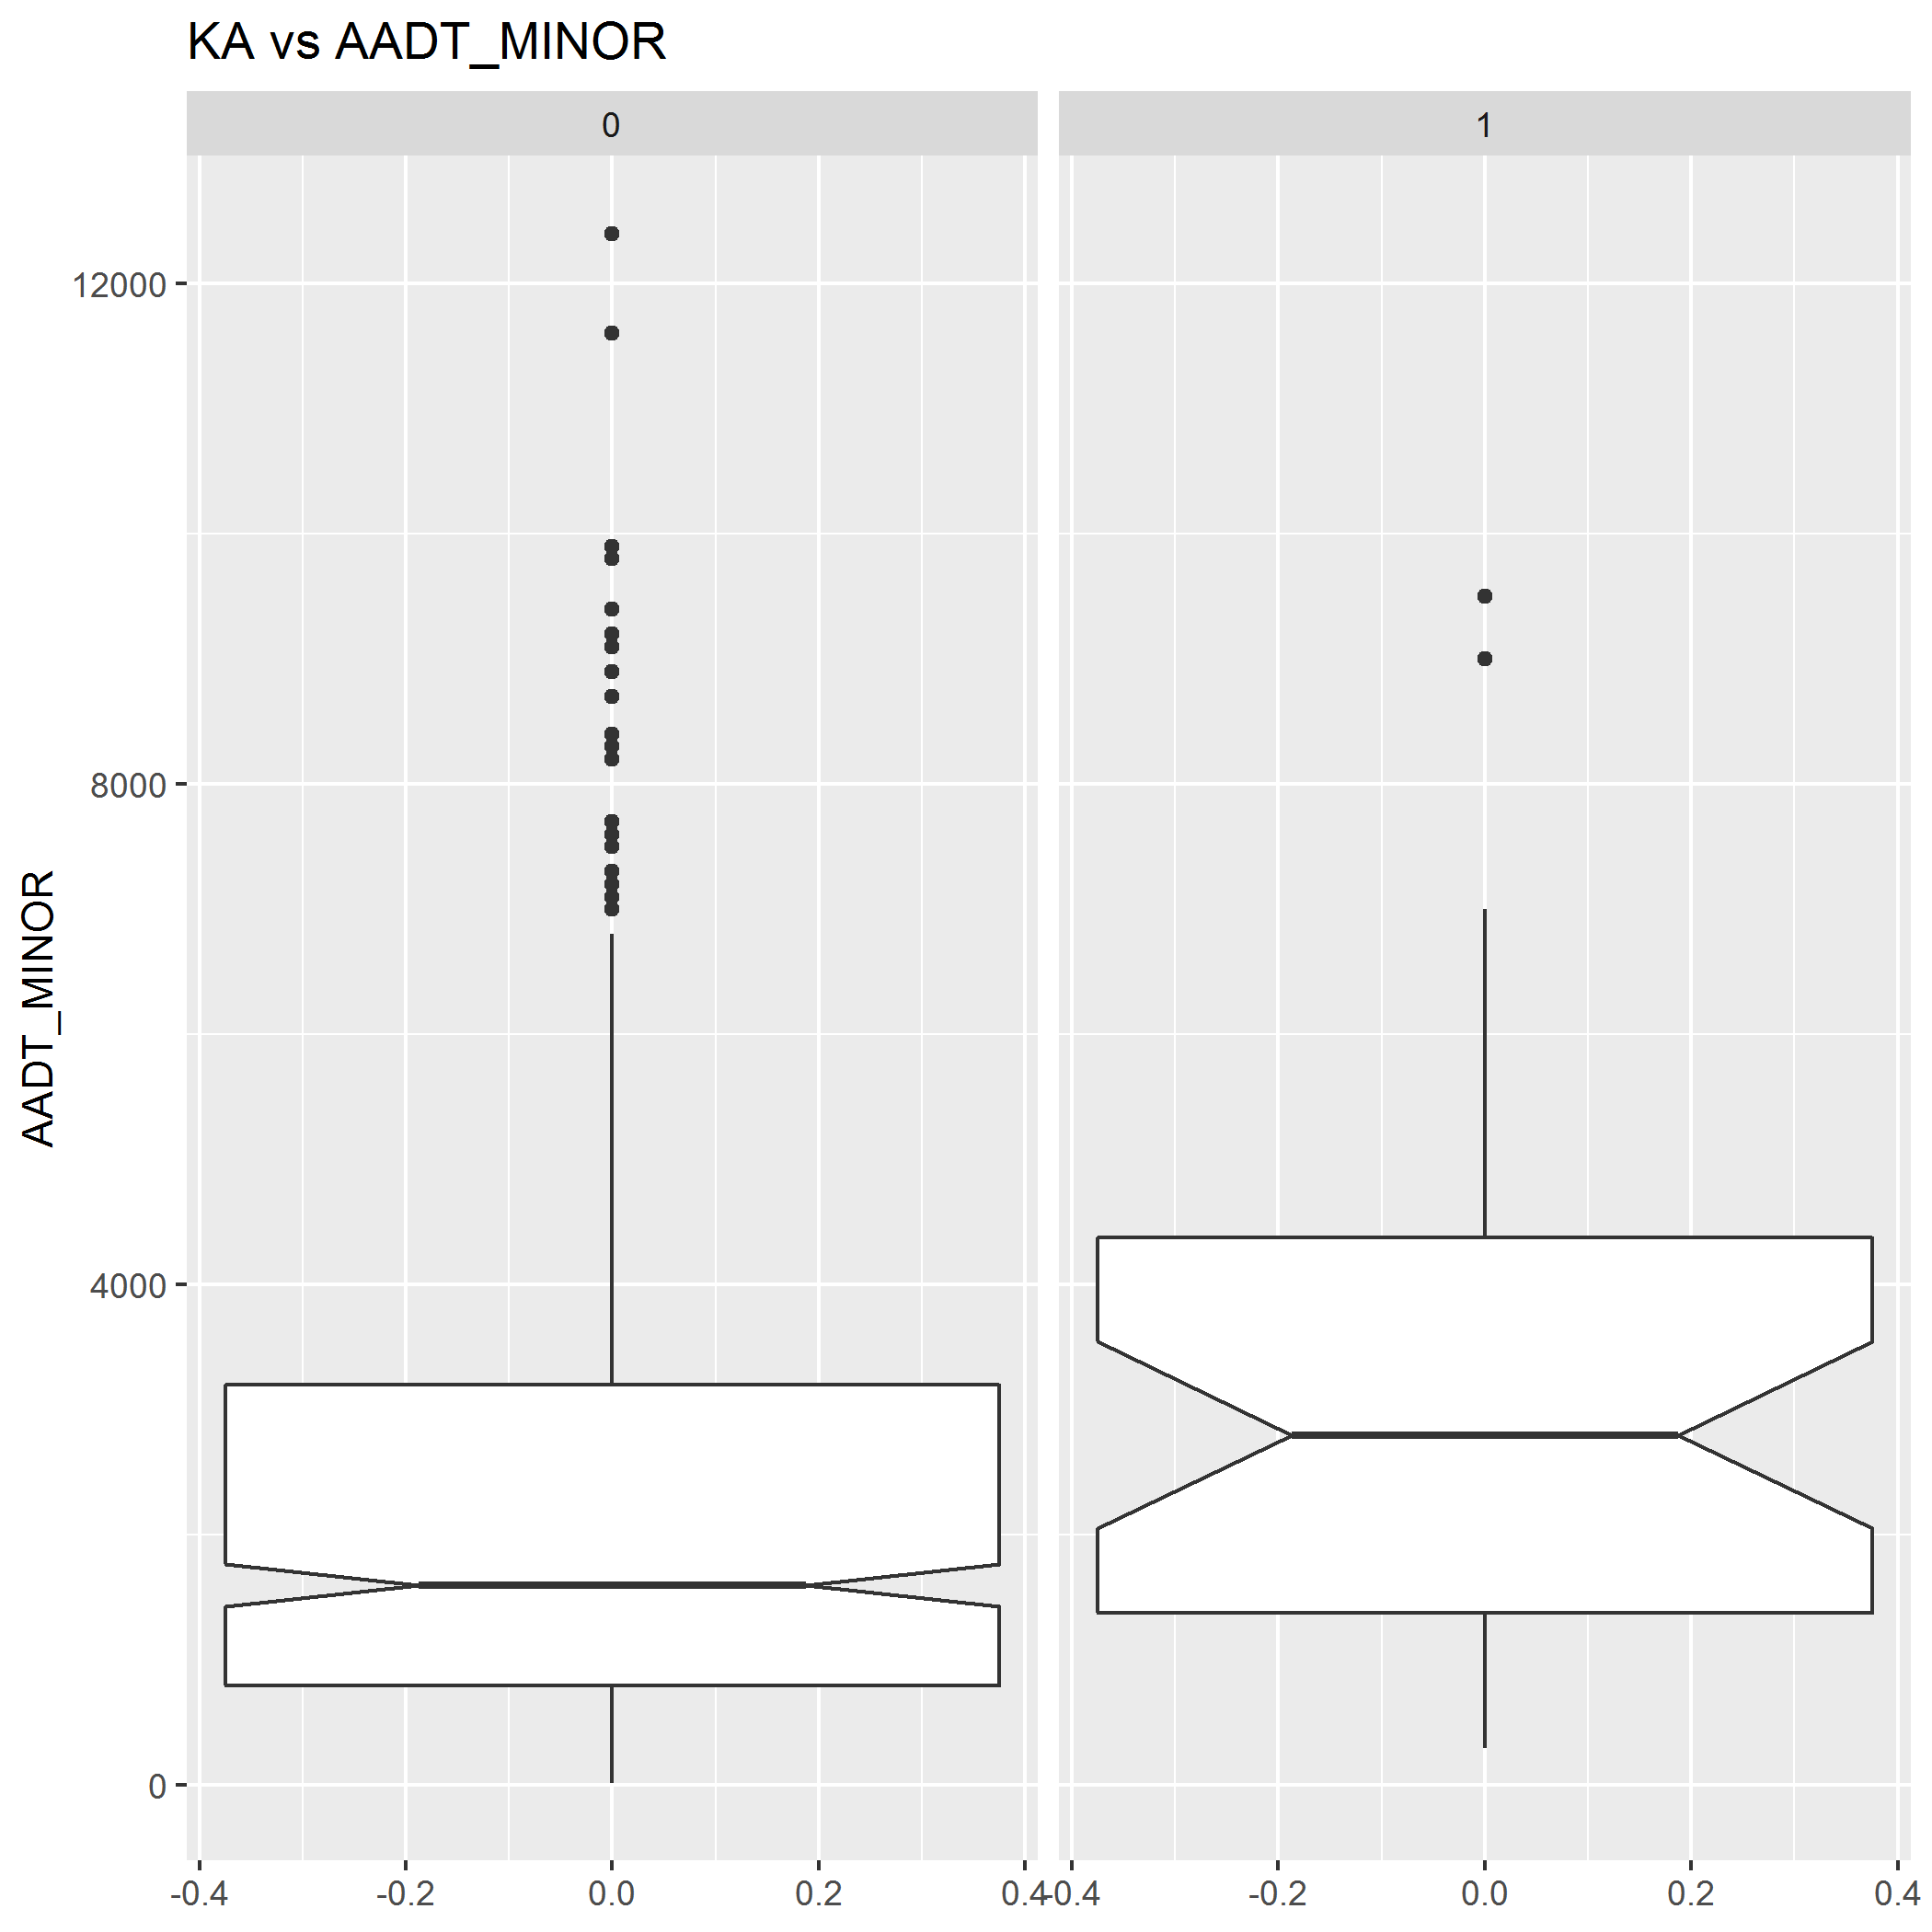
\includegraphics[width=3in]{image/extra5.png}
\small
\end{minipage}
\begin{minipage}[t]{0.5\linewidth}
\centering
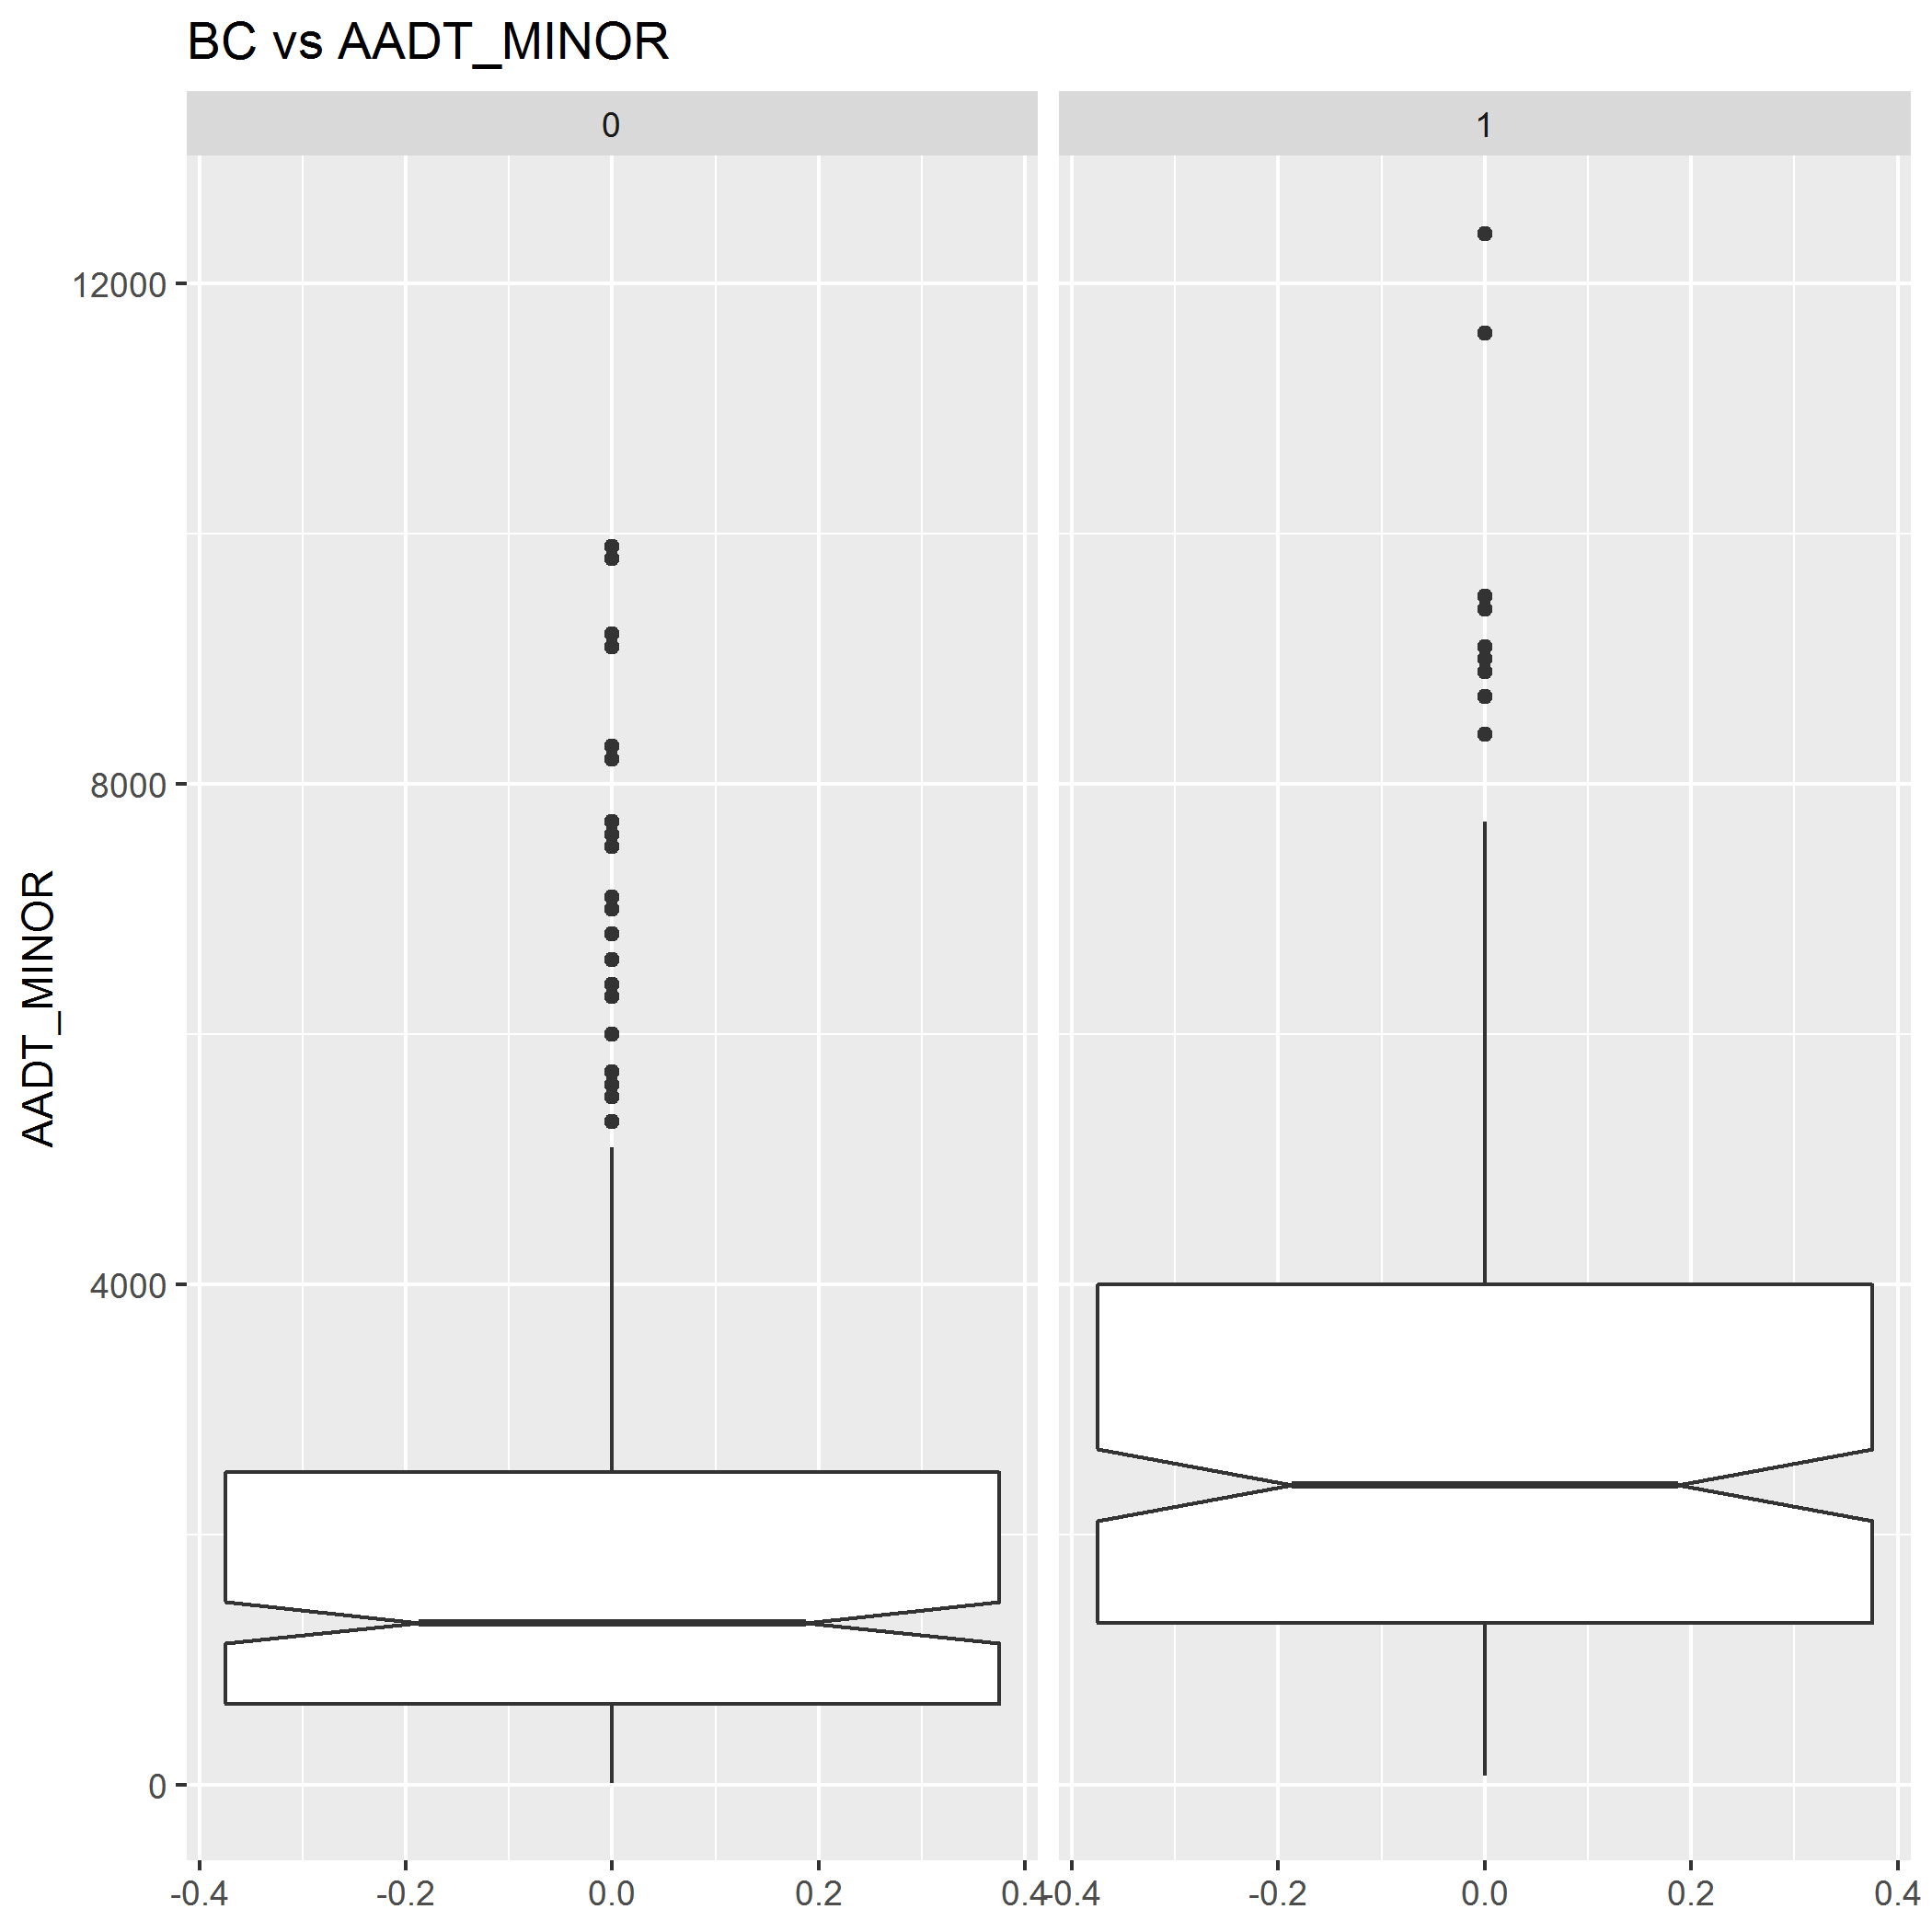
\includegraphics[width=3in]{image/extra6.png}
\small
\end{minipage}
\begin{minipage}[t]{0.5\linewidth}
\centering
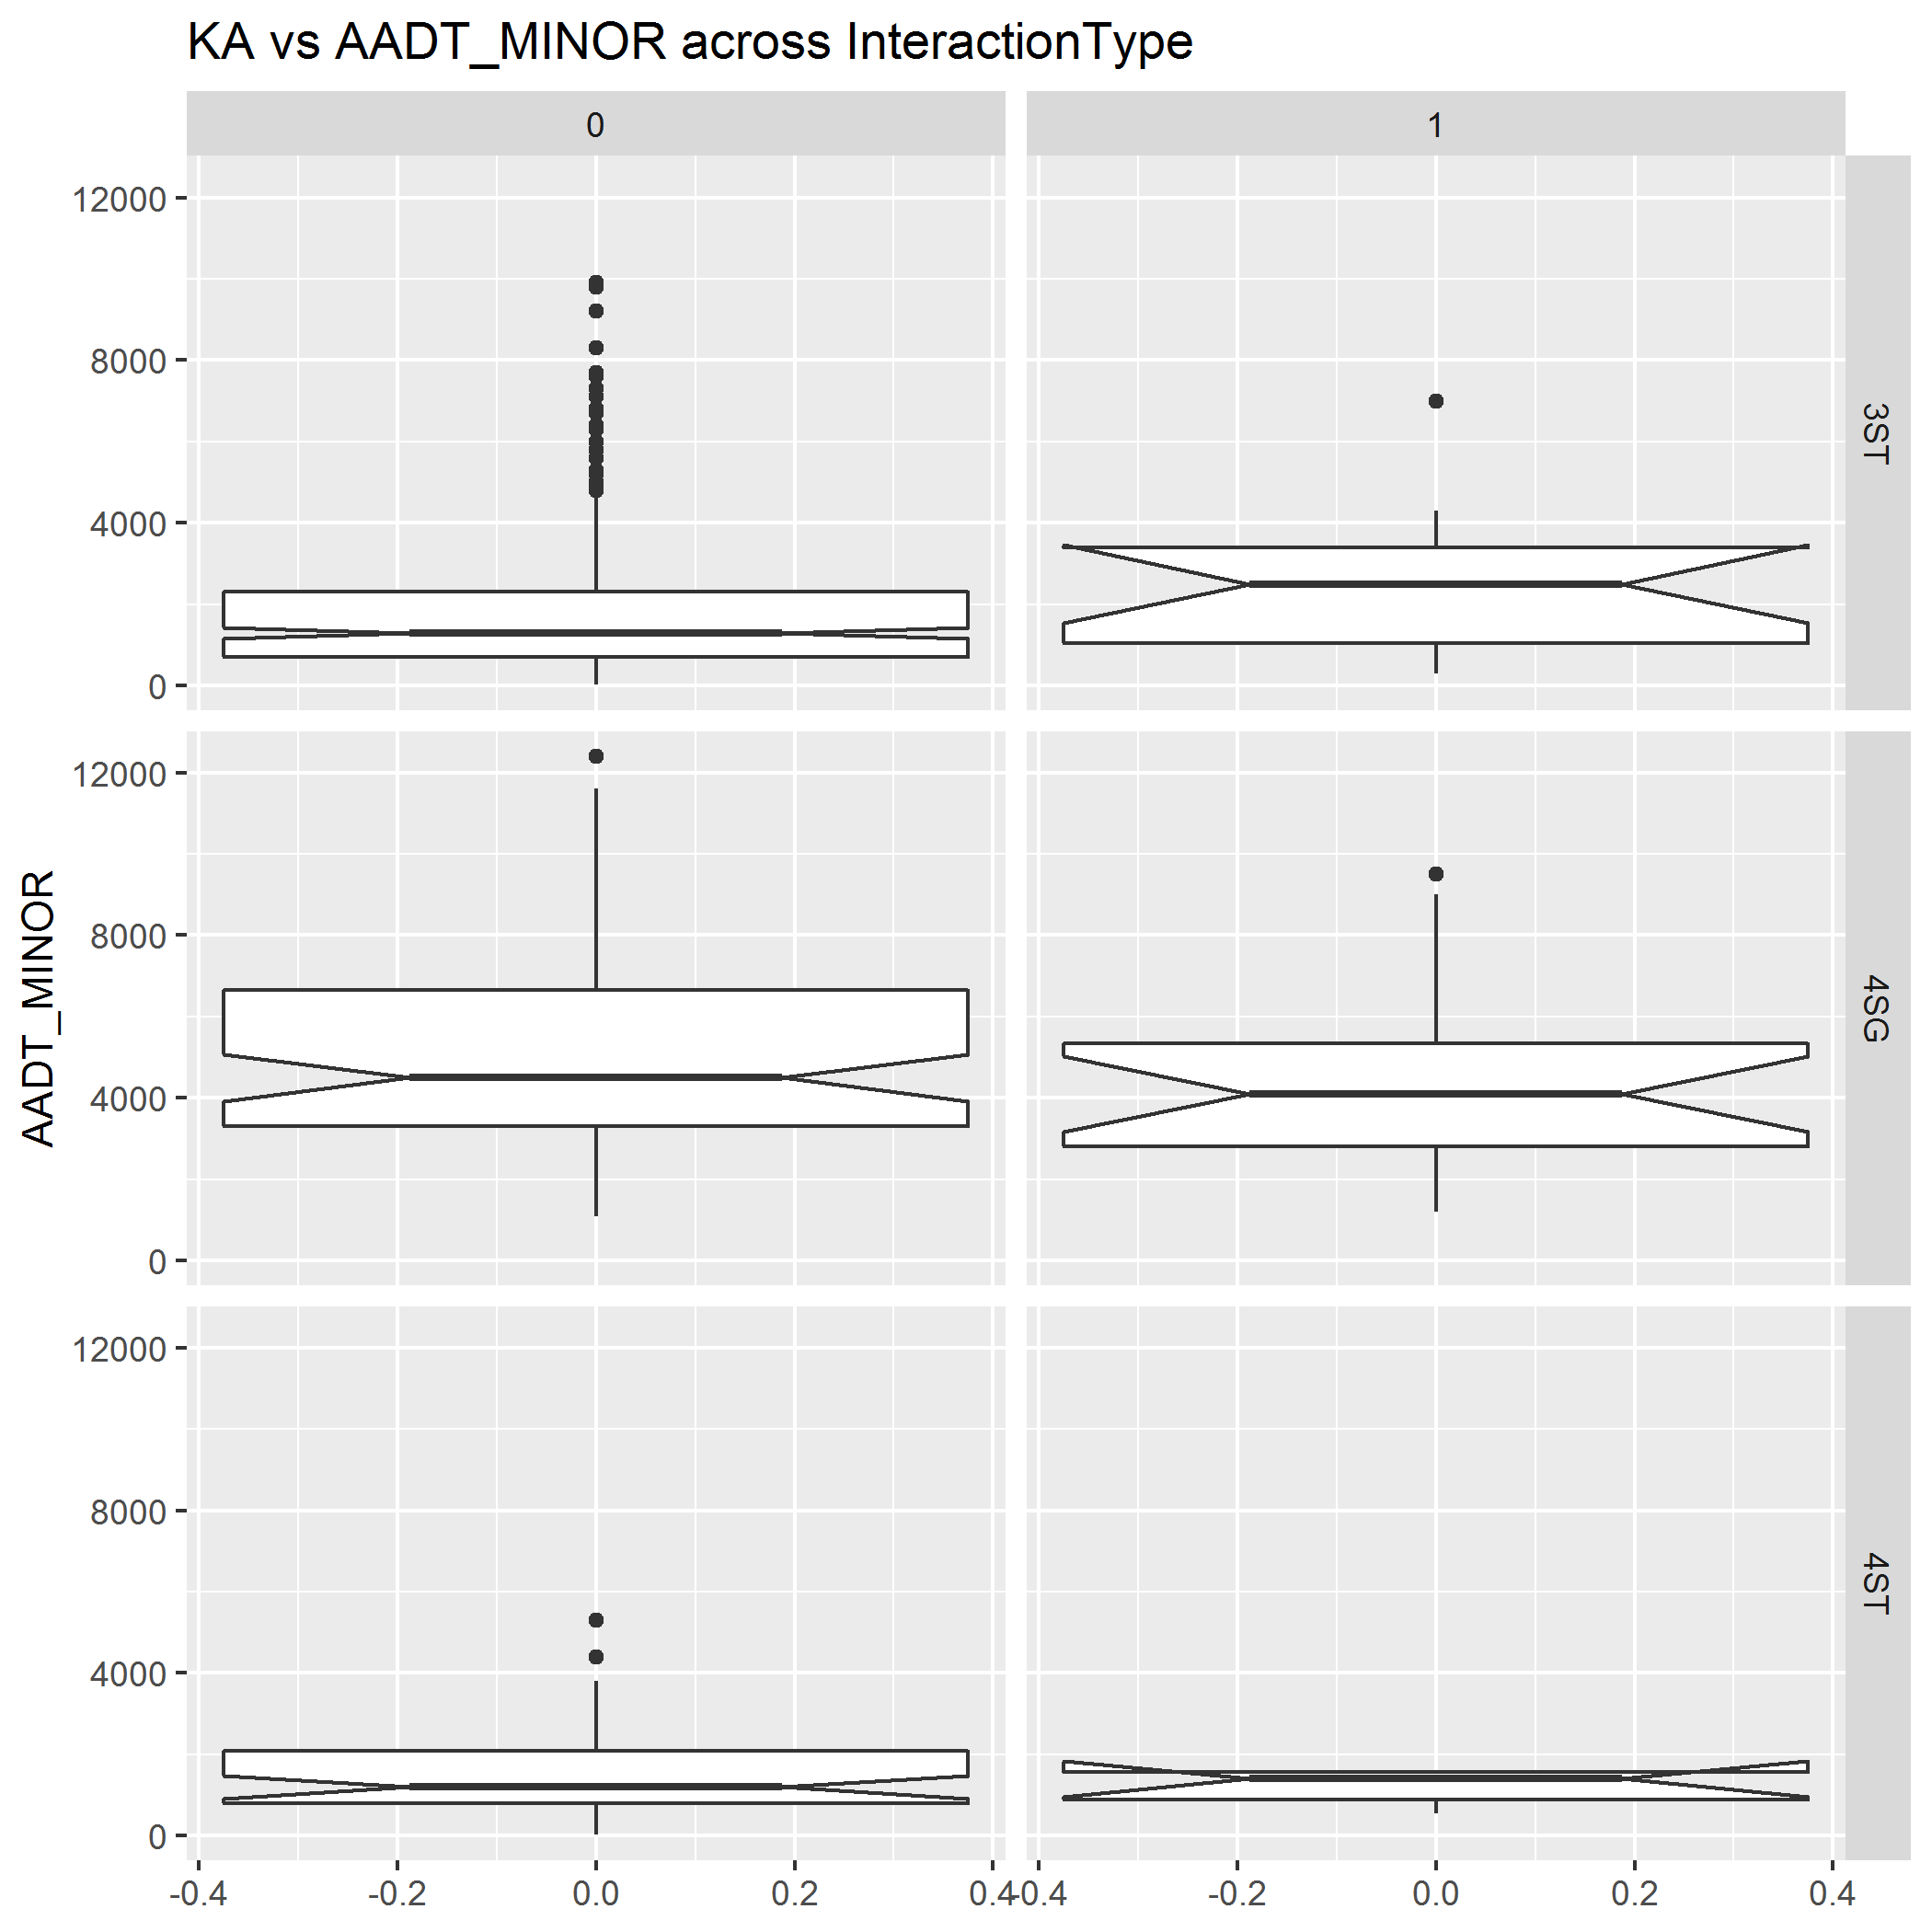
\includegraphics[width=3in]{image/extra7.png}
\small
\end{minipage}
\begin{minipage}[t]{0.5\linewidth}
\centering
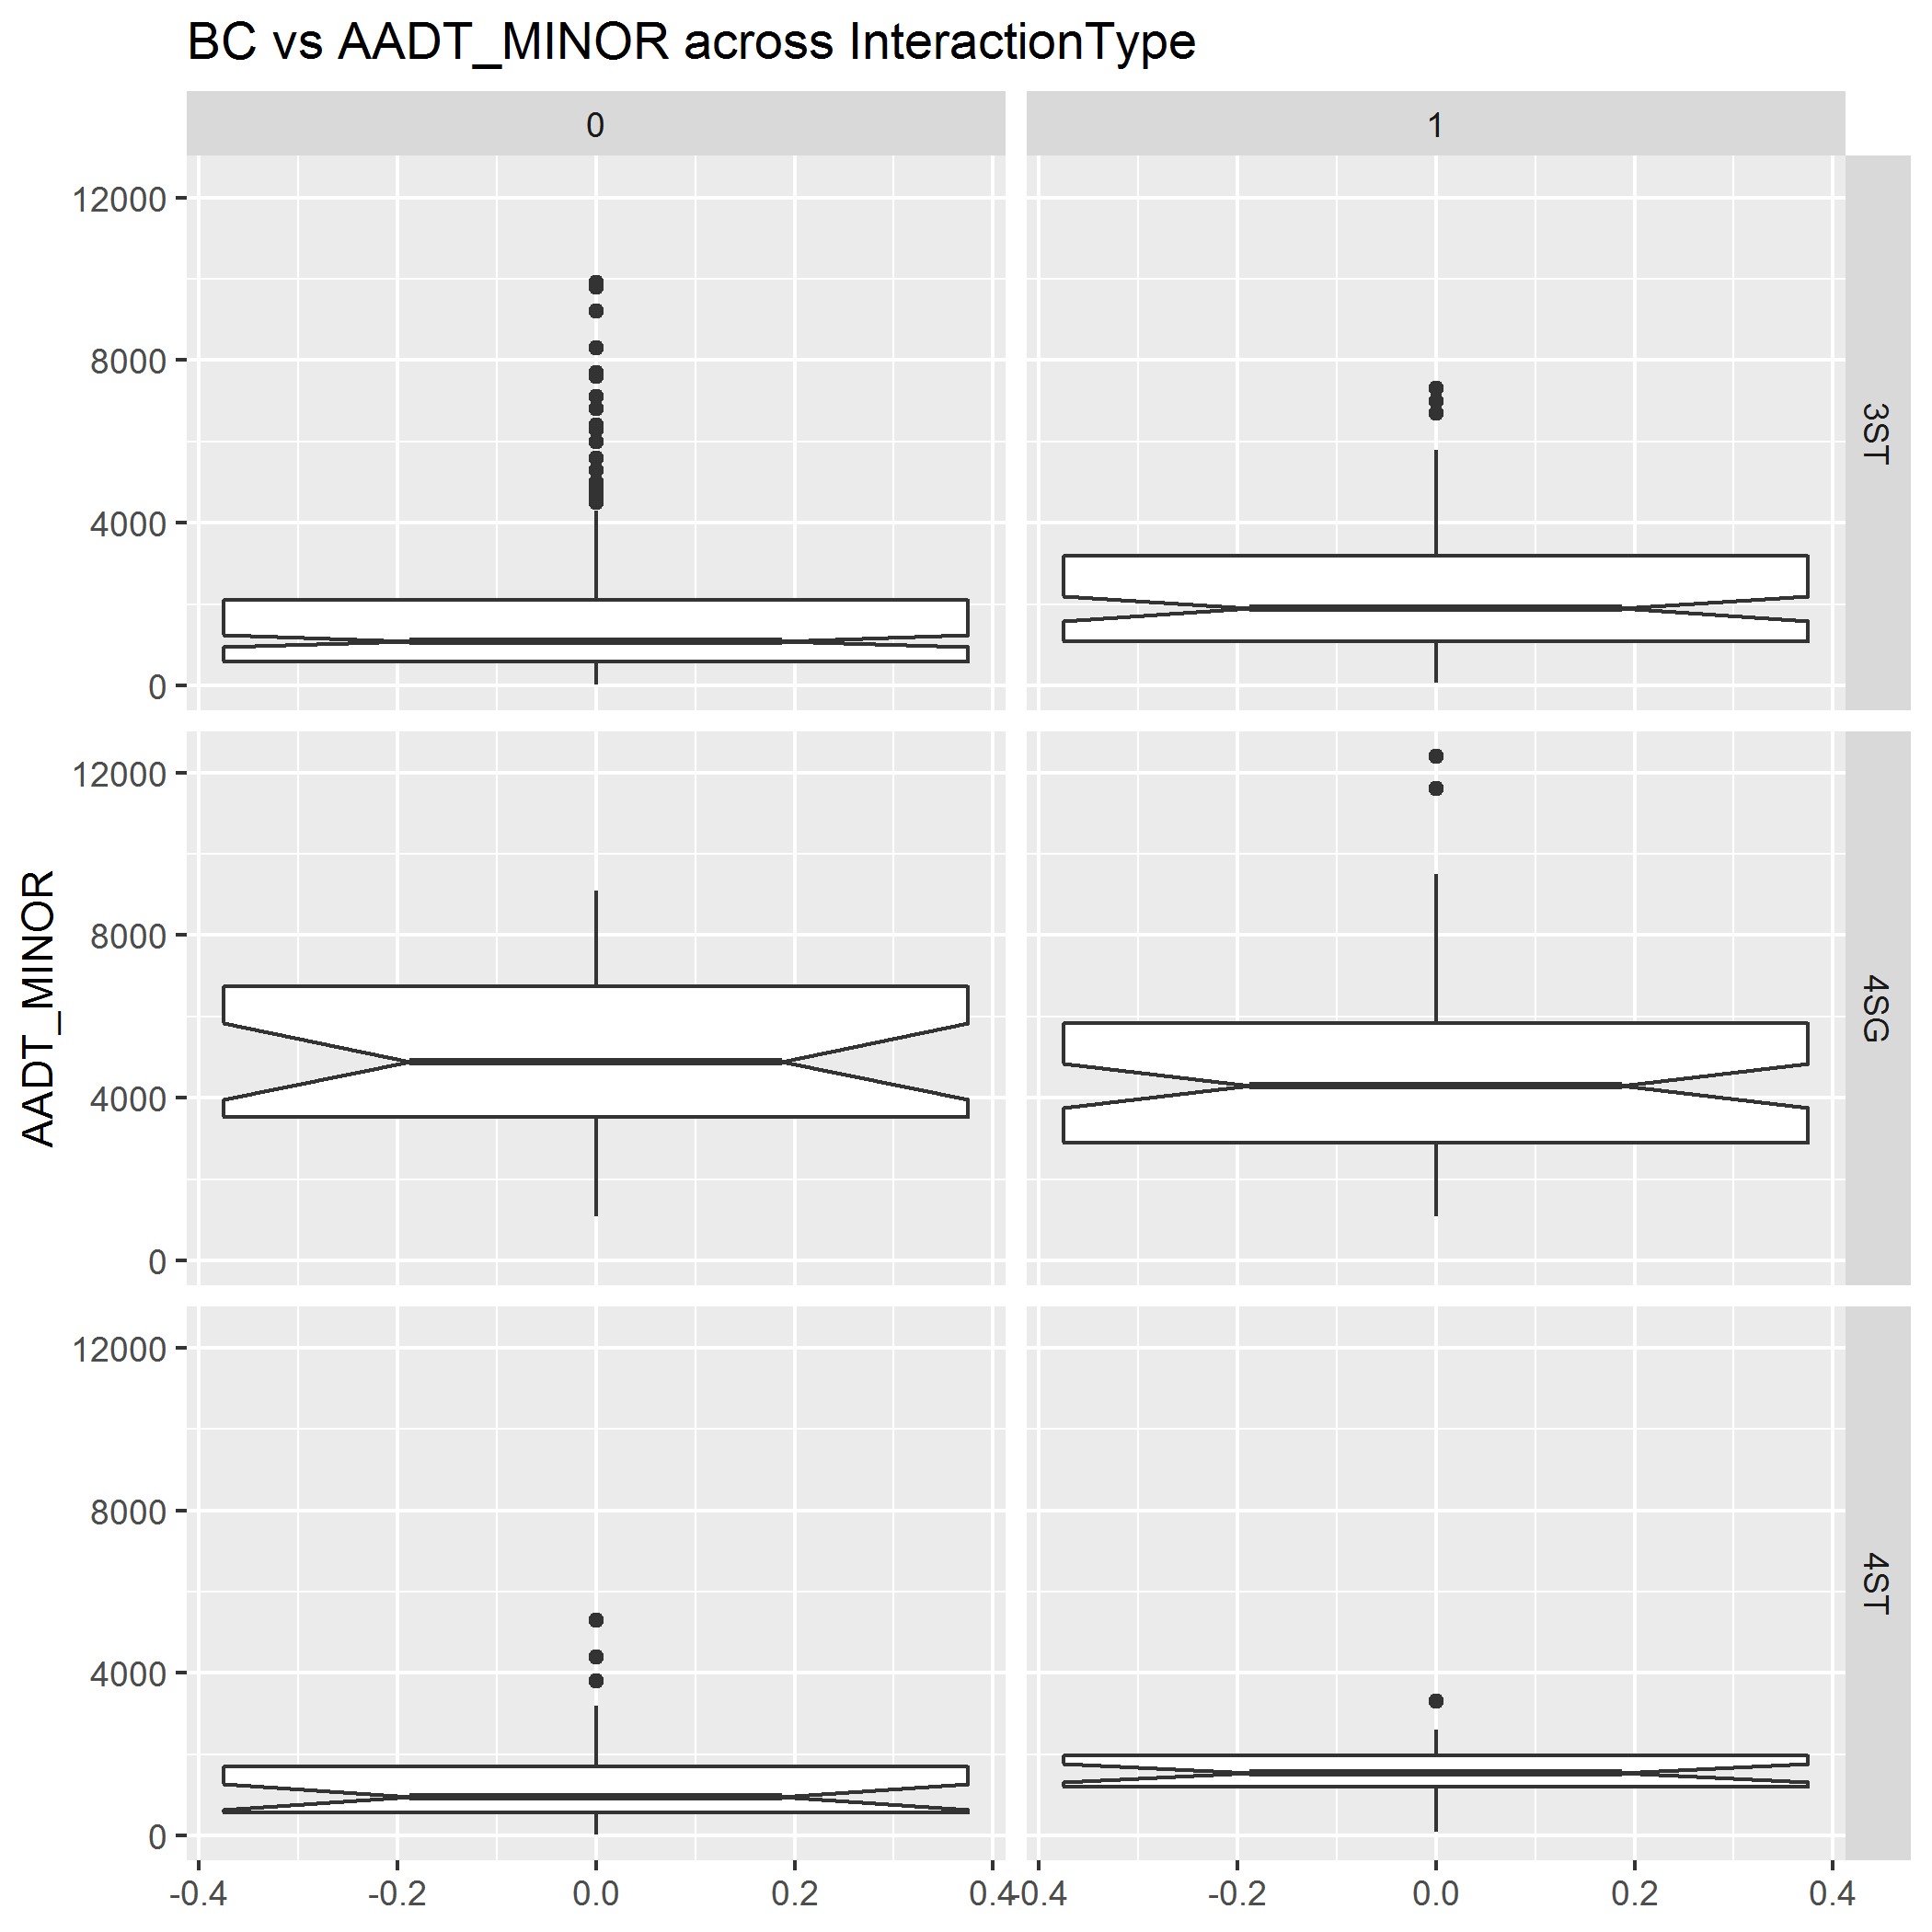
\includegraphics[width=3in]{image/extra8.png}
\small
\end{minipage}
\caption{Extra plots for AADT-Minor}
\end{figure}

Extra support plots for Skew Angle:

\begin{figure}[H]
\begin{minipage}[t]{0.5\linewidth}
\centering
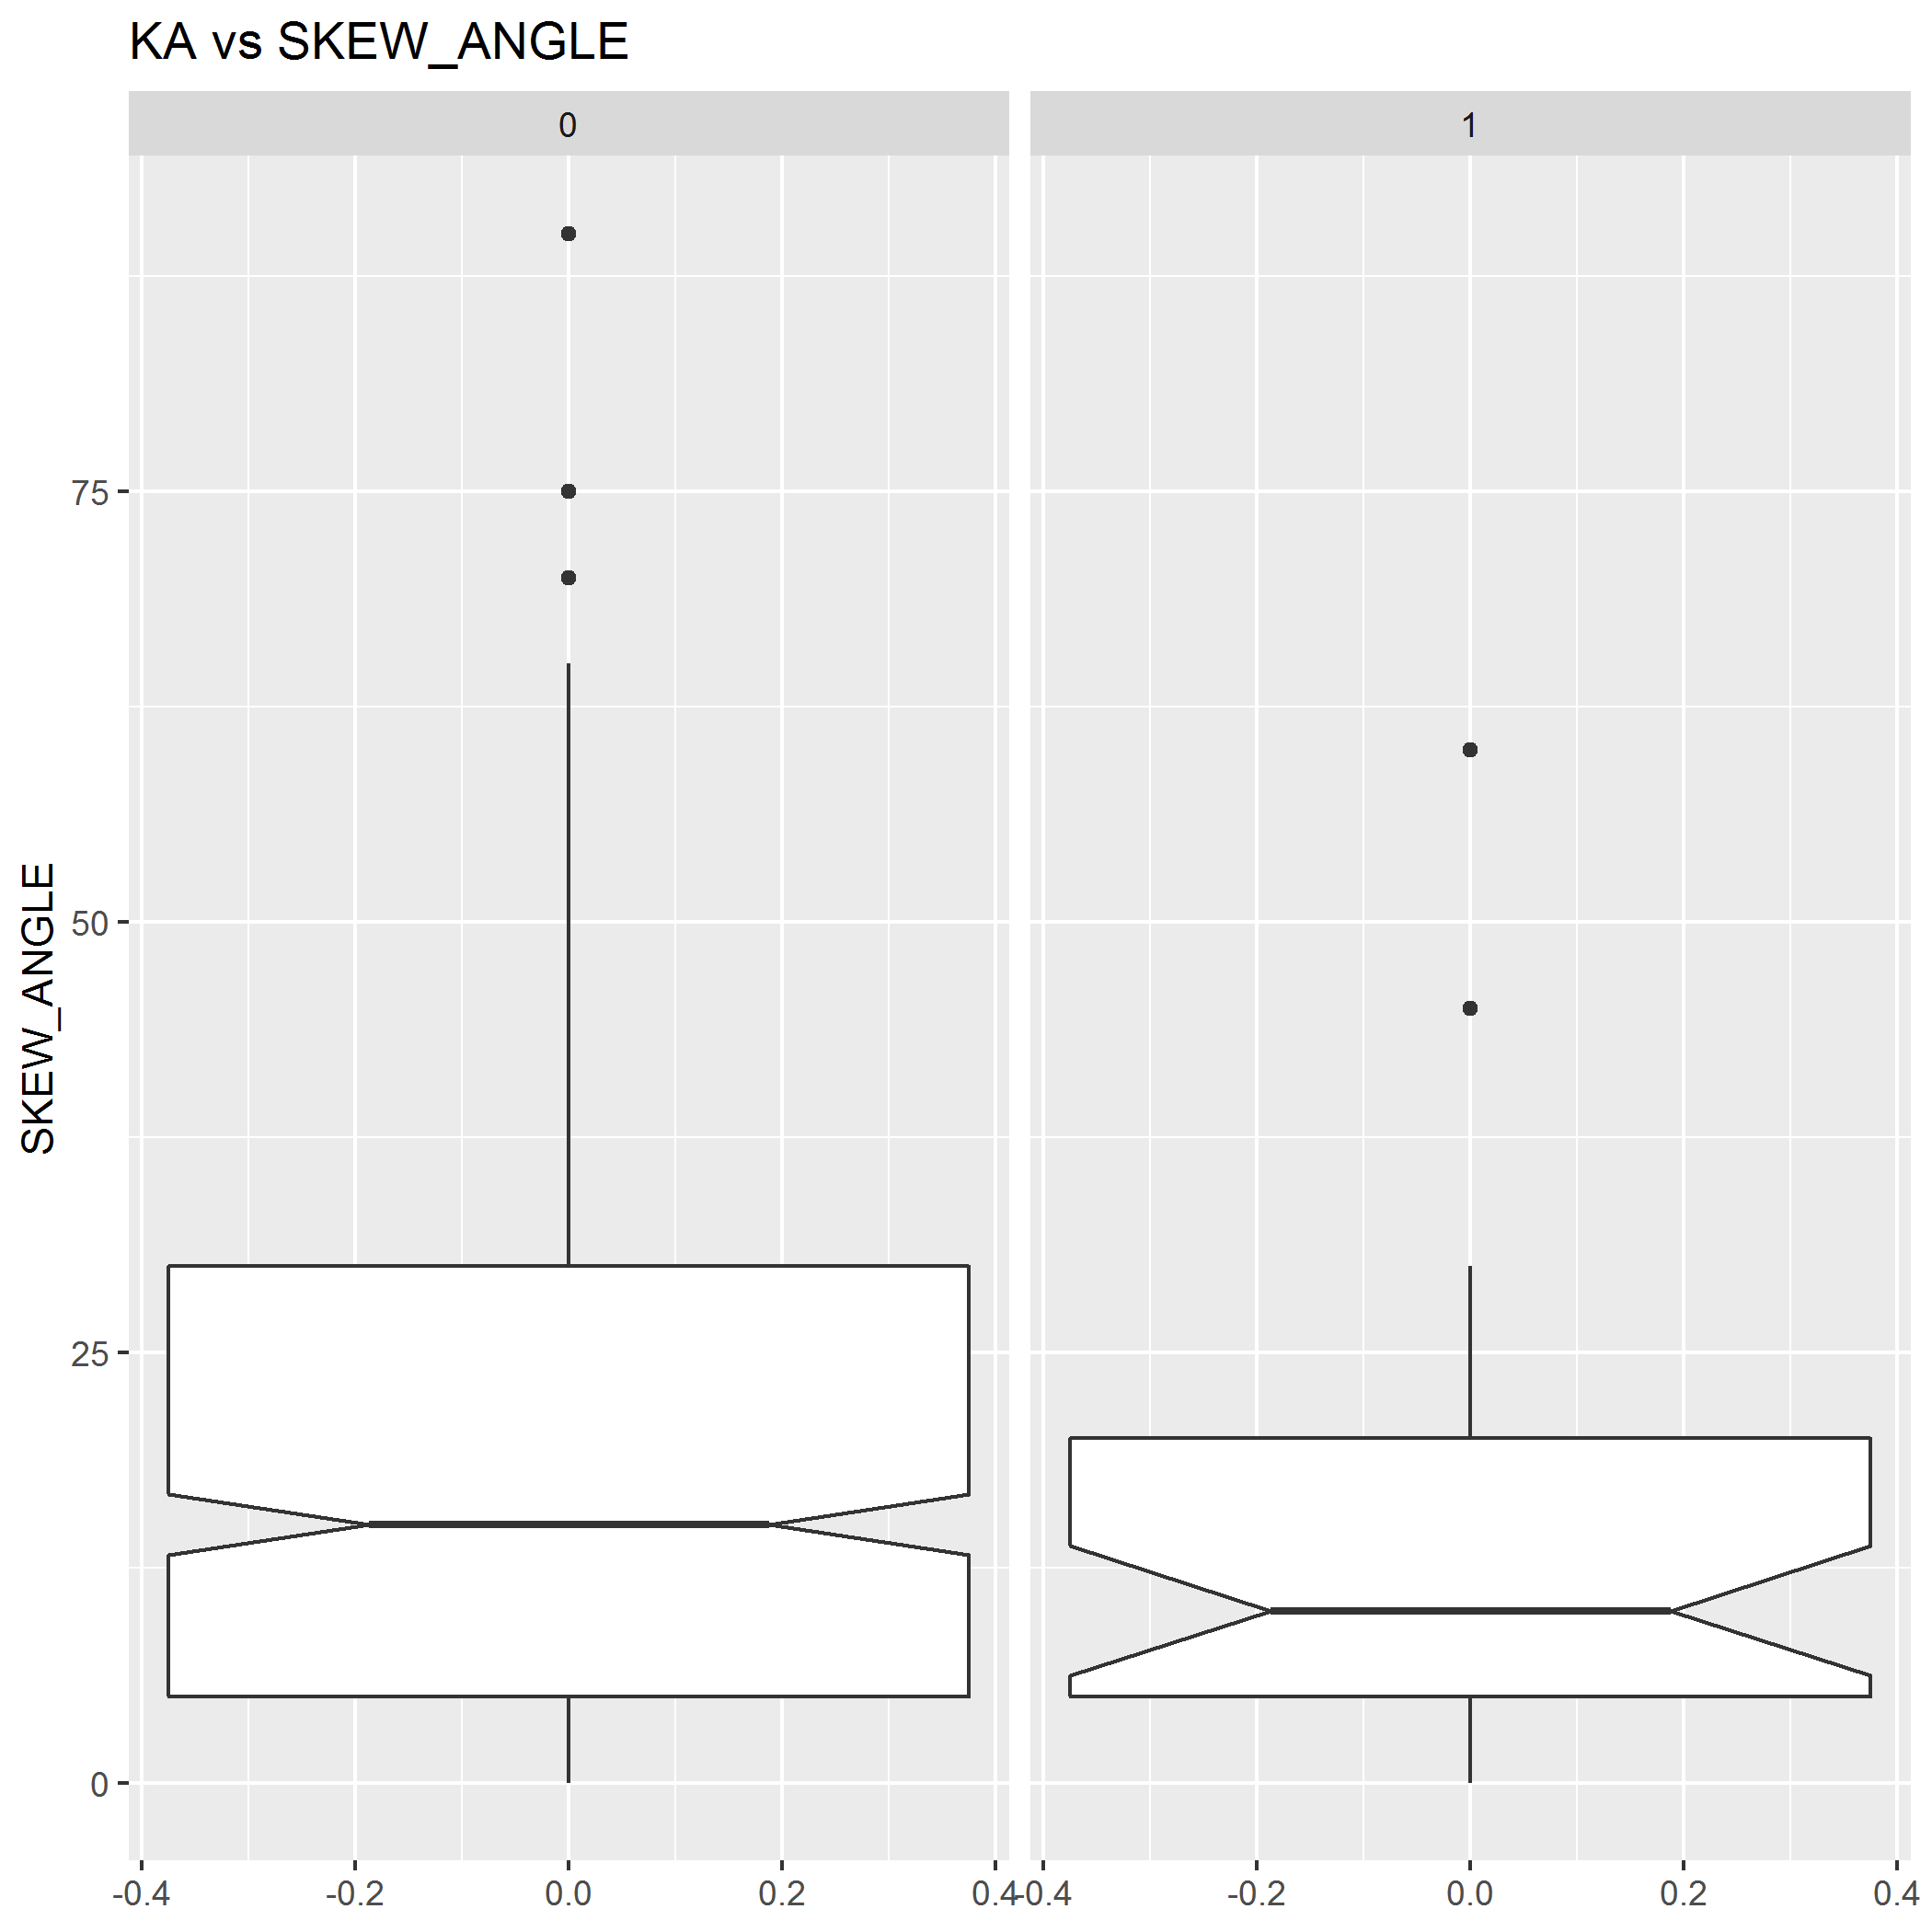
\includegraphics[width=3in]{image/extra9.png}
\small
\end{minipage}
\begin{minipage}[t]{0.5\linewidth}
\centering
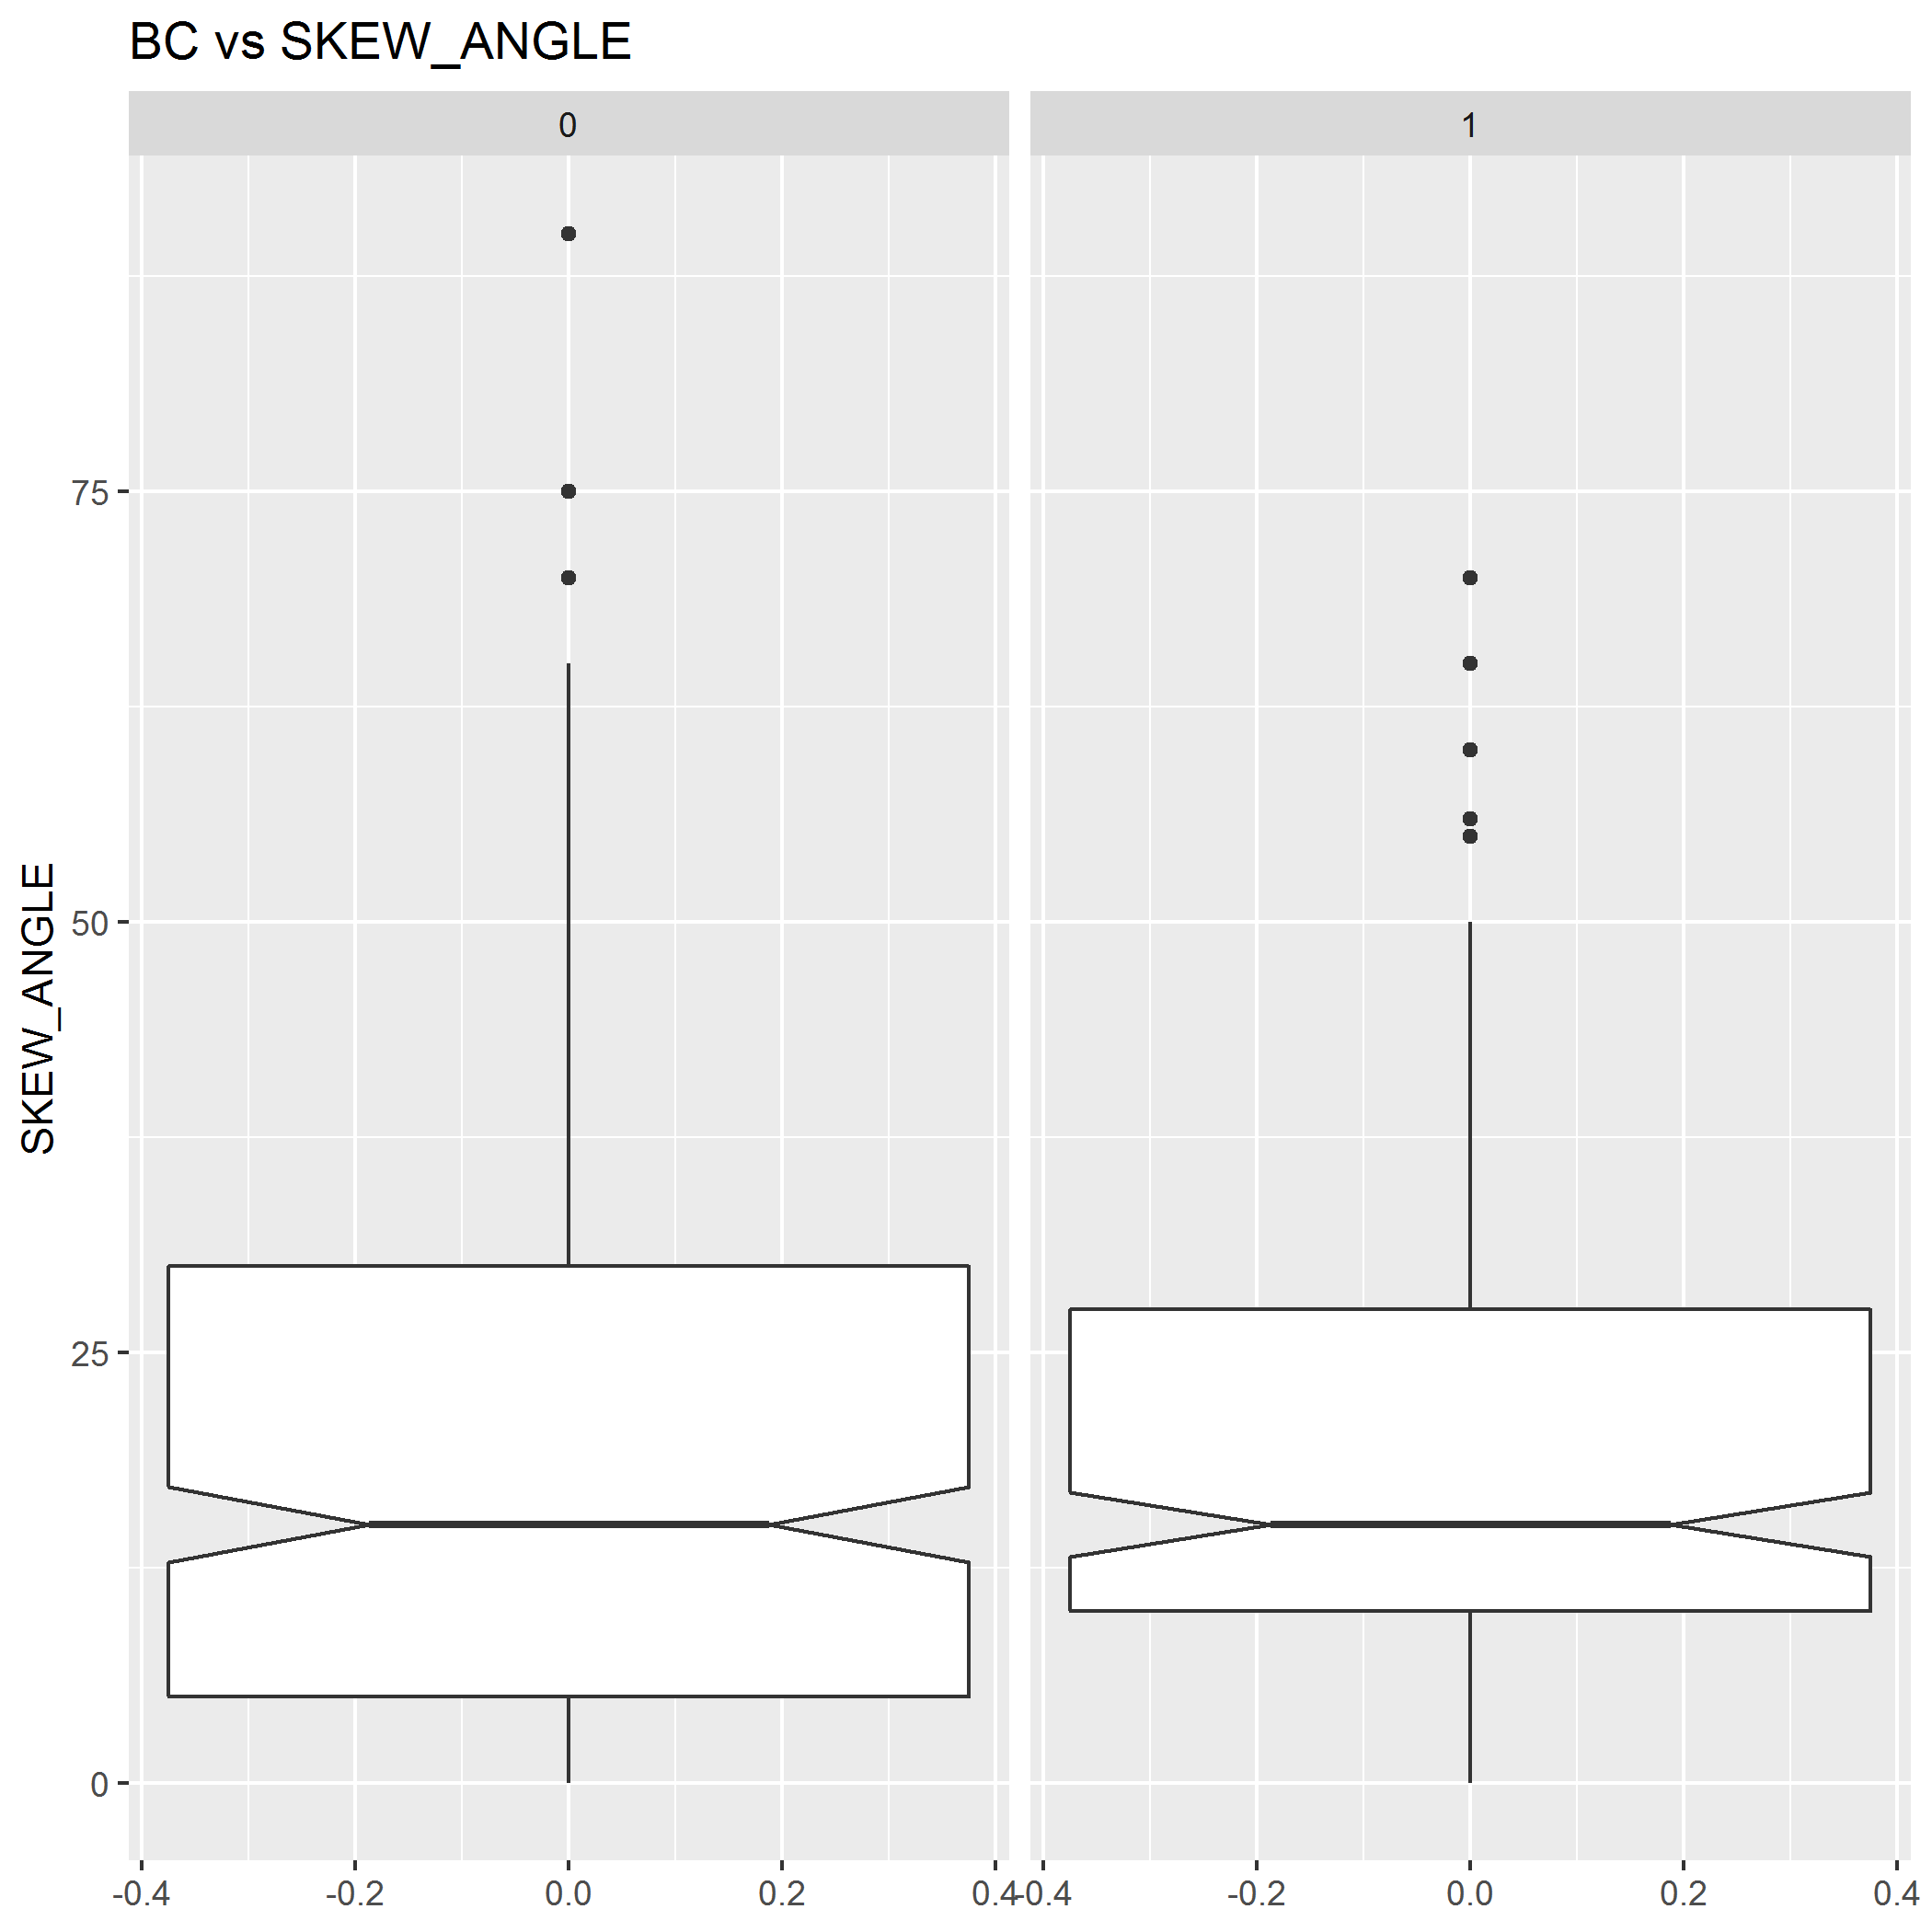
\includegraphics[width=3in]{image/extra10.png}
\small
\end{minipage}
\begin{minipage}[t]{0.5\linewidth}
\centering
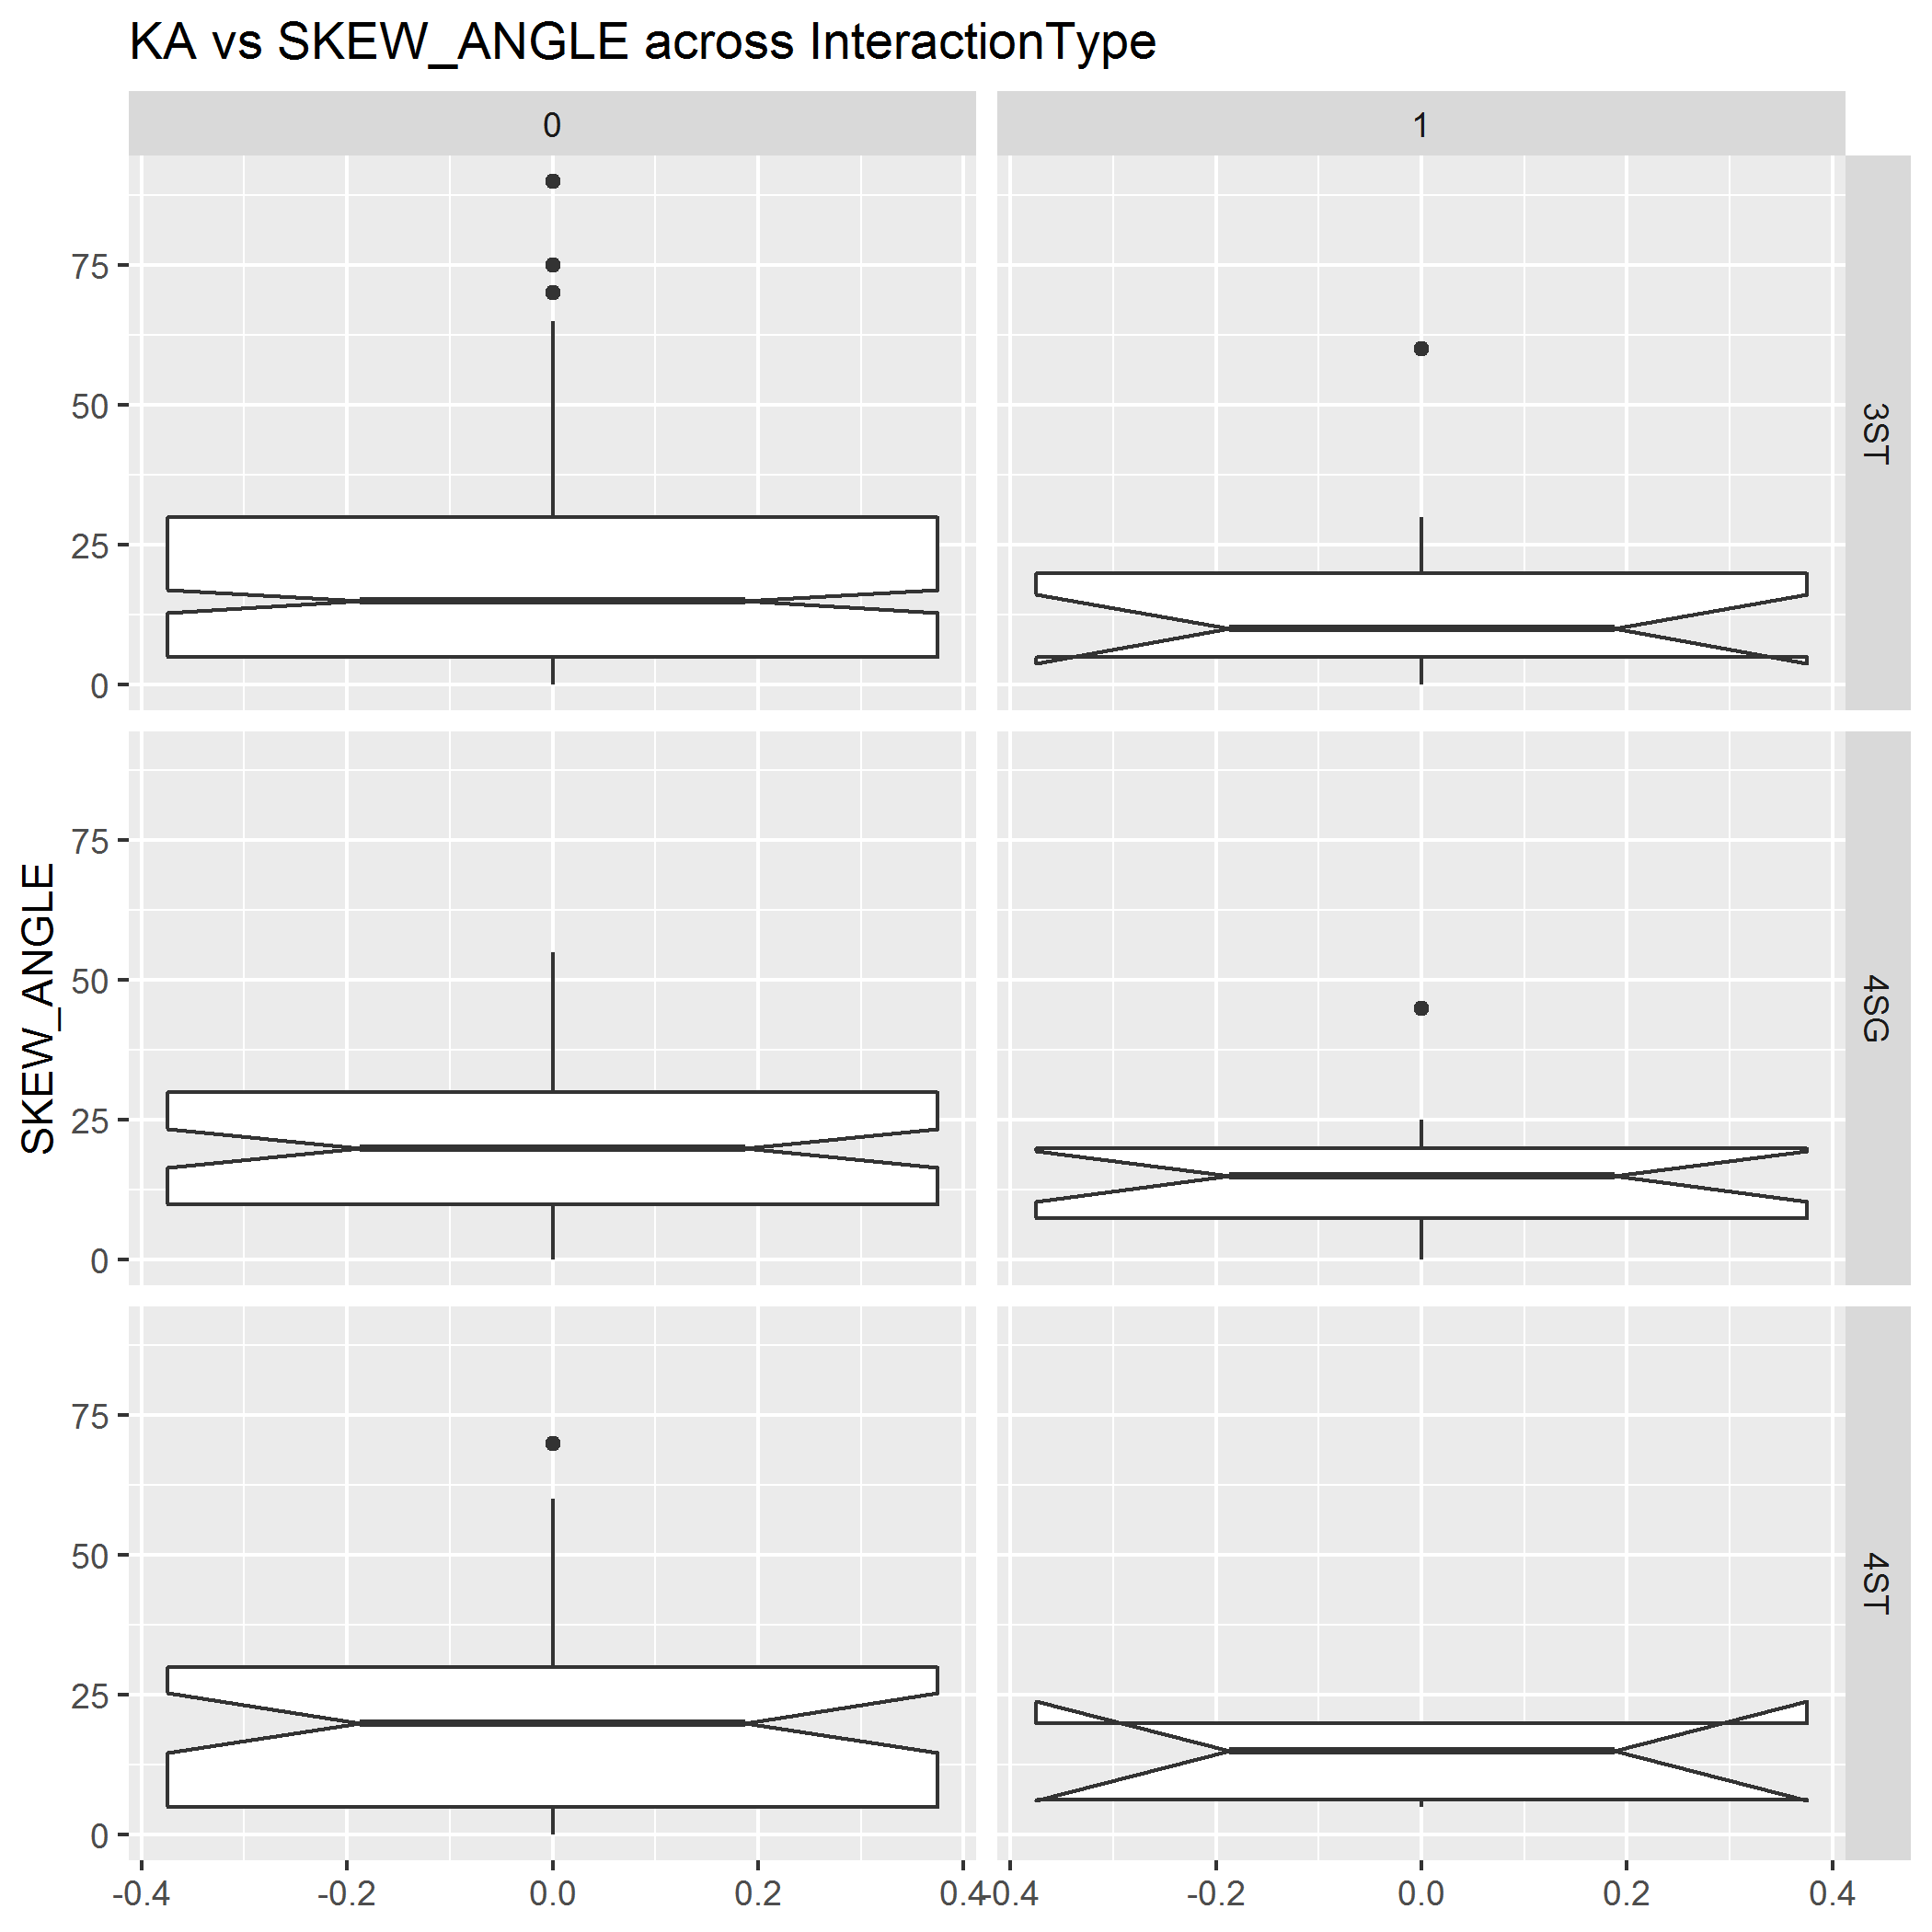
\includegraphics[width=3in]{image/extra11.png}
\small
\end{minipage}
\begin{minipage}[t]{0.5\linewidth}
\centering
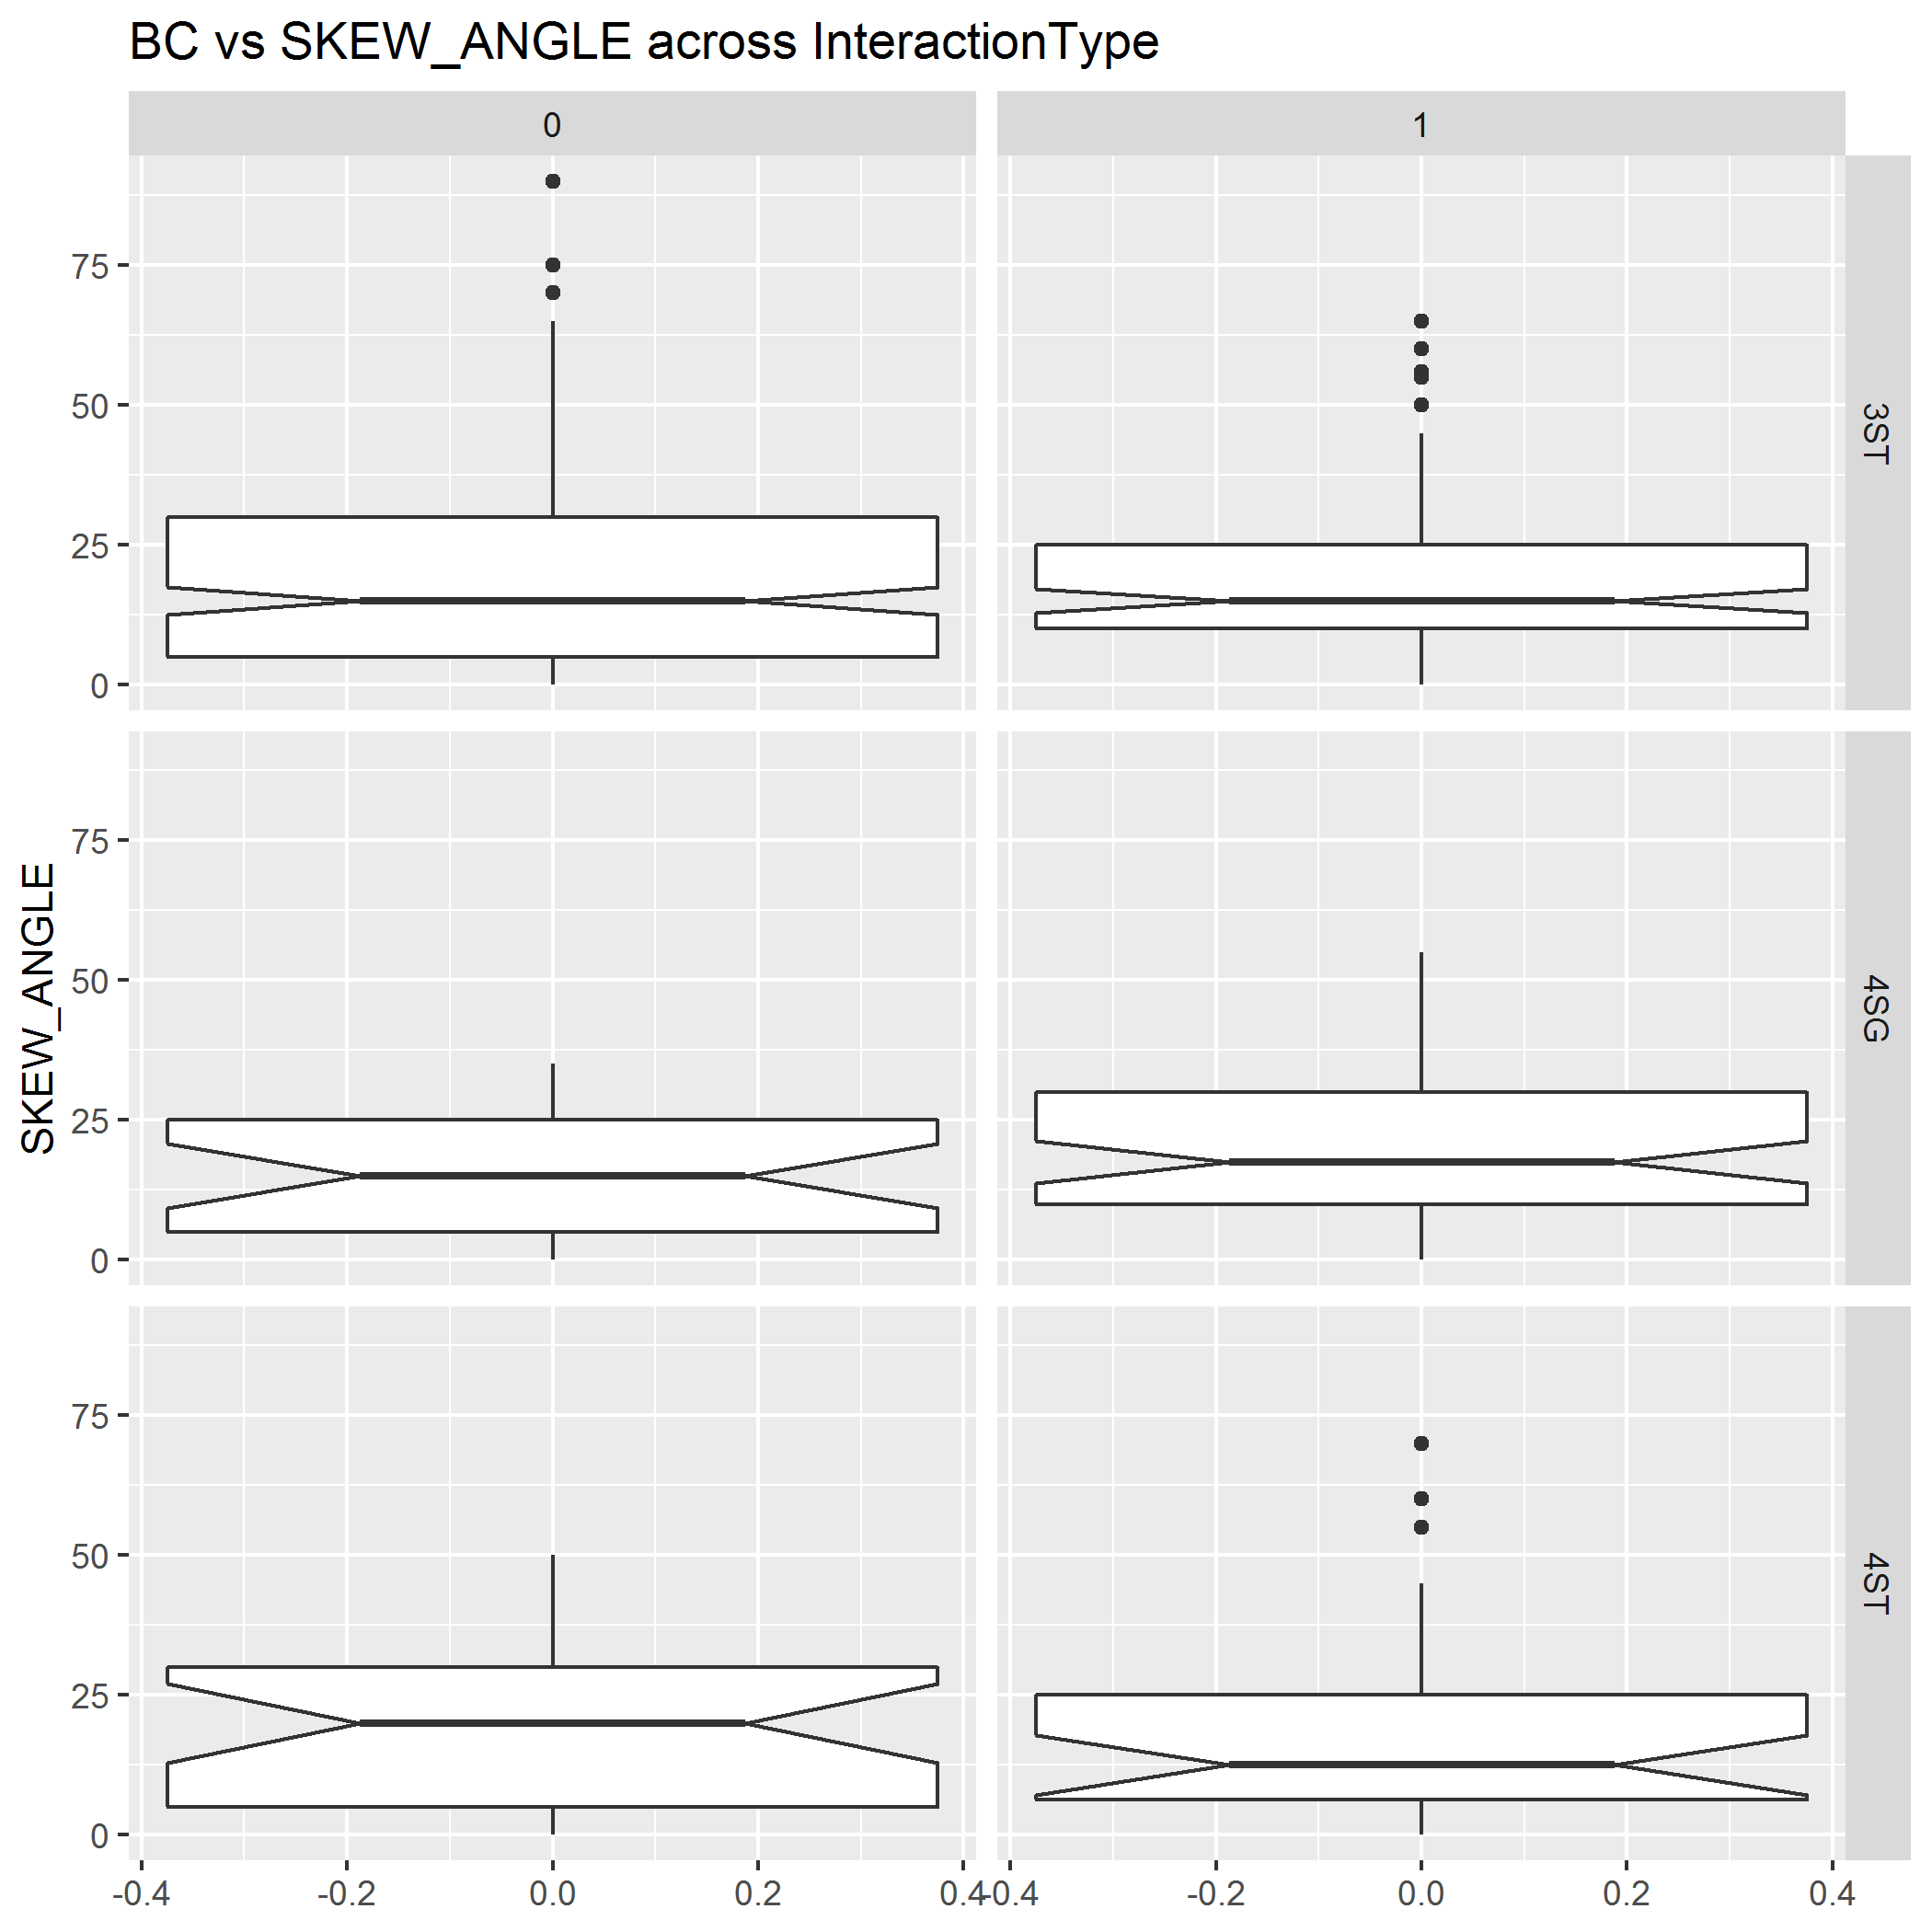
\includegraphics[width=3in]{image/extra12.png}
\small
\end{minipage}
\caption{Extra plots for Skew-Angle}
\end{figure}

Extra support plots for Lighting:
\begin{figure}[H]
\begin{minipage}[t]{0.5\linewidth}
\centering
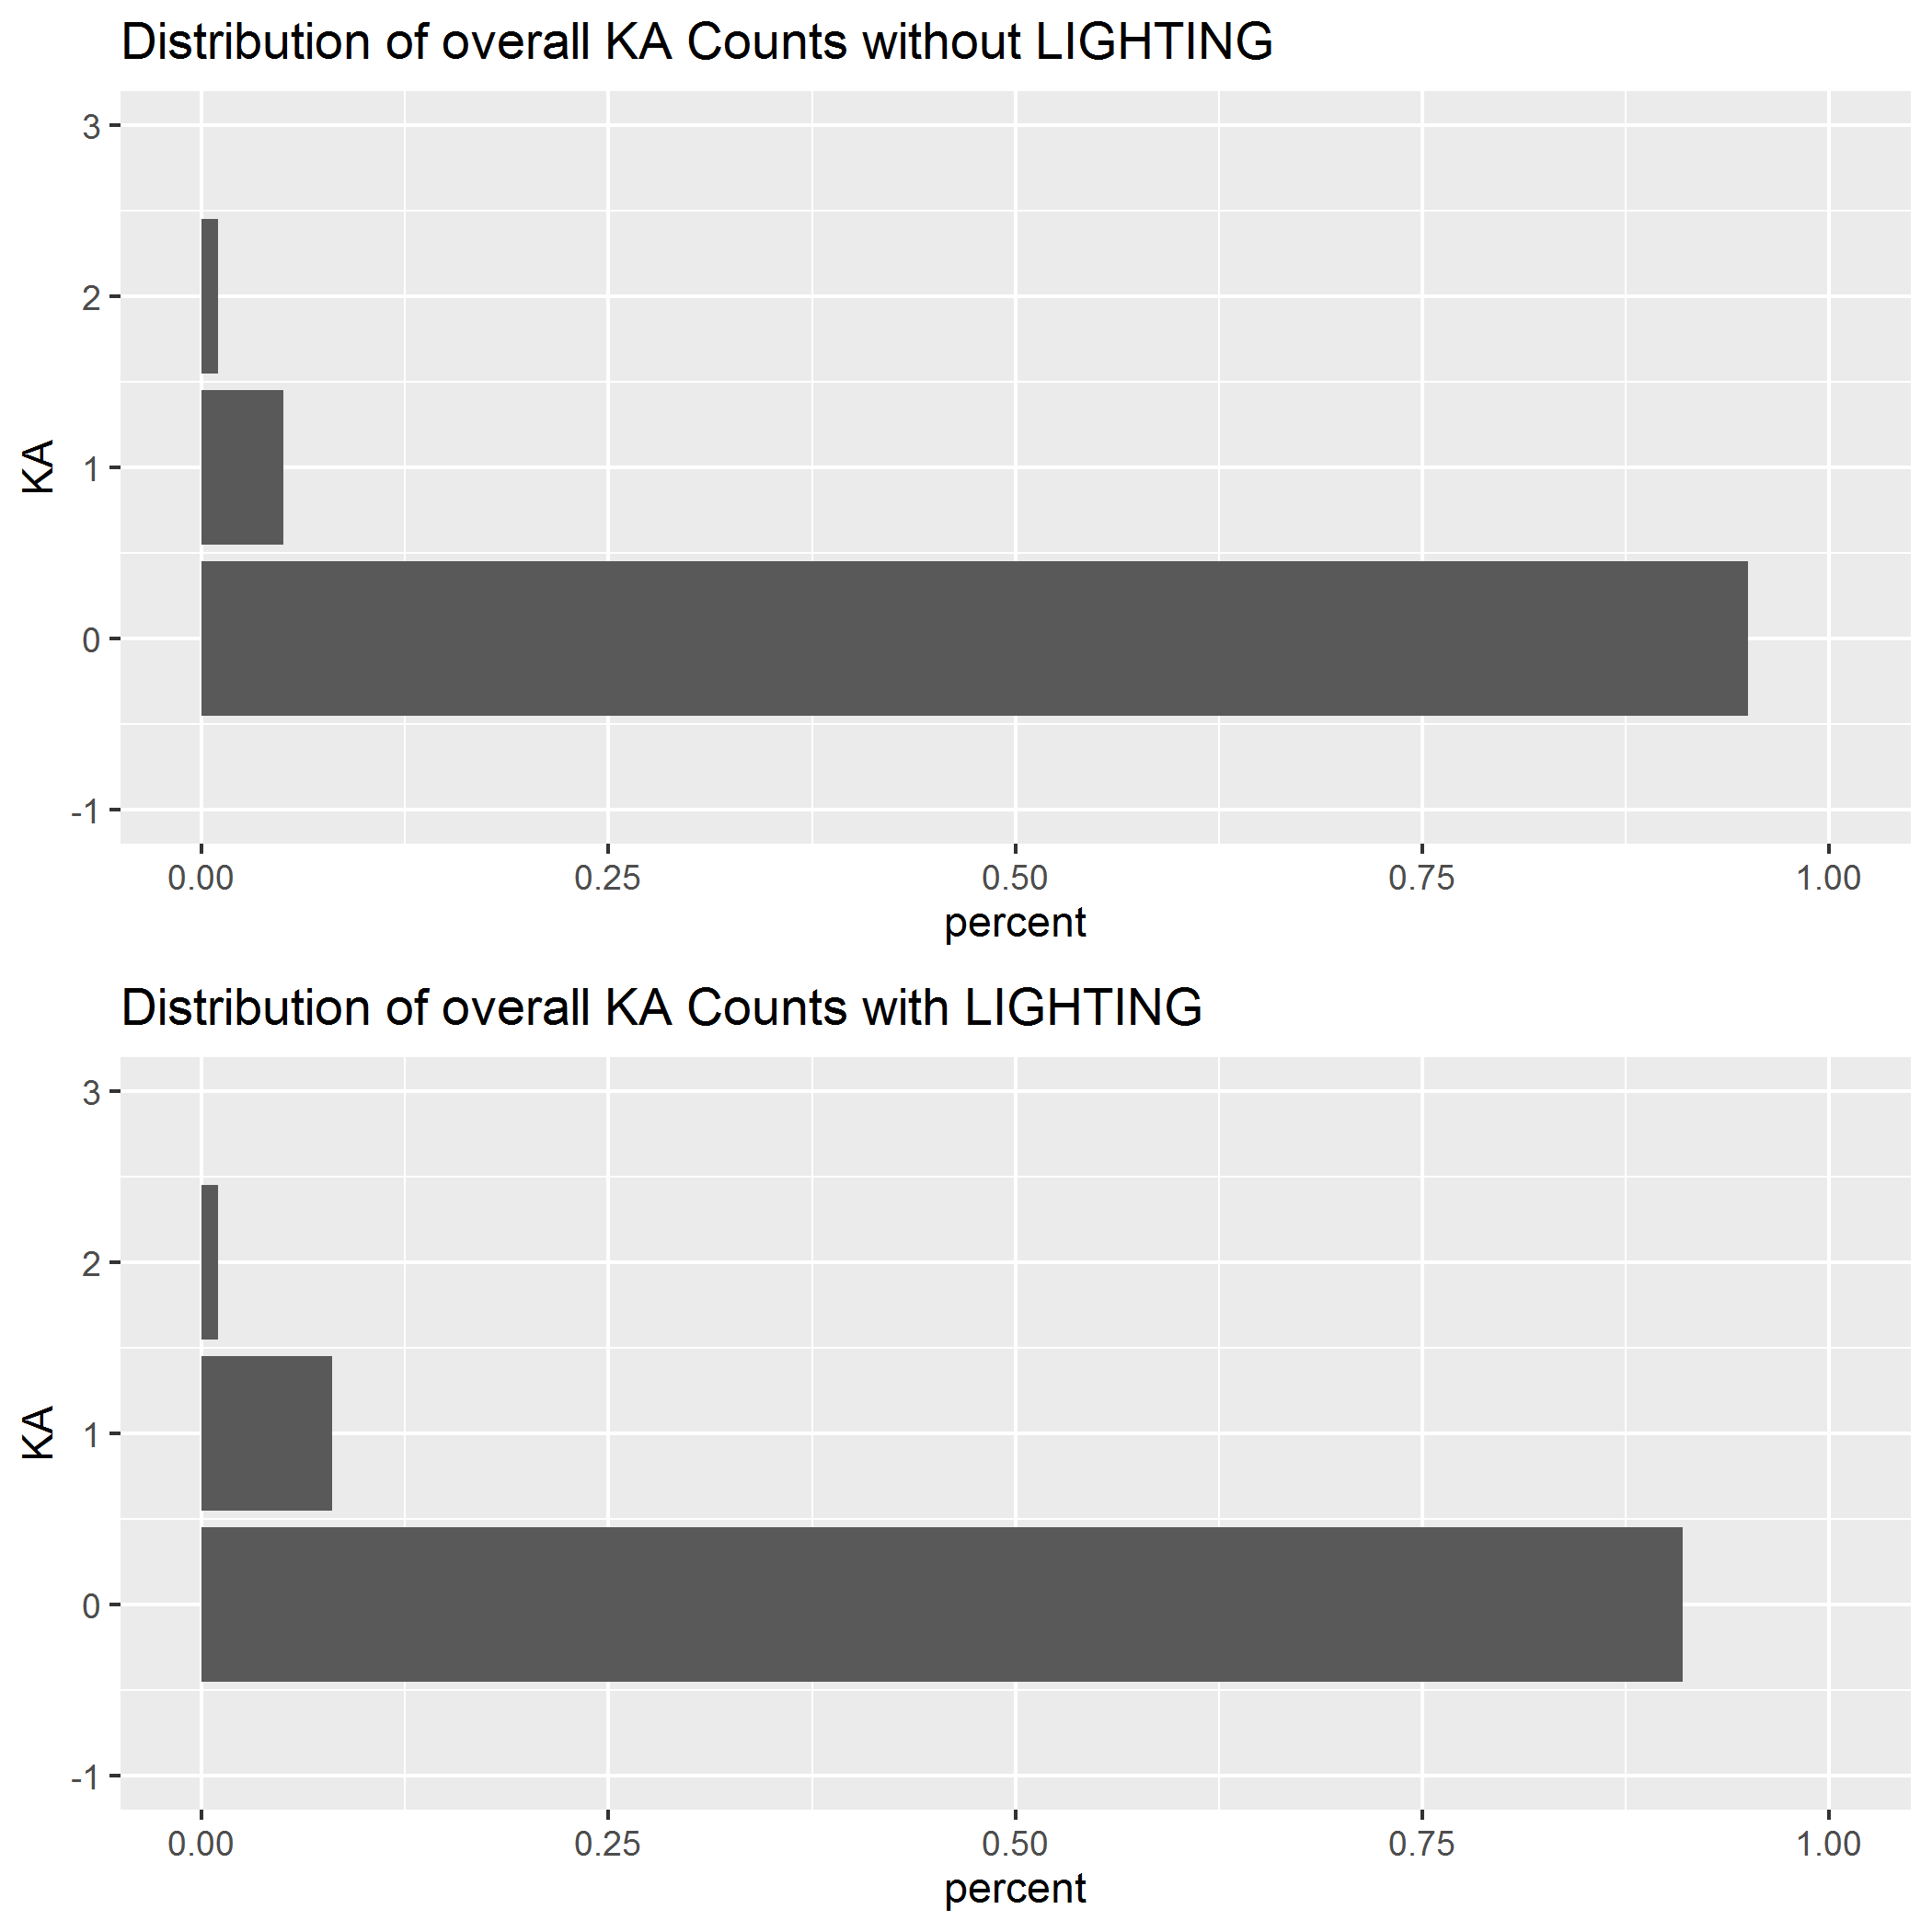
\includegraphics[width=3in]{image/LIGHTING_all_KA.png}
\small
\end{minipage}
\begin{minipage}[t]{0.5\linewidth}
\centering
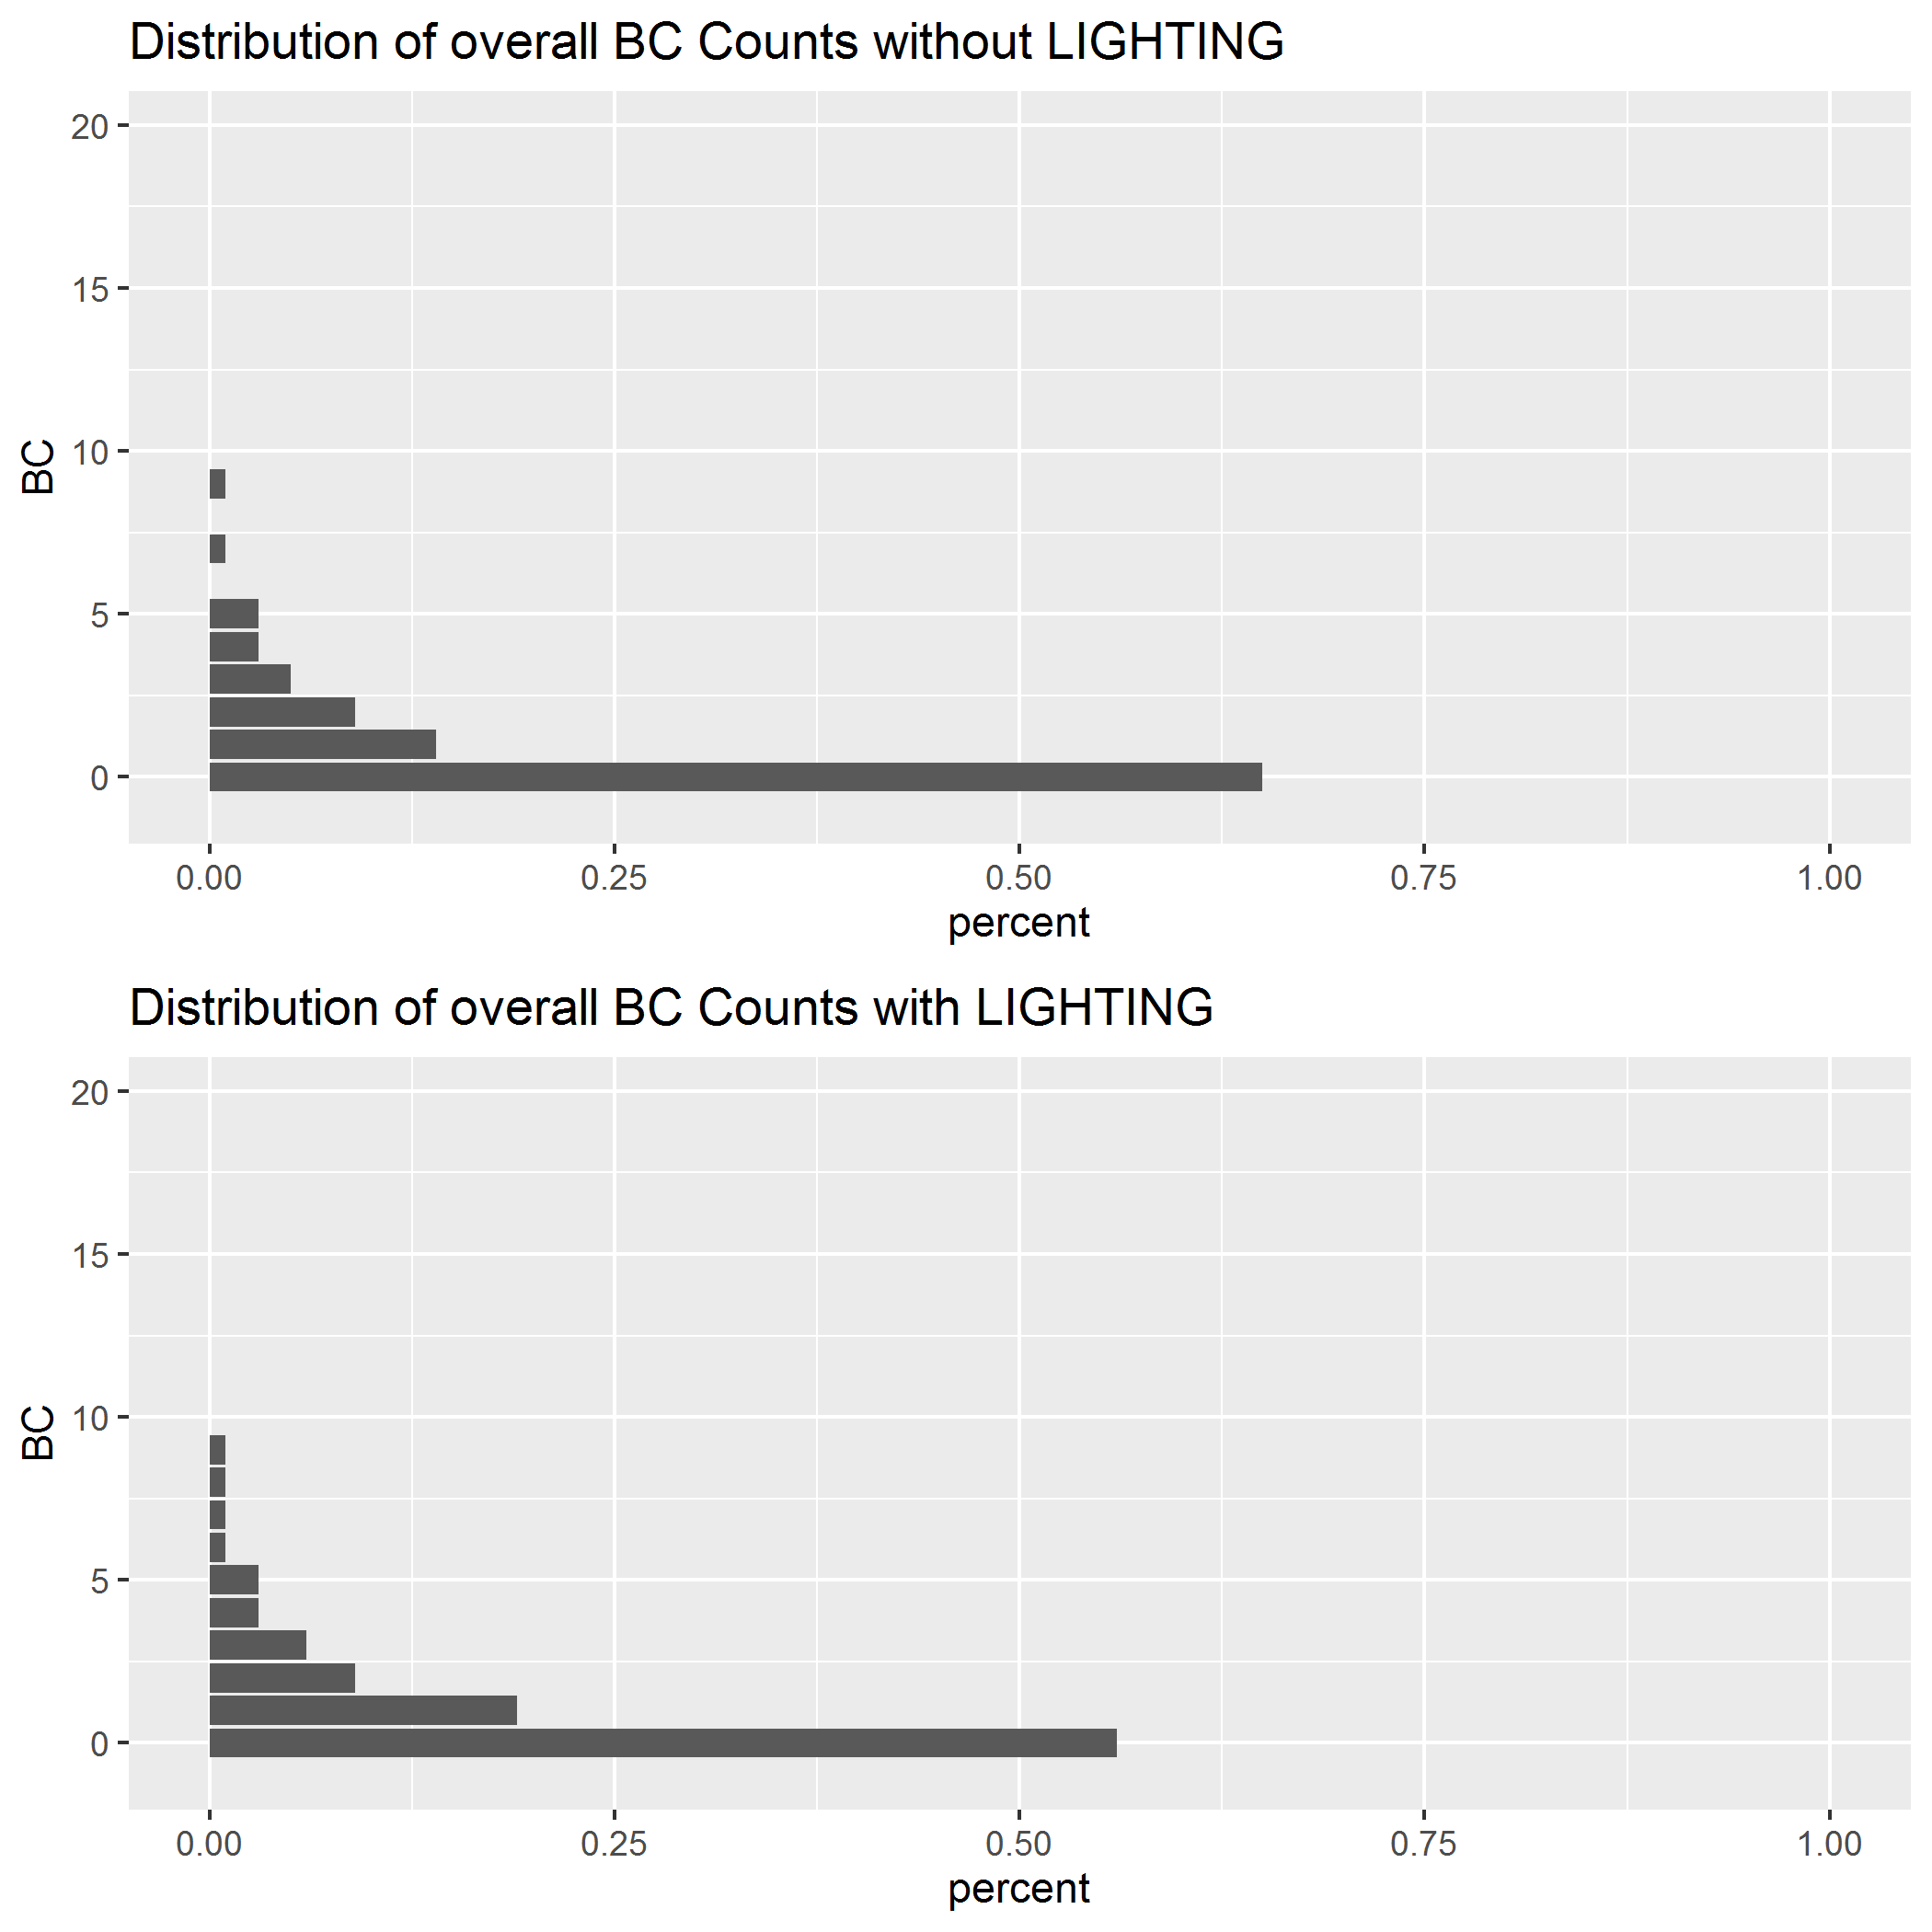
\includegraphics[width=3in]{image/LIGHTING_all_BC.png}
\small
\end{minipage}
\caption{Extra plots for Lighting}
\end{figure}


\subsection{R codes}

\subsubsection{EDA}
\lstset{language=R, breaklines=true}
\begin{lstlisting}
library(tidyverse)
library(gridExtra)
dat_1 = read.csv('./../data/3ST.csv')
dat_2 = read.csv('./../data/4ST.csv')
dat_3 = read.csv('./../data/4SG.csv')
dat_all = rbind(dat_1,dat_2,dat_3)
dat_all$INTERTYPE = c(rep('3ST',nrow(dat_1)),rep('4ST',nrow(dat_2)),rep('4SG',nrow(dat_3)))

## 1.1 Overall
##Overall distribution of 3 types of accidents: Use original counts, and group counts larger than 10 to be a single group. Make pie plots
### 1-1-1 PDO

cbPalette <- c("#999999", "#E69F00", "#56B4E9", "#009E73",
               "#F0E442","#0072B2","#D55E00","#CC79A7",
               "#000000","#330066","#CC9933","#006600",
               "#660033","#C1FFC1","#DCDCDC","#BDB76B","#FFD39B"
)

tab1 = table(dat_all$PDO)
over15 = sum(tab1[which(as.numeric(names(tab1))>15)])
tab1 = tab1[which(as.numeric(names(tab1))<=15)]
accidents = c(names(tab1),'over15')
accidents=factor(accidents,levels=c("0" ,"1", "2", "3", "4", "5", "6" ,"7" ,"8" ,"9", "10", "11", "12", "13", "15","over15"))
tab1 = data.frame(counts=c(as.vector(tab1),over15),accidents=accidents)
tab1 = tab1 %>% mutate(labels=
                         paste(accidents,"(",counts,"/",round(counts/sum(counts),2)*100,"%",")",sep=""))
p111 = ggplot(tab1,aes(x="",y=counts,fill=(accidents)))+
  geom_bar(stat='identity')+coord_polar("y")+
  scale_fill_manual(values =cbPalette,labels=tab1$labels)+
  theme(legend.text = element_text(size = 9),axis.text = element_blank())+
  ggtitle("Distribution of Number of Overall Annual PDO Counts")
png(file="./../../report/image/p1.png")
p111
dev.off()
### 1-1-2 KA
tab1 = table(dat_all$KA)
over15 = sum(tab1[which(as.numeric(names(tab1))>15)])
tab1 = tab1[which(as.numeric(names(tab1))<=15)]
accidents = c(names(tab1),'over15')
accidents=factor(accidents,levels=c(names(tab1),'over15'))
tab1 = data.frame(counts=c(as.vector(tab1),over15),accidents)
tab1 = tab1 %>% mutate(labels=
                         paste(accidents,"(",counts,"/",round(counts/sum(counts),2)*100,"%",")",sep=""))
p112 = ggplot(tab1,aes(x="factor(1)",y=counts,fill=accidents))+
  geom_bar(stat='identity')+coord_polar("y")+
  scale_fill_manual(values =cbPalette,labels=tab1$labels)+
  theme(legend.text = element_text(size = 10),axis.text = element_blank())+
  ggtitle("Distribution of Number of Overall Annual KA Counts")
png(file="./../../report/image/p112.png")
p112
dev.off()
### 1-1-3 BC
tab1 = table(dat_all$BC)
over15 = sum(tab1[which(as.numeric(names(tab1))>15)])
tab1 = tab1[which(as.numeric(names(tab1))<=15)]
accidents = c(names(tab1),'over15')
accidents=factor(accidents,levels=c(names(tab1),'over15'))
tab1 = data.frame(counts=c(as.vector(tab1),over15),accidents)
tab1 = tab1 %>% mutate(labels=
                         paste(accidents,"(",counts,"/",round(counts/sum(counts),2)*100,"%",")",sep=""))
p113 = ggplot(tab1,aes(x="factor(1)",y=counts,fill=accidents))+
  geom_bar(stat='identity')+coord_polar("y")+
  scale_fill_manual(values =cbPalette,labels=tab1$labels)+
  theme(legend.text = element_text(size = 10),axis.text = element_blank())+
  ggtitle("Distribution of Number of Overall Annual BC Counts")
png(file="./../../report/image/p113.png")
p113
dev.off()

## 1.2 Accident counts VS variables

### 1-2-1 Accident across interaction type
datplot = dat_all
datplot$PDO[which(datplot$PDO>15)] = 'over15'
datplot$PDO=factor(datplot$PDO,levels=c(as.character(0:15),'over15'))
p121_PDO = ggplot(datplot,aes(x=factor(1),fill=PDO))+
  geom_bar(position = 'fill')+
  coord_polar("y")+
  scale_fill_manual(values =cbPalette )+
  facet_wrap(~INTERTYPE)+
  theme(legend.text = element_text(size = 10),
        axis.text = element_blank(),
        legend.position = 'top',
        legend.title=element_text(size=10))+
  ggtitle("Distribution of PDO Counts over InteractionType")
png(file="./../../report/image/p121_PDO.png")
p121_PDO
dev.off()
#KA
datplot = dat_all
datplot$KA[which(datplot$KA>15)] = 'over15'
datplot$PDO=factor(datplot$PDO,levels=c(as.character(0:15),'over15'))
p121_KA = ggplot(datplot,aes(x=factor(1),fill=KA))+
  geom_bar(position = 'fill')+
  coord_polar("y")+
  scale_fill_manual(values =cbPalette )+
  facet_wrap(~INTERTYPE)+
  theme(legend.text = element_text(size = 10),
        axis.text = element_blank(),
        legend.position = 'top',
        legend.title=element_text(size=10))+
  ggtitle("Distribution of KA Counts over InteractionType")
png(file="./../../report/image/p121_KA.png")
p121_KA
dev.off()
#BC
datplot = dat_all
datplot$BC[which(datplot$BC>15)] = 'over15'
datplot$PDO=factor(datplot$PDO,levels=c(as.character(0:15),'over15'))
p121_BC = ggplot(datplot,aes(x=factor(1),fill=BC))+
  geom_bar(position = 'fill')+
  coord_polar("y")+
  scale_fill_manual(values =cbPalette )+
  facet_wrap(~INTERTYPE)+
  theme(legend.text = element_text(size = 10),
        axis.text = element_blank(),
        legend.position = 'top',
        legend.title=element_text(size=10))+
  ggtitle("Distribution of BC Counts over InteractionType")
png(file="./../../report/image/p121_BC.png")
p121_BC
dev.off()
### 1-2-2 Accident VS AADT-MAJOR
g1 = dat_all %>% ggplot(aes(AADT_MAJOR,AADT_MINOR))+geom_point()+
  geom_smooth(method='lm')+ggtitle('Relationship between AADT-Major and AADT-Minor')+facet_grid(~INTERTYPE)
ggsave(file="./../../report/image/major_minor.png", g1)
cor(dat_all$AADT_MAJOR,dat_all$AADT_MINOR)
dat_all%>% group_by(INTERTYPE) %>% summarise(r=cor(AADT_MAJOR,AADT_MINOR))
##overall
p122_overall_pdo = dat_all %>% mutate(PDO_ACCIDENT=as.numeric(PDO>0)) %>%
  ggplot(aes(y=AADT_MAJOR))+geom_boxplot(notch=TRUE)+facet_grid(.~PDO_ACCIDENT)+ggtitle("PDO vs AADT_MAJOR")
ggsave(file="./../../report/image/major_all_pdo.png", p122_overall_pdo)

p122_overall_ka = dat_all %>% mutate(PDO_ACCIDENT=as.numeric(KA>0)) %>%
  ggplot(aes(y=AADT_MAJOR))+geom_boxplot(notch=TRUE)+facet_grid(.~PDO_ACCIDENT)+ggtitle("KA vs AADT_MAJOR")

p122_overall_bc = dat_all %>% mutate(PDO_ACCIDENT=as.numeric(BC>0)) %>%
  ggplot(aes(y=AADT_MAJOR))+geom_boxplot(notch=TRUE)+facet_grid(.~PDO_ACCIDENT)+ggtitle("BC vs AADT_MAJOR")


Across interaction type

p122_pdo = dat_all %>% mutate(PDO_ACCIDENT=as.numeric(PDO>0)) %>%
  ggplot(aes(y=AADT_MAJOR))+geom_boxplot(notch=TRUE)+facet_grid(INTERTYPE~PDO_ACCIDENT)+ggtitle("PDO vs AADT_MAJOR across InteractionType")

p122_ka = dat_all %>% mutate(PDO_ACCIDENT=as.numeric(KA>0)) %>%
  ggplot(aes(y=AADT_MAJOR))+geom_boxplot(notch=TRUE)+facet_grid(INTERTYPE~PDO_ACCIDENT)+ggtitle("KA vs AADT_MAJOR across InteractionType")
ggsave(file="./../../report/image/major_ka.png", p122_ka)

p122_bc = dat_all %>% mutate(PDO_ACCIDENT=as.numeric(BC>0)) %>%
  ggplot(aes(y=AADT_MAJOR))+geom_boxplot(notch=TRUE)+facet_grid(INTERTYPE~PDO_ACCIDENT)+ggtitle("BC vs AADT_MAJOR across InteractionType")
ggsave(file="./../../report/image/major_bc.png", p122_bc)
### 1-2-3 Accident VS AADT-MINOR
p123_overall_pdo = dat_all %>% mutate(PDO_ACCIDENT=as.numeric(PDO>0)) %>%
  ggplot(aes(y=AADT_MINOR))+geom_boxplot(notch=TRUE)+facet_grid(.~PDO_ACCIDENT)+ggtitle("PDO vs AADT_MINOR")
ggsave(file="./../../report/image/minor_all_pdo.png", p123_overall_pdo)

p123_overall_ka = dat_all %>% mutate(PDO_ACCIDENT=as.numeric(KA>0)) %>%
  ggplot(aes(y=AADT_MINOR))+geom_boxplot(notch=TRUE)+facet_grid(.~PDO_ACCIDENT)+ggtitle("KA vs AADT_MINOR")

p123_overall_bc = dat_all %>% mutate(PDO_ACCIDENT=as.numeric(BC>0)) %>%
  ggplot(aes(y=AADT_MINOR))+geom_boxplot(notch=TRUE)+facet_grid(.~PDO_ACCIDENT)+ggtitle("BC vs AADT_MINOR")


#Across interaction type

P123_pdo = dat_all %>% mutate(PDO_ACCIDENT=as.numeric(PDO>0)) %>%
  ggplot(aes(y=AADT_MINOR))+geom_boxplot(notch=TRUE)+facet_grid(INTERTYPE~PDO_ACCIDENT)+ggtitle("PDO vs AADT_MINOR across InteractionType")
ggsave(file="./../../report/image/minor_pdo.png", P123_pdo)

P123_ka = dat_all %>% mutate(PDO_ACCIDENT=as.numeric(KA>0)) %>%
  ggplot(aes(y=AADT_MINOR))+geom_boxplot(notch=TRUE)+facet_grid(INTERTYPE~PDO_ACCIDENT)+ggtitle("KA vs AADT_MINOR across InteractionType")

P123_bc = dat_all %>% mutate(PDO_ACCIDENT=as.numeric(BC>0)) %>%
  ggplot(aes(y=AADT_MINOR))+geom_boxplot(notch=TRUE)+facet_grid(INTERTYPE~PDO_ACCIDENT)+ggtitle("BC vs AADT_MINOR across InteractionType")

### 1-2-4 Accident VS SKEW-ANGLE
#overall
p123_overall_pdo = dat_all %>% mutate(PDO_ACCIDENT=as.numeric(PDO>0)) %>%
  ggplot(aes(y=SKEW_ANGLE))+geom_boxplot(notch=TRUE)+facet_grid(.~PDO_ACCIDENT)+ggtitle("PDO vs SKEW_ANGLE")
ggsave(file="./../../report/image/angle_all_pdo.png", p123_overall_pdo)

p123_overall_ka = dat_all %>% mutate(PDO_ACCIDENT=as.numeric(KA>0)) %>%
  ggplot(aes(y=SKEW_ANGLE))+geom_boxplot(notch=TRUE)+facet_grid(.~PDO_ACCIDENT)+ggtitle("KA vs SKEW_ANGLE")

p123_overall_bc = dat_all %>% mutate(PDO_ACCIDENT=as.numeric(BC>0)) %>%
  ggplot(aes(y=SKEW_ANGLE))+geom_boxplot(notch=TRUE)+facet_grid(.~PDO_ACCIDENT)+ggtitle("BC vs SKEW_ANGLE")

#Across interaction type
p123_pdo = dat_all %>% mutate(PDO_ACCIDENT=as.numeric(PDO>0)) %>%
  ggplot(aes(y=SKEW_ANGLE))+geom_boxplot(notch=TRUE)+facet_grid(INTERTYPE~PDO_ACCIDENT)+ggtitle("PDO vs SKEW_ANGLE across InteractionType")
ggsave(file="./../../report/image/angle_pdo.png", p123_pdo)

p123_ka = dat_all %>% mutate(PDO_ACCIDENT=as.numeric(KA>0)) %>%
  ggplot(aes(y=SKEW_ANGLE))+geom_boxplot(notch=TRUE)+facet_grid(INTERTYPE~PDO_ACCIDENT)+ggtitle("KA vs SKEW_ANGLE across InteractionType")

p123_bc = dat_all %>% mutate(PDO_ACCIDENT=as.numeric(BC>0)) %>%
  ggplot(aes(y=SKEW_ANGLE))+geom_boxplot(notch=TRUE)+facet_grid(INTERTYPE~PDO_ACCIDENT)+ggtitle("BC vs SKEW_ANGLE across InteractionType")

### 1-2-5 Accident VS lighting
dat_all$crash = as.numeric((dat_all$PDO+dat_all$BC+dat_all$KA)>0)
getcatgraph <- function(v,crash){
  if(crash=='PDO'){a=25;b=0.5}
  if(crash=='KA'){a=3;b=1}
  if(crash=='BC'){a=20;b=1}
  if(crash=='crash'){a=2;b=1}
  g1 = dat_all %>% filter(!!sym(v)==0) %>% group_by(!!sym(crash)) %>% summarise(count=n()) %>% mutate(percent=round(count/sum(count),2)) %>% ggplot(aes(x=!!sym(crash),y=percent))+
    geom_bar(stat='identity')+coord_flip()+xlim(c(-1,a))+ylim(c(0,b))+
    ggtitle(c(paste("Distribution of overall",as.character(crash),"Counts without",as.character(v))))
  g2 = dat_all %>% filter(!!sym(v)==1) %>% group_by(!!sym(crash)) %>% summarise(count=n()) %>% mutate(percent=round(count/sum(count),2)) %>% ggplot(aes(x=!!sym(crash),y=percent))+
    geom_bar(stat='identity')+coord_flip()+xlim(c(-1,a))+ylim(c(0,b))+
    ggtitle(c(paste("Distribution of overall",as.character(crash),"Counts with",as.character(v))))

  g <- arrangeGrob(g1,g2,nrow=2)
  ggsave(file=paste("./../../report/image/",as.character(v),"_all_",as.character(crash),".png",sep=""), g)


  g1 = dat_all %>% filter(!!sym(v)==0,INTERTYPE=='3ST') %>% group_by(!!sym(crash)) %>% summarise(count=n()) %>% mutate(percent=round(count/sum(count),2)) %>% ggplot(aes(x=!!sym(crash),y=percent))+
    geom_bar(stat='identity')+coord_flip()+xlim(c(-1,a))+ylim(c(0,b))+
    ggtitle(paste("Distribution of 3ST",as.character(crash),"Counts without",as.character(v)))
  g2 = dat_all %>% filter(!!sym(v)==1,INTERTYPE=='3ST') %>% group_by(!!sym(crash)) %>% summarise(count=n()) %>% mutate(percent=round(count/sum(count),2)) %>% ggplot(aes(x=!!sym(crash),y=percent))+
    geom_bar(stat='identity')+coord_flip()+xlim(c(-1,a))+ylim(c(0,b))+
    ggtitle(paste("Distribution of 3ST",as.character(crash),"Counts with",as.character(v)))

  g <- arrangeGrob(g1,g2,nrow=2)
  ggsave(file=paste("./../../report/image/",v,"_3ST_",crash,".png",sep=""), g)

  g1 = dat_all %>% filter(!!sym(v)==0,INTERTYPE=='4ST') %>% group_by(!!sym(crash)) %>% summarise(count=n()) %>% mutate(percent=round(count/sum(count),2)) %>% ggplot(aes(x=!!sym(crash),y=percent))+
    geom_bar(stat='identity')+coord_flip()+xlim(c(-1,a))+ylim(c(0,b))+
    ggtitle(paste("Distribution of 4ST",crash,"Counts without",v))
  g2 = dat_all %>% filter(!!sym(v)==1,INTERTYPE=='4ST') %>% group_by(!!sym(crash)) %>% summarise(count=n()) %>% mutate(percent=round(count/sum(count),2)) %>% ggplot(aes(x=!!sym(crash),y=percent))+
    geom_bar(stat='identity')+coord_flip()+xlim(c(-1,a))+ylim(c(0,b))+
    ggtitle(paste("Distribution of 4ST",crash,"Counts with",v))

  g <- arrangeGrob(g1,g2,nrow=2)
  ggsave(file=paste("./../../report/image/",v,"_4ST_",crash,".png",sep=""), g)

  g1 = dat_all %>% filter(!!sym(v)==0,INTERTYPE=='4SG') %>% group_by(!!sym(crash)) %>% summarise(count=n()) %>% mutate(percent=round(count/sum(count),2)) %>% ggplot(aes(x=!!sym(crash),y=percent))+
    geom_bar(stat='identity')+coord_flip()+xlim(c(-1,a))+ylim(c(0,b))+
    ggtitle(paste("Distribution of 4SG",crash,"Counts without",v))
  g2 = dat_all %>% filter(!!sym(v)==1,INTERTYPE=='4SG') %>% group_by(!!sym(crash)) %>% summarise(count=n()) %>% mutate(percent=round(count/sum(count),2)) %>% ggplot(aes(x=!!sym(crash),y=percent))+
    geom_bar(stat='identity')+coord_flip()+xlim(c(-1,a))+ylim(c(0,b))+
    ggtitle(paste("Distribution of 4SG",crash,"Counts with",v))

  g <- arrangeGrob(g1,g2,nrow=2)
  ggsave(file=paste("./../../report/image/",v,"_4SG_",crash,".png",sep=""), g)

}
getcatgraph("LIGHTING","PDO")
getcatgraph("LIGHTING","KA")
getcatgraph("LIGHTING","BC")
table(dat_all$LIGHTING)
### 1-2-6 Accident VS APPROACHLEFT_TURN

table(dat_all$APPROACH_LEFTTURN,dat_all$INTERTYPE)
getcatgraph("APPROACH_LEFTTURN","PDO")
# too less obs in PDO 4ST
getcatgraph("APPROACH_LEFTTURN","KA")
getcatgraph("APPROACH_LEFTTURN","BC")

# not partitioned by crashtype
g1 = dat_all %>% mutate(APPROACH_LEFTTURN=as.character(APPROACH_LEFTTURN)) %>%
  group_by(APPROACH_LEFTTURN,INTERTYPE) %>%
  summarise(crash_percent = mean(crash)) %>%
  ggplot(aes(x=APPROACH_LEFTTURN,y=crash_percent,fill=APPROACH_LEFTTURN))+geom_bar(stat='identity')+
  facet_grid(~INTERTYPE)+ggtitle('Distribution of Crash-rate over Approach Left-Turn across Intersection Type')
ggsave(file="./../../report/image/approach-left-turn.png", g1)

g1 = dat_all %>% mutate(APPROACH_LEFTTURN=as.character(APPROACH_LEFTTURN)) %>%
  group_by(APPROACH_LEFTTURN) %>%
  summarise(crash_percent = mean(crash)) %>%
  ggplot(aes(x=APPROACH_LEFTTURN,y=crash_percent,fill=APPROACH_LEFTTURN))+geom_bar(stat='identity')+ggtitle('Overall Distribution of Crash-rate over Approach Left-Turn')
ggsave(file="./../../report/image/approach-left-turn-all.png", g1)

### 1-2-6 Accident VS APPROACHLEFTTRUE
table(dat_all$APPROACH_RIGHTTURN,dat_all$INTERTYPE)
getcatgraph("APPROACH_RIGHTTURN","PDO")
# too less obs in PDO 4ST
getcatgraph("APPROACH_RIGHTTURN","KA")
getcatgraph("APPROACH_RIGHTTURN","BC")

# not partitioned by crashtype
g1 = dat_all %>% mutate(APPROACH_RIGHTTURN=as.character(APPROACH_RIGHTTURN)) %>%
  group_by(APPROACH_RIGHTTURN,INTERTYPE) %>%
  summarise(crash_percent = mean(crash)) %>%
  ggplot(aes(x=APPROACH_RIGHTTURN,y=crash_percent,fill=APPROACH_RIGHTTURN))+geom_bar(stat='identity')+
  facet_grid(~INTERTYPE)+ggtitle('Distribution of Crash-rate over Approach Right-Turn across Intersection Type')
ggsave(file="./../../report/image/approach-right-turn.png", g1)

g1 = dat_all %>% mutate(APPROACH_RIGHTTURN=as.character(APPROACH_RIGHTTURN)) %>%
  group_by(APPROACH_RIGHTTURN) %>%
  summarise(crash_percent = mean(crash)) %>%
  ggplot(aes(x=APPROACH_RIGHTTURN,y=crash_percent,fill=APPROACH_RIGHTTURN))+geom_bar(stat='identity')+ggtitle('Overall Distribution of Crash-rate over Approach Right-Turn')
ggsave(file="./../../report/image/approach-right-turn-all.png", g1)
### 1-2-7 Accident VS APPROATRUE
dat_all$turn = as.numeric(dat_all$APPROACH_LEFTTURN+dat_all$APPROACH_RIGHTTURN>0)
table(dat_all$turn,dat_all$INTERTYPE)

# not partitioned by crashtype
g1 = dat_all %>% mutate(turn=as.character(turn)) %>%
  group_by(turn,INTERTYPE) %>%
  summarise(crash_percent = mean(crash)) %>%
  ggplot(aes(x=turn,y=crash_percent,fill=turn))+geom_bar(stat='identity')+
  facet_grid(~INTERTYPE)+ggtitle('Distribution of Crash-rate over Approach Turn across Intersection Type')
ggsave(file="./../../report/image/approach-turn.png", g1)

g1 = dat_all %>% mutate(turn=as.character(turn)) %>%
  group_by(turn) %>%
  summarise(crash_percent = mean(crash)) %>%
  ggplot(aes(x=turn,y=crash_percent,fill=turn))+geom_bar(stat='identity')+ggtitle('Overall Distribution of Crash-rate over Approach Turn')
ggsave(file="./../../report/image/approach-turn-all.png", g1)

\end{lstlisting}

\subsubsection{Inference}
\begin{lstlisting}
\lstset{language=R, breaklines=true}
##Data import
dat_1 = read.csv('./../data/3ST.csv')
dat_2 = read.csv('./../data/4ST.csv')
dat_3 = read.csv('./../data/4SG.csv')

### Question 1: Simplest question, do these different types of intersection holds different number of crashes? (Measured by mean or median.)

### About PDO

st3_pdo = dat_1$PDO
st4_pdo = dat_2$PDO
sg4_pdo = dat_3$PDO

### Check same dispersion assumption for Mann Whitney test: only st4 vs sg4 group satisfied

ansari.test(st3_pdo,st4_pdo)
ansari.test(st4_pdo,sg4_pdo)
ansari.test(st3_pdo,sg4_pdo)

### Check st3_pdo with st4_pdo:

library(magrittr)
X <- data.frame(value = data.matrix(st3_pdo), label = "st3")
Y <- data.frame(value = data.matrix(st4_pdo), label = "st4")
data_XY <- rbind(X,Y)[order(rbind(X,Y)$value),]
data_XY$rank = rank(data_XY$value, ties.method = "average")
table(data_XY$rank)
W <- data_XY[data_XY$label=='st4',] %>% dplyr::select("rank") %>% sum
n = length(st4_pdo)
m = length(st3_pdo)
E_0_W <- n *(m+n+1)/2
var_0_W <- (m*n/12)*((m+n+1)-1/((m+n)*(m+n-1))*(191*(191^2-1)+78*(78^2-1)+61*(61^2-1)+32*(32^2-1)+25*(25^2-1)+17*(17^2-1)+10*(10^2-1)+7*(7^2-1)+9*(9^2-1)+6*(6^2-1)+2*(2^2-1)+3*(3^2-1)))
T_ <- abs((W-E_0_W)/sqrt(var_0_W))
Z_crit <- qnorm(0.025, 0, 1, lower.tail = F)
abs(T_) > Z_crit

### Check by 95% boostrap CI. 95% confident CI does not contain 0 and both bounds are negative
bootci <- function(x,y){
  n1 = length(x)
  n2 = length(y)
  dif = NULL
  for(i in 1:1000){
    x1 = base::sample(x,n1,replace=TRUE)
    x2 = base::sample(y,n2,replace=TRUE)
    dif = c(dif, mean(x1)-mean(x2))
  }
  return(quantile(dif,prob=c(0.025,0.975)))
}
set.seed(1)
bootci(st3_pdo,st4_pdo)

### It returns true, so we think there is difference.

### Check st4_pdo with sg4_pdo:

X <- data.frame(value = data.matrix(st4_pdo), label = "st4")
Y <- data.frame(value = data.matrix(sg4_pdo), label = "sg4")
data_XY <- rbind(X,Y)[order(rbind(X,Y)$value),]
data_XY$rank = rank(data_XY$value, ties.method = "average")
table(data_XY$rank)
W <- data_XY[data_XY$label=='sg4',] %>% dplyr::select("rank") %>% sum
n = length(sg4_pdo)
m = length(st4_pdo)
E_0_W <- n *(m+n+1)/2
var_0_W <- (m*n/12)*((m+n+1)-1/((m+n)*(m+n-1))*(36*(36^2-1)+13*(13^2-1)+12*(12^2-1)+16*(16^2-1)+10*(10^2-1)+8*(8^2-1)+13*(13^2-1)+10*(10^2-1)+9*(9^2-1)+2*(2^2-1)+3*(3^2-1)+2*(2^2-1)+5*(5^2-1)+2*3*(3^2-1)+2*(2^2-1)))
T_ <- abs((W-E_0_W)/sqrt(var_0_W))
Z_crit <- qnorm(0.025, 0, 1, lower.tail = F)
abs(T_) > Z_crit

### Also return true, so we think there is difference.

### Check st3_pdo with sg4_pdo:

X <- data.frame(value = data.matrix(st3_pdo), label = "st3")
Y <- data.frame(value = data.matrix(sg4_pdo), label = "sg4")
data_XY <- rbind(X,Y)[order(rbind(X,Y)$value),]
data_XY$rank = rank(data_XY$value, ties.method = "average")
table(data_XY$rank)
W <- data_XY[data_XY$label=='sg4',] %>% dplyr::select("rank") %>% sum
n = length(sg4_pdo)
m = length(st3_pdo)
E_0_W <- n *(m+n+1)/2
var_0_W <- (m*n/12)*((m+n+1)-1/((m+n)*(m+n-1))*(191*(191^2-1)+75*(75^2-1)+53*(53^2-1)+30*(30^2-1)+27*(27^2-1)+23*(23^2-1)+19*(19^2-1)+2*13*(13^2-1)+9*(9^2-1)+3*2*(2^2-1)+4*(4^2-1)+5*(5^2-1)+6*(6^2-1)+2*3*(3^2-1)))
T_ <- abs((W-E_0_W)/sqrt(var_0_W))
Z_crit <- qnorm(0.025, 0, 1, lower.tail = F)
abs(T_) > Z_crit

### Also return true, so we think there is difference.

### Check by 95% boostrap CI. 95% confident CI does not contain 0 and both bounds are negative
set.seed(1)
bootci(st3_pdo,sg4_pdo)


### next, we use the categorical analysis perspective to verify the independence holds false.

st3_crash = c(nrow(dat_1[dat_1$PDO==0,]),nrow(dat_1[dat_1$PDO>0,]),nrow(dat_1[dat_1$PDO==0,])+nrow(dat_1[dat_1$PDO>0,]))
st4_crash = c(nrow(dat_2[dat_2$PDO==0,]),nrow(dat_2[dat_2$PDO>0,]),nrow(dat_2[dat_2$PDO==0,])+nrow(dat_2[dat_2$PDO>0,]))
sg4_crash = c(nrow(dat_3[dat_3$PDO==0,]),nrow(dat_3[dat_3$PDO>0,]),nrow(dat_3[dat_3$PDO==0,])+nrow(dat_3[dat_3$PDO>0,]))
total = st3_crash + st4_crash + sg4_crash
tbl <- data.frame(st3_crash,st4_crash,sg4_crash,total)
rownames(tbl) <- c('Safe',"Crash","total")
tbl
Q = 0
for (i in 1:2){
  for (j in 1:3){
    Q = Q + (tbl[i,j]-(tbl[i,4]*tbl[3,j]/tbl[3,4]))^2/(tbl[i,4]*tbl[3,j]/tbl[3,4])
  }
}
Q >= qchisq(0.95,df=(2*1))

### We get the same result: intersection type and DPO crash number are relative.

### About KA

st3_ka = dat_1$KA
st4_ka = dat_2$KA
sg4_ka = dat_3$KA

### Check same dispersion assumption for Mann Whitney test

ansari.test(st3_ka,st4_ka)
ansari.test(st4_ka,sg4_ka)
ansari.test(st3_ka,sg4_ka)

### Check st3_ka with st4_ka:

X <- data.frame(value = data.matrix(st3_ka), label = "st3")
Y <- data.frame(value = data.matrix(st4_ka), label = "st4")
data_XY <- rbind(X,Y)[order(rbind(X,Y)$value),]
data_XY$rank = rank(data_XY$value, ties.method = "average")
table(data_XY$rank)
W <- data_XY[data_XY$label=='st4',] %>% dplyr::select("rank") %>% sum
n = length(st4_ka)
m = length(st3_ka)
E_0_W <- n *(m+n+1)/2
var_0_W <- (m*n/12)*((m+n+1)-1/((m+n)*(m+n-1))*(425*(425^2-1)+19*(19^2-1)+2*(2^2-1)))
T_ <- abs((W-E_0_W)/sqrt(var_0_W))
Z_crit <- qnorm(0.025, 0, 1, lower.tail = F)
abs(T_) > Z_crit

### It returns true, so we think there is difference.

### Check by 95% boostrap CI. 95% confident CI does contain
set.seed(1)
bootci(st3_ka,st4_ka)

### Check st4_ka with sg4_ka:

X <- data.frame(value = data.matrix(st4_ka), label = "st4")
Y <- data.frame(value = data.matrix(sg4_ka), label = "sg4")
data_XY <- rbind(X,Y)[order(rbind(X,Y)$value),]
data_XY$rank = rank(data_XY$value, ties.method = "average")
table(data_XY$rank)
W <- data_XY[data_XY$label=='sg4',] %>% dplyr::select("rank") %>% sum
n = length(sg4_ka)
m = length(st4_ka)
E_0_W <- n *(m+n+1)/2
var_0_W <- (m*n/12)*((m+n+1)-1/((m+n)*(m+n-1))*(138*(138^2-1)+22*(22^2-1)+3*(3^2-1)))
T_ <- abs((W-E_0_W)/sqrt(var_0_W))
Z_crit <- qnorm(0.025, 0, 1, lower.tail = F)
abs(T_) > Z_crit

### Then, this time, we found that the st4 and sg4 doesn't pose a strong effect on the ka crash number.

### Check by 95% boostrap CI. 95% confident CI does contain 0.
set.seed(1)
bootci(st4_ka,sg4_ka)

### Check st3_pdo with sg4_pdo:

X <- data.frame(value = data.matrix(st3_ka), label = "st3")
Y <- data.frame(value = data.matrix(sg4_ka), label = "sg4")
data_XY <- rbind(X,Y)[order(rbind(X,Y)$value),]
data_XY$rank = rank(data_XY$value, ties.method = "average")
table(data_XY$rank)
W <- data_XY[data_XY$label=='sg4',] %>% dplyr::select("rank") %>% sum
n = length(sg4_ka)
m = length(st3_ka)
E_0_W <- n *(m+n+1)/2
var_0_W <- (m*n/12)*((m+n+1)-1/((m+n)*(m+n-1))*(453*(453^2-1)+31*(31^2-1)+3*(3^2-1)))
T_ <- abs((W-E_0_W)/sqrt(var_0_W))
Z_crit <- qnorm(0.025, 0, 1, lower.tail = F)
abs(T_) > Z_crit

### Returns true, so we think there is difference.

### Check by 95% boostrap CI. 95% confident CI does not contain 0.
set.seed(1)
bootci(st3_ka,sg4_ka)

### next, we use the categorical analysis perspective to verify the independence holds false.

st3_crash = c(nrow(dat_1[dat_1$KA==0,]),nrow(dat_1[dat_1$KA>0,]),nrow(dat_1[dat_1$KA==0,])+nrow(dat_1[dat_1$KA>0,]))
st4_crash = c(nrow(dat_2[dat_2$KA==0,]),nrow(dat_2[dat_2$KA>0,]),nrow(dat_2[dat_2$KA==0,])+nrow(dat_2[dat_2$KA>0,]))
sg4_crash = c(nrow(dat_3[dat_3$KA==0,]),nrow(dat_3[dat_3$KA>0,]),nrow(dat_3[dat_3$KA==0,])+nrow(dat_3[dat_3$KA>0,]))
total = st3_crash + st4_crash + sg4_crash
tbl <- data.frame(st3_crash,st4_crash,sg4_crash,total)
rownames(tbl) <- c('Safe',"Crash","total")
tbl
Q = 0
for (i in 1:2){
  for (j in 1:3){
    Q = Q + (tbl[i,j]-(tbl[i,4]*tbl[3,j]/tbl[3,4]))^2/(tbl[i,4]*tbl[3,j]/tbl[3,4])
  }
}
Q >= qchisq(0.95,df=(2*1))


### About BC


st3_bc = dat_1$BC
st4_bc = dat_2$BC
sg4_bc = dat_3$BC

### Check same dispersion assumption:
ansari.test(st3_bc,st4_bc)
ansari.test(st4_bc,sg4_bc)
ansari.test(st3_bc,sg4_bc)

### Check st3_bc with st4_bc:

X <- data.frame(value = data.matrix(st3_bc), label = "st3")
Y <- data.frame(value = data.matrix(st4_bc), label = "st4")
data_XY <- rbind(X,Y)[order(rbind(X,Y)$value),]
data_XY$rank = rank(data_XY$value, ties.method = "average")
table(data_XY$rank)
W <- data_XY[data_XY$label=='st4',] %>% dplyr::select("rank") %>% sum
n = length(st4_bc)
m = length(st3_bc)
E_0_W <- n *(m+n+1)/2
var_0_W <- (m*n/12)*((m+n+1)-1/((m+n)*(m+n-1))*(295*(295^2-1)+78*(78^2-1)+34*(34^2-1)+23*(23^2-1)+6*(6^2-1)+4*(4^2-1)+3*(3^2-1)))
T_ <- abs((W-E_0_W)/sqrt(var_0_W))
Z_crit <- qnorm(0.025, 0, 1, lower.tail = F)
abs(T_) > Z_crit

### It returns true, so we think there is difference.

### Check by 95% boostrap CI. 95% confident CI does not contain 0.
set.seed(1)
bootci(st3_bc,st4_bc)

### Check st4_bc with sg4_bc:

X <- data.frame(value = data.matrix(st4_bc), label = "st4")
Y <- data.frame(value = data.matrix(sg4_bc), label = "sg4")
data_XY <- rbind(X,Y)[order(rbind(X,Y)$value),]
data_XY$rank = rank(data_XY$value, ties.method = "average")
table(data_XY$rank)
W <- data_XY[data_XY$label=='sg4',] %>% dplyr::select("rank") %>% sum
n = length(sg4_bc)
m = length(st4_bc)
E_0_W <- n *(m+n+1)/2
var_0_W <- (m*n/12)*((m+n+1)-1/((m+n)*(m+n-1))*(61*(61^2-1)+33*(33^2-1)+20*(20^2-1)+14*(14^2-1)+11*(11^2-1)+10*(10^2-1)+5*(5^2-1)+4*(4^2-1)+3*(3^2-1)))
T_ <- abs((W-E_0_W)/sqrt(var_0_W))
Z_crit <- qnorm(0.025, 0, 1, lower.tail = F)
abs(T_) > Z_crit

### Also return true, so we think there is difference.
### Check by 95% boostrap CI. 95% confident CI does not contain 0.
set.seed(1)
bootci(st4_bc,sg4_bc)

### Check st3_bc with sg4_bc:

X <- data.frame(value = data.matrix(st3_bc), label = "st3")
Y <- data.frame(value = data.matrix(sg4_bc), label = "sg4")
data_XY <- rbind(X,Y)[order(rbind(X,Y)$value),]
data_XY$rank = rank(data_XY$value, ties.method = "average")
table(data_XY$rank)
W <- data_XY[data_XY$label=='sg4',] %>% dplyr::select("rank") %>% sum
n = length(sg4_bc)
m = length(st3_bc)
E_0_W <- n *(m+n+1)/2
var_0_W <- (m*n/12)*((m+n+1)-1/((m+n)*(m+n-1))*(297*(297^2-1)+77*(77^2-1)+44*(44^2-1)+25*(25^2-1)+15*(15^2-1)+14*(14^2-1)+5*(5^2-1)+7*(7^2-1)+2*2*(2^2-1)))
T_ <- abs((W-E_0_W)/sqrt(var_0_W))
Z_crit <- qnorm(0.025, 0, 1, lower.tail = F)
abs(T_) > Z_crit

### Returns true, so we think there is difference.

### Check by 95% boostrap CI. 95% confident CI does not contain 0.
set.seed(1)
bootci(st3_bc,sg4_bc)


### next, we use the categorical analysis perspective to verify the independence holds false.

st3_crash = c(nrow(dat_1[dat_1$BC==0,]),nrow(dat_1[dat_1$BC>0,]),nrow(dat_1[dat_1$BC==0,])+nrow(dat_1[dat_1$BC>0,]))
st4_crash = c(nrow(dat_2[dat_2$BC==0,]),nrow(dat_2[dat_2$BC>0,]),nrow(dat_2[dat_2$BC==0,])+nrow(dat_2[dat_2$BC>0,]))
sg4_crash = c(nrow(dat_3[dat_3$BC==0,]),nrow(dat_3[dat_3$BC>0,]),nrow(dat_3[dat_3$BC==0,])+nrow(dat_3[dat_3$BC>0,]))
total = st3_crash + st4_crash + sg4_crash
tbl <- data.frame(st3_crash,st4_crash,sg4_crash,total)
rownames(tbl) <- c('Safe',"Crash","total")
tbl
Q = 0
for (i in 1:2){
  for (j in 1:3){
    Q = Q + (tbl[i,j]-(tbl[i,4]*tbl[3,j]/tbl[3,4]))^2/(tbl[i,4]*tbl[3,j]/tbl[3,4])
  }
}
Q >= qchisq(0.95,df=(2*1))
###########################################################################################################################################################################################

### Question 2: We have already known the crossing type affects the crash number, so we now explore whether cross type + another property may effects the crash number.

## Cross type + discrete skewed angle
############################################################################################################################################################################################################

## Firstly, we make skewed angle discrete:

dat_1$SKEW_ANGLE = cut(dat_1$SKEW_ANGLE, breaks=c(-1,31,61,91), labels=c(1,2,3))
dat_2$SKEW_ANGLE = cut(dat_2$SKEW_ANGLE, breaks=c(-1,31,61,91), labels=c(1,2,3))
dat_3$SKEW_ANGLE = cut(dat_3$SKEW_ANGLE, breaks=c(-1,31,61,91), labels=c(1,2,3))

## Forming the table (PDO):

st3_1_crash = c(nrow(dat_1[(dat_1$PDO==0) & (dat_1$SKEW_ANGLE==1),]),
                nrow(dat_1[(dat_1$PDO>0) & (dat_1$SKEW_ANGLE==1),]),
                nrow(dat_1[(dat_1$PDO==0) & (dat_1$SKEW_ANGLE==1),]) + nrow(dat_1[(dat_1$PDO>0) & (dat_1$SKEW_ANGLE==1),]))
st3_2_crash = c(nrow(dat_1[(dat_1$PDO==0) & (dat_1$SKEW_ANGLE==2),]),
                nrow(dat_1[(dat_1$PDO>0) & (dat_1$SKEW_ANGLE==2),]),
                nrow(dat_1[(dat_1$PDO==0) & (dat_1$SKEW_ANGLE==2),]) + nrow(dat_1[(dat_1$PDO>0) & (dat_1$SKEW_ANGLE==2),]))
st3_3_crash = c(nrow(dat_1[(dat_1$PDO==0) & (dat_1$SKEW_ANGLE==3),]),
                nrow(dat_1[(dat_1$PDO>0) & (dat_1$SKEW_ANGLE==3),]),
                nrow(dat_1[(dat_1$PDO==0) & (dat_1$SKEW_ANGLE==3),]) + nrow(dat_1[(dat_1$PDO>0) & (dat_1$SKEW_ANGLE==3),]))
st4_1_crash = c(nrow(dat_2[(dat_2$PDO==0) & (dat_2$SKEW_ANGLE==1),]),
                nrow(dat_2[(dat_2$PDO>0) & (dat_2$SKEW_ANGLE==1),]),
                nrow(dat_2[(dat_2$PDO==0) & (dat_2$SKEW_ANGLE==1),]) + nrow(dat_2[(dat_2$PDO>0) & (dat_2$SKEW_ANGLE==1),]))
st4_2_crash = c(nrow(dat_2[(dat_2$PDO==0) & (dat_2$SKEW_ANGLE==2),]),
                nrow(dat_2[(dat_2$PDO>0) & (dat_2$SKEW_ANGLE==2),]),
                nrow(dat_2[(dat_2$PDO==0) & (dat_2$SKEW_ANGLE==2),]) + nrow(dat_2[(dat_2$PDO>0) & (dat_2$SKEW_ANGLE==2),]))
st4_3_crash = c(nrow(dat_2[(dat_2$PDO==0) & (dat_2$SKEW_ANGLE==3),]),
                nrow(dat_2[(dat_2$PDO>0) & (dat_2$SKEW_ANGLE==3),]),
                nrow(dat_2[(dat_2$PDO==0) & (dat_2$SKEW_ANGLE==3),]) + nrow(dat_2[(dat_2$PDO>0) & (dat_2$SKEW_ANGLE==3),]))
sg4_1_crash = c(nrow(dat_3[(dat_3$PDO==0) & (dat_3$SKEW_ANGLE==1),]),
                nrow(dat_3[(dat_3$PDO>0) & (dat_3$SKEW_ANGLE==1),]),
                nrow(dat_3[(dat_3$PDO==0) & (dat_3$SKEW_ANGLE==1),]) + nrow(dat_3[(dat_3$PDO>0) & (dat_3$SKEW_ANGLE==1),]))
sg4_2_crash = c(nrow(dat_3[(dat_3$PDO==0) & (dat_3$SKEW_ANGLE==2),]),
                nrow(dat_3[(dat_3$PDO>0) & (dat_3$SKEW_ANGLE==2),]),
                nrow(dat_3[(dat_3$PDO==0) & (dat_3$SKEW_ANGLE==2),]) + nrow(dat_3[(dat_3$PDO>0) & (dat_3$SKEW_ANGLE==2),]))
sg4_3_crash = c(nrow(dat_3[(dat_3$PDO==0) & (dat_3$SKEW_ANGLE==3),]),
                nrow(dat_3[(dat_3$PDO>0) & (dat_3$SKEW_ANGLE==3),]),
                nrow(dat_3[(dat_3$PDO==0) & (dat_3$SKEW_ANGLE==3),]) + nrow(dat_3[(dat_3$PDO>0) & (dat_3$SKEW_ANGLE==3),]))
total = st3_1_crash + st3_2_crash + st3_3_crash + st4_1_crash + st4_2_crash + st4_3_crash + sg4_1_crash + sg4_2_crash + sg4_3_crash
tbl <- data.frame(st3_1_crash, st3_2_crash, st3_3_crash, st4_1_crash, st4_2_crash, st4_3_crash, sg4_1_crash,
                  sg4_2_crash, total)
# we've drop sg4_3_crash, as its size = 0.
rownames(tbl) <- c('Safe',"Crash","total")
tbl

### Conduct chi-square test:

Q = 0
for (i in 1:2){
  for (j in 1:8){
    Q = Q + (tbl[i,j]-(tbl[i,9]*tbl[3,j]/tbl[3,9]))^2/(tbl[i,9]*tbl[3,j]/tbl[3,9])
  }
}
Q >= qchisq(0.95,df=(7*1))
1-pchisq(Q,df=(7*1))

### It returns true, so there exist correlation.

################################################################################
#For BC
dat_1$SKEW_ANGLE = cut(dat_1$SKEW_ANGLE, breaks=c(-1,31,61,91), labels=c(1,2,3))
dat_2$SKEW_ANGLE = cut(dat_2$SKEW_ANGLE, breaks=c(-1,31,61,91), labels=c(1,2,3))
dat_3$SKEW_ANGLE = cut(dat_3$SKEW_ANGLE, breaks=c(-1,31,61,91), labels=c(1,2,3))

## Forming the table (BC):

st3_1_crash = c(nrow(dat_1[(dat_1$BC==0) & (dat_1$SKEW_ANGLE==1),]),
                nrow(dat_1[(dat_1$BC>0) & (dat_1$SKEW_ANGLE==1),]),
                nrow(dat_1[(dat_1$BC==0) & (dat_1$SKEW_ANGLE==1),]) + nrow(dat_1[(dat_1$BC>0) & (dat_1$SKEW_ANGLE==1),]))
st3_2_crash = c(nrow(dat_1[(dat_1$BC==0) & (dat_1$SKEW_ANGLE==2),]),
                nrow(dat_1[(dat_1$BC>0) & (dat_1$SKEW_ANGLE==2),]),
                nrow(dat_1[(dat_1$BC==0) & (dat_1$SKEW_ANGLE==2),]) + nrow(dat_1[(dat_1$BC>0) & (dat_1$SKEW_ANGLE==2),]))
st3_3_crash = c(nrow(dat_1[(dat_1$BC==0) & (dat_1$SKEW_ANGLE==3),]),
                nrow(dat_1[(dat_1$BC>0) & (dat_1$SKEW_ANGLE==3),]),
                nrow(dat_1[(dat_1$BC==0) & (dat_1$SKEW_ANGLE==3),]) + nrow(dat_1[(dat_1$BC>0) & (dat_1$SKEW_ANGLE==3),]))
st4_1_crash = c(nrow(dat_2[(dat_2$BC==0) & (dat_2$SKEW_ANGLE==1),]),
                nrow(dat_2[(dat_2$BC>0) & (dat_2$SKEW_ANGLE==1),]),
                nrow(dat_2[(dat_2$BC==0) & (dat_2$SKEW_ANGLE==1),]) + nrow(dat_2[(dat_2$BC>0) & (dat_2$SKEW_ANGLE==1),]))
st4_2_crash = c(nrow(dat_2[(dat_2$BC==0) & (dat_2$SKEW_ANGLE==2),]),
                nrow(dat_2[(dat_2$BC>0) & (dat_2$SKEW_ANGLE==2),]),
                nrow(dat_2[(dat_2$BC==0) & (dat_2$SKEW_ANGLE==2),]) + nrow(dat_2[(dat_2$BC>0) & (dat_2$SKEW_ANGLE==2),]))
st4_3_crash = c(nrow(dat_2[(dat_2$BC==0) & (dat_2$SKEW_ANGLE==3),]),
                nrow(dat_2[(dat_2$BC>0) & (dat_2$SKEW_ANGLE==3),]),
                nrow(dat_2[(dat_2$BC==0) & (dat_2$SKEW_ANGLE==3),]) + nrow(dat_2[(dat_2$BC>0) & (dat_2$SKEW_ANGLE==3),]))
sg4_1_crash = c(nrow(dat_3[(dat_3$BC==0) & (dat_3$SKEW_ANGLE==1),]),
                nrow(dat_3[(dat_3$BC>0) & (dat_3$SKEW_ANGLE==1),]),
                nrow(dat_3[(dat_3$BC==0) & (dat_3$SKEW_ANGLE==1),]) + nrow(dat_3[(dat_3$BC>0) & (dat_3$SKEW_ANGLE==1),]))
sg4_2_crash = c(nrow(dat_3[(dat_3$BC==0) & (dat_3$SKEW_ANGLE==2),]),
                nrow(dat_3[(dat_3$BC>0) & (dat_3$SKEW_ANGLE==2),]),
                nrow(dat_3[(dat_3$BC==0) & (dat_3$SKEW_ANGLE==2),]) + nrow(dat_3[(dat_3$BC>0) & (dat_3$SKEW_ANGLE==2),]))
sg4_3_crash = c(nrow(dat_3[(dat_3$BC==0) & (dat_3$SKEW_ANGLE==3),]),
                nrow(dat_3[(dat_3$BC>0) & (dat_3$SKEW_ANGLE==3),]),
                nrow(dat_3[(dat_3$BC==0) & (dat_3$SKEW_ANGLE==3),]) + nrow(dat_3[(dat_3$BC>0) & (dat_3$SKEW_ANGLE==3),]))
total = st3_1_crash + st3_2_crash + st3_3_crash + st4_1_crash + st4_2_crash + st4_3_crash + sg4_1_crash + sg4_2_crash + sg4_3_crash
tbl <- data.frame(st3_1_crash, st3_2_crash, st3_3_crash, st4_1_crash, st4_2_crash, st4_3_crash, sg4_1_crash,
                  sg4_2_crash, total)
# we've drop sg4_3_crash, as its size = 0.
rownames(tbl) <- c('Safe',"Crash","total")
tbl

### Conduct chi-square test:

Q = 0
for (i in 1:2){
  for (j in 1:8){
    Q = Q + (tbl[i,j]-(tbl[i,9]*tbl[3,j]/tbl[3,9]))^2/(tbl[i,9]*tbl[3,j]/tbl[3,9])
  }
}
Q >= qchisq(0.95,df=(7*1))
1-pchisq(Q,df=(7*1))

### It returns true, so there exist correlation.


## Forming the table (KA):

st3_1_crash = c(nrow(dat_1[(dat_1$KA==0) & (dat_1$SKEW_ANGLE==1),]),
                nrow(dat_1[(dat_1$KA>0) & (dat_1$SKEW_ANGLE==1),]),
                nrow(dat_1[(dat_1$KA==0) & (dat_1$SKEW_ANGLE==1),]) + nrow(dat_1[(dat_1$KA>0) & (dat_1$SKEW_ANGLE==1),]))
st3_2_crash = c(nrow(dat_1[(dat_1$KA==0) & (dat_1$SKEW_ANGLE==2),]),
                nrow(dat_1[(dat_1$KA>0) & (dat_1$SKEW_ANGLE==2),]),
                nrow(dat_1[(dat_1$KA==0) & (dat_1$SKEW_ANGLE==2),]) + nrow(dat_1[(dat_1$KA>0) & (dat_1$SKEW_ANGLE==2),]))
st3_3_crash = c(nrow(dat_1[(dat_1$KA==0) & (dat_1$SKEW_ANGLE==3),]),
                nrow(dat_1[(dat_1$KA>0) & (dat_1$SKEW_ANGLE==3),]),
                nrow(dat_1[(dat_1$KA==0) & (dat_1$SKEW_ANGLE==3),]) + nrow(dat_1[(dat_1$KA>0) & (dat_1$SKEW_ANGLE==3),]))
st4_1_crash = c(nrow(dat_2[(dat_2$KA==0) & (dat_2$SKEW_ANGLE==1),]),
                nrow(dat_2[(dat_2$KA>0) & (dat_2$SKEW_ANGLE==1),]),
                nrow(dat_2[(dat_2$KA==0) & (dat_2$SKEW_ANGLE==1),]) + nrow(dat_2[(dat_2$KA>0) & (dat_2$SKEW_ANGLE==1),]))
st4_2_crash = c(nrow(dat_2[(dat_2$KA==0) & (dat_2$SKEW_ANGLE==2),]),
                nrow(dat_2[(dat_2$KA>0) & (dat_2$SKEW_ANGLE==2),]),
                nrow(dat_2[(dat_2$KA==0) & (dat_2$SKEW_ANGLE==2),]) + nrow(dat_2[(dat_2$KA>0) & (dat_2$SKEW_ANGLE==2),]))
st4_3_crash = c(nrow(dat_2[(dat_2$KA==0) & (dat_2$SKEW_ANGLE==3),]),
                nrow(dat_2[(dat_2$KA>0) & (dat_2$SKEW_ANGLE==3),]),
                nrow(dat_2[(dat_2$KA==0) & (dat_2$SKEW_ANGLE==3),]) + nrow(dat_2[(dat_2$KA>0) & (dat_2$SKEW_ANGLE==3),]))
sg4_1_crash = c(nrow(dat_3[(dat_3$KA==0) & (dat_3$SKEW_ANGLE==1),]),
                nrow(dat_3[(dat_3$KA>0) & (dat_3$SKEW_ANGLE==1),]),
                nrow(dat_3[(dat_3$KA==0) & (dat_3$SKEW_ANGLE==1),]) + nrow(dat_3[(dat_3$KA>0) & (dat_3$SKEW_ANGLE==1),]))
sg4_2_crash = c(nrow(dat_3[(dat_3$KA==0) & (dat_3$SKEW_ANGLE==2),]),
                nrow(dat_3[(dat_3$KA>0) & (dat_3$SKEW_ANGLE==2),]),
                nrow(dat_3[(dat_3$KA==0) & (dat_3$SKEW_ANGLE==2),]) + nrow(dat_3[(dat_3$KA>0) & (dat_3$SKEW_ANGLE==2),]))
sg4_3_crash = c(nrow(dat_3[(dat_3$KA==0) & (dat_3$SKEW_ANGLE==3),]),
                nrow(dat_3[(dat_3$KA>0) & (dat_3$SKEW_ANGLE==3),]),
                nrow(dat_3[(dat_3$KA==0) & (dat_3$SKEW_ANGLE==3),]) + nrow(dat_3[(dat_3$KA>0) & (dat_3$SKEW_ANGLE==3),]))
total = st3_1_crash + st3_2_crash + st3_3_crash + st4_1_crash + st4_2_crash + st4_3_crash + sg4_1_crash + sg4_2_crash + sg4_3_crash
tbl <- data.frame(st3_1_crash, st3_2_crash, st3_3_crash, st4_1_crash, st4_2_crash, st4_3_crash, sg4_1_crash,
                  sg4_2_crash, total)
# we've drop sg4_3_crash, as its size = 0.
rownames(tbl) <- c('Safe',"Crash","total")
tbl


### Conduct chi-square test:

Q = 0
for (i in 1:2){
  for (j in 1:8){
    Q = Q + (tbl[i,j]-(tbl[i,9]*tbl[3,j]/tbl[3,9]))^2/(tbl[i,9]*tbl[3,j]/tbl[3,9])
  }
}
Q >= qchisq(0.95,df=(7*1))
1-pchisq(Q,df=(7*1))

### It returns true, so there exist correlation.

##################################################################################
## Seperate check for skew + intersection v.s. crash

#(pdo + 3st)
st3_1_crash = c(nrow(dat_1[(dat_1$PDO==0) & (dat_1$SKEW_ANGLE==1),]),
                nrow(dat_1[(dat_1$PDO>0) & (dat_1$SKEW_ANGLE==1),]),
                nrow(dat_1[(dat_1$PDO==0) & (dat_1$SKEW_ANGLE==1),]) + nrow(dat_1[(dat_1$PDO>0) & (dat_1$SKEW_ANGLE==1),]))
st3_2_crash = c(nrow(dat_1[(dat_1$PDO==0) & (dat_1$SKEW_ANGLE==2),]),
                nrow(dat_1[(dat_1$PDO>0) & (dat_1$SKEW_ANGLE==2),]),
                nrow(dat_1[(dat_1$PDO==0) & (dat_1$SKEW_ANGLE==2),]) + nrow(dat_1[(dat_1$PDO>0) & (dat_1$SKEW_ANGLE==2),]))
st3_3_crash = c(nrow(dat_1[(dat_1$PDO==0) & (dat_1$SKEW_ANGLE==3),]),
                nrow(dat_1[(dat_1$PDO>0) & (dat_1$SKEW_ANGLE==3),]),
                nrow(dat_1[(dat_1$PDO==0) & (dat_1$SKEW_ANGLE==3),]) + nrow(dat_1[(dat_1$PDO>0) & (dat_1$SKEW_ANGLE==3),]))
total = st3_1_crash + st3_2_crash + st3_3_crash
tbl <- data.frame(st3_1_crash, st3_2_crash, st3_3_crash, total)
# we've drop sg4_3_crash, as its size = 0.
rownames(tbl) <- c('Safe',"Crash","total")
tbl

Q = 0
for (i in 1:2){
  for (j in 1:3){
    Q = Q + (tbl[i,j]-(tbl[i,4]*tbl[3,j]/tbl[3,4]))^2/(tbl[i,4]*tbl[3,j]/tbl[3,4])
  }
}
1-pchisq(Q,df=2)


#(pdo+4st)
st4_1_crash = c(nrow(dat_2[(dat_2$PDO==0) & (dat_2$SKEW_ANGLE==1),]),
                nrow(dat_2[(dat_2$PDO>0) & (dat_2$SKEW_ANGLE==1),]),
                nrow(dat_2[(dat_2$PDO==0) & (dat_2$SKEW_ANGLE==1),]) + nrow(dat_2[(dat_2$PDO>0) & (dat_2$SKEW_ANGLE==1),]))
st4_2_crash = c(nrow(dat_2[(dat_2$PDO==0) & (dat_2$SKEW_ANGLE==2),]),
                nrow(dat_2[(dat_2$PDO>0) & (dat_2$SKEW_ANGLE==2),]),
                nrow(dat_2[(dat_2$PDO==0) & (dat_2$SKEW_ANGLE==2),]) + nrow(dat_2[(dat_2$PDO>0) & (dat_2$SKEW_ANGLE==2),]))
st4_3_crash = c(nrow(dat_2[(dat_2$PDO==0) & (dat_2$SKEW_ANGLE==3),]),
                nrow(dat_2[(dat_2$PDO>0) & (dat_2$SKEW_ANGLE==3),]),
                nrow(dat_2[(dat_2$PDO==0) & (dat_2$SKEW_ANGLE==3),]) + nrow(dat_2[(dat_2$PDO>0) & (dat_2$SKEW_ANGLE==3),]))
total = st4_1_crash + st4_2_crash + st4_3_crash
tbl <- data.frame(st4_1_crash, st4_2_crash, st4_3_crash, total)
# we've drop sg4_3_crash, as its size = 0.
rownames(tbl) <- c('Safe',"Crash","total")
tbl

Q = 0
for (i in 1:2){
  for (j in 1:3){
    Q = Q + (tbl[i,j]-(tbl[i,4]*tbl[3,j]/tbl[3,4]))^2/(tbl[i,4]*tbl[3,j]/tbl[3,4])
  }
}
1-pchisq(Q,df=2)

#(pdo+4sg)
sg4_1_crash = c(nrow(dat_3[(dat_3$PDO==0) & (dat_3$SKEW_ANGLE==1),]),
                nrow(dat_3[(dat_3$PDO>0) & (dat_3$SKEW_ANGLE==1),]),
                nrow(dat_3[(dat_3$PDO==0) & (dat_3$SKEW_ANGLE==1),]) + nrow(dat_3[(dat_3$PDO>0) & (dat_3$SKEW_ANGLE==1),]))
sg4_2_crash = c(nrow(dat_3[(dat_3$PDO==0) & (dat_3$SKEW_ANGLE==2),]),
                nrow(dat_3[(dat_3$PDO>0) & (dat_3$SKEW_ANGLE==2),]),
                nrow(dat_3[(dat_3$PDO==0) & (dat_3$SKEW_ANGLE==2),]) + nrow(dat_3[(dat_3$PDO>0) & (dat_3$SKEW_ANGLE==2),]))
sg4_3_crash = c(nrow(dat_3[(dat_3$PDO==0) & (dat_3$SKEW_ANGLE==3),]),
                nrow(dat_3[(dat_3$PDO>0) & (dat_3$SKEW_ANGLE==3),]),
                nrow(dat_3[(dat_3$PDO==0) & (dat_3$SKEW_ANGLE==3),]) + nrow(dat_3[(dat_3$PDO>0) & (dat_3$SKEW_ANGLE==3),]))
total = sg4_1_crash + sg4_2_crash + sg4_3_crash
tbl <- data.frame(sg4_1_crash, sg4_2_crash, total)
# we've drop sg4_3_crash, as its size = 0.
rownames(tbl) <- c('Safe',"Crash","total")
tbl

Q = 0
for (i in 1:2){
  for (j in 1:2){
    Q = Q + (tbl[i,j]-(tbl[i,3]*tbl[3,j]/tbl[3,3]))^2/(tbl[i,3]*tbl[3,j]/tbl[3,3])
  }
}
1-pchisq(Q,df=2)

#(bc + 3st)
st3_1_crash = c(nrow(dat_1[(dat_1$BC==0) & (dat_1$SKEW_ANGLE==1),]),
                nrow(dat_1[(dat_1$BC>0) & (dat_1$SKEW_ANGLE==1),]),
                nrow(dat_1[(dat_1$BC==0) & (dat_1$SKEW_ANGLE==1),]) + nrow(dat_1[(dat_1$BC>0) & (dat_1$SKEW_ANGLE==1),]))
st3_2_crash = c(nrow(dat_1[(dat_1$BC==0) & (dat_1$SKEW_ANGLE==2),]),
                nrow(dat_1[(dat_1$BC>0) & (dat_1$SKEW_ANGLE==2),]),
                nrow(dat_1[(dat_1$BC==0) & (dat_1$SKEW_ANGLE==2),]) + nrow(dat_1[(dat_1$BC>0) & (dat_1$SKEW_ANGLE==2),]))
st3_3_crash = c(nrow(dat_1[(dat_1$BC==0) & (dat_1$SKEW_ANGLE==3),]),
                nrow(dat_1[(dat_1$BC>0) & (dat_1$SKEW_ANGLE==3),]),
                nrow(dat_1[(dat_1$BC==0) & (dat_1$SKEW_ANGLE==3),]) + nrow(dat_1[(dat_1$BC>0) & (dat_1$SKEW_ANGLE==3),]))
total = st3_1_crash + st3_2_crash + st3_3_crash
tbl <- data.frame(st3_1_crash, st3_2_crash, st3_3_crash, total)
# we've drop sg4_3_crash, as its size = 0.
rownames(tbl) <- c('Safe',"Crash","total")
tbl

Q = 0
for (i in 1:2){
  for (j in 1:3){
    Q = Q + (tbl[i,j]-(tbl[i,4]*tbl[3,j]/tbl[3,4]))^2/(tbl[i,4]*tbl[3,j]/tbl[3,4])
  }
}
1-pchisq(Q,df=2)

#(bc+4st)
st4_1_crash = c(nrow(dat_2[(dat_2$BC==0) & (dat_2$SKEW_ANGLE==1),]),
                nrow(dat_2[(dat_2$BC>0) & (dat_2$SKEW_ANGLE==1),]),
                nrow(dat_2[(dat_2$BC==0) & (dat_2$SKEW_ANGLE==1),]) + nrow(dat_2[(dat_2$BC>0) & (dat_2$SKEW_ANGLE==1),]))
st4_2_crash = c(nrow(dat_2[(dat_2$BC==0) & (dat_2$SKEW_ANGLE==2),]),
                nrow(dat_2[(dat_2$BC>0) & (dat_2$SKEW_ANGLE==2),]),
                nrow(dat_2[(dat_2$BC==0) & (dat_2$SKEW_ANGLE==2),]) + nrow(dat_2[(dat_2$BC>0) & (dat_2$SKEW_ANGLE==2),]))
st4_3_crash = c(nrow(dat_2[(dat_2$BC==0) & (dat_2$SKEW_ANGLE==3),]),
                nrow(dat_2[(dat_2$BC>0) & (dat_2$SKEW_ANGLE==3),]),
                nrow(dat_2[(dat_2$BC==0) & (dat_2$SKEW_ANGLE==3),]) + nrow(dat_2[(dat_2$BC>0) & (dat_2$SKEW_ANGLE==3),]))
total = st4_1_crash + st4_2_crash + st4_3_crash
tbl <- data.frame(st4_1_crash, st4_2_crash, st4_3_crash, total)
# we've drop sg4_3_crash, as its size = 0.
rownames(tbl) <- c('Safe',"Crash","total")
tbl

Q = 0
for (i in 1:2){
  for (j in 1:3){
    Q = Q + (tbl[i,j]-(tbl[i,4]*tbl[3,j]/tbl[3,4]))^2/(tbl[i,4]*tbl[3,j]/tbl[3,4])
  }
}
1-pchisq(Q,df=2)

#(bc+4sg)
sg4_1_crash = c(nrow(dat_3[(dat_3$BC==0) & (dat_3$SKEW_ANGLE==1),]),
                nrow(dat_3[(dat_3$BC>0) & (dat_3$SKEW_ANGLE==1),]),
                nrow(dat_3[(dat_3$BC==0) & (dat_3$SKEW_ANGLE==1),]) + nrow(dat_3[(dat_3$BC>0) & (dat_3$SKEW_ANGLE==1),]))
sg4_2_crash = c(nrow(dat_3[(dat_3$BC==0) & (dat_3$SKEW_ANGLE==2),]),
                nrow(dat_3[(dat_3$BC>0) & (dat_3$SKEW_ANGLE==2),]),
                nrow(dat_3[(dat_3$BC==0) & (dat_3$SKEW_ANGLE==2),]) + nrow(dat_3[(dat_3$BC>0) & (dat_3$SKEW_ANGLE==2),]))
sg4_3_crash = c(nrow(dat_3[(dat_3$BC==0) & (dat_3$SKEW_ANGLE==3),]),
                nrow(dat_3[(dat_3$BC>0) & (dat_3$SKEW_ANGLE==3),]),
                nrow(dat_3[(dat_3$BC==0) & (dat_3$SKEW_ANGLE==3),]) + nrow(dat_3[(dat_3$BC>0) & (dat_3$SKEW_ANGLE==3),]))
total = sg4_1_crash + sg4_2_crash + sg4_3_crash
tbl <- data.frame(sg4_1_crash, sg4_2_crash, total)
# we've drop sg4_3_crash, as its size = 0.
rownames(tbl) <- c('Safe',"Crash","total")
tbl

Q = 0
for (i in 1:2){
  for (j in 1:2){
    Q = Q + (tbl[i,j]-(tbl[i,3]*tbl[3,j]/tbl[3,3]))^2/(tbl[i,3]*tbl[3,j]/tbl[3,3])
  }
}
1-pchisq(Q,df=2)

#(KA + 3st)
st3_1_crash = c(nrow(dat_1[(dat_1$KA==0) & (dat_1$SKEW_ANGLE==1),]),
                nrow(dat_1[(dat_1$KA>0) & (dat_1$SKEW_ANGLE==1),]),
                nrow(dat_1[(dat_1$KA==0) & (dat_1$SKEW_ANGLE==1),]) + nrow(dat_1[(dat_1$KA>0) & (dat_1$SKEW_ANGLE==1),]))
st3_2_crash = c(nrow(dat_1[(dat_1$KA==0) & (dat_1$SKEW_ANGLE==2),]),
                nrow(dat_1[(dat_1$KA>0) & (dat_1$SKEW_ANGLE==2),]),
                nrow(dat_1[(dat_1$KA==0) & (dat_1$SKEW_ANGLE==2),]) + nrow(dat_1[(dat_1$KA>0) & (dat_1$SKEW_ANGLE==2),]))
st3_3_crash = c(nrow(dat_1[(dat_1$KA==0) & (dat_1$SKEW_ANGLE==3),]),
                nrow(dat_1[(dat_1$KA>0) & (dat_1$SKEW_ANGLE==3),]),
                nrow(dat_1[(dat_1$KA==0) & (dat_1$SKEW_ANGLE==3),]) + nrow(dat_1[(dat_1$KA>0) & (dat_1$SKEW_ANGLE==3),]))
total = st3_1_crash + st3_2_crash + st3_3_crash
tbl <- data.frame(st3_1_crash, st3_2_crash, st3_3_crash, total)
# we've drop sg4_3_crash, as its size = 0.
rownames(tbl) <- c('Safe',"Crash","total")
tbl

Q = 0
for (i in 1:2){
  for (j in 1:3){
    Q = Q + (tbl[i,j]-(tbl[i,4]*tbl[3,j]/tbl[3,4]))^2/(tbl[i,4]*tbl[3,j]/tbl[3,4])
  }
}
1-pchisq(Q,df=2)

#(ka+4st)
st4_1_crash = c(nrow(dat_2[(dat_2$KA==0) & (dat_2$SKEW_ANGLE==1),]),
                nrow(dat_2[(dat_2$KA>0) & (dat_2$SKEW_ANGLE==1),]),
                nrow(dat_2[(dat_2$KA==0) & (dat_2$SKEW_ANGLE==1),]) + nrow(dat_2[(dat_2$KA>0) & (dat_2$SKEW_ANGLE==1),]))
st4_2_crash = c(nrow(dat_2[(dat_2$KA==0) & (dat_2$SKEW_ANGLE==2),]),
                nrow(dat_2[(dat_2$KA>0) & (dat_2$SKEW_ANGLE==2),]),
                nrow(dat_2[(dat_2$KA==0) & (dat_2$SKEW_ANGLE==2),]) + nrow(dat_2[(dat_2$KA>0) & (dat_2$SKEW_ANGLE==2),]))
st4_3_crash = c(nrow(dat_2[(dat_2$KA==0) & (dat_2$SKEW_ANGLE==3),]),
                nrow(dat_2[(dat_2$KA>0) & (dat_2$SKEW_ANGLE==3),]),
                nrow(dat_2[(dat_2$KA==0) & (dat_2$SKEW_ANGLE==3),]) + nrow(dat_2[(dat_2$KA>0) & (dat_2$SKEW_ANGLE==3),]))
total = st4_1_crash + st4_2_crash + st4_3_crash
tbl <- data.frame(st4_1_crash, st4_2_crash, st4_3_crash, total)
# we've drop sg4_3_crash, as its size = 0.
rownames(tbl) <- c('Safe',"Crash","total")
tbl

Q = 0
for (i in 1:2){
  for (j in 1:3){
    Q = Q + (tbl[i,j]-(tbl[i,4]*tbl[3,j]/tbl[3,4]))^2/(tbl[i,4]*tbl[3,j]/tbl[3,4])
  }
}
1-pchisq(Q,df=2)

#(ka+4sg)
sg4_1_crash = c(nrow(dat_3[(dat_3$KA==0) & (dat_3$SKEW_ANGLE==1),]),
                nrow(dat_3[(dat_3$KA>0) & (dat_3$SKEW_ANGLE==1),]),
                nrow(dat_3[(dat_3$KA==0) & (dat_3$SKEW_ANGLE==1),]) + nrow(dat_3[(dat_3$KA>0) & (dat_3$SKEW_ANGLE==1),]))
sg4_2_crash = c(nrow(dat_3[(dat_3$KA==0) & (dat_3$SKEW_ANGLE==2),]),
                nrow(dat_3[(dat_3$KA>0) & (dat_3$SKEW_ANGLE==2),]),
                nrow(dat_3[(dat_3$KA==0) & (dat_3$SKEW_ANGLE==2),]) + nrow(dat_3[(dat_3$KA>0) & (dat_3$SKEW_ANGLE==2),]))
sg4_3_crash = c(nrow(dat_3[(dat_3$KA==0) & (dat_3$SKEW_ANGLE==3),]),
                nrow(dat_3[(dat_3$KA>0) & (dat_3$SKEW_ANGLE==3),]),
                nrow(dat_3[(dat_3$KA==0) & (dat_3$SKEW_ANGLE==3),]) + nrow(dat_3[(dat_3$KA>0) & (dat_3$SKEW_ANGLE==3),]))
total = sg4_1_crash + sg4_2_crash + sg4_3_crash
tbl <- data.frame(sg4_1_crash, sg4_2_crash, total)
# we've drop sg4_3_crash, as its size = 0.
rownames(tbl) <- c('Safe',"Crash","total")
tbl

Q = 0
for (i in 1:2){
  for (j in 1:2){
    Q = Q + (tbl[i,j]-(tbl[i,3]*tbl[3,j]/tbl[3,3]))^2/(tbl[i,3]*tbl[3,j]/tbl[3,3])
  }
}
1-pchisq(Q,df=2)


#### mixed 3st
st3_1_crash = c(nrow(dat_1[(dat_1$PDO==0) & (dat_1$KA==0) & (dat_1$BC==0) & (dat_1$SKEW_ANGLE==1),]),
                nrow(dat_1[(dat_1$SKEW_ANGLE==1),]) - nrow(dat_1[(dat_1$PDO==0) & (dat_1$KA==0) & (dat_1$BC==0) & (dat_1$SKEW_ANGLE==1),]),
                nrow(dat_1[(dat_1$SKEW_ANGLE==1),]))
st3_2_crash = c(nrow(dat_1[(dat_1$PDO==0) & (dat_1$KA==0) & (dat_1$BC==0) & (dat_1$SKEW_ANGLE==2),]),
                nrow(dat_1[(dat_1$SKEW_ANGLE==2),]) - nrow(dat_1[(dat_1$PDO==0) & (dat_1$KA==0) & (dat_1$BC==0) & (dat_1$SKEW_ANGLE==2),]),
                nrow(dat_1[(dat_1$SKEW_ANGLE==2),]))
st3_3_crash = c(nrow(dat_1[(dat_1$PDO==0) & (dat_1$KA==0) & (dat_1$BC==0) & (dat_1$SKEW_ANGLE==3),]),
                nrow(dat_1[(dat_1$SKEW_ANGLE==3),]) - nrow(dat_1[(dat_1$PDO==0) & (dat_1$KA==0) & (dat_1$BC==0) & (dat_1$SKEW_ANGLE==3),]),
                nrow(dat_1[(dat_1$SKEW_ANGLE==3),]))
total = st3_1_crash + st3_2_crash + st3_3_crash
tbl <- data.frame(st3_1_crash, st3_2_crash, st3_3_crash, total)
# we've drop sg4_3_crash, as its size = 0.
rownames(tbl) <- c('Safe',"Crash","total")
tbl

Q = 0
for (i in 1:2){
  for (j in 1:3){
    Q = Q + (tbl[i,j]-(tbl[i,4]*tbl[3,j]/tbl[3,4]))^2/(tbl[i,4]*tbl[3,j]/tbl[3,4])
  }
}
1-pchisq(Q,df=2)

### Mixed 4t
st4_1_crash = c(nrow(dat_2[(dat_2$PDO==0) & (dat_2$KA==0) & (dat_2$BC==0) & (dat_2$SKEW_ANGLE==1),]),
                nrow(dat_2[(dat_2$SKEW_ANGLE==1),]) - nrow(dat_2[(dat_2$PDO==0) & (dat_2$KA==0) & (dat_2$BC==0) & (dat_2$SKEW_ANGLE==1),]),
                nrow(dat_2[(dat_2$SKEW_ANGLE==1),]))
st4_2_crash = c(nrow(dat_2[(dat_2$PDO==0) & (dat_2$KA==0) & (dat_2$BC==0) & (dat_2$SKEW_ANGLE==2),]),
                nrow(dat_2[(dat_2$SKEW_ANGLE==2),]) - nrow(dat_2[(dat_2$PDO==0) & (dat_2$KA==0) & (dat_2$BC==0) & (dat_2$SKEW_ANGLE==2),]),
                nrow(dat_2[(dat_2$SKEW_ANGLE==2),]))
st4_3_crash = c(nrow(dat_2[(dat_2$PDO==0) & (dat_2$KA==0) & (dat_2$BC==0) & (dat_2$SKEW_ANGLE==3),]),
                nrow(dat_2[(dat_2$SKEW_ANGLE==3),]) - nrow(dat_2[(dat_2$PDO==0) & (dat_2$KA==0) & (dat_2$BC==0) & (dat_2$SKEW_ANGLE==3),]),
                nrow(dat_2[(dat_2$SKEW_ANGLE==3),]))
total = st4_1_crash + st4_2_crash + st4_3_crash
tbl <- data.frame(st4_1_crash, st4_2_crash, st4_3_crash, total)
# we've drop sg4_3_crash, as its size = 0.
rownames(tbl) <- c('Safe',"Crash","total")
tbl

Q = 0
for (i in 1:2){
  for (j in 1:3){
    Q = Q + (tbl[i,j]-(tbl[i,4]*tbl[3,j]/tbl[3,4]))^2/(tbl[i,4]*tbl[3,j]/tbl[3,4])
  }
}
1-pchisq(Q,df=2)


### Mixed 4sg
sg4_1_crash = c(nrow(dat_3[(dat_3$PDO==0) & (dat_3$KA==0) & (dat_3$BC==0) & (dat_3$SKEW_ANGLE==1),]),
                nrow(dat_3[(dat_3$SKEW_ANGLE==1),]) - nrow(dat_3[(dat_3$PDO==0) & (dat_3$KA==0) & (dat_3$BC==0) & (dat_3$SKEW_ANGLE==1),]),
                nrow(dat_3[(dat_3$SKEW_ANGLE==1),]))
sg4_2_crash = c(nrow(dat_3[(dat_3$PDO==0) & (dat_3$KA==0) & (dat_3$BC==0) & (dat_3$SKEW_ANGLE==2),]),
                nrow(dat_3[(dat_3$SKEW_ANGLE==2),]) - nrow(dat_3[(dat_3$PDO==0) & (dat_3$KA==0) & (dat_3$BC==0) & (dat_3$SKEW_ANGLE==2),]),
                nrow(dat_3[(dat_3$SKEW_ANGLE==2),]))
sg4_3_crash = c(nrow(dat_3[(dat_3$PDO==0) & (dat_3$KA==0) & (dat_3$BC==0) & (dat_3$SKEW_ANGLE==3),]),
                nrow(dat_3[(dat_3$SKEW_ANGLE==3),]) - nrow(dat_3[(dat_3$PDO==0) & (dat_3$KA==0) & (dat_3$BC==0) & (dat_3$SKEW_ANGLE==3),]),
                nrow(dat_3[(dat_3$SKEW_ANGLE==3),]))
total = sg4_1_crash + sg4_2_crash + sg4_3_crash
tbl <- data.frame(sg4_1_crash, sg4_2_crash, total)
# we've drop sg4_3_crash, as its size = 0.
rownames(tbl) <- c('Safe',"Crash","total")
tbl

Q = 0
for (i in 1:2){
  for (j in 1:2){
    Q = Q + (tbl[i,j]-(tbl[i,3]*tbl[3,j]/tbl[3,3]))^2/(tbl[i,3]*tbl[3,j]/tbl[3,3])
  }
}
1-pchisq(Q,df=2)

## Cross type + light (PDO)
#########################################################################################################################################################

st3_0_crash = c(nrow(dat_1[(dat_1$PDO==0) & (dat_1$LIGHTING==0),]),
                nrow(dat_1[(dat_1$PDO>0) & (dat_1$LIGHTING==0),]),
                nrow(dat_1[(dat_1$PDO==0) & (dat_1$LIGHTING==0),]) + nrow(dat_1[(dat_1$PDO>0) & (dat_1$LIGHTING==0),]))
st3_1_crash = c(nrow(dat_1[(dat_1$PDO==0) & (dat_1$LIGHTING==1),]),
                nrow(dat_1[(dat_1$PDO>0) & (dat_1$LIGHTING==1),]),
                nrow(dat_1[(dat_1$PDO==0) & (dat_1$LIGHTING==1),]) + nrow(dat_1[(dat_1$PDO>0) & (dat_1$LIGHTING==1),]))
st4_0_crash = c(nrow(dat_2[(dat_2$PDO==0) & (dat_2$LIGHTING==0),]),
                nrow(dat_2[(dat_2$PDO>0) & (dat_2$LIGHTING==0),]),
                nrow(dat_2[(dat_2$PDO==0) & (dat_2$LIGHTING==0),]) + nrow(dat_2[(dat_2$PDO>0) & (dat_2$LIGHTING==0),]))
st4_1_crash = c(nrow(dat_2[(dat_2$PDO==0) & (dat_2$LIGHTING==1),]),
                nrow(dat_2[(dat_2$PDO>0) & (dat_2$LIGHTING==1),]),
                nrow(dat_2[(dat_2$PDO==0) & (dat_2$LIGHTING==1),]) + nrow(dat_2[(dat_2$PDO>0) & (dat_2$LIGHTING==1),]))
sg4_0_crash = c(nrow(dat_3[(dat_3$PDO==0) & (dat_3$LIGHTING==0),]),
                nrow(dat_3[(dat_3$PDO>0) & (dat_3$LIGHTING==0),]),
                nrow(dat_3[(dat_3$PDO==0) & (dat_3$LIGHTING==0),]) + nrow(dat_3[(dat_3$PDO>0) & (dat_3$LIGHTING==0),]))
sg4_1_crash = c(nrow(dat_3[(dat_3$PDO==0) & (dat_3$LIGHTING==1),]),
                nrow(dat_3[(dat_3$PDO>0) & (dat_3$LIGHTING==1),]),
                nrow(dat_3[(dat_3$PDO==0) & (dat_3$LIGHTING==1),]) + nrow(dat_3[(dat_3$PDO>0) & (dat_3$LIGHTING==1),]))
total = st3_0_crash + st3_1_crash + st4_0_crash + st4_1_crash + sg4_0_crash + sg4_1_crash
tbl <- data.frame(st3_0_crash, st3_1_crash, st4_0_crash, st4_1_crash, sg4_0_crash, sg4_1_crash, total)
rownames(tbl) <- c('Safe',"Crash","total")
tbl
Q = 0
for (i in 1:2){
  for (j in 1:6){
    Q = Q + (tbl[i,j]-(tbl[i,7]*tbl[3,j]/tbl[3,7]))^2/(tbl[i,7]*tbl[3,j]/tbl[3,7])
  }
}
Q >= qchisq(0.95,df=(2*1))


### Cross type + turn
#######################################################################################################################

st3_00_crash = c(nrow(dat_1[(dat_1$PDO==0) & (dat_1$APPROACH_LEFTTURN==0) & (dat_1$APPROACH_RIGHTTURN==0),]),
                nrow(dat_1[(dat_1$PDO>0) & (dat_1$APPROACH_LEFTTURN==0) & (dat_1$APPROACH_RIGHTTURN==0),]),
                nrow(dat_1[(dat_1$PDO==0) & (dat_1$APPROACH_LEFTTURN==0) & (dat_1$APPROACH_RIGHTTURN==0),]) + nrow(dat_1[(dat_1$PDO>0) & (dat_1$APPROACH_LEFTTURN==0) & (dat_1$APPROACH_RIGHTTURN==0),]))
st3_10_crash = c(nrow(dat_1[(dat_1$PDO==0) & (dat_1$APPROACH_LEFTTURN==1) & (dat_1$APPROACH_RIGHTTURN==0),]),
                 nrow(dat_1[(dat_1$PDO>0) & (dat_1$APPROACH_LEFTTURN==1) & (dat_1$APPROACH_RIGHTTURN==0),]),
                 nrow(dat_1[(dat_1$PDO==0) & (dat_1$APPROACH_LEFTTURN==1) & (dat_1$APPROACH_RIGHTTURN==0),]) + nrow(dat_1[(dat_1$PDO>0) & (dat_1$APPROACH_LEFTTURN==1) & (dat_1$APPROACH_RIGHTTURN==0),]))
st3_01_crash = c(nrow(dat_1[(dat_1$PDO==0) & (dat_1$APPROACH_LEFTTURN==0) & (dat_1$APPROACH_RIGHTTURN==1),]),
                 nrow(dat_1[(dat_1$PDO>0) & (dat_1$APPROACH_LEFTTURN==0) & (dat_1$APPROACH_RIGHTTURN==1),]),
                 nrow(dat_1[(dat_1$PDO==0) & (dat_1$APPROACH_LEFTTURN==0) & (dat_1$APPROACH_RIGHTTURN==1),]) + nrow(dat_1[(dat_1$PDO>0) & (dat_1$APPROACH_LEFTTURN==0) & (dat_1$APPROACH_RIGHTTURN==1),]))
st3_11_crash = c(nrow(dat_1[(dat_1$PDO==0) & (dat_1$APPROACH_LEFTTURN==1) & (dat_1$APPROACH_RIGHTTURN==1),]),
                 nrow(dat_1[(dat_1$PDO>0) & (dat_1$APPROACH_LEFTTURN==1) & (dat_1$APPROACH_RIGHTTURN==1),]),
                 nrow(dat_1[(dat_1$PDO==0) & (dat_1$APPROACH_LEFTTURN==1) & (dat_1$APPROACH_RIGHTTURN==1),]) + nrow(dat_1[(dat_1$PDO>0) & (dat_1$APPROACH_LEFTTURN==1) & (dat_1$APPROACH_RIGHTTURN==1),]))

st4_00_crash = c(nrow(dat_2[(dat_2$PDO==0) & (dat_2$APPROACH_LEFTTURN==0) & (dat_2$APPROACH_RIGHTTURN==0),]),
                 nrow(dat_2[(dat_2$PDO>0) & (dat_2$APPROACH_LEFTTURN==0) & (dat_2$APPROACH_RIGHTTURN==0),]),
                 nrow(dat_2[(dat_2$PDO==0) & (dat_2$APPROACH_LEFTTURN==0) & (dat_2$APPROACH_RIGHTTURN==0),]) + nrow(dat_2[(dat_2$PDO>0) & (dat_2$APPROACH_LEFTTURN==0) & (dat_2$APPROACH_RIGHTTURN==0),]))
st4_10_crash = c(nrow(dat_2[(dat_2$PDO==0) & (dat_2$APPROACH_LEFTTURN==1) & (dat_2$APPROACH_RIGHTTURN==0),]),
                 nrow(dat_2[(dat_2$PDO>0) & (dat_2$APPROACH_LEFTTURN==1) & (dat_2$APPROACH_RIGHTTURN==0),]),
                 nrow(dat_2[(dat_2$PDO==0) & (dat_2$APPROACH_LEFTTURN==1) & (dat_2$APPROACH_RIGHTTURN==0),]) + nrow(dat_2[(dat_2$PDO>0) & (dat_2$APPROACH_LEFTTURN==1) & (dat_2$APPROACH_RIGHTTURN==0),]))
st4_01_crash = c(nrow(dat_2[(dat_2$PDO==0) & (dat_2$APPROACH_LEFTTURN==0) & (dat_2$APPROACH_RIGHTTURN==1),]),
                 nrow(dat_2[(dat_2$PDO>0) & (dat_2$APPROACH_LEFTTURN==0) & (dat_2$APPROACH_RIGHTTURN==1),]),
                 nrow(dat_2[(dat_2$PDO==0) & (dat_2$APPROACH_LEFTTURN==0) & (dat_2$APPROACH_RIGHTTURN==1),]) + nrow(dat_2[(dat_2$PDO>0) & (dat_2$APPROACH_LEFTTURN==0) & (dat_2$APPROACH_RIGHTTURN==1),]))
st4_11_crash = c(nrow(dat_2[(dat_2$PDO==0) & (dat_2$APPROACH_LEFTTURN==1) & (dat_2$APPROACH_RIGHTTURN==1),]),
                 nrow(dat_2[(dat_2$PDO>0) & (dat_2$APPROACH_LEFTTURN==1) & (dat_2$APPROACH_RIGHTTURN==1),]),
                 nrow(dat_2[(dat_2$PDO==0) & (dat_2$APPROACH_LEFTTURN==1) & (dat_2$APPROACH_RIGHTTURN==1),]) + nrow(dat_2[(dat_2$PDO>0) & (dat_2$APPROACH_LEFTTURN==1) & (dat_2$APPROACH_RIGHTTURN==1),]))

sg4_00_crash = c(nrow(dat_3[(dat_3$PDO==0) & (dat_3$APPROACH_LEFTTURN==0) & (dat_3$APPROACH_RIGHTTURN==0),]),
                 nrow(dat_3[(dat_3$PDO>0) & (dat_3$APPROACH_LEFTTURN==0) & (dat_3$APPROACH_RIGHTTURN==0),]),
                 nrow(dat_3[(dat_3$PDO==0) & (dat_3$APPROACH_LEFTTURN==0) & (dat_3$APPROACH_RIGHTTURN==0),]) + nrow(dat_3[(dat_3$PDO>0) & (dat_3$APPROACH_LEFTTURN==0) & (dat_3$APPROACH_RIGHTTURN==0),]))
sg4_10_crash = c(nrow(dat_3[(dat_3$PDO==0) & (dat_3$APPROACH_LEFTTURN==1) & (dat_3$APPROACH_RIGHTTURN==0),]),
                 nrow(dat_3[(dat_3$PDO>0) & (dat_3$APPROACH_LEFTTURN==1) & (dat_3$APPROACH_RIGHTTURN==0),]),
                 nrow(dat_3[(dat_3$PDO==0) & (dat_3$APPROACH_LEFTTURN==1) & (dat_3$APPROACH_RIGHTTURN==0),]) + nrow(dat_3[(dat_3$PDO>0) & (dat_3$APPROACH_LEFTTURN==1) & (dat_3$APPROACH_RIGHTTURN==0),]))
sg4_01_crash = c(nrow(dat_3[(dat_3$PDO==0) & (dat_3$APPROACH_LEFTTURN==0) & (dat_3$APPROACH_RIGHTTURN==1),]),
                 nrow(dat_3[(dat_3$PDO>0) & (dat_3$APPROACH_LEFTTURN==0) & (dat_3$APPROACH_RIGHTTURN==1),]),
                 nrow(dat_3[(dat_3$PDO==0) & (dat_3$APPROACH_LEFTTURN==0) & (dat_3$APPROACH_RIGHTTURN==1),]) + nrow(dat_3[(dat_3$PDO>0) & (dat_3$APPROACH_LEFTTURN==0) & (dat_3$APPROACH_RIGHTTURN==1),]))
sg4_11_crash = c(nrow(dat_3[(dat_3$PDO==0) & (dat_3$APPROACH_LEFTTURN==1) & (dat_3$APPROACH_RIGHTTURN==1),]),
                 nrow(dat_3[(dat_3$PDO>0) & (dat_3$APPROACH_LEFTTURN==1) & (dat_3$APPROACH_RIGHTTURN==1),]),
                 nrow(dat_3[(dat_3$PDO==0) & (dat_3$APPROACH_LEFTTURN==1) & (dat_3$APPROACH_RIGHTTURN==1),]) + nrow(dat_3[(dat_3$PDO>0) & (dat_3$APPROACH_LEFTTURN==1) & (dat_3$APPROACH_RIGHTTURN==1),]))

tbl <- data.frame(st3_00_crash,st3_01_crash,st3_10_crash,st3_11_crash,st4_00_crash,st4_10_crash,st4_11_crash,sg4_00_crash,sg4_01_crash,sg4_10_crash,sg4_11_crash,total)
rownames(tbl) <- c('Safe',"Crash","total")
tbl
Q = 0
for (i in 1:2){
  for (j in 1:11){
    Q = Q + (tbl[i,j]-(tbl[i,12]*tbl[3,j]/tbl[3,12]))^2/(tbl[i,12]*tbl[3,j]/tbl[3,12])
  }
}
Q >= qchisq(0.95,df=(2*1))

### Cross type + AADT major
##PDO########################################################################################################################################

st3_aadt_m_pdocrash = dat_1[dat_1$PDO>0,c("AADT_MAJOR")]
st3_aadt_m_pdonocrash = dat_1[dat_1$PDO==0,c("AADT_MAJOR")]
st4_aadt_m_pdocrash = dat_2[dat_2$PDO>0,c("AADT_MAJOR")]
st4_aadt_m_pdonocrash = dat_2[dat_2$PDO==0,c("AADT_MAJOR")]
sg4_aadt_m_pdocrash = dat_3[dat_3$PDO>0,c("AADT_MAJOR")]
sg4_aadt_m_pdonocrash = dat_3[dat_3$PDO==0,c("AADT_MAJOR")]

### Comparing st3:
shapiro.test(st3_aadt_m_pdocrash)
shapiro.test(st3_aadt_m_pdonocrash)
shapiro.test(st4_aadt_m_pdocrash)
shapiro.test(st4_aadt_m_pdonocrash)
shapiro.test(sg4_aadt_m_pdocrash)
shapiro.test(sg4_aadt_m_pdonocrash)

### Only sg4_aadt_m_pdonocrash passes the normality test, while their dispersions are similar, so we decide to conduct w-rank test.

### Check st3 (crash v.s. non crash)

X <- data.frame(value = data.matrix(st3_aadt_m_pdonocrash), label = "nocrash")
Y <- data.frame(value = data.matrix(st3_aadt_m_pdocrash), label = "crash")
data_XY <- rbind(X,Y)[order(rbind(X,Y)$value),]
data_XY$rank = rank(data_XY$value, ties.method = "average")
table(data_XY$rank)[table(data_XY$rank)!= 1]
W <- data_XY[data_XY$label=='crash',] %>% dplyr::select("rank") %>% sum
n = length(st3_aadt_m_pdocrash)
m = length(st3_aadt_m_pdonocrash)
E_0_W <- n *(m+n+1)/2
var_0_W <- (m*n/12)*((m+n+1)-1/((m+n)*(m+n-1))*(35*2*(2^2-1)+18*3*(3^2-1)+9*4*(4^2-1)+10*5*(5^2-1)+6*6*(6^2-1)+3*7*(7^2-1)+2*9*(9^2-1)+4*10*(10^2-1)+12*(12^2-1)))
T_ <- abs((W-E_0_W)/sqrt(var_0_W))
Z_crit <- qnorm(0.025, 0, 1, lower.tail = F)
abs(T_) > Z_crit

### Yes, controlling crosstype, the major addt affects pdo crashing number.

### Chech st4 (crash v.s. non crash)

X <- data.frame(value = data.matrix(st4_aadt_m_pdonocrash), label = "nocrash")
Y <- data.frame(value = data.matrix(st4_aadt_m_pdocrash), label = "crash")
data_XY <- rbind(X,Y)[order(rbind(X,Y)$value),]
data_XY$rank = rank(data_XY$value, ties.method = "average")
table(data_XY$rank)[table(data_XY$rank)!= 1]
W <- data_XY[data_XY$label=='crash',] %>% dplyr::select("rank") %>% sum
n = length(st4_aadt_m_pdocrash)
m = length(st4_aadt_m_pdonocrash)
E_0_W <- n *(m+n+1)/2
var_0_W <- (m*n/12)*((m+n+1)-1/((m+n)*(m+n-1))*(13*2*(2^2-1)+2*3*(3^2-1)))
T_ <- abs((W-E_0_W)/sqrt(var_0_W))
Z_crit <- qnorm(0.025, 0, 1, lower.tail = F)
abs(T_) > Z_crit

### This time, we think major addt doesn't affects pdo crashing number in st4 crossing.

### Check sg4 (crash v.s. non crash)

X <- data.frame(value = data.matrix(sg4_aadt_m_pdonocrash), label = "nocrash")
Y <- data.frame(value = data.matrix(sg4_aadt_m_pdocrash), label = "crash")
data_XY <- rbind(X,Y)[order(rbind(X,Y)$value),]
data_XY$rank = rank(data_XY$value, ties.method = "average")
table(data_XY$rank)[table(data_XY$rank)!= 1]
W <- data_XY[data_XY$label=='crash',] %>% dplyr::select("rank") %>% sum
n = length(sg4_aadt_m_pdocrash)
m = length(sg4_aadt_m_pdonocrash)
E_0_W <- n *(m+n+1)/2
var_0_W <- (m*n/12)*((m+n+1)-1/((m+n)*(m+n-1))*(21*2*(2^2-1)+3*(3^2-1)+4*(4^2-1)))
T_ <- abs((W-E_0_W)/sqrt(var_0_W))
Z_crit <- qnorm(0.025, 0, 1, lower.tail = F)
abs(T_) > Z_crit

### And also, we don't have sufficent clue to show that major addt affects pdo crashing number in sg4 crossing.


### Cross type + AADT minor
########################################################################################################################################

st3_aadt_m_pdocrash = dat_1[dat_1$PDO>0,c("AADT_MINOR")]
st3_aadt_m_pdonocrash = dat_1[dat_1$PDO==0,c("AADT_MINOR")]
st4_aadt_m_pdocrash = dat_2[dat_2$PDO>0,c("AADT_MINOR")]
st4_aadt_m_pdonocrash = dat_2[dat_2$PDO==0,c("AADT_MINOR")]
sg4_aadt_m_pdocrash = dat_3[dat_3$PDO>0,c("AADT_MINOR")]
sg4_aadt_m_pdonocrash = dat_3[dat_3$PDO==0,c("AADT_MINOR")]

### Comparing st3:
shapiro.test(st3_aadt_m_pdocrash)
shapiro.test(st3_aadt_m_pdonocrash)
shapiro.test(st4_aadt_m_pdocrash)
shapiro.test(st4_aadt_m_pdonocrash)
shapiro.test(sg4_aadt_m_pdocrash)
shapiro.test(sg4_aadt_m_pdonocrash)

### Only sg4_aadt_m_pdonocrash passes the normality test, while their dispersions are similar, so we decide to conduct w-rank test.

### Check st3 (crash v.s. non crash)

X <- data.frame(value = data.matrix(st3_aadt_m_pdonocrash), label = "nocrash")
Y <- data.frame(value = data.matrix(st3_aadt_m_pdocrash), label = "crash")
data_XY <- rbind(X,Y)[order(rbind(X,Y)$value),]
data_XY$rank = rank(data_XY$value, ties.method = "average")
table(data_XY$rank)[table(data_XY$rank)!= 1]
W <- data_XY[data_XY$label=='crash',] %>% dplyr::select("rank") %>% sum
n = length(st3_aadt_m_pdocrash)
m = length(st3_aadt_m_pdonocrash)
E_0_W <- n *(m+n+1)/2
var_0_W <- (m*n/12)*((m+n+1)-1/((m+n)*(m+n-1))*(6*2*(2^2-1)+9*3*(3^2-1)+8*4*(4^2-1)+4*5*(5^2-1)+4*6*(6^2-1)+4*7*(7^2-1)+5*8*(8^2-1)+3*9*(9^2-1)+2*10*(10^2-1)+2*11*(11^2-1)+2*12*(12^2-1)+13*(13^2-1)+3*14*(14^2-1)+15*(15^2-1)))
T_ <- abs((W-E_0_W)/sqrt(var_0_W))
Z_crit <- qnorm(0.025, 0, 1, lower.tail = F)
abs(T_) > Z_crit

### Yes, controlling crosstype, the major addt affects pdo crashing number.

### Chech st4 (crash v.s. non crash)

X <- data.frame(value = data.matrix(st4_aadt_m_pdonocrash), label = "nocrash")
Y <- data.frame(value = data.matrix(st4_aadt_m_pdocrash), label = "crash")
data_XY <- rbind(X,Y)[order(rbind(X,Y)$value),]
data_XY$rank = rank(data_XY$value, ties.method = "average")
table(data_XY$rank)[table(data_XY$rank)!= 1]
W <- data_XY[data_XY$label=='crash',] %>% dplyr::select("rank") %>% sum
n = length(st4_aadt_m_pdocrash)
m = length(st4_aadt_m_pdonocrash)
E_0_W <- n *(m+n+1)/2
var_0_W <- (m*n/12)*((m+n+1)-1/((m+n)*(m+n-1))*(8*2*(2^2-1)+6*3*(3^2-1)+2*4*(4^2-1)+5*(5^2-1)))
T_ <- abs((W-E_0_W)/sqrt(var_0_W))
Z_crit <- qnorm(0.025, 0, 1, lower.tail = F)
abs(T_) > Z_crit

### This time, we think major addt doesn't affects pdo crashing number in st4 crossing.

### Check sg4 (crash v.s. non crash)

X <- data.frame(value = data.matrix(sg4_aadt_m_pdonocrash), label = "nocrash")
Y <- data.frame(value = data.matrix(sg4_aadt_m_pdocrash), label = "crash")
data_XY <- rbind(X,Y)[order(rbind(X,Y)$value),]
data_XY$rank = rank(data_XY$value, ties.method = "average")
table(data_XY$rank)[table(data_XY$rank)!= 1]
W <- data_XY[data_XY$label=='crash',] %>% dplyr::select("rank") %>% sum
n = length(sg4_aadt_m_pdocrash)
m = length(sg4_aadt_m_pdonocrash)
E_0_W <- n *(m+n+1)/2
var_0_W <- (m*n/12)*((m+n+1)-1/((m+n)*(m+n-1))*(16*2*(2^2-1)+8*(3^2-1)+3*(4^2-1)))
T_ <- abs((W-E_0_W)/sqrt(var_0_W))
Z_crit <- qnorm(0.025, 0, 1, lower.tail = F)
abs(T_) > Z_crit

### For BC and KA with AADT, just applie the codes above.

#####################################################################################
### We now conduct set of 2*2 tables test for turns and lighting.

## For lighting, we forming the tables:

#st3:

st3_noncrash = c(nrow(dat_1[(dat_1$PDO==0) & (dat_1$KA==0) & (dat_1$BC==0) & (dat_1$LIGHTING==0),]),
                nrow(dat_1[(dat_1$PDO==0) & (dat_1$KA==0) & (dat_1$BC==0) & (dat_1$LIGHTING==1),]),
                nrow(dat_1[(dat_1$PDO==0) & (dat_1$KA==0) & (dat_1$BC==0) & (dat_1$LIGHTING==0),]) + nrow(dat_1[(dat_1$PDO==0) & (dat_1$KA==0) & (dat_1$BC==0) & (dat_1$LIGHTING==1),]))

total = c(nrow(dat_1[ (dat_1$LIGHTING==0),]),
          nrow(dat_1[ (dat_1$LIGHTING==1),]),
          nrow(dat_1))

st3_crash = total - st3_noncrash

tbl_st3 <- data.frame(st3_noncrash,st3_crash,total)
rownames(tbl_st3) <- c('Light',"No light","total")
tbl_st3

#st4:
st4_noncrash = c(nrow(dat_2[(dat_2$PDO==0) & (dat_2$KA==0) & (dat_2$BC==0) & (dat_2$LIGHTING==0),]),
                 nrow(dat_2[(dat_2$PDO==0) & (dat_2$KA==0) & (dat_2$BC==0) & (dat_2$LIGHTING==1),]),
                 nrow(dat_2[(dat_2$PDO==0) & (dat_2$KA==0) & (dat_2$BC==0) & (dat_2$LIGHTING==0),]) + nrow(dat_2[(dat_2$PDO==0) & (dat_2$KA==0) & (dat_2$BC==0) & (dat_2$LIGHTING==1),]))

total = c(nrow(dat_2[ (dat_2$LIGHTING==0),]),
          nrow(dat_2[ (dat_2$LIGHTING==1),]),
          nrow(dat_2))

st4_crash = total - st4_noncrash

tbl_st4 <- data.frame(st4_noncrash,st4_crash,total)
rownames(tbl_st4) <- c('Light',"No light","total")
tbl_st4

#sg4:
sg4_noncrash = c(nrow(dat_3[(dat_3$PDO==0) & (dat_3$KA==0) & (dat_3$BC==0) & (dat_3$LIGHTING==0),]),
                 nrow(dat_3[(dat_3$PDO==0) & (dat_3$KA==0) & (dat_3$BC==0) & (dat_3$LIGHTING==1),]),
                 nrow(dat_3[(dat_3$PDO==0) & (dat_3$KA==0) & (dat_3$BC==0) & (dat_3$LIGHTING==0),]) + nrow(dat_3[(dat_3$PDO==0) & (dat_3$KA==0) & (dat_3$BC==0) & (dat_3$LIGHTING==1),]))

total = c(nrow(dat_3[ (dat_3$LIGHTING==0),]),
          nrow(dat_3[ (dat_3$LIGHTING==1),]),
          nrow(dat_3))

sg4_crash = total - sg4_noncrash

tbl_sg4 <- data.frame(sg4_noncrash,sg4_crash,total)
rownames(tbl_sg4) <- c('Light',"No light","total")
tbl_sg4

#QMH
nume = 0
deno = 0
df.list <- list(tbl_st3,tbl_st4,tbl_sg4)
for (tbl in df.list ){
  nume = nume + (tbl[1,1]-(tbl[1,3]*tbl[3,1])/tbl[3,3])
  deno = deno + (tbl[1,3]*tbl[2,3]*tbl[3,1]*tbl[3,2])/(tbl[3,3]*tbl[3,3]*(tbl[3,3]-1))
}
QMH = (nume^2)/deno
QMH >= qchisq(1-0.05, df=1)

## It shows that we have no reason to refuse null hypothesis of MH test.



#####################################################################################################
### Now the MH test for turns.

st3_noncrash = c(nrow(dat_1[(dat_1$PDO==0) & (dat_1$KA==0) & (dat_1$BC==0) & (dat_1$APPROACH_LEFTTURN==0) & (dat_1$APPROACH_RIGHTTURN==0) ,]),
                 nrow(dat_1[(dat_1$PDO==0) & (dat_1$KA==0) & (dat_1$BC==0) & ((dat_1$APPROACH_LEFTTURN==1) | (dat_1$APPROACH_RIGHTTURN==1)),]),
                 nrow(dat_1[(dat_1$PDO==0) & (dat_1$KA==0) & (dat_1$BC==0) & (dat_1$APPROACH_LEFTTURN==0) & (dat_1$APPROACH_RIGHTTURN==0),]) + nrow(dat_1[(dat_1$PDO==0) & (dat_1$KA==0) & (dat_1$BC==0) & ((dat_1$APPROACH_LEFTTURN==1) | (dat_1$APPROACH_RIGHTTURN==1)),]))

total = c(nrow(dat_1[(dat_1$APPROACH_LEFTTURN==0) & (dat_1$APPROACH_RIGHTTURN==0),]),
          nrow(dat_1[((dat_1$APPROACH_LEFTTURN==1) | (dat_1$APPROACH_RIGHTTURN==1)),]),
          nrow(dat_1))

st3_crash = total - st3_noncrash

tbl_st3 <- data.frame(st3_noncrash,st3_crash,total)
rownames(tbl_st3) <- c('No turns',"Turns","total")
tbl_st3

#st4:
st4_noncrash = c(nrow(dat_2[(dat_2$PDO==0) & (dat_2$KA==0) & (dat_2$BC==0) & (dat_2$APPROACH_LEFTTURN==0) & (dat_2$APPROACH_RIGHTTURN==0),]),
                 nrow(dat_2[(dat_2$PDO==0) & (dat_2$KA==0) & (dat_2$BC==0) & ((dat_2$APPROACH_LEFTTURN==1) | (dat_2$APPROACH_RIGHTTURN==1)),]),
                 nrow(dat_2[(dat_2$PDO==0) & (dat_2$KA==0) & (dat_2$BC==0) & (dat_2$APPROACH_LEFTTURN==0) & (dat_2$APPROACH_RIGHTTURN==0),]) + nrow(dat_2[(dat_2$PDO==0) & (dat_2$KA==0) & (dat_2$BC==0) & ((dat_2$APPROACH_LEFTTURN==1) | (dat_2$APPROACH_RIGHTTURN==1)),]))

total = c(nrow(dat_2[ (dat_2$APPROACH_LEFTTURN==0) & (dat_2$APPROACH_RIGHTTURN==0),]),
          nrow(dat_2[ ((dat_2$APPROACH_LEFTTURN==1) | (dat_2$APPROACH_RIGHTTURN==1)),]),
          nrow(dat_2))

st4_crash = total - st4_noncrash

tbl_st4 <- data.frame(st4_noncrash,st4_crash,total)
rownames(tbl_st4) <- c('No turns',"Turns","total")
tbl_st4

#sg4
sg4_noncrash = c(nrow(dat_3[(dat_3$PDO==0) & (dat_3$KA==0) & (dat_3$BC==0) & (dat_3$APPROACH_LEFTTURN==0) & (dat_3$APPROACH_RIGHTTURN==0),]),
                 nrow(dat_3[(dat_3$PDO==0) & (dat_3$KA==0) & (dat_3$BC==0) & ((dat_3$APPROACH_LEFTTURN==1) | (dat_3$APPROACH_RIGHTTURN==1)),]),
                 nrow(dat_3[(dat_3$PDO==0) & (dat_3$KA==0) & (dat_3$BC==0) & (dat_3$APPROACH_LEFTTURN==0) & (dat_3$APPROACH_RIGHTTURN==0),]) + nrow(dat_3[(dat_3$PDO==0) & (dat_3$KA==0) & (dat_3$BC==0) & ((dat_3$APPROACH_LEFTTURN==1) | (dat_3$APPROACH_RIGHTTURN==1)),]))

total = c(nrow(dat_3[ (dat_3$APPROACH_LEFTTURN==0) & (dat_3$APPROACH_RIGHTTURN==0),]),
          nrow(dat_3[ ((dat_3$APPROACH_LEFTTURN==1) | (dat_3$APPROACH_RIGHTTURN==1)),]),
          nrow(dat_3))

sg4_crash = total - sg4_noncrash

tbl_sg4 <- data.frame(sg4_noncrash,sg4_crash,total)
rownames(tbl_sg4) <- c('No turns',"Turns","total")
tbl_sg4

#QMH
nume = 0
deno = 0
df.list <- list(tbl_st3,tbl_st4,tbl_sg4)
for (tbl in df.list ){
  nume = nume + (tbl[1,1]-(tbl[1,3]*tbl[3,1])/tbl[3,3])
  deno = deno + (tbl[1,3]*tbl[2,3]*tbl[3,1]*tbl[3,2])/(tbl[3,3]*tbl[3,3]*(tbl[3,3]-1))
}
QMH = (nume^2)/deno
QMH >= qchisq(1-0.05, df=1)

## It also shows that we have no reason to refuse null hypothesis of MH test.

### Conduct chi-square test on individual table
chisq.test(tbl_sg4[1:2,1:2],correct = FALSE)

### Conduct Fisher-exact test on individual table
fisher.test(tbl_st4[1:2,1:2], alternative = "two.sided", conf.int=FALSE)
\end{lstlisting}



\begin{thebibliography}{}

\bibitem{li2011principal}
\textsc{Li, Bing} \& \textsc{Artemiou, Andreas} \& \textsc{Li, Lexin}(2011).
\newblock Principal support vector machines for linear and nonlinear sufficient dimension reduction.
\newblock \textit{The Annals of Statistics.}
\textbf{3182--3210}.

\bibitem{xia2015consistently}
\textsc{Xia, Qiang} \& \textsc{Xu, Wangli} \& \textsc{Zhu, Lixing}(2015).
\newblock Consistently determining the number of factors in multivariate volatility modeling.
\newblock \textit{Statistica Sinica.}
\textbf{1025--1044}.


\end{thebibliography}


%\begin{figure}[h] % [h] forces the figure to be output where it is defined in the code (it suppresses floating)
%	\centering
%	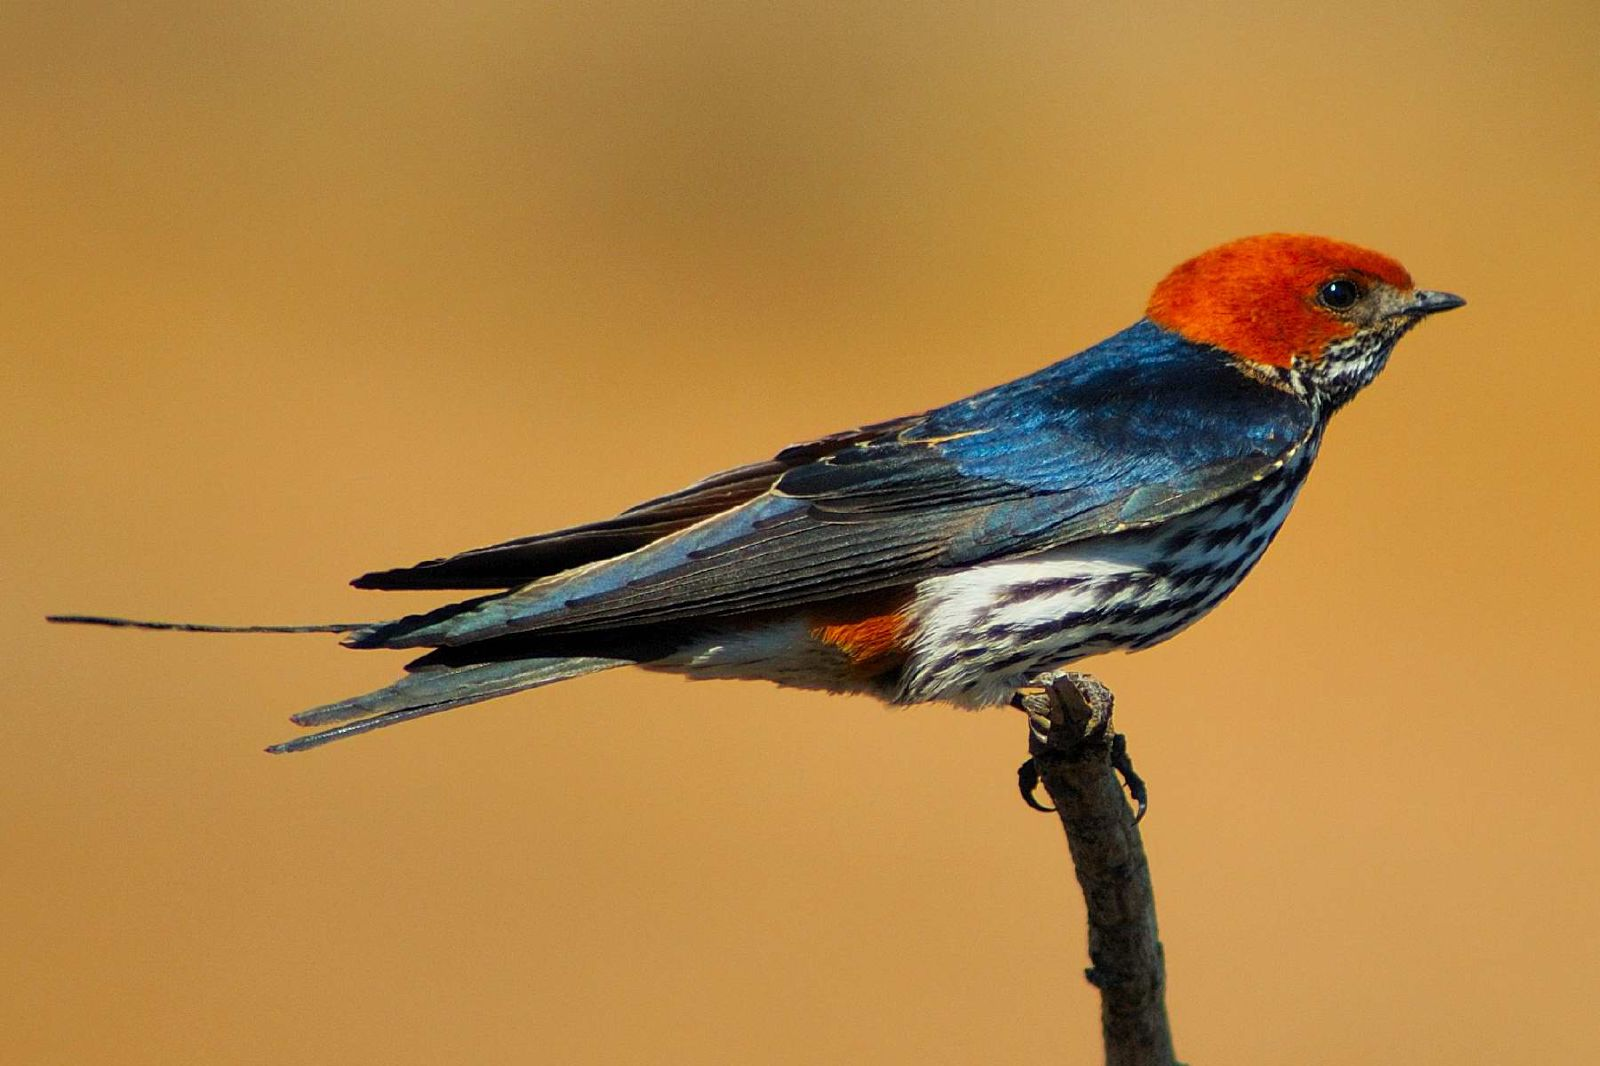
\includegraphics[width=0.5\columnwidth]{swallow.jpg} % Example image
%	\caption{European swallow.}
%\end{figure}%

%%------------------------------------------------%

%\subsection{What is the airspeed velocity of an unladen swallow?}%

%While this question leaves out the crucial element of the geographic origin of the swallow, according to Jonathan Corum, an unladen European swallow maintains a cruising airspeed velocity of \textbf{11 metres per second}, or \textbf{24 miles an hour}. The velocity of the corresponding African swallows requires further research as kinematic data is severely lacking for these species.%

%%----------------------------------------------------------------------------------------
%%	TEXT EXAMPLE
%%----------------------------------------------------------------------------------------%

%\section{Understanding Text}%

%\subsection{How much wood would a woodchuck chuck if a woodchuck could chuck wood?}%

%%------------------------------------------------%

%\subsubsection{Suppose ``chuck" implies throwing.}%

%According to the Associated Press (1988), a New York Fish and Wildlife technician named Richard Thomas calculated the volume of dirt in a typical 25--30 foot (7.6--9.1 m) long woodchuck burrow and had determined that if the woodchuck had moved an equivalent volume of wood, it could move ``about \textbf{700 pounds (320 kg)} on a good day, with the wind at his back".%

%%------------------------------------------------%

%\subsubsection{Suppose ``chuck" implies vomiting.}%

%A woodchuck can ingest 361.92 cm\textsuperscript{3} (22.09 cu in) of wood per day. Assuming immediate expulsion on ingestion with a 5\% retainment rate, a woodchuck could chuck \textbf{343.82 cm\textsuperscript{3}} of wood per day.%

%%------------------------------------------------%

%\paragraph{Bonus: suppose there is no woodchuck.}%

%Fusce varius orci ac magna dapibus porttitor. In tempor leo a neque bibendum sollicitudin. Nulla pretium fermentum nisi, eget sodales magna facilisis eu. Praesent aliquet nulla ut bibendum lacinia. Donec vel mauris vulputate, commodo ligula ut, egestas orci. Suspendisse commodo odio sed hendrerit lobortis. Donec finibus eros erat, vel ornare enim mattis et.%

%%----------------------------------------------------------------------------------------
%%	EQUATION EXAMPLES
%%----------------------------------------------------------------------------------------%

%\section{Interpreting Equations}%

%\subsection{Identify the author of Equation \ref{eq:bayes} below and briefly describe it in English.}%

%\begin{align}
%	\label{eq:bayes}
%	\begin{split}
%		P(A|B) = \frac{P(B|A)P(A)}{P(B)}
%	\end{split}					
%\end{align}%

%Lorem ipsum dolor sit amet, consectetur adipiscing elit. Praesent porttitor arcu luctus, imperdiet urna iaculis, mattis eros. Pellentesque iaculis odio vel nisl ullamcorper, nec faucibus ipsum molestie. Sed dictum nisl non aliquet porttitor. Etiam vulputate arcu dignissim, finibus sem et, viverra nisl. Aenean luctus congue massa, ut laoreet metus ornare in. Nunc fermentum nisi imperdiet lectus tincidunt vestibulum at ac elit. Nulla mattis nisl eu malesuada suscipit.%

%%------------------------------------------------%

%\subsection{Try to make sense of some more equations.}%

%\begin{align}
%	\begin{split}
%		(x+y)^3 &= (x+y)^2(x+y)\\
%		&=(x^2+2xy+y^2)(x+y)\\
%		&=(x^3+2x^2y+xy^2) + (x^2y+2xy^2+y^3)\\
%		&=x^3+3x^2y+3xy^2+y^3
%	\end{split}					
%\end{align}%

%Lorem ipsum dolor sit amet, consectetuer adipiscing elit.
%\begin{align}
%	A =
%	\begin{bmatrix}
%		A_{11} & A_{21} \\
%		A_{21} & A_{22}
%	\end{bmatrix}
%\end{align}
%Aenean commodo ligula eget dolor. Aenean massa. Cum sociis natoque penatibus et magnis dis parturient montes, nascetur ridiculus mus. Donec quam felis, ultricies nec, pellentesque eu, pretium quis, sem.%

%%----------------------------------------------------------------------------------------
%%	LIST EXAMPLES
%%----------------------------------------------------------------------------------------%

%\section{Viewing Lists}%

%\subsection{Bullet Point List}%

%\begin{itemize}
%	\item First item in a list
%		\begin{itemize}
%		\item First item in a list
%			\begin{itemize}
%			\item First item in a list
%			\item Second item in a list
%			\end{itemize}
%		\item Second item in a list
%		\end{itemize}
%	\item Second item in a list
%\end{itemize}%

%%------------------------------------------------%

%\subsection{Numbered List}%

%\begin{enumerate}
%	\item First item in a list
%	\item Second item in a list
%	\item Third item in a list
%\end{enumerate}%

%%----------------------------------------------------------------------------------------
%%	TABLE EXAMPLE
%%----------------------------------------------------------------------------------------%

%\section{Interpreting a Table}%

%\begin{table}[h] % [h] forces the table to be output where it is defined in the code (it suppresses floating)
%	\centering % Centre the table
%	\begin{tabular}{l l l}
%		\toprule
%		\textit{Per 50g} & \textbf{Pork} & \textbf{Soy} \\
%		\midrule
%		Energy & 760kJ & 538kJ\\
%		Protein & 7.0g & 9.3g\\
%		Carbohydrate & 0.0g & 4.9g\\
%		Fat & 16.8g & 9.1g\\
%		Sodium & 0.4g & 0.4g\\
%		Fibre & 0.0g & 1.4g\\
%		\bottomrule
%	\end{tabular}
%	\caption{Sausage nutrition.}
%\end{table}%

%%------------------------------------------------%

%\subsection{The table above shows the nutritional consistencies of two sausage types. Explain their relative differences given what you know about daily adult nutritional recommendations.}%

%Lorem ipsum dolor sit amet, consectetur adipiscing elit. Praesent porttitor arcu luctus, imperdiet urna iaculis, mattis eros. Pellentesque iaculis odio vel nisl ullamcorper, nec faucibus ipsum molestie. Sed dictum nisl non aliquet porttitor. Etiam vulputate arcu dignissim, finibus sem et, viverra nisl. Aenean luctus congue massa, ut laoreet metus ornare in. Nunc fermentum nisi imperdiet lectus tincidunt vestibulum at ac elit. Nulla mattis nisl eu malesuada suscipit.%

%%----------------------------------------------------------------------------------------
%%	CODE LISTING EXAMPLE
%%----------------------------------------------------------------------------------------%

%\section{Reading a Code Listing}%

%\lstinputlisting[
%	caption=Luftballons Perl Script., % Caption above the listing
%	label=lst:luftballons, % Label for referencing this listing
%	language=Perl, % Use Perl functions/syntax highlighting
%	frame=single, % Frame around the code listing
%	showstringspaces=false, % Don't put marks in string spaces
%	numbers=left, % Line numbers on left
%	numberstyle=\tiny, % Line numbers styling
%	]{luftballons.pl}%

%%------------------------------------------------%

%\subsection{How many luftballons will be output by the Listing \ref{lst:luftballons} above?}%

%Aliquam arcu turpis, ultrices sed luctus ac, vehicula id metus. Morbi eu feugiat velit, et tempus augue. Proin ac mattis tortor. Donec tincidunt, ante rhoncus luctus semper, arcu lorem lobortis justo, nec convallis ante quam quis lectus. Aenean tincidunt sodales massa, et hendrerit tellus mattis ac. Sed non pretium nibh. Donec cursus maximus luctus. Vivamus lobortis eros et massa porta porttitor.%

%%------------------------------------------------%

%\subsection{Identify the regular expression in Listing \ref{lst:luftballons} and explain how it relates to the anti-war sentiments found in the rest of the script.}%

%Fusce varius orci ac magna dapibus porttitor. In tempor leo a neque bibendum sollicitudin. Nulla pretium fermentum nisi, eget sodales magna facilisis eu. Praesent aliquet nulla ut bibendum lacinia. Donec vel mauris vulputate, commodo ligula ut, egestas orci. Suspendisse commodo odio sed hendrerit lobortis. Donec finibus eros erat, vel ornare enim mattis et.

%----------------------------------------------------------------------------------------

\end{document}
